\documentclass[12pt,letterpaper]{report}
\usepackage{sisl-suthesis}

% Todos
\usepackage{regexpatch}
\makeatletter
\xpatchcmd{\@todo}{\setkeys{todonotes}{#1}}{\setkeys{todonotes}{inline,#1}}{}{}
\makeatother

% Upright bold
\usepackage{vector}
\renewcommand{\vec}[1]{\vect{#1}}


\usepackage{csquotes}
\usepackage{dsfont}
\newtheorem{proposition}{Proposition}

% Figures
\usepackage{subcaption}

% Algorithms
\usepackage{algorithm}
\usepackage{algorithmicx}
\usepackage[noend]{algpseudocode}

% Tables
\usepackage{booktabs}
\usepackage{multirow}
\renewcommand{\arraystretch}{1.2}   
\usepackage{makecell}
\usepackage{mathtools}

% TikZ
\usepackage{tikz}
\usepackage{soul}

\usetikzlibrary{arrows,fit} % for problem diagram
\usetikzlibrary{positioning} % for problem diagram
\usetikzlibrary{arrows.meta,calc,shapes} %

\setul{0.8ex}{0.4ex}

\definecolor{c1}{rgb}{0.102, 0.3686, 0.3294}
\definecolor{c2}{rgb}{0.3216, 0.1569, 0.30196}
\definecolor{c3}{rgb}{0.7765, 0.8196, 0.77255}
\definecolor{c4}{rgb}{0.82353, 0.75686, 0.59216}
\definecolor{c5}{rgb}{0.5412, 0.0902, 0.09804}


\def \radius {5cm}
\def \stem {33}
\def \margin {10} % margin in angles, depends on the radius
\def \nsize {4cm}
\def \half {0.5cm}
\def \head {0.5cm}

\tikzset{nstyle/.style={draw, circle, minimum size=\nsize}}


% For interpretable Validation chapter:
\newcommand{\T}{\textsc{T}}
\newcommand{\F}{\textsc{F}}
\newcommand{\A}{\textsc{A}}
\newcommand{\True}{\textsc{True}}
\newcommand{\False}{\textsc{False}}
\newcommand{\Arbitrary}{\textsc{Arbitrary}}

\addbibresource{references}

%% Thesis Metadata
\dept{Aeronautics and Astronautics}


\title{Algorithms for the Safety Validation of Black-box Autonomous Systems}

\author{Anthony Corso}


% adviser and readers
\principaladviser{Mykel J. Kochenderfer}
\firstreader{Dorsa Sadigh}
\secondreader{Marco Pavone}


\begin{document}
\beforepreface

% - Thesis outline
%     - 20-24 pages on chapter 2
%     - Omit Related work in the chapter sections
%     - Replace conclusion with discuss - can relate to prior approaches 
%         - First paragraph is summary and then you can talk about whatever
%         - Talk about implementations in approach, background, 

\prefacesection{Abstract}
Autonomous systems have the potential to improve safety and efficiency in safety-critical domains such as transportation, and medicine. Since human lives are at risk in these applications, we require rigorous safety validation before deployment. Traditional safety validation approaches such as real-world testing and scenario-based testing in simulation are not scalable to complex systems and environments and may miss unforeseen failures. Formal verification techniques also lack the scalability required for large scale autonomy. 

% black box safety validation
The thesis address the safety validation problem with black-box sampling techniques, which assume no knowledge of the design of the autonomous system. The system takes actions in a stochastic environment and failures are discovered by sampling environmental disturbances. The black-box assumption allows for better scalability to complex autonomous systems and sampling can be combined with machine learning to discover unforeseen failures. Previous black-box safety validation approaches have been based on optimization, path-planning, reinforcement learning and importance sampling. Although successful for many safety validation applications, existing algorithms may have poor interpretabiliy, scalability, and efficiency. 

% Interpretability
Black-box sampling approaches can provide example failure trajectories but do not provide a high-level description of failures, as scenario-based approaches do. We present a new technique for generating failure descriptions in the form of signal temporal logic specifications on the environment disturbances. The specifications are optimized with genetic programming to produce failure examples and can used to gain insight into why a failure occurred. 

% Scalability
A key contribution of this thesis is the proposal and analysis of a state-dependent sampling distribution to approximate the distribution over failures. The use of the state of the environment produces a more efficient sampling distribution than baseline importance sampling approaches, but may be limited by the size of the state space. To improve scalability, we propose a decomposition technique for multi-agent validation tasks. Each subproblem is solved independently and the results are combined for better performance than learning from scratch.

% Efficiency
During the design of an autonomous system, safety validation is performed repeatedly, requiring a large computational expense. We propose a transfer learning technique that can reduce the number of required samples and lead to better performance. Knowledge from previous validation tasks is transferred to new tasks in the form of value functions that are combined using a learned set of attention weights. Results show improved knowledge transfer between tasks compared to baseline techniques. 

The safety validation algorithms presented in this work are tested on two gridworld scenarios and two driving scenarios. A simple gridworld scenario is used to illustrate important safety validation concepts while a gridworld with multiple adversaries is used as a test case for multi-agent validation. A rules-based autonomous driving policy is tested in a crosswalk scenario with a pedestrian and a T-intersection scenario with multiple vehicles. It is shown that the presented algorithms can improve the interpretability, scalability and efficiency of safety validation.

\prefacesection{Acknowledgments}
This dissertation would not have been possible without the help of many people including my family, my friends, and everyone at Stanford who makes research possible. 
First, I would like thank my reading committee, Professor Dorsa Sadigh and Professor Marco Pavone, for providing valuable feedback on my research, defense, and dissertation. Their perspective and inquiry helped hone my research direction, and both have provided valuable advice and opportunities outside of my dissertation work. Then, I would like to thank my advisor Professor Mykel Kochenderfer for mentoring me in research and in life. Mykel helped me discover the wonders of machine learning and decision making, taught me how to communicate more clearly and succinctly, and demonstrated how to live a life full of passion, gratitude, and kindness. I am incredibly grateful for everything I have learned from Mykel, and look forward to our continued collaborations as co-workers and friends. 

My first three years at Stanford were funded by the Lillie Family Stanford Graduate Fellowship. Without that fellowship I may not have attended Stanford, so I thank the Aeronautics and Astronautics department for nominating me and the Lillie Family for providing the funds. I want to thank the Stanford Center for AI safety for funding my dissertation research, and specifically NVIDIA for providing the funding and research direction. Thank you to Michael Cox and Ahmed Nassar at NVIDIA for always providing feedback on my work and supporting the safety center. Thank you to NASA Ames and Dr. Ritchie Lee for supporting my summer internship at NASA Ames and collaborating on several projects. Lastly, I would like to thank the NASA University Leadership Initiative for supporting my last quarter of research, and Professor Marco Pavone for providing the opportunity.

I have had the opportunity to collaborate with many amazing friends and researchers. I would first like to thank Dr. Ashish Goel, Dr. Paul Tarantino and especially Dr. Siddarth Krishnamoorthy for giving me valuable research experience and advice as I navigated my first several years of graduate school. Thank you to Dr. Jeremy Morton, Professor Freddie Witherden, Mark Koren, Xiaobai Ma, Peter Du, and Professor Katherine Driggs-Campbell, for collaborating on my first research projects as a member of SISL. Thank you to Dr. Ritchie Lee for developing many of the ideas that I built on for my thesis, and for being a valuable research mentor. Thank you to Robert Moss, Dr. Alex Koufos, Dr. Maxime Bouton, Dr. Di Wu, and all of the other SISL members who gave me advice and feedback on my research. Lastly, thank you to Sydney Katz and Chris Strong for helping me develop my next stage of research projects. 

Thank you to my roommate Stephen for being a supportive and easy going living partner. Thank you to Krishna, Jasper, Jenny, John, and all of the other friends I have met (and climbed with) at Stanford, as well as my friends from Harvey Mudd and back home in Oregon. Thank you to my girlfriend Emma. She provided an endless source of advice, support, and love during my time in graduate school. Thank you for always having my back, cheering me on, and always being willing to share a laugh or go on an adventure. 

Lastly, thank you to my family, to whom I truly owe everything. Thank you for teaching me to be the person I am today and providing me all the support I have needed to pursue my dreams. Thank you to my sister Amie, who can always make me feel better when I am in a bad spot, and whose enthusiasm about the work we do always leads to great conversations. Thank you to my Mom and Dad who have always encouraged me to think for myself and work hard for the things that are important. I love you all.


\afterpreface

\chapter{Introduction}
% Intro paragraph. 1 sentence on why the topic, why is it challenging, what this thesis does, outline of the chapter
With the recent increase in capability of autonomous systems, they are being deployed in safety-critical domains such as autonomous driving, aviation, and medicine where the consequences of operational errors include loss of property or human life. Ensuring the safe operation of safety-critical autonomous systems is a necessary step before deployment, but remains a significant technical challenge due to the complexity of systems and the environments in which they operate. This thesis presents scalable, interpretable, and efficient methods for validating the safety of autonomous systems in simulation. This chapter first discusses the general problem of autonomous system safety and argues that safety validation through black-box sampling plays a crucial role. The next sections goes on to give an overview of the challenges of black-box to safety validation approaches, followed by the contributions and outline of the thesis.

\section{Safety Validation of Autonomous Systems}

% Why should we want autonomous systems
Introducing autonomy into safety-critical domains has the potential to improve both safety and efficiency. Driving accidents killed \num{1.35} million people in 2016~\cite{world2019global}, and approximately \num{94}\% of accidents between 2005--2007 in the US were due to driver error~\cite{singh2015critical}. Autonomous aircraft collision avoidance systems were put into place after a series of devastating mid-air collisions~\cite{federal2011introduction} and have been shown to reduce the (already rare) risk of mid-air collision by at least a factor of 3~\cite{arino2002studies}. The next generation of aircraft collision avoidance systems will improve safety and function in the higher-density airspaces of the future~\cite{kochenderfer2012next}.

% There are risks as well
Although the upside of automation can be large, there are serious risks involved in deploying such systems. On March 18, 2018, a vehicle controlled by an autonomous system struck and killed a pedestrian in Arizona. A report of the incident found that the vehicle observed the pedestrian as an unknown object \num{6} seconds prior to the collision but failed to classify the pedestrian and gave varying predictions for the future path of travel. It took an additional \num{4.7} seconds for the autonomous system to determine that emergency braking was required~\cite{board2018preliminary}. Another example of risk comes from aircraft collision avoidance systems. Aircraft collision avoidance systems have the potential to induce a small number of mid-air collisions that would not have otherwise occurred~\cite{arino2002studies}. The number of induced collisions is much smaller than the number of prevented collisions, but these induced collisions highlight the possibility of bad outcomes for systems that are improperly designed, tested or deployed.

\begin{figure}[!t]
\centering
\resizebox{0.9\textwidth}{!}{%
\begin{tikzpicture}
% Arrows
\draw[fill=gray!20,line width=1pt] (144:\radius + \half) arc (144:72 + \stem:\radius+\half) -- (72 + \stem:\radius+\half+\head) -- (72 + \stem - \margin:\radius) -- (72+\stem:\radius-\half-\head) -- (72+\stem:\radius-\half) arc (72+\stem:144:\radius-\half)--cycle;

\draw[fill=gray!20,line width=1pt] (72:\radius + \half) arc (72:0 + \stem:\radius+\half) -- (0 + \stem:\radius+\half+\head) -- (0 + \stem - \margin:\radius) -- (0+\stem:\radius-\half-\head) -- (0+\stem:\radius-\half) arc (0+\stem:72:\radius-\half)--cycle;

\draw[fill=gray!20,line width=1pt] (0:\radius + \half) arc (0:-72 + \stem:\radius+\half) -- (-72 + \stem:\radius+\half+\head) -- (-72 + \stem - \margin:\radius) -- (-72+\stem:\radius-\half-\head) -- (-72+\stem:\radius-\half) arc (-72+\stem:0:\radius-\half)--cycle;

\draw[fill=gray!20,line width=1pt] (-72:\radius + \half) arc (-72:-144 + \stem:\radius+\half) -- (-144 + \stem:\radius+\half+\head) -- (-144 + \stem - \margin:\radius) -- (-144+\stem:\radius-\half-\head) -- (-144+\stem:\radius-\half) arc (-144+\stem:-72:\radius-\half)--cycle;

\draw[fill=gray!20,line width=0pt] (-144:\radius + \half) arc (-144:-216 + \stem:\radius+\half) -- (-216 + \stem:\radius+\half+\head) -- (-216 + \stem - \margin:\radius) -- (-216+\stem:\radius-\half-\head) -- (-216+\stem:\radius-\half) arc (-216+\stem:-144:\radius-\half)--cycle;


\node[nstyle, fill=c1!80, ] at (144:\radius) (test)
{
\includegraphics[height=2.\nsize]{figures/introduction/blueprint}};
\node[text width=8cm, anchor=west] at (-13cm, 4.4cm) {\setulcolor{c1} {\LARGE{\ul{\bf 1. Define Requirements}}} \\ 
\Large
\begin{itemize}
\item Temporal logic
\item Dangerous states
\end{itemize}
};

\node[nstyle, fill=c2!80] at (72:\radius) {
\includegraphics[height=2.\nsize]{figures/introduction/eng}};
\node[text width=8cm, anchor = west] at (3.6cm, 6cm) {\setulcolor{c2} {\LARGE{\ul{\bf 2. Design Effort}}} \\ 
\Large
\begin{itemize}
\item Machine learning
\item Engineering
\end{itemize}
};

\node[nstyle, fill=c3!80] at (0:\radius) {
\includegraphics[width=2.\nsize]{figures/introduction/tree}};

\node[text width=8cm] at (6:\radius + 6cm) {\setulcolor{c3} {\LARGE{\ul{\bf 3. Generate  Testcases}}} \\ 
\Large
\begin{itemize}
\item Unit tests
\item Automated testing
\end{itemize}
};

\node[nstyle, fill=c4!80] at (-72:\radius) {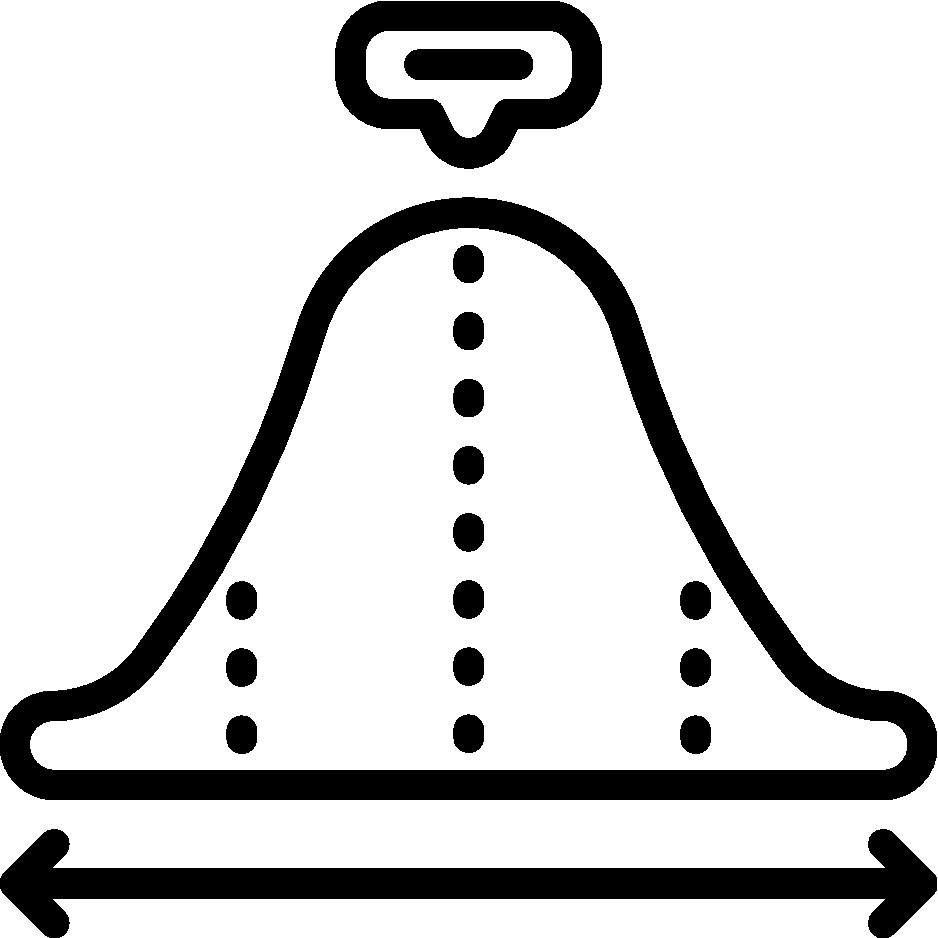
\includegraphics[height=2.\nsize]{figures/introduction/graph}};

\node[text width=10cm] at (-36:\radius + 6.2cm) {\setulcolor{c4} {\LARGE{\ul{\bf 4. Evaluate  Performance}}} \\ 
\Large
\begin{itemize}
\item Failure probability
\item Failure severity
\end{itemize}
};


\node[nstyle, fill=c5!80] at (-144:\radius) {
\includegraphics[height=2.\nsize]{figures/introduction/head}};

\node[text width=8cm,anchor=west] at (-13.5cm, -3.5cm) {\setulcolor{c5} {\LARGE{\ul{\bf 5. Interpret Failures}}} \\ 
\Large
\begin{itemize}
\item Failure classification
\item Root cause analysis
\end{itemize}
};
\end{tikzpicture}
}
\caption{The design cycle of an autonomous system.  }
\label{fig:design_cycle}
\end{figure}

% Description of the design cycle of an autonomous system
To understand how to incorporate safety into autonomous system, we must first understand how such systems are designed. The design cycle of autonomous systems is shown in \cref{fig:design_cycle}. The first step in system design is the \emph{definition of requirements} which may include specifications on performance, safety, interpretability, and more. Then, some \emph{design effort} is expended to develop a prototype of the system. Modern and future autonomous system design will usually involve a combination of machine learning and traditional engineering. Once a prototype of the system is available, it must undergo \emph{testing} in the form of unit tests of specific components and integration tests of the larger subsystems. The generation of these test cases can be done from expert knowledge or can be automated. Based on the results of the tests, the system is \emph{evaluated} on any number of performance metrics. Safety metrics may include the probability the system violates its safety specification (referred to as a \emph{failure}) or the severity of observed failures. At this point, if the systems meets all required performance and safety specifications, it can be deployed. If not, then the failures of the system need to be \emph{interpreted} to discover discover broad categories of failures, called \emph{failure modes} and to perform root-cause analysis to discover flaws in the system. Once failures are identified and categorized, the system requirements may need to be updated and the cycle continues until the system is ready for deployment. 


%Safety of an autonomous systems should be incorporated at all stages of the development
Safety can and should be incorporated at all stages of the design cycle. This thesis focuses primarily on \emph{safety validation}, which covers the stages of testing, performance evaluation and failure interpretation, but we will first briefly describe how safety can be included in the stages of requirement definition and design. 

The most straightforward way of including safety in the definition of system requirements is to identify what is meant by a failure and stipulate a maximum allowable failure probability or failure severity. Although this type of requirement provides a concrete safety goal, it does not necessarily help the design process more easily produce a safe system. A thorough analysis of the environment and system may allow for a set of specifications that can guarantee safety under a set of assumptions. For autonomous driving, the responsibility-sensitive safety model~\cite{shalev2017formal} and the safety force field model~\cite{nister2019safety} both develop a set of rules that restrict the actions of a driving agent to ensure safety. These specifications are not comprehensive enough to define a complete driving policy, but an agent based on machine learning may be trained to satisfy a goal while respecting such specifications~\cite{sadigh2014learning,bouton2019reinforcement}.

Designing a safe autonomous system with machine learning can be especially challenging. Approaches to improve safety of machine-learned systems include defining objectives that adequately penalize rare but catastrophic failures~\cite{moldovan2012risk} or are risk-aware~\cite{tamar2014policy}, learning from safe human demonstrations~\cite{abbeel2005exploration}, and training on adversarial examples~\cite{goodfellow2014explaining}. For agents that continue to learn in their operational environment, they will need to perform safe exploration which can be done by only allowing exploratory actions that are reversible~\cite{moldovan2012safe}, through active learning~\cite{garcia2013safe}, or through uncertainty-awareness~\cite{sui2015safe}. For a good overview on the topic of safe reinforcement learning see \textcite{garcia2015comprehensive} and \textcite{amodei2016concrete}. 


% Compare and contrast different techniques (Testing in the real world, scenario-based or unit tests, formal methods, black both approaches)
Safety validation is performed on an existing prototype of a system and can have several objectives such as discovering failures of the system, computing the likelihood that the system fails, or understanding which environmental factors might lead to a system failure. There are many techniques that are used for safety validation, each with pros and cons. Below we discuss four categories of validation approaches. 

\paragraph{Scenario-based testing} Usually done in simulation, scenario-based testing is a form of unit testing where scenarios are developed to challenge specific behaviors or components of an autonomous system. These scenarios can be constructed from real-world data or through expert knowledge, and can be designed to focus on potential weaknesses of the system. Scenario-based testing can be used for regression testing, where the same suite of scenarios is applied to the system each time it changes to make sure no old failure modes have been re-introduced. The downside to scenario-based testing is the possibility of missing important failure cases because they were not included the suite of tests. Important tests may be excluded due to incorrect assumptions about the environment or due to the difficulty of predicting failures caused by the complex interaction of many components.

\paragraph{Real-world testing} In real-world testing, a prototype of the system is used in an environment that is as close as possible to the intended deployment environment. For autonomous driving this may be a closed course or an area of a city that has already undergone extensive mapping. Usually, the system will be equipped with extra safety features to mitigate risk. This form of testing is critical before deployment because there may be complications that arise when moving from simulated environments to the real world. The downside to real-world testing is the high cost (in both time and other resources) and the high consequence if the system behaves unsafely.

\paragraph{Formal verification} Formal verification techniques can provide mathematical proofs about system safety under a set of assumptions. The system must first be described by a mathematical model such as a finite state machine, computer code, or the parameters and architecture of a neural network. The model is checked against a safety specification usually written in a temporal logic. In \emph{model checking} all inputs to the system are exhaustively checked to discover any outputs that violate the safety specification. If there are no violations, then the system is concluded to be safe. Another approach is \emph{deductive verification} where a proof of safety is constructed through a series of intermediate theorems about the behavior of the system. These proofs are often constructed with automated theorem provers. Formal verification gives the highest degree of confidence in the safety of a system under the assumption that the mathematical model adequately represents the true system. The main drawback to formal verification is that it may not scale well to systems with large or continuous state spaces operating in environments with a large number of inputs to the system. 

\paragraph{Black-box sampling and learning} Black-box sampling techniques involve repeatedly simulating the system in a stochastic model of the environment to discover failures. The term \emph{black-box} comes from the assumption that we do not know anything about the structure of the system and can only interact with it through inputs and outputs. This assumption allows black-box sampling approaches to be applied to complex systems. In the case where failures are rare, random simulation may be inefficient for finding failure examples or computing the probability of failure. In this case, learning techniques can be applied to iteratively improve the stochastic parameters of the environment to make failures more likely to occur. The downside to black-box sampling techniques and learning is that we will never be fully confident in the safety of the system, and instead must rely on probabilistic statements of safety. 

While all of the safety validation approaches are useful in different circumstances, we focus on black-box safety validation due to its favorable scalability and the ease with which it can be combined with powerful machine learning algorithms.


\section{Challenges to Black-Box Safety Validation}
There are many challenges for algorithms that use black-box sampling including accurate modeling of the system and the environment, efficiency in the number of simulations required, and interpretability of discovered failures. 

% Challenges of modeling the system and environment
Although not discussed in detail in the rest of this thesis, the challenge of accurately modeling an autonomous system interacting with a physical environment is crucial to the success of simulation-based validation strategies. To accurately model the physical world, we need to define the dynamics of a large number of continuous and discrete variables. In general, the dynamics may be stochastic and nonlinear which can pose significant computational challenges. In addition, there may be other decision-making agents (such as humans) in the environment whose decisions we must model. Consider, for example, that we wish to test an autonomous vehicle (AV) navigating through an intersection with human drivers. To do this in simulation, we must accurately model the 3D environment, the dynamics of the AV and the other vehicles, the functioning of all sensors on the AV, the behavior of other drivers and pedestrians, and more. To address these modeling challenges, we can make simplifying assumptions about the environment, learn models from real-world data, or construct models from first principles. Although there are many open questions in the modeling literature, we assume that for any system we wish to validate, there already exists a sufficiently good simulator of the environment and that any source of stochasticity (such as the behavior of other agents) is accurately modeled. 

% Needle in the haystock problem - Combinatorial complexity
Once a simulator of the system and the environment is defined, the next biggest challenge is efficiently discovering failures of the system due to variations in the environment over time. Suppose that the stochastic elements of the environment can be described by $M$ disturbance variables over $T$ timesteps. If each disturbance can take on $K$ values (assuming a discretization for continuous variables), then the number of possible disturbance trajectories is $K^{MT}$. In the worst case, we must enumerate a combinatorially large number of possibilities to discover a failure, which becomes intractable for even moderate values of $M$ and $T$. The problem becomes more challenging when the system or the environment is stochastic, so the same disturbance trajectory may have different outcomes for different trials. To handle stochasticity or to help guide the search for failures, we may wish to consider the state of the environment when choosing disturbances by constructing a policy that maps states to disturbances. If we assume that the environment has $N$ states and that the policy depends only on the current state (Markov assumption), then the total number of possible policies is $K^{MN}$. In practice, the problem of combinatorial complexity may be overcome through the use of search heuristics based on optimization, path-planning or reinforcement learning, which will be discussed in detail in the next chapter. These techniques have demonstrated good empirical results but offer no guarantees of finding failures without exhaustive search.

% Sample complexity for probabilistic environments
For some systems, we may not require safety for all possible disturbances but instead specify a maximum probability of failure assuming a distribution over disturbances. For example, no AV can avoid an accident in all scenarios~\cite{shalev2017formal} but we hope to develop AVs with a failure probability of less than \num{e-9} per hour~\cite{koopman2016challenges}. The benefit of this approach is that estimating the probability of failure is independent of the number of possible disturbance and state trajectories, and only depends on the sampling distribution and number of samples. The number of samples required, however, may still be intractably large. Consider the goal of verifying that the probability of failure of an AV in a given driving scenario is no larger than \num{e-9}. To be confident in this conclusion using Monte Carlo estimation, we would require on the order of \num{e9} samples~\cite{koopman2016challenges}. This number of samples may be much lower than an exhaustive search of disturbance trajectories, but is still infeasible when dealing with computationally expensive driving simulators, and the need to repeat this process for many driving scenarios and versions of the AV. To overcome this challenge, \emph{importance sampling} approaches construct a new sampling distributions where failures are more likely, leading to better sample efficiency. 

% Interpretability
In order to uncover the flaws in a system, we must first understand under what circumstances the system fails. When performing black-box safety validation we generate failure trajectories that are high dimensional (each with $M \times T$ dimensions) so they may not provide any insight into what caused the system to fail. Even with many failure examples it is not clear how to induce the causal environmental factors that lead to failure, making it difficult to understand what needs to be fixed in the system. Currently, the best approaches for understanding what caused a system to fail is the use of unit tests that test specific component behavior, or failure classification that groups failure examples into similar failure modes. 

The algorithms presented in this thesis make progress toward better scalability, efficiency and interpretability for black-box safety validation. The intended goal of these algorithms is to develop more useful safety validation tools to help develop safer autonomy.


\section{Contributions}

% Intro paragraph
This thesis provides a general formulation of the problem of safety validation for black-box autonomous systems. This formulation helps categorize different algorithms for safety validation and provides a framework in which to develop new safety validation algorithms. We address some of the major challenges of black-box safety validation--interpretability, scalability, and sample efficiency--by developing new algorithms.

% paragraph on interpretable validation
To address the problem of interpretability, we introduce \emph{interpretable safety validation}, an algorithm that produces human-understandable descriptions of scenarios that lead to failure. Traditional safety validation approaches may return a number of failure examples, but these examples can be high-dimensional and therefore be difficult to interpret and analyze. A simple description of the scenarios that lead to failure allows engineers to quickly identify flaws in the system and to generate a large number of failure examples for further analysis. 

% Paragraph on scene decomposition
Safety validation of multi-agent systems is hindered by the exponential increase in states and actions with the number of agents in an environment. We address the problem of scalability by assuming multi-agent systems can be decomposed into a set of smaller problems that are easier to solve. The solutions to these smaller problems can then be recombined to more efficiently solve the full-scale safety validation problem. Our decomposition approach is shown to increase the efficiency of safety validation tasks in an autonomous driving setting.

% Paragraph on iterative safety validation
When many related systems need to be validated, conventional approaches require the validation to start from scratch for each system, resulting in low sample efficiency. By applying techniques from transfer learning, we demonstrate that results from previous validations can be used to accelerate the process of validation of a new system, event when the systems have significantly different behavior. For autonomous systems that are under continuous development, or for an analysis of many related systems, our approach can provide a large improvement in sample efficiency.


\section{Outline}
The rest of the thesis is organized as follows. 

% Chapter 2 - Background
Chapter 2 formulates the problem of safety validation and presents the notation used in the rest of this work. It then provides an overview of the existing techniques for the safety validation of black-box autonomous systems, categorized into approaches based on optimization, path-planning, reinforcement learning, and importance sampling. The motivations, benefits and drawbacks of each category are discussed and specific algorithms are outlined. 

% Chapter 3 - Sample Systems
Chapter 3 discusses the practical considerations involved in formulating a safety validation problem from a system and simulator. We present four concrete example systems to be used in the remainder of the thesis. The first two examples are gridworld problems with simple dynamics and are used to illustrate the core ideas of safety validation. The second two examples involve autonomous vehicles in complex environments and are used to demonstrate safety validation on a larger scale. 

% Chapter 4 - Interpretable Safety Validation
Chapter 4 argues for the importance of interpretable safety validation strategies and proposes a new interpretable safety validation algorithm based on temporal logic and expression optimization algorithms. The algorithm discovers temporal logic descriptions of disturbances that lead to failure. These descriptions are used to understand flaws in the system and to generate examples of high-likelihood failures. The algorithms is demonstrated on two autonomous driving scenarios. 

% Chapter 5 - Importance sample for sequential decision making problems
Chapter 5 introduces the task of learning the optimal sampling distribution for estimating the probability of failure of sequential decision-making systems. We derive the optimal distribution in the case of a deterministic Markov simulator and suggest an effective distribution for stochastic or non-Markov systems. The proposed sampling distributions are able to generate a high rate of failures and quickly converge when estimating the probability of failure. These results are demonstrated through experimentation in the gridworld and autonomous driving settings.

% Chapter 6 - Scalability through scene decomposition
Chapter 6 outlines the scalability challenges of computing the optimal sampling distribution for estimating the probability of failure and proposes a decomposition approach to improve scalability. When an environment consists of multiple interacting agents, we can model the problem as a combination of subproblems, each involving only two agents. The optimal sampling distribution can be computed for each subproblem and the optimal sampling distribution for the combined problem can be estimated through a combination of the subproblem solutions and a correction factor to account for multi-agent interactions. We demonstrate that this approach can more efficiently solve the safety validation problem of multi-agent systems through experimentation with a driving scenario with \num{5} agents. 

% Chapter 7 - Efficient iterative safety valiidation
Chapter 7 describes a new approach for improving sample efficiency of safety validation algorithms when they are applied to multiple systems that share some characteristics. The approach is based on \emph{transfer learning}, where the insights gained during the safety validation of one system are applied to another, insofar as they are applicable. We demonstrate improvements in initial and final performance of learning-based safety validation algorithms and a reduction in the number of training steps required.

% Chapter 8 - Conclusion and future work
Finally, Chapter 8 provides a summary of the contributions of the thesis and discusses some of the remaining challenges for safety validation of black-box autonomous systems. Some possible future directions to address those challenges are presented. 


\chapter{Background}
In order to develop algorithms for safety validation of black-box systems, we need to mathematically formalize the problem. In this chapter we formulate safety-validation as the interaction between two decision-making agents: the system and the adversary. We define notation and formalize the underlying goals of different safety validation algorithms. With the goals defined, we survey the existing literature on black-box safety validation and categorize different algorithms into four types: optimization, path planning, reinforcement learning and importance sampling. 

\section{Problem Formulation}

Suppose we have an autonomous system under test (referred to as the \emph{system}) that takes actions $a \in A$ in an \emph{environment} with state $s \in S$. Actions are selected based on observations $o \in O$ of the environment. The system interacts with the environment over discrete time $t \in \{1, \ldots, t_{\rm max}\}$. We denote a state trajectory up to time $t$ as $\vec{s}_{1:t} = [s_1, \ldots, s_t]$, an observation trajectory $\vec{o}_{1:t} = [o_1, \ldots, o_t]$, and an action trajectory $\vec{a}_{1:t} = [a_1, \ldots, a_t]$. The system may be modeled by a function $\mathcal{M}$ that maps an observation trajectory to an action
\begin{equation}
    a_t = \mathcal{M}(\vec{o}_{1:t}) \text{.} \label{eq:system} 
\end{equation}

An \emph{adversary} $\mathcal{A}$ produces disturbances $x \in X\subseteq \mathbb{R}^n$ in the environment with the goal of causing the system to fail. A disturbance trajectory is denoted $\vec{x}_{1:t}$ or just $\vec{x}$. Although we present the most general case of disturbances as a trajectory of inputs to the environment, $\vec{x}$ may also represent static environment parameters or initial conditions. 

The adversary can use full or partial knowledge of the environment state to determine the next disturbance such that
\begin{equation}
    x_t = \mathcal{A}(\vec{s}_{1:t}) \text{.} \label{eq:adversary}
\end{equation}
Adversaries that use the system state require an environment that is constructed to provide that information. In cases where the state information is unavailable (possibly due to the simulator implementation or privacy concerns), the adversary must produce disturbance trajectories based solely on the outcomes of past trajectories. 

The environment state evolves over time and is influenced by the actions of the system and the disturbances from the adversary. The environment is modeled by $\mathcal{E}$, where
\begin{equation}
    s_{t+1}, o_{t+1} = \mathcal{E}(\vec{a}_{1:t}, \vec{x}_{1:t}) \text{.} \label{eq:environment}
\end{equation} 
The interaction between the system, the environment, and the adversary is depicted in \cref{fig:problem}.

\begin{figure}[!t]
\centering
\resizebox{\columnwidth}{!}{% TikZ diagram for black-box safety validation problem formulation.

\tikzset{
    >={Latex[width=2mm,length=2mm]},
        base/.style = {rectangle, rounded corners, draw=black,
        minimum width=1cm, minimum height=1cm,
        text centered},
    block/.style = {base, minimum width=2.5cm, minimum height=1.5cm},
    sutstyle/.style = {block, fill=gray!50},
    envstyle/.style = {block, fill=white}, % green!15
    advstyle/.style = {block, fill=red!15},
}

\begin{tikzpicture}
    [
        node distance=5.5cm,
        every node/.style={font=\large},
        align=center
    ]

    \node (system) [sutstyle] {System\\ $\mathcal{M}$}; % System
    \node (environment) [envstyle, right of=system] {Environment\\ $\mathcal{E}$}; % Environment
    \node (adversary) [advstyle, right of=environment] {Adversary\\ $\mathcal{A}$}; % Adversary

    \draw[->] (system) -- (environment) node [pos=0.45,above] {{\small action $a$}};
    \draw[->] (adversary) -- (environment) node [pos=0.45,above] {{\small disturbance $x$}};
    \draw[->] (environment.south) ++(-0.5,0) -- +(0,-1) -| node[pos=0.25,below] {{\small observation $o$}} (system);
    \draw[->] (environment.south) ++(0.5,0) -- +(0,-1) -| node[pos=0.25,below] {{\small state $s$}} (adversary);
\end{tikzpicture}}
\caption{Model of the safety validation problem.}
\label{fig:problem}
\end{figure}

Some safety validation tasks require that the environment has a model of the disturbances. Let $p(\vec{x})$ be the probability density of the disturbance trajectory $\vec{x}$. If the disturbances are independent across time, then it is sufficient to define the density over a single disturbance $p(x)$, or if the disturbances depend only on the state it is sufficient to define $p(x \mid s)$. The disturbance model can be constructed through expert knowledge or learned from data.

In this work, we assume that the environment and the system are fixed, making disturbances the only way to affect the system. Therefore, from the point of view of the adversary, the system and environment can be combined into a single function $f$ that maps disturbance trajectories into state trajectories
\begin{equation}
\vec{s} = f(\vec{x}) \text{.}
\end{equation}
Some algorithms require the ability to simulate a disturbance $x_t$ for a single timestep from a state $s_t$. We denote the simulation step
\begin{equation}
    s_{t+1} = f(s_t, x_t) \text{.}
\end{equation}

The desired operation of the system is described by one or more specifications $\psi$ which are either written in a formal specification language or designed ad hoc. We overload the notation $\psi$ to be the set of state trajectories that satisfy the specification and write $\vec{s} \in \psi$ when the state trajectory satisfies the specification and $\vec{s} \not \in \psi$ when $\vec{s}$ violates the specification.

\paragraph{Temporal Logic.} Safety specifications are often defined as statements in temporal logic, a category of languages used to reason about the temporal behavior of dynamic systems. Temporal logic statements evaluate to a Boolean for a (potentially infinite) sequence of states, or \emph{path}. Temporal logic statements are generated from a set of propositional variables, logical operators and temporal modal operators. The logical operators include \emph{conjunction} ($\land$), \emph{disjunction} ($\lor$), and \emph{negation} (\lnot), while the temporal modal operators depend on the type of temporal logic. 

% Different types of temporal logic
Linear temporal logic (LTL)~\cite{pnueli1977temporal} includes the temporal modal operators \emph{always} $\square \psi$ ($\psi$ is true on the entire path), \emph{eventually} $\lozenge \psi$ ($\psi$ is true anywhere on the path), and \emph{until} $\psi_1 \mathcal{U} \psi_2$ ($\psi_1$ holds at least until $\psi_2$ becomes true on the path). Computational tree logic (CTL)~\cite{clarke1981design} and its more expressive counterpart CTL$^*$~\cite{emerson1986sometimes} reason about futures with branching paths and therefore include the temporal modal operators of \emph{all} $A \psi$ ($\psi$ is true on all possible paths originating from the current state) and \emph{exists} $E \psi$ ($\psi$ is true on at least one path originating from the current state). Metric temporal logic (MTL)~\cite{koymans1990specifying} allows for the temporal modal operators to be applied to a finite time interval $I$, denoted with a subscript ($\square_I \psi$ means $\psi$ always holds in the interval $I$). Signal temporal logic (STL)~\cite{maler2004monitoring} extends the set of propositional variables to allow for real-valued signals, which are converted to Boolean statements using the comparison operators ($<$, $\leq$, $=$, $\geq$, $>$). For a concrete example, consider a real-valued variable $d$ that represents the absolute distance between two vehicles. If we want to encode the safety specifications ``the vehicles will not collide in the next 30 seconds" we can write
\begin{equation}
    \psi := \square_{[0,30} (d > 0) \text{.}
\end{equation}



\section{Safety Validation Tasks}

Safety validation is concerned with finding disturbance trajectories that cause a system to failure and reasoning about the probability of those failures. We have identified four common safety validation tasks which are formally defined below.

\paragraph{Falsification:} Find a counterexample to the specification. 
\begin{equation} 
\vec{x} \quad \text{s.t.} \quad f(\vec{x}) \not \in \psi
\end{equation}

\paragraph{Most likely failure analysis:} Find the most likely counterexample.
\begin{equation}
\underset{\vec{x}}{\argmax} \quad p(\vec{x}) \quad \text{s.t.} \quad f(\vec{x}) \not \in \psi
\end{equation}

\paragraph{Probability of failure estimation:} Compute the probability that the system fails.
\begin{equation}
P_{\rm fail} = \mathbb{E}_{p(\vec{x})}\left[ \mathds{1}{\{ f(\vec{x}) \not \in \psi \}} \right]
\end{equation}

% \paragraph{Approximating the optimal sampling distribution:} Create a distribution that efficiently computes the probability of failure. 
% \begin{equation}
% \min_{q} \text{Var}\left[ \frac{1}{N} \sum_{i=1}^N \frac{p(\vec{x}_i) \mathds{1}{\{ f(\vec{x}_i) \not \in \psi \}}}{q(\vec{x}_i)} \mid  \vec{x}_i \sim q \right]
% \end{equation}

Note that the tasks are specified in order of increasing difficulty and utility. The first two tasks involve finding individual failure examples, with most-likely failure analysis being more challenging due to the need for maximizing the probability of the failure trajectory. To estimate the probability of failure, we need to discover many failure examples, each with relatively high likelihood. Thus, if we can generate a sampling distribution that produces many high-likelihood failure examples (solving the failure probability task), then we have effectively solved the task of falsification and most likely failure analysis.  

\section{Existing Approaches}

% Naive approaches
The naive approach to finding failures of an autonomous system assumes that each disturbance trajectory leads to a binary outcome: failure or not failure. If that is the case, then the best we can do is search randomly over the space of disturbance trajectory until a failure is discovered. The space of disturbance trajectories scales exponentially with the dimension of the disturbance space and the length of the trajectories, so exhaustive search quickly becomes intractable. Fortunately, we can often gather more information about how close the system was to failure and use that information to guide the search toward failure trajectories. We encode the information as a safety metric $c_{\text{safe}}(\vec{s})$ over a state trajectory $\vec{s}$, with lower values indicating less safety. 

% Measuring levels of safety
The design of a safety metric is specific to the application and the type of failure. For collision avoidance applications in autonomous driving or aviation, a common choice is the \emph{miss distance} (the closest physical distance between two agents)~\cite{lee2015adaptive,koren2018adaptive} or the \emph{time to collision} (the time until a collision if no intervention occurs)~\cite{leung2019backpropagation}. In aviation, a safety metric could include the deviation from a desired altitude~\cite{delmas2019evaluation,ernst2019arch}, or the off-center distance when taxiing down a runway~\cite{julian2020validation}. 
 
% Robustness
More complex safety specifications such as abiding by traffic laws~\cite{kress2008automatically, qin2019automatic} or other driving rules to avoid at-fault collisions~\cite{shalev2017formal,hekmatnejad2019encoding,hekmatnejad2020search} may require temporal logic specifications, in which case the temporal logic \emph{robustness} $\rho(\vec{s}, \psi)$ can be used as a safety metric. The robustness is a measure of the degree to which the trajectory $\vec{s}$ satisfies the specification $\psi$. Large values of robustness mean that at no point does the trajectory come close to violating the specification, while low but positive values of robustness mean that the trajectory is close to violating the specification. A robustness value less than \num{0} means that the specification has been violated and gives an indication of by how much. The robustness for space-time signals can be computed recursively~\cite{fainekos2009robustness, Donze2010robust,fainekos2009robustness,yang2013dynamic}. Upper and lower bounds on robustness can be computed for incomplete signals~\cite{dreossi2015efficient}, which is useful when constructing a trajectory sequentially~\cite{dreossi2015efficient,ernst2019fast}. The derivative of the robustness with respect to the state trajectory can be computed, which may help derive gradient-driven optimization algorithms~\cite{pant2017smooth, leung2019backpropagation}. If the state variables that define robustness have large differences in scale then \textcite{zhang2019multi} proposed measuring the robustness of each state variable independently and using a multi-armed bandit algorithm to decide which robustness value to optimize on each iteration.

% Outline of the next few subsections
Once a safety metric is defined, we need to choose how to use it to guide the search for failures. The following sections describe safety validation algorithms that are based on optimization, path-planning, reinforcement learning and importance sampling. Optimization approaches search directly over the space of disturbance trajectories and is the technique of choice if no state information is available. Path-planning approaches maximize exploration in the environment state space to discover disturbance trajectories that lead to unsafe states, but do not naturally handle stochasticity in the simulator. Reinforcement learning approaches learn a policy (mapping states to disturbances) that leads to failures of the system but typically require the system and the environment to be Markov. Importance sampling approaches construct a distribution that makes failures more likely and can be used to estimate the probability of failure. For each category of approach, we provide a summary of algorithms and present one representative algorithm in detail. Lastly, we discuss the pros and cons of each category and summarize under which conditions each approach should be used. For a more detailed discussion of existing safety validation algorithms, refer to our survey paper~\cite{corso2020survey}.

\subsection{Optimization}

Optimization problems involve minimizing a cost function with respect to a design variable. For safety validation, the design variable is a disturbance trajectory $\vec{x}$ and the cost function $c(\vec{x})$ is a function of the safety metric. The optimal disturbance trajectory $\vec{x}^*$ is defined as
\begin{equation}
    \vec{x}^* = \argmin_{\vec{x}} c(\vec{x}) \text{.}
\end{equation}
The cost function is designed such that 
\begin{equation}
    c(\vec{x}) \geq \epsilon \iff f(\vec{x}) \in \psi \text{,}
\end{equation} 
where $\epsilon$ is a safety threshold. Therefore, if any $\vec{x}$ causes $c(\vec{x}) < \epsilon$, then it is a counterexample. If the global minimum $c(\vec{x}^*) \geq \epsilon$, then no failures exist, but in practice, we can rarely be certain that we have found the true global minimum. 

When the safety validation task is falsification, the cost function can simply be the safety metric induced by the disturbance trajectory
\begin{equation}
    c(\vec{x}) = c_{\text{safe}}(f(\vec{x})) \text{.}
\end{equation}
To find the most-likely failure, we can modify the safety metric to include the likelihood of the disturbance trajectory $p(\vec{x})$. We can consider a piecewise objective that only considers the likelihood when the disturbance trajectory leads to a failure
\begin{equation}
    c(\vec{x}) = \begin{cases}
        c_{\text{safe}}(f(\vec{x}))  & {\rm if} \ c_{\text{safe}}(f(\vec{x})) \geq \epsilon \\
        -p(\vec{x}) & {\rm if} \ c_{\text{safe}}(f(\vec{x})) < \epsilon \text{.}
    \end{cases}
\end{equation}
Piecewise objectives may be more difficult to optimize so another option is to define a multiobjective cost function defined as
\begin{equation}
    c(\vec{x}) = c_{\text{safe}}(f(\vec{x})) - \lambda p(\vec{x}) \text{,}
\end{equation}
where $\lambda > 0$ is user-specified. For the appropriate choice of lambda, both objectives should yield the same optimum. 

formulating safety validation as an optimization problem is that it allows for the use of many existing optimization algorithms (see \textcite{kochenderfer2019algorithms} for an overview). Due to the complexity of many autonomous systems and environments, the optimization problem is generally non-convex and can have many local minima. Therefore it is common to use global optimization algorithms that can avoid local minima or include a coverage metric in the cost function that encourages exploration~\cite{esposito2004adaptive,Nahhal2007Test,dokhanchi2015requirements}. Global and local approaches can be combined so that the global optimization algorithm identifies regions of interest in the space of disturbance trajectories and the local algorithm finds the best disturbance trajectory in a region~\cite{deshmukh2015stochastic,adimoolam2017classification, yaghoubi2019gray,Mathesen2019falsification}.

There are many optimization algorithms that have been used for safety validation. Genetic algorithms~\cite{zhao2003generating,zou2014safety} maintain a population of disturbance trajectories that evolves over time due to trajectory mutations and crossover. Bayesian optimization~\cite{akazaki2017causality, silvetti2017active, Deshmukh2017testing, mullins2018adaptive, abeysirigoonawardena2019generating,yang2020stress} maintains a probabilistic surrogate model of the cost function and can therefore handle stochastic cost functions. If safety validation is formulated as a graph-traversal problem by discretizing the disturbance space, then ant-colony optimization can be used to find the optimal path~\cite{annapureddy2010ant}. Covariance matrix adaptation evolution strategy~\cite{hansen1996adapting}, simulated annealing~\cite{abbas2013probabilistic} and globalized Nelder-Mead~\cite{luersen2004globalized} are successful global optimization techniques that are commonly used in falsification software~\cite{annapureddy2011staliro,donze2010breach}. We now give a more detailed description of simulated annealing to demonstrate how optimization is used for safety validation.

\paragraph{Simulated Annealing.} An approach to stochastic global optimization known as simulated annealing (SA) uses a random walk around the disturbance space to minimize the cost function $c$. A temperature parameter $\beta$ is used to control the amount of stochasticity in the method over time and a transition function $T(\vec{x}^\prime \mid \vec{x})$ describes the probability distribution over the next disturbance trajectory $\vec{x}^\prime$. SA has been an effective optimiation algorithm for falsification~\cite{abbas2013probabilistic,aerts2018temporal}.

The basic approach is presented in \cref{alg:SA}. It begins by selecting a random starting disturbance trajectory $\vec{x}$ (line \ref{line:sa_init}). At each iteration, a new disturbance trajectory $\vec{x}^\prime$ is sampled from $T(\vec{x}^\prime \mid \vec{x})$ (line \ref{line:sa_sample}). If the new trajectory is a counterexample, then it is returned (line \ref{line:sa_counterexample_check}), otherwise it is subjected to an acceptance test with probability ${\rm exp}(-\beta(c(\vec{x}^\prime) - c(\vec{x})))$ (line \ref{line:sa_accept_reject}). If $\vec{x}^\prime$ is accepted, then it replaces $\vec{x}$, otherwise $\vec{x}$ is left unchanged. The procedure repeats until the computational budget is exhausted.

\begin{algorithm}
\caption{Simulated Annealing} \label{alg:SA}
\begin{algorithmic}[1]
    \Function{SimulatedAnnealing}{$\beta$, $T$, $c$, $\epsilon$}
    \State Sample initial $\vec{x}$ \label{line:sa_init}
    \Loop
        \State $\vec{x}^\prime \sim T(\vec{x}^\prime \mid \vec{x})$ \label{line:sa_sample}
        \If {$c(\vec{x}^\prime) < \epsilon$}  
            \State \textbf{return} $\vec{x}^\prime$ \label{line:sa_counterexample_check}
        \EndIf
        \If {\textproc{UniformRand()} $< {\rm exp}(-\beta(c(\vec{x}^\prime) - c(\vec{x})))$} \label{line:sa_accept_reject}
            \State $\vec{x} \gets \vec{x}^\prime$
        \EndIf
    \EndLoop
    \EndFunction
\end{algorithmic}
\end{algorithm}


The main design choices of the algorithm are the annealing temperature $\beta$ and the choice of the transition function $T$. The annealing temperature can be adjusted based on the number of accepted and rejected disturbance trajectories. A typical choice is to adjust $\beta$ so that the next point is accepted approximately half of the time~\cite{abbas2013probabilistic}. 

A common choice for transition function is to use a Gaussian distribution around the current point $\vec{x}$ with a standard deviation that is adjusted based on the ratio of accepted points~\cite{kochenderfer2019algorithms}. This approach may not work well when the disturbance space has constraints that must be satisfied, such as lower and upper bounds on the possible disturbances~\cite{abbas2013probabilistic}. \textcite{abbas2013probabilistic} proposes the use of a \emph{hit and run} approach to transitioning that respects constraints~\cite{abbas2013probabilistic}. It follows three steps:
\begin{enumerate}
    \item Sample a random direction $\vec{d}$ in the disturbance trajectory space.
    \item Perform a line search in the direction of $\vec{d}$ to determine the range of $\alpha$ such that $\vec{x} + \alpha \vec{d}$ does not violate any constraints.
    \item Sample $\alpha$ from this range according to a chosen distribution. The standard deviation of this distribution can be adjusted using the acceptance ratio to improve convergence. 
\end{enumerate}
\textcite{aerts2018temporal} improved the hit and run scheme by suggesting that $\alpha$ be chosen for each disturbance dimension separately so that highly constrained dimensions do not restrict the step size of less constrained dimensions~\cite{aerts2018temporal}.

\subsection{Path-Planning}
Discovering failures can be framed as a path planning problem through the state space of the environment using the disturbances as control inputs. In path planning, there is an initial state $s_0$ and a set of failure states $S_{\rm fail}$ that we seek to reach by sequentially constructing a disturbance trajectory $\vec{x}$. The benefits to a path planning approach are the use of state information to guide the choice of disturbance and the ability to reuse partial trajectory segments. For a discussion of general path planning algorithms see the overview by \textcite{lavalle2006planning}.

Path planning algorithms were designed for robotic applications so they often assume that the system is \emph{controllable}, where all states in the state space are reachable using some sequence of control inputs, and the dynamics are \emph{differentiable}. In the safety validation setting, the control inputs are environmental disturbances which may have limited control over the system, especially if the system is robust to disturbances. In this case the reachable set of states may be a small subset of the state space. Additionally, since we assume the system is a black box, we cannot differentiate through the actions of the system or the dynamics of the environment. Therefore, most path-planning algorithms need to be modified to function for black-box safety validation. For example, the multiple shooting method of \textcite{zutshi2014multiple} frames falsification as a graph traversal problem over a discretized state space, where edges connect cells in the state space. Paths through the graph are initially constructed from disconnected segments, but the discretization is refined until the segments can be connected into a concrete trajectory. Las Vegas tree search~\cite{ernst2019fast} constructs a tree of disturbances from a predefined set of trajectory segments, and biases the search toward segments with extreme disturbance values. Below, we expand on one of the most common path-planning algorithms: rapidly-exploring random tree, and describe modifications that make it applicable to safety validation. 

\paragraph{Rapidly Exploring Random Tree} Rapidly-exploring random tree (RRT) is a path planning technique for efficiently finding failure trajectories~\cite{lavalle1998rapidly}. A space-filling tree is iteratively constructed by sampling the state space and growing in the direction of unexplored regions. RRT has been applied to the falsification of black-box systems \cite{esposito2004adaptive,kim2005rrt,branicky2006sampling,dang2008sensitive,Nahhal2007Test,plaku2009hybrid,dreossi2015efficient,tuncali2019rapidly,koschi2019computationally}.

\begin{algorithm}
\caption{Rapidly-exploring random tree} \label{alg:rrt}
\begin{algorithmic}[1]
    \Function{RRT}{$s_0$, $S_{\rm fail}$}
    \State $T \gets$ \textproc{InitializeTree}($s_0$)
    \Loop
        \State $s_{\rm goal} \gets$ \textproc{SampleState}() \label{line:rrt_sample_state}
        \State $s_{\rm near} \gets$ \textproc{NearestNeighbor}($T$, $s_{\rm goal}$) \label{line:rrt_nearest_neighbor}
        \State $x_{\rm new} \gets $ \textproc{GetDisturbance}($s_{\rm near}$, $s_{\rm goal}$) \label{line:rrt_optimal_input}
        \State $s_{\rm new}$ $\gets$ $f(s_{\rm near}, x_{\rm new})$ \label{line:rrt_simulate}
        \State \textproc{AddNode}($T$, $s_{\rm near} $, $s_{\rm new}$) \label{line:rrt_add_new}
    \EndLoop
    \State \Return{\textproc{CounterExamples}($T$, $S_{\rm fail}$)}
    \EndFunction
\end{algorithmic}
\end{algorithm}

% What is the basic idea of Rapidly Exploring Random Trees
The basic approach is presented in \cref{alg:rrt}. On each iteration, a random point in the state space $s_{\rm goal}$ is generated, which acts as the goal state for the next node to be added (line~\ref{line:rrt_sample_state}). The tree is searched for the node that is closest to the goal state $s_{\rm near}$ (line~\ref{line:rrt_nearest_neighbor}) based on some distance metric $d$.  This node will act as the starting point when attempting to reach the goal. A disturbance $x_{\rm new}$ is generated that drives $s_{\rm near}$ toward $s_{\rm goal}$ (line~\ref{line:rrt_optimal_input}). Since the system is a black-box, we cannot generally determine an $x_{\rm new}$ that causes $s_{\rm near} = s_{\rm goal}$ exactly. Instead we can use random sampling of $x_{\rm new}$ or a more advanced optimization procedure to get as close as possible. Lastly, the disturbance $x_{\rm new}$ is simulated, starting from $s_{\rm near}$, resulting in a new state $s_{\rm new}$ (line~\ref{line:rrt_simulate}) which is then added to the tree as a child of $s_{\rm near}$ (line~\ref{line:rrt_add_new}). Note that if the simulator cannot be initialized to any state, then the trace can be simulated by starting at the root and simulating the disturbances through the branch containing $s_{\rm near}$. The algorithm stops when the maximum number of iterations is reached, a suitable falsifying trajectory is found, or tree coverage reaches a specified threshold. Variants of RRT~\cite{esposito2004adaptive,kim2005rrt,branicky2006sampling,dang2008sensitive,Nahhal2007Test,dreossi2015efficient,tuncali2019rapidly,koschi2019computationally} typically differ in their approach to state space sampling, choice of distance metric for nearest neighbor selection, or by adding additional steps that reconfigure the tree for improved performance.

% Coverage metrics and stopping criteria
In contrast to optimization approaches, RRT does not include a safety metric to guide the search. Instead, coverage metrics are often used to determine a stopping condition. Common metrics include dispersion of the tree nodes~\cite{esposito2004adaptive} and star discrepency~\cite{Nahhal2007Test,dang2008sensitive,dreossi2015efficient}, which measures how evenly the nodes are distributed. In cases where the reachable set of states is small compared to the state space, coverage metrics may always have a low value. \textcite{esposito2004adaptive} suggest using the change in the coverage between iterations to determine when the reachable set has been sufficiently explored. To include a safety metric, \textcite{karaman2011sampling} developed RRT$^*$, which uses a cost function to select the next state $s_{\rm goal}$ from a randomly chosen set of possibilities. Similarly, \textcite{kim2005rrt} maintains a distribution over $s_{\rm goal}$ that is biased toward regions of low cost. 

% Addressing reachbility thorugh the goal selection
To address the problem of reachability \textcite{kim2005rrt} suggest using a dynamics-informed distance metric to determine $s_{\rm near}$, so that $s_{\rm goal}$ is reachable from $s_{\rm near}$. They include an additional term to discount states that are repeatedly chosen as $s_{\rm near}$ but fail to get near $s_{\rm goal}$. Such states are hypothesized to appear on the boundary of the reachable set and may hinder exploration inside the set. \textcite{koschi2019computationally} handles reachbility by proposing a backwards RRT algorithm that starts at failure states and builds a tree backward towards a set of initial condition. On each iteration, the tree is reconstructed to ensure paths exist between the leaves of the tree and the root. 


\subsection{Reinforcement Learning}
\label{ch2:rl}
% MDP description
Safety validation can often be formulated as a Markov decision process (MDP) and solved with reinforcement learning algorithms. In the context of safety validation, an MDP~\cite{dmubook} is a model for sequential decision making problems defined by a state space $S$, disturbance space $X$, a transition function $P$, a reward function $R$, and a discount factor $\gamma$. The state space $S$ contains all possible states of the environment and system, and the disturbance space $X$ contains the possible disturbances available to the adversary. The transition function is said to be \emph{Markov} if the next state only depends on the current state and disturbance. The agent interacts with the environment over a series of \emph{episodes}. Each episode starts with a random initial condition $s \sim S_0$ and then, at each step the adversary chooses a disturbance $x$, the MDP transitions to a new state $s^\prime$ with probability $P(s^\prime \mid s, x)$, and receives a reward $R(s, x)$ discounted by a factor $\gamma \in (0,1]$ for each step. The episode proceeds until a \emph{terminal} state $s \in S_{\rm terminal}$ is reached or a maximum number of timesteps is exceeded.

%Policies and goals
The adversary's behavior is controlled by a policy $\pi$ that maps states to disturbances $x = \pi(s)$, with the goal of trying to maximize the expected sum of discounted rewards 
\begin{equation}
    \mathbb{E}\left[ \sum_t \gamma^t R(s_t, x_t) \right] \text{.}
\end{equation}
Since the reward is maximized (which is opposite of a cost function), the reward function is a measure of risk rather than of safety. The use of a policy removes the need to represent full disturbance trajectories and allows for the solution of long time horizon problems~\cite{koren2018adaptive}. Since the policy is defined for all states, stochasticity in the transition function is handled naturally so the adversary does not need to re-plan at each step. For an overview of MDPs and their solvers see the texts by \textcite{dmubook} or \textcite{sutton2018reinforcement}. 

% Value functions and bellman optimality
There are several concepts from the MDP literature that are useful for understanding the algorithms in this section. The first is the notion of the value function $V^\pi(s)$, which is the expected discounted sum of future rewards when in the state $s$ and then following the policy $\pi$. The value function can be computed as the solution to the Bellman equation
\begin{equation}
    V^\pi(s) = \mathbb{E}\left[ R\left(s, \pi(s)\right) + \gamma V^\pi(s^\prime) \right] \text{.}
\end{equation}
The optimal policy $\pi^*$ is defined as 
\begin{equation}
    \pi^*(s) = \argmax_{\pi} V^\pi(s) \text{.}
\end{equation}
The action value function $Q^\pi(s, x)$ for a policy is the value of being in state $s$, applying disturbance $x$, and then following the policy $\pi$. It is defined by the Bellman equation
\begin{equation}
    Q^\pi(s,x) = \mathbb{E}\left[ R(s, x) + \gamma Q^\pi\left(s^\prime, \pi(s^\prime)\right) \right]\text{.}
\end{equation}
If the size of the state space and disturbance space is discrete then $V^\pi$ or $Q^\pi$ can be computed exactly with matrix inversion or dynamic programming~\cite{dmubook}. If the state or action space is large or continuous (as is often the case for cyber-physical systems), $V^\pi$ and $Q^\pi$ can be estimated through policy \emph{rollouts} (where the policy is used to get a random trajectory of states) and \emph{bootstrapping} (where the value of states in a rollout are estimated with a learned model)~\cite{sutton2018reinforcement}. 

% Choice of reward function
A major challenge in formulating an MDP is designing the reward function. A reward is given at each time step and added up over a trajectory, so for a safety metric to be used to guide the search, it must be computed at each state as $c_{\rm safe}(s)$, and a failure must be defined by a set of failure states $S_{\rm fail}$. A reward function that can be used for falsification is 
\begin{equation}
    R_{\rm Falsification}(s, x) = \begin{cases}
        \lambda  & {\rm if} \ s \in S_{\rm fail} \\
        -c_{\rm safe}(s) & {\rm otherwise} \text{,}
    \end{cases}
\end{equation}
where $\lambda$ is a large positive constant. An approach known as adaptive stress testing (AST)~\cite{lee2015adaptive,koren2019adaptive} defines a reward function that leads to the discovery of the most-likely failure as
\begin{equation}
    R_{\rm AST}(s, x) = \begin{cases}
        \lambda  & {\rm if} \ s \in S_{\rm fail} \\
        \log p(x \mid s) - \beta c_{\rm safe}(s) & {\rm otherwise} \text{,}
    \end{cases}
\end{equation}
where $\beta$ appropriately weights the safety metric so that it does not dominate the log-probability of the disturbance.

% MCTS description
The first reinforcement learning algorithm we consider for safety validation is Monte Carlo tree search (MCTS). MCTS is an online planning algorithm that iteratively constructs a tree of possible disturbances to determine the best disturbance at each step. On each iteration, the algorithm recursively selects a branch to go down until it hits a leaf, then it chooses a new disturbance to add to the tree and estimates its value with a random rollout from that node. Branch selection can be done with the Upper Confidence Tree (UCT)~\cite{kocsis2006bandit} algorithm which optimally trades off between exploiting actions with high value and exploring new paths. For continuous disturbance spaces, progressive widening~\cite{coulom2007computing,chaslot2008progressive} is used to continually sample new disturbances at all depths in the tree. \textcite{lee2015adaptive} uses MCTS to find failures in a collision avoidance system where the disturbances are the seeds of a the random number generator of the simulator. MCTS has also been used for falsification of a vision-based controller for aircraft taxiing~\cite{julian2020validation}, hybrid flight control laws~\cite{delmas2019evaluation}, and deep neural networks~\cite{wicker2018feature}. \textcite{zhang2018two} combined MCTS with global optimization, using MCTS for exploration of the disturbance trajectory space and global optimization for refinement of the disturbance trajectories.

% Deep RL
The second category of reinforcement learning algorithms that have been used for safety validation is
deep reinforcement learning (DRL), which uses deep neural networks to represent the value functions, policies or both. If the disturbance space $X$ is discrete (or can easily be discretized), then deep $Q$-learning (DQN)~\cite{mnih2015human} can be used for falsification~\cite{Akazaki2018falsification,qin2019automatic} (discussed in detail below). For large or continuous disturbance spaces, the policy itself is represented by a neural network (with parameters $\theta$) that takes the state as input and either outputs a disturbance directly (e.g. $x = \pi_\theta(s)$) or outputs parameters of a distribution from which a disturbance can be sampled (e.g. for a normal distribution $[\mu, \sigma^2] = \pi_\theta(s)$ and $x \sim \mathcal{N}(\mu, \sigma^2)$). The policy is optimized to produce higher rewards using the policy gradient method~\cite{sutton2000policy}. Policy gradient methods can suffer from high variance and can be unstable during optimization. To improve optimization stability, an approach known as trust region policy optimization (TRPO)~\cite{schulman2015trust} restricts the amount a policy can change at each step. TRPO has previously been used for falsification of autonomous vehicles~\cite{koren2018adaptive,koren2019efficient,corso2019adaptive}. When a simulator does not provide access to the state on each timestep, policy gradient approaches can use recurrent neural network (RNN) with long-short term memory (LSTM) layers as the policy~\cite{hochreiter1997long}, and update at the end of each episode~\cite{koren2019efficient}.

Another drawback of policy gradient methods is their inability to learn from off-policy data. Without data reuse, these methods can require a large number of simulations to converge. Newer approaches combine policy gradient methods with value function methods to create the actor-critic paradigm, which can perform well on problems with continuous disturbance spaces while also using previous simulation data to improve sample efficiency. Actor-critic methods~\cite{mnih2016asynchronous} use two neural networks, one for the policy (the actor network) and one for the value function (the critic network) and come in several varieties. Advantage actor critic (A2C) was used for falsification by \textcite{kuutti2020training}. Its more scalable counterpart, asynchronous advantage actor critic (A3C), was used by \textcite{Akazaki2018falsification}. \textcite{behzadan2019adversarial} use another actor-critic method known as deep deterministic policy gradient (DDPG) combined with Ornstein-Uhlenbeck exploration~\cite{lillicrap2015continuous}. 



\paragraph{Deep Q-Learning}
In DQN~\cite{mnih2015human}, the optimal action value function is approximated by a deep neural network with parameters $\theta$, $Q(s,a; \theta) \approx Q^*(s,a)$. The $Q$-network tries to minimize the loss with respect to a target network, and is able to learn from off-policy data by always estimating the value of the next state using its model. To minimize variance from off-policy updates, DQN uses an experience buffer that stores and randomizes previous state transitions before selecting them to train on. DQN has been successful for reinforcement learning problems with large state spaces such as atari games~\cite{mnih2015human} and is sample efficient compared to many other DRL algorithms. 

The algorithm is shown in \cref{alg:dqn}. It starts by initializing the experience buffer $B$ to the empty set (line \ref{line:dqn_initialize_buffer} and the set of model weights $\theta$ using Xavier initialization~\cite{glorot2010understanding} (line \ref{line:dqn_initialize_weights}). Then, until the computational budget is exhausted, sample a random initial state (line \ref{line:dqn_sample_ic}) and iterate through an episode. At each step, a disturbance is selected using an $\epsilon$-greedy policy, which means that with probability $\epsilon$, a random disturbance is selected (line \ref{line:dqn_rand_action}) and with probability $1-\epsilon$ the greed action is selected (line \ref{line:dqn_greedy_action}. The reward and next state are generated by the MDP (lines \ref{line:dqn_reward} and \ref{line:dqn_next_state}), and the experience tuple is stored in the experience buffer (line \ref{line:dqn_save_in_replay_buffer}). The experience buffer is usually randomized to break correlations between experience samples, kept to fixed size, and prioritized by the temporal difference error of each sample~\cite{schaul2016prioritized}. To update the $Q$-network, a minibatch of experience tuples is sampled from the experience buffer (line \ref{line:dqn_minibatch}) and used to perform an update step (line \ref{line:dqn_update}) using stochastic gradient descent
\begin{equation}
    \theta \gets \theta - \alpha \nabla_{\theta} \mathbb{E}[L(y(s, x, s^\prime; \theta^-), Q(s,x; \theta)]
\end{equation}
where $\alpha$ is the learning rate and loss function $L$ can be the mean squared error or the Huber loss~\cite{huber1992robust}. The target is 
\begin{equation}
    y(s, x, s^\prime; \theta^-) = \begin{cases}
    R(s,x) + \gamma \underset{x^\prime}{\max} \  Q(s^\prime, x^\prime;  \theta^-) & \text{if } s^\prime \not \in S_{\rm terminal} \\ 
    y(s^\prime; \theta^-) = R(s,x) & \text{if } s^\prime \in S_{\rm terminal} \\ 
    \end{cases}
\end{equation}
The target network parameters $\theta^-$ are periodically updated to $\theta$ after a specified number of training steps (line \ref{line:dqn_target_update}. After training has finished, the algorithm returns the model parameters that represent the optimal action value function. This function can be used as a disturbance policy to produces failure examples.

\begin{algorithm}
\caption{Deep $Q$-Learning} \label{alg:dqn}
\begin{algorithmic}[1]
    \Function{DQN}{$s_0$, $S_{\rm fail}$}
    \State $B \gets \emptyset$ \label{line:dqn_initialize_buffer}
    \State $\theta \gets$ \textproc{InitializeWeights()} \label{line:dqn_initialize_weights}
    \State $\theta^- \gets \theta$
    \Loop
        \State $s \sim S_0$ \label{line:dqn_sample_ic}
        \While{$s \not \in S_{\rm terminal}$} \label{line:dqn_loop_episode}
            \State With probability $\epsilon$ choose $x_t$ at random \label{line:dqn_rand_action}
            \State Otherwise, $x_t \gets \max_{x_t} Q(s_t, x_t; \theta)$ \label{line:dqn_greedy_action}
            \State $r_t \gets R(s_t, x_t)$ \label{line:dqn_reward}
            \State $s_{t+1} \sim P(s^\prime \mid s, x)$ \label{line:dqn_next_state}
            \State $B \gets B \cup (s_t, x_t, r_t, s_{t+1})$ \label{line:dqn_save_in_replay_buffer}
            \State Sample minibatch $(s_t, x_t, r_t, s_{t+1}) \sim B$ \label{line:dqn_minibatch}
            \State $\theta \gets \theta - \alpha \nabla_{\theta} \mathbb{E}[L(y(s, x, s^\prime; \theta^-), Q(s,x; \theta)]$ \label{line:dqn_update}
            \State If a fixed number of steps has passed, $\theta^- \gets \theta$ \label{line:dqn_target_update}
        \EndWhile
    \EndLoop
    \State \Return{\theta} \label{line:dqn_return}
    \EndFunction
\end{algorithmic}
\end{algorithm}

\subsection{Importance Sampling}
For many safety-critical applications, it is impossible to design a system that is robust to all possible disturbances. In that case, we may wish to know how likely it is for a system to fail. To estimate the probability of failure, we can sample disturbance trajectories from the distribution with density $p(\vec{x})$ and compute the empirical probability of failure. A hypothesis test can be used to check if the probability failure is less than a desired threshold. Hypothesis testing for cyber-physical systems is the domain of statistical model checking~\cite{legay2010statistical,agha2018survey} and is not covered in this survey. 

If the probability of failure is very small, i.e. a failure event is rare, then the Monte Carlo approach will require a large number of samples before converging to the true probability of failure \cite{hahn1972sample}. To address this problem, we would like to artificially make failures more likely, and then weight them accordingly, to get an unbiased estimate of the probability of failure with fewer samples. This is the idea behind importance sampling.

Suppose we wish to estimate the probability that a system violates a specification. A failure occurs when the safety evaluation metric $c(\vec{x}) = c_{\rm safe}(f(\vec{x}))$ is less than a safety threshold $\epsilon$, represented here as the indicator function $\mathds{1}{\{ c(\vec{x}) < \epsilon \}}$. Similar to the optimization formulation, $c(\vec{x})$ is defined such that $c(\vec{x}) < \epsilon$ implies $f(\vec{x}) \not \in \psi$. The probability of failure $P_{\rm fail}$ is the expectation over the probability density $p_{\vec{x}}$, i.e.
\begin{equation}
    P_{\rm fail} = \mathbb{E}_{p}\left[ \mathds{1}{\{ c(\vec{x}) < \epsilon \}} \right] \text{.}
\end{equation} 
In importance sampling, we choose a proposal distribution $q(\vec{x})$ that makes failures more likely but has the property that $q(\vec{x}) > 0$ everywhere $p(\vec{x})\mathds{1}\{ c(\vec{x}_i) < \epsilon \} > 0$ (so all disturbances that lead to failure can be sampled from $q$). The proposal distribution is sometimes referred to as the biased, sampled, or importance distribution. The importance sampling estimate of the probability of failure is done by taking $N$ samples drawn from $q$ and computing the weighted average
\begin{equation}
    \hat{P}_{\rm fail} = \frac{1}{N} \sum_{i=1}^N \frac{p(\vec{x}_i)}{q(\vec{x}_i)} \mathds{1}{\{ c(\vec{x}_i) < \epsilon \}} \text{.} \label{eq:is_est}
\end{equation}
The variance of the importance sampling estimate is given by 
\begin{equation}
    {\rm Var}(\hat{P}_{\rm fail}  ) = \frac{1}{N} \mathbb{E}_q \left[ \frac{(p(\vec{x})\mathds{1}{\{ c(\vec{x}_i) < \epsilon \}}  - q(\vec{x})P_{\rm fail})^2}{q(\vec{x})} \right] \text{.} \label{eq:is_var}
\end{equation}
The goal of a good importance sampling distribution is to minimize the variance of the estimator $\hat{P}_{\rm fail} $ so that fewer samples are needed for a good estimate. From \cref{eq:is_var}, we can see that a zero variance estimate can be obtained if we use the optimal importance sampling distribution
\begin{equation}
    q^*(\vec{x}) = \frac{p(\vec{x}) \mathds{1}{\{ c(\vec{x}) < \epsilon \}}} {P_{\rm fail}} \text{.}
\end{equation}
Generating this distribution is not possible in practice because $c(\vec{x})$ is a black box and the normalization constant $P_{\rm fail}$ is the very quantity we would like to estimate. The algorithms in this section seek to estimate the optimal importance sampling distribution $q^*(\vec{x})$.

The choice of a proposal distribution can significantly affect the performance of importance sampling algorithms and a bad choice can lead to estimates with larger variance than the basic Monte Carlo approach. For example, if $q(x)$ is very small, where $p(\vec{x})$ is relatively large, then the weight $p(\vec{x})/q(\vec{x}) \gg 1$ and some samples will dominate the probability estimate (\cref{eq:is_est}). To identify if a bad proposal distribution is chosen consider the size of the weights or compute the effective sample size. When samples with large weights are being drawn, \textcite{kim2016improving} suggest limiting the maximum weight by clipping the proposal distribution in regions with large weights. \textcite{uesato2019rigorous} suggest combining the importance sampling estimator with a basic Monte Carlo estimator to minimize the downside of a bad proposal distribution and \textcite{neufeld2014adaptive} provide a principled way of choosing the best estimator from several possibilities. 


% Summary of other approaches
Multilevel splitting~\cite{kahn1951estimation} is a non-parametric approach to estimating the optimal importance sampling distribution based on Markov chain Monte Carlo sampling and has been applied to the safety validation of autonomous driving policies~\cite{norden2019efficient}. Other approaches try to classify the safety of each disturbance trajectory and use that classification to generate an efficient proposal distribution. \textcite{huang2018versatile} builds a proposal distribution centered on the boundary between safe and unsafe failure trajectories. \textcite{uesato2019rigorous} uses an estimate of the probability of failure with a rejection-sampling scheme to create an efficient proposal distribution. We now introduce the cross-entropy method which is the most commonly used importance sampling approach for safety validation. 

\paragraph{cross-entropy method}
The cross-entropy method~\cite{rubinstein2013cross,de2005tutorial} iteratively learns the optimal importance sampling distribution from a family of distributions $q(\vec{x}; \theta)$ parameterized by $\theta$. The optimal distribution parameters $\theta^*$ are found by minimizing the KL-divergence between a proposal distribution $q(\vec{x}; \theta)$ and the optimal distribution $q^*(\vec{x})$, i.e.
\begin{equation}
    \theta^* = \argmin\limits_\theta D_{\rm KL}\infdivx{q^*(\vec{x})}{ q(\vec{x}; \theta)} \text{,}
\end{equation}
where $D_{\rm KL}$ calculates the KL-divergence. Substituting the definitions, we can arrive at a stochastic optimization program
\begin{equation}
\begin{split}
    \theta^* &= \argmin\limits_\theta {- \int_{\vec{x}}} q^*(\vec{x}) \log q(\vec{x}; \theta) d\vec{x} \\
    &= \argmax\limits_\theta \  \int_{\vec{x}} \frac{\mathds{1}{\{ c(\vec{x}) < \epsilon \}}p(\vec{x})}{P_{\rm fail}} \log q(\vec{x}; \theta) d\vec{x} \\
     &= \argmax\limits_\theta \ \mathbb{E}_{\varphi} \left[ \mathds{1}{\{ c(\vec{x}) < \epsilon \}} \frac{p(\vec{x})}{q(\vec{x}; \varphi)}\log q(\vec{x}; \theta) \right]  \\
     &\approx \argmax\limits_\theta \frac{1}{N} \sum_{i=1}^N \left[ \mathds{1}{\{ c(\vec{x}_i) < \epsilon \}} \frac{p(\vec{x}_i)}{q(\vec{x}_i; \varphi)}\log q(\vec{x}_i; \theta) \right] \label{eq:ce_max} \text{,}
\end{split}
\end{equation}
where $\varphi$ is any set of parameters and $\vec{x}_i$ are sampled from $q(\vec{x}; \varphi)$. \cref{eq:ce_max} can be solved analytically when the family of algorithms is in the natural exponential family (i.e. normal, exponential, Poisson, gamma, binomial, and others), and the solution corresponds to the maximum likelihood estimate of the parameters~\cite{de2005tutorial}.

For an iterative solution to finding $\theta^*$, we start by choosing a set of starting parameters $\theta_0$ so that $q(\vec{x}; \theta_0)$ is close to $p(\vec{x})$. Then, we iterate $k=0,1,\ldots$
\begin{enumerate}
    \item Set $\varphi = \theta_k$.
    \item Draw samples $\{ \vec{x}_1, \ldots, \vec{x}_N \}$ from $q(\vec{x};\varphi)$.
    \item Solve \cref{eq:ce_max} for $\theta_{k+1}$.
\end{enumerate}

One major challenge to this approach is the rarity of failure events. If all samples have $c(\vec{x}) > \epsilon$, then $\hat{P}_{\rm fail} =0$ and the algorithm may not converge to the optimal proposal distribution. One solution is to adaptively update the safety threshold $\epsilon$ at each iteration. At iteration $k$, a safety threshold $\epsilon_k$ and a rarity parameter $\rho$ is chosen so that the fraction of samples that have $c(\vec{x}) < \epsilon_k$ is $\rho$. The parameter $\rho$ is also known as the quantile level and is often set in the range $\rho = [0.01, 0.2]$~\cite{kim2016improving,okelly2018scalable}. The entire algorithm is shown in \cref{alg:crossentropy}. Note that we assume $\rho N$ is an integer used for indexing on line \ref{line:ce_max}. 

\begin{algorithm}
\caption{Cross-Entropy Method} \label{alg:crossentropy}
\begin{algorithmic}[1]
    \Function{CrossEntropy}{$p$, $q$, $\theta_0$, $\rho$, $c$, $\epsilon$}
    \State $\theta \gets \theta_0$
    \State $k \gets 0$
    \Loop
        \State Sample $\{\vec{x}_1, \ldots, \vec{x}_N \}$ from $q(\vec{x}; \theta_k)$
        \State Sort $\{ \vec{x}_1, \ldots, \vec{x}_N \}$ by $c(\vec{x}_i)$ 
        \State $\epsilon_k \gets \max(c(\vec{x}_{\rho N}), \epsilon)$ \label{line:ce_max}
        \State $\theta_{k+1} \gets \argmax\limits_\theta \frac{1}{N} \sum_{i=1}^N \left[ \mathds{1}{\{c(\vec{x}_i) < \epsilon \}} \frac{p(\vec{x}_i)}{q(\vec{x}_i; \theta_{k})}\log q(\vec{x}_i; \theta) \right]$
        
        \If {$\epsilon_k < \epsilon$}
            \State \textbf{break}
        \EndIf
        \State $k \gets k+1$
    \EndLoop
    \State \Return{\textproc{EstimateProbability}($p$, $q_{\theta_k}$)}
    \EndFunction
    \end{algorithmic}
\end{algorithm}


The cross-entropy method has been used to estimate the probability of failure for aircraft collision avoidance systems~\cite{kim2016improving} and autonomous vehicles~\cite{okelly2018scalable,zhao2016accelerated,huang2017accelerated}. Typically, probability distributions in the natural exponential family are used~\cite{kim2016improving,okelly2018scalable,zhao2016accelerated} so that cross-entropy updates can be performed analytically. \textcite{huang2017accelerated} propose a method for using piecewise exponential distributions for more flexibility while retaining the ability to compute updates analytically. \textcite{sankaranarayanan2012falsification}  discuss piecewise uniform distributions over the disturbance space, and techniques for factoring the space to reduce the number of parameters needed.

\subsection{Strengths and limitations}

Each category of safety validation algorithm has benefits and drawbacks that depend on safety validation task and the details of the system and environment. We allude to some of these strengths and weaknesses in the preceding sections but here we try to spell them out with clarity

\paragraph{Optimization} The primary benefit of optimization-based safety validation is the minimal set of restrictions placed on the simulation of the system and the environment. The formulation we provide does not need access to the state of the environment and only needs to return the value of a safety metric of a given disturbance trajectory. The simulation state may be unavailable for logistical or privacy reasons so optimization-based approaches would be a good choice in those cases. If, however, the state is available and would be useful for finding failures then optimization approaches may not function as well as path planning or reinforcement learning approaches. If an environment has stochasticity beyond the disturbances, then optimization techniques such as Bayesian optimization can be used to account for it. The biggest drawback to optimization strategies is the need to optimize over the entire disturbance trajectory. When solving long time horizon problems, the disturbance trajectory can be high dimensional and consequently difficult to optimize over. 


\paragraph{Path Planning} Path planning algorithms rely heavily on the environment state to discover failures. A strength of path planning approaches is their ability to efficiently search over large state spaces by reusing trajectory segments. Path planning algorithms often provide a natural way to compute state space coverage which can be used to determine when sufficient testing has been done. A drawback to path planning algorithms is their inability to naturally handle stochasticity. Most path-planning algorithms rely on the ability to deterministically replay trajectory segments or initialize a simulator into a predefined state, which may be challenging for some simulators.  Additionally if the problem has a long time horizon then prohibitively large trees may be required to find failure trajectories. 


\paragraph{Reinforcement Learning} Reinforcement learning algorithms are similar to path-planning approaches because they also rely on the environment state to function (unless specifically formulated otherwise as in \textcite{koren2019adaptive}). Monte Carlo tree search has a similar pros and cons to the path planning algorithms because it is similar in structure. Deep reinforcement learning algorithms, however, learn a policy that maps states to disturbances. The space of possible policies may be easier to optimize than the space of disturbance trajectories and policies can be applied to long time horizon problems. Uncontrolled stochasticity in the environment is naturally handled by DRL algorithms, which are designed to function in stochastic environments. The downside to DRL algorithms is that they may be sample inefficient and require complex training procedures compared to optimization and path planning approaches. 


\paragraph{Importance Sampling}
Importance sampling approaches require finding many failure examples to learn a distribution over failures. Therefore, failure examples can, in principle, be found using any of the three previous approaches. The most common importance sampling approaches such as multilevel splitting and the cross entropy method function most similarly to optimziation-based techniques because they search directly over the space of disturbance trajectories and do not require state information. These techniques therefore carry the same pros and cons as optimization techqniques. As we will see in Chapter 5, however, we can construct importance sampling techniques that follow the framework of reinforcement learning instead. 

\section{Discussion}
This chapter introduced our model for safety validation of black-box autonomous sytems. We assume that a black-box system takes actions in an environment that can be influenced by an adversary through stochastic disturbances. The system and environment evolve over time, and the goal of the adversary is to find sequences of disturbances that cause the system to violate a safety specification, which is often defined using temporal logic.

We identified three common safety validation tasks. In falsification, we try to find \emph{any} sequence of disturbances that lead to failure. In most likely failure analysis we try to find the failure example that has the largest probability according to our disturbance model. In probability of failure estimation, we compute the probability that the system fails under the disturbance model. 

With the safety validation tasks defined, we survey the existing literature on black-box safety validation and identify approaches based on optimization, path planning, reinforcement learning and importance sampling. The techniques differ in how they use safety metrics to guide the search, how they deal with stochasticity in the simulator, whether or not they require the use of the environment state, and if they search for full trajectories, construct them iteratively, or solve for a disturbance policy. 

In the following chapter we discuss some of the practical considerations for constructing a safety validation problem from a system and environment. We introduce four sample systems that will be used to test various safety validation algorithms in later chapters. 

\chapter{Sample Systems}

In this chapter we describe how to formulate the safety validation problem as a Markov decision process.  Given a system described as a policy and an environment modeled as an MDP, we construct an adversarial MDP whose solution uncovers failures of the system. We then give detailed examples of four MDPs and their adversarial versions which will be used in later chapters for safety validation experiments. First we describe a simple gridworld with success and failure states. The agent tries to reach a success state while disturbances perturb the transition of the agent. Then we describe a gridworld that has two agents: a system and an adversary. The system tries to arrive at a success state  and fails if the adversary tries collides with it. The next two adversarial MDPs involve the safety validation of a rule-based autonomous driving policy. In the first MDP, an autonomous vehicle tries to avoid a crossing pedestrian where the disturbances are the pedestrian motion and sensor noise. In the second MDP, an autonomous vehicle tries to make an unprotected left turn onto a highway with other driving agents with disturbances applied to their accelerations and turning behavior.

\section{A Model for Adversarial Testing}

% How to go from a normal MDP to an adversarial MDP
Suppose the system we wish to validate is described by a behavioral $\pi$ that operates in a simulated environment represented by a Markov decision process ($S$, $A$, $P$, $R$, $\gamma$) which we call the \emph{base MDP}. The system takes actions $a = \pi(s)$ and the environment transitions to the next state $s^\prime$ with probability $P(s' \mid s, a, x)$ where the disturbance $x \sim p(x \mid s)$. If $x$ includes all stochasticity in the MDP then $P(s' \mid s, a, x) = 1$. To formulate the safety validation problem we construct an \emph{adversarial MDP}. The solution to the adversarial MDP is an adversarial policy $\pi_{\rm adv}(x)$ that can be used to generate disturbances that cause failures of the system. The adversarial MDP shares the same state space and transition model as the original MDP but the action space becomes the set of disturbances $X$. The adversarial reward function $R_{\rm adv}$ and discount factor $\gamma_{\rm adv}$ depend upon the specific safety validation task and MDP solver. The adversarial MDP is therefore described by ($S$, $\pi$, $X$, $P$, $p$, $R_{\rm adv}$, $\gamma_{\rm adv}$).

% Description of possible reward functions and their values
The description of a failure is encoded in the adversarial reward function $R_{\rm adv}$ and depends on the specific MDP. A common way to describe a failure is to identify a set of failure states $S_{\rm fail}$ and give a reward when one of those states is reached. As discussed in \cref{ch2:rl}, we can include a safety metric to help guide the adversary toward failures and we can include the disturbance probability when performing a most likely failure analysis. Another choice for the adversarial reward is the negative of the base reward $R_{\rm adv}(s) = - R(s)$ so the adversary minimizes the system's reward. 

% Using techniques over than reinforcement learning
Describing a safety validation problem as an MDP does not limit us to reinforcement learning solution techniques. Approaches that search directly over disturbance trajectories (such as optimization and importance sampling approaches) can be used by defining a \emph{playback policy} that generates a disturbance trajectory $\vec{x}$ regardless of the state trajectory. If the episode length of the MDP is not fixed then it is important to also define a fallback policy that is used in case the timestep exceeds the length of the disturbance trajectory and the MDP has not yet terminated. The disturbance distribution $p(x \mid s)$ is often a good choice for the fallback policy. Path planning approaches, where trajectories are built from smaller segments, can be used as long as the MDP can be initialized into an arbitrary state. If not, but the segments are branches of a tree (as in RRT or MCTS) and the MDP is deterministic given the disturbance, then each node in the tree can be reached by replaying the same set of disturbances from the initial state. For techniques that need a cost function, the negative discounted sum of rewards can be used
\begin{equation}  
c(\vec{x}) =  -\sum_t \gamma^t R(s_t, x_t) \text{.}
\end{equation}

% A note on non-markov systems.
So far we have made the Markov assumption when formulating the safety validation problem, but many real-world problems do not have this property. For example, any good driving policy should retain some historical information about other drivers to help predict their future behavior and make more informed decisions. We can relax the Markov assumption by assuming that the system policy, the transition function, the reward functions, and the disturbance model are also a function of hidden variables that depend upon the state history. Therefore, non-Markov systems cannot be fully described by the state and consequently cannot be initialized into arbitrary states. Many safety validation algorithms still work when the Markov assumption is relaxed such as those that search over entire disturbance trajectories (e.g. optimization and importance sampling). Tree-based path planning and reinforcement learning algorithms can also work for non-Markov systems as long as they are deterministic. In the cases where a safety validation does rely on the Markov assumption we will make that clear and suggest alternative approaches when the assumption is violated. 

The following sections describe several MDPs and the adversarial versions that will be used for experimentation in later chapters. These MDPs serve as good examples for demonstrating the process of describing an adversarial MDP and will be used to test various safety validation algorithms in later chapters. Each adversarial MDP has an associated Julia package for those interested in testing their own safety validation algorithms. 

\section{Gridworld Problems}
As is done in many treatments of algorithms for sequential decision making, we start with the gridworld. The gridworld is a simple MDP with a discrete state and action space that can capture the fundamental principles of sequential decision making. As such, we use it as a testbed for safety validation.

\subsection{Simple Gridworld}
% Base MDP
As pictured in \cref{fig:simple_gridworld}, the gridworld is defined on an $N_x \times N_y$ grid of states, each with a different reward.  The state of the environment is the grid location of an agent and the possible actions of the agent are [\emph{up}, \emph{down}, \emph{left}, \emph{right}]. For each episode, the agent is initialized to a random non-terminal state and on each step, can transition to any adjacent state that is not out of bounds of the gridworld. The transition function depends upon a parameter $p_{\rm success} \in [0,1]$ such that the agent goes in the direction of its action with probability $p_{\rm success}$ or another random direction is selected with probability $1-p_{\rm success}$. If the transition direction results in an invalid state then the agent remains in its current state. Once the agent arrives in a state with nonzero rewards it will transition (regardless of its action) to a terminal state, ending the episode. The optimal agent policy $\pi(s)$ can be computed using dynamic programming~\cite{dmubook} to any desired level of accuracy. 

\begin{figure}
    \centering
    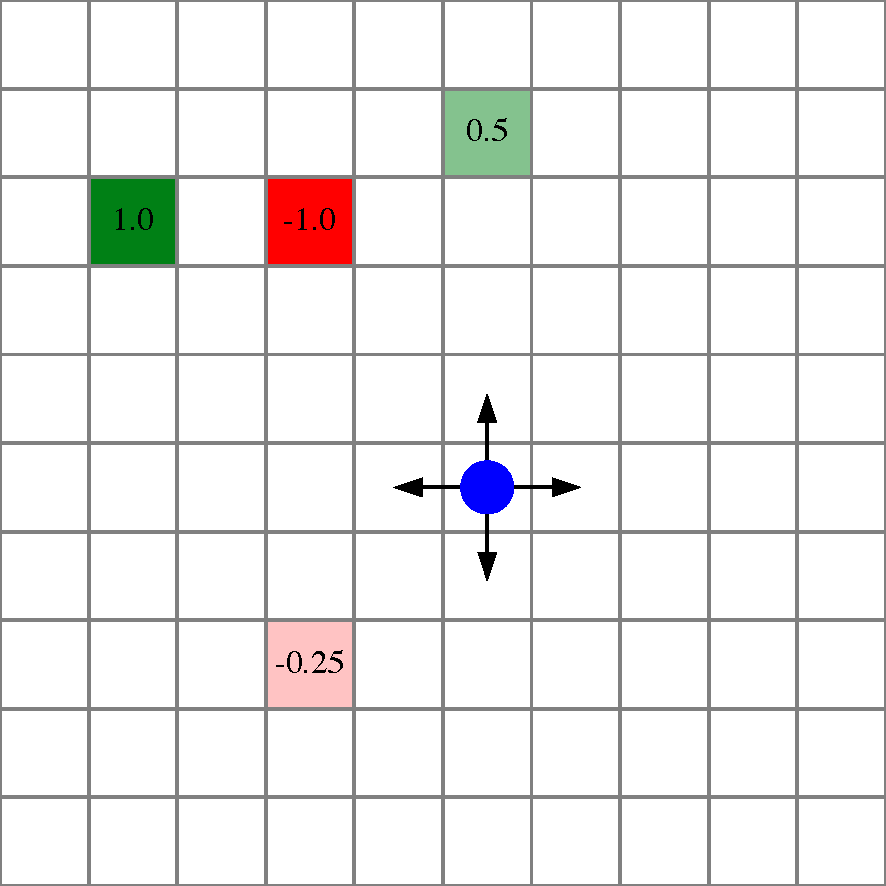
\includegraphics[width=0.5\textwidth]{figures/sample_systems/simple_gridworld.pdf}
    \caption{Simple Gridworld MDP.}
    \label{fig:simple_gridworld}
\end{figure}

% Adversarial MDP
The adversarial version of the simple gridworld is described by the failure condition, disturbance space, and disturbance model.  We define a failure as any time the agent reaches a terminal state with negative reward. The disturbances are the stochastic transitions of the agent so the disturbance space is the same as the action space of the base MDP: [\emph{up}, \emph{down}, \emph{left}, \emph{right}]. The probability of a disturbance is in state $s$ is
\begin{equation}
    p(x \mid s) = \begin{cases}
    p_{\rm success} & \text{if } x = \pi(s) \\
    (1 - p_{\rm success}) / 3 & \text{if } x \neq \pi(s) \\ 
    \end{cases}
\end{equation}
The reward function and discount factor are task and solver dependent and will be discussed in the description of the safety validation experiments. 

% Implementation details
The implementation of both the base and adversarial MDP can be done using the \texttt{SimpleGridworld} MDP distributed as part of the POMDPModelTools.jl\footnote{https://github.com/JuliaPOMDP/POMDPModelTools.jl} package. The base MDP can be implemented by defining the grid size, the value and location of the rewards, the states to terminate from, and the probability of a successful transition. The adversarial MDP can then be constructed with the same size and terminal states, but the rewards are now set to \num{1} for each failure state in the base MDP, and \num{0} for all others. The probability of transition success is set to \num{1} so that the actions of the adversarial MDP completely control the agent.



\subsection{Gridworld with Adversary}
% Base MDP
In order to increase the difficulty of the safety validation problem we introduce a new gridworld variation that includes an adversarial agent (shown in \cref{fig:gridworld_with_adversary}). Two agents move on an $N_x \times N_y$ gridworld: the ego agent (in blue) tries to reach states with high reward, while the adversary (in orange) tries to collide with the ego agent. The state of the environment is the grid location of each agent and the action space is [\emph{up}, \emph{down}, \emph{left}, \emph{right}, \emph{stay}, \emph{up-right}, \emph{up-left}, \emph{down-right}, \emph{down-left}], which control the transitions of the ego agent. For each episode the agents are initialized to a random non-terminal position. On each iteration both agents select an action and then transition to the corresponding cell with probability $p_{\rm success}$, or to another adjacent cell with probability $1-p_{\rm success}$. Some states are marked as impassible (shown in black), so if the agent would transition to an impassible state or out of bounds of the gridworld then it stays in its current state. The episode terminates when the ego agent reaches a terminal state (any state with positive reward) or the two agents overlap in the same state. The state space of this MDP is the square of the simple gridworld, but for modestly sized grids, dynamic programming is tractable for solving for the optimal ego policy. 

\begin{figure}
    \centering
    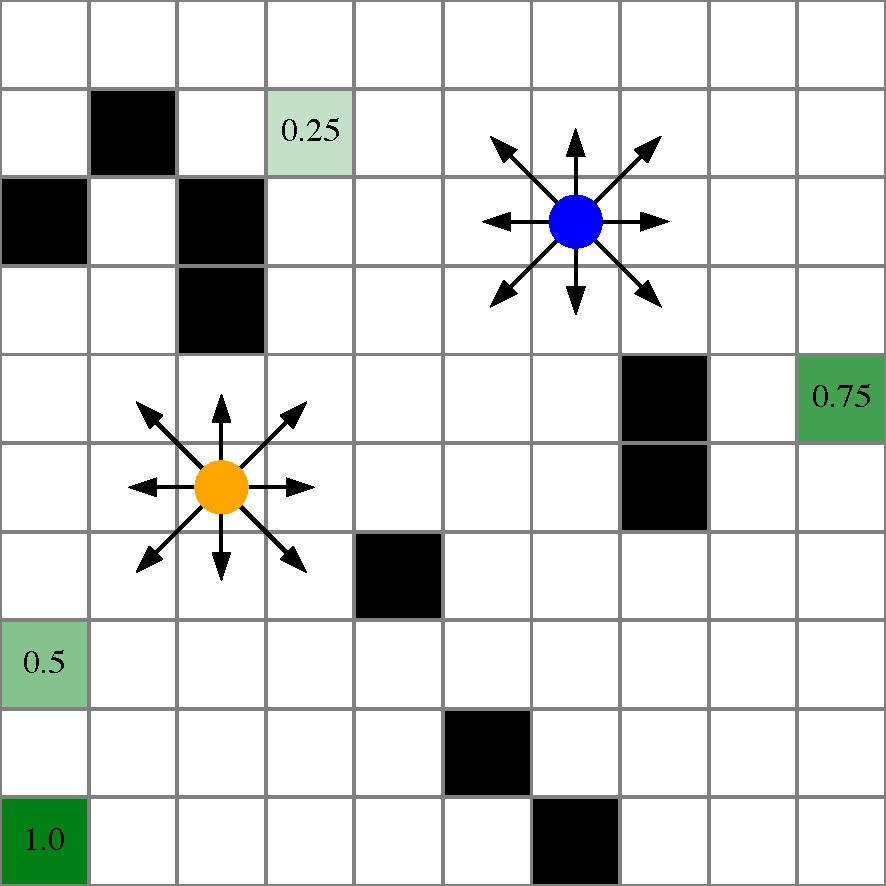
\includegraphics[width=0.5\textwidth]{figures/sample_systems/gridworld_with_adversary.pdf}
    \caption{Gridworld with Adversray MDP.}
    \label{fig:gridworld_with_adversary}
\end{figure}

For the adversarial MDP, we define a failure of the ego agent as a collision between the ego agen and the adversary. The disturbances are the actions of the adversarial agent and so the disturbance space is the same as the action space in the base MDP. The probability of each disturbance can be user specified. If we assume that the adversary moves entirely at random, then the probability of each disturbance would be $p(x \mid s) = 1 / 9$.

Both the base MDP and the adversarial MDP can be implemented using the julia package AdversarialGridworld.jl\footnote{https://github.com/sisl/AdversarialGridworld.jl}. A gridworld with an adversary is defined by specifying the grid size, the location of terminal states, the rewards, and the location of impassible states and the probability of successful transitions $p_{\rm success}$. The MDP can be switched between base mode and adversarial mode. In base mode, the actions of the MDP correspond to the actions of the ego agent and the reward function returns positive reward when the ego agent reaches a reward state and negative reward for a collision. In adversarial mode, the actions of the MDP correspond to the adversary and the reward function gives a positive reward for collisions. In both modes, the agent that is not controlled by the actions of the MDP must have a policy associated with it.

\section{Autonomous Driving}
% Why autonomous vehicles
To complement the simplicity of the gridworld MDPs, we introduce two MDPs to model autonomous driving behavior in complex environments. Autonomous driving is an especially important domain for safety validation due to the recent development and deployment of autonomous vehicles~\cite{koopman2016challenges}. Safety validation of an autonomous driving policy is challenging due to the size of the state and disturbance spaces, the duration of the diving episodes, and the rarity of failure events.

% How we model driving and adversarial driving MDPs
To model driving scenarios in simulation we build off of the julia package AutomotiveSimulator.jl\footnote{https://github.com/sisl/AutomotiveSimulator.jl} which provides methods for constructing road geometries, vehicles, pedestrians and behavior models. To facilitate the construction of adversarial MDPs for driving scenarios, we developed the package AdversarialDriving.jl\footnote{https://github.com/sisl/AdversarialDriving.jl}. Adversarial driving scenarios are constructed from a set of agents where each agent is defined by
\begin{itemize}
    \item An \emph{initialization function} that generates the initial state of the agent. The function may be deterministic or randomized, and is called each time the MDP is reset. 
    \item A \emph{behavior model} that determines the actions of the agent. For the system under test, the behavior model implements the autonomous driving policy we wish to test. For adversaries, the model implements their behavior and disturbances.
    \item A \emph{disturbance model} that is a probability distribution over disturbances which can be used to sample disturbances and compute their probability. 
\end{itemize}

% Description of the state space, action space, and  dynamics
The MDP is constructed with an agent representing the system (called the ego vehicle), a vector of agents that act as the adversaries (either other vehicles or pedestrians), a road geometry, and the simulation timestep. The state and action spaces are dynamically constructed based on the number and type of agents in the scene. We assume that vehicles stay in their lane during the simulation and can therefore specify a vehicle's state using four state variables ($r$, $v$, $\ell$, $b$) where $r$ is the position along the lane, $v$ is the speed of the vehicle in the direction of the lane, $\ell$ is an integer representing which lane the vehicle is in, and $b$ is a Boolean that indicates if the vehicle's turn signal is on. Pedestrians can move in any direction so their state is described by two position and two velocity variables ($r_x$, $r_y$, $v_x$, $v_y$). At each step, vehicles can apply an acceleration in the direction of the direction of the lane and pedestrians can apply a 2D acceleration. The position and velocity of each agent (in each direction) is updated by the kinematic relation
\begin{equation}
\begin{split}
    r_{t+\Delta t} &= r_t + v_t \Delta t + \frac{1}{2} a_t \Delta t^2 \\
    v_{t+\Delta t} &= v_t + a_t \Delta t
    \end{split}
    \label{eq:kinematics}
\end{equation}
where $\Delta t$ is the simulation timestep. Additionally, vehicles that have the opportunity to make a turn can toggle their intention to turn and whether or not their turn signal is on. The policies we use to control agents in the scene are Markov, so the simulation can be initialized into an arbitrary state.


% Description of the intelligent driving model
The driving policy that we use for vehicles is based on the intelligent driver model (IDM), a rule-based algorithm that applies longitudinal acceleration to reach a desired velocity while avoiding rear-end collisions. The IDM algorithm is shown in \cref{alg:idm}. It takes as input the current separation between the ego vehicle and the agent ahead of it $\Delta s$, the velocity of the ego $v_{\rm ego}$, and the velocity of the lead vehicle $v_{\rm lead}$. If there is no lead vehicle then $\Delta s = \infty$ and $v_{\rm lead} = {\rm NaN}$. In the presence of a leading vehicle (line \ref{line:idm_has_lead}), the IDM computes a desired following distance (line \ref{line:idm_compute_desired}) and then computes an acceleration to match the desired velocity and following distance (line \ref{line:idm_compute_acc}). If there is no leading vehicle (line \ref{line:idm_nolead}) then the acceleration is computed to gradually approach the desired driving velocity (line \ref{line:idm_compute_acc_free}). The behavior of the IDM is governed by a set of driving parameters which are shown in \cref{tab:idm_params} with their default values. 


\begin{table}
    \centering
    \caption{Default IDM parameter values.}
    \label{tab:idm_params}
    \begin{tabular}{@{}lll@{}} 
        \toprule
        \textbf{Description} & \textbf{Variable} & \textbf{Default Value} \\
        \midrule
        Speed tracking constant & $k$ & \SI{1.0}{s^{-1}} \\
        Acceleration exponent & $\delta$ & \num{4.0} \\
        Desired time headway & $T_{\rm des}$ & \SI{1.5}{s}\\
        Minimum allowed gap & $r_{\rm min}$ & \SI{5.0}{m} \\
        Desired velocity & $v_{\rm des}$ & \SI{15.0}{m/s} \\
        Maximum acceleration & $a_{\rm max}$ & \SI{3.0}{m/s^2} \\
        Comfortable deceleration & $d_{\rm comf}$ & \SI{2.0}{m/s^2} \\
        Maximum deceleration & $d_{\rm max}$ & \SI{9.0}{m/s^2} \\
        \bottomrule
    \end{tabular}
    \vskip -0.2in
\end{table}


 \begin{algorithm}
\caption{Intelligent Driver Model.}
    \label{alg:idm}
\begin{algorithmic}[1]
    \Function{IDMAcceleration}{$\Delta r$, $v_{\rm ego}$, $v_{\rm lead}$}
    \State $\Delta v \gets v_{\rm lead} - v_{\rm ego}$
    \If{$v_{\rm lead} \neq \rm{NaN}$} \label{line:idm_has_lead}
        \State $r_{\rm des} = r_{\rm min} + v_{\rm ego} \Delta T_{\rm des} - \frac{v_{\rm ego} \Delta v}{2 \sqrt{a_{\rm max} d_{\rm comf}}}$ \label{line:idm_compute_desired}
        \State $a \gets a_{\rm max} \left( 1 - \left(\frac{v_{\rm ego}}{v_{\rm des}} \right)^{\delta} - \left( \frac{r _{\rm des}}{\Delta r} \right)^2 \right)$ \label{line:idm_compute_acc}
    \Else \label{line:idm_nolead}
        \State $a \gets k \Delta v$ \label{line:idm_compute_acc_free}
    \EndIf
    \State \textbf{return} \textproc{clamp}($a$, $-d_{\rm max}$, $a_{\rm max}$) \label{line:idm_clamp_acc}
    \EndFunction
\end{algorithmic}
\end{algorithm}


% Describe the intersection algorithm
The intelligent driving model works well for traffic on a single roadway, but is not designed to handle intersections. To allow the autonomous vehicle to navigate intersections we developed a rule-based intersection navigation algorithm that uses the IDM (shown in \cref{alg:intersection_navigation}). The algorithm takes as input the ego vehicle $veh$ that is being controlled, the $scene$ that contains the other agents on the road, and the $roadway$ which describes the road geometry. We first determine the velocity and relative position of any agent in the same lane as the ego vehicle (line \ref{line:intersectionidm_leading_vehicle}). 
If there is no leading vehicle, then the velocity will be $v_{\rm lead} = {\rm NaN}$ and the relative position will be infinite. We then check if the ego vehicle has right of way in the intersection (line \ref{line:intersection_if_ROW}), and if it does, the vehicle proceeds with the IDM acceleration (line \ref{line:intersection_regular_idm_acc}). The right of way rules are 1) vehicles going straight have priority over vehicles that are turning and 2) vehicles turning right have priority over vehicles turning left. If a vehicle has a turn signal on, them it is assumed to be turning and vice versa. 

If the vehicle does not have right of way then the distance to the intersection (line \ref{line:intersection_distance2intersection} and the time it will take to cross it (line \ref{line:intersection_timetocross}) are computed and used to determine if the intersection is occupied. The intersection is considered occupied if for any other agent on the road, that agent is already in the intersection or, based on its current velocity, will be in the intersection during the planned crossing time of the ego vehicle. If the intersection is occupied and the lead vehicle has already passed the intersection then we use the stationary boundary of the intersection as the reference point for the IDM (line \ref{line:intersection_idm2int}), and otherwise we use the leading vehicle still (line \ref{line:intersection_regular_idm_acc2}).


 \begin{algorithm}
\caption{Intersection navigation algorithm.}
    \label{alg:intersection_navigation}
\begin{algorithmic}[1]
    \Function{IntersectionIDMAcceleration}{$veh$, $scene$, $roadway$}
        \State $v \gets$ \textproc{Velocity}($veh$)
        \State $v_{\rm lead}$, $\Delta s_{\rm lead} \gets$ \textproc{LeadingVehicle}($veh$, $scene$) \label{line:intersectionidm_leading_vehicle}
        \If{\textproc{HasRightOfWay}($veh$, $scene$, $roadway$)} \label{line:intersection_if_ROW}
            \State \textbf{return} \textproc{IDMAcceleration}($\Delta s_{\rm lead}$, $v$, $v_{\rm lead}$) \label{line:intersection_regular_idm_acc}
        \Else
            \State $\Delta s_{\rm int} \gets$ \textproc{DistanceToIntersection}($veh$, $roadway$) \label{line:intersection_distance2intersection}
            \State $\Delta t_{\rm cross} \gets$ \textproc{TimeToCrossIntersection}($veh$, $roadway$)  \label{line:intersection_timetocross}
            
            \If{\textproc{IntersectionOccupied}($scene$, $roadway$, $\Delta t_{\rm cross}$) and $\Delta s_{\rm int} < \Delta s_{\rm lead}$} \label{line:intersection_occupied}
                \State \textbf{return} \textproc{IDMAcceleration}($\Delta s_{\rm int}$, $v$, \num{0}) \label{line:intersection_idm2int}
            \Else
                \State \textbf{return} \textproc{IDMAcceleration}($\Delta s_{\rm lead}$, $v$, $v_{\rm lead}$) \label{line:intersection_regular_idm_acc2}
            \EndIf
        \EndIf
    \EndFunction
\end{algorithmic}
\end{algorithm}

% Assumptions used for the intersection navigation algorithm
The intersection navigation algorithm relies on several assumptions to make it functional. For sensing, it assumes that the ego vehicle can noisily observe all other agents in the scene (no occlusions), and has perfect knowledge of the road geometry (such as the location of any intersections). For the behavioral modeling of other agents, it assumes that an agent will turn on its turn signal if and only if it is turning, and that other agents drive with a constant velocity when approaching the intersection. Any violation of these assumptions could lead to a collision. The goal of this driving policy, however, is not to build an industrial autonomous driving planner, but to construct a driving policy that exhibits complex driving behavior while avoiding most collisions. Weaknesses in the algorithm provide potential failure modes that we can investigate with the safety validation algorithms developed in later chapters. 

% Low fidelity simulation
The simulation environment is lower fidelity than simulators used in industry.  For example, the motion of the agents is controlled by point-mass dynamics instead of the complex 3D dynamics of a real vehicle or pedestrian. The environment is not rendered photo-realistically, so advanced perception systems cannot be used. The driving policy does not have machine-learned components and is assumed to be Markov. Despite these differences we have designed the autonomous driving scenarios to have similar state spaces, actions spaces, number of interacting agents and rarity of failure events to those of an industrial simulator and driving policy. Due to the this matching, we believe that safety validation algorithms that work for the following scenarios will be applicable to real-world autonomous driving simulators.


\subsection{Pedestrian in Crosswalk}
% Description of the base MDP
In the pedestrian crosswalk MDP shown in \cref{fig:pedestrian_crosswalk}, an autonomous vehicle approaches a crosswalk where a pedestrian is attempting to cross. The vehicle makes noisy observations of the pedestrian's position and velocity, and uses those observations with the intersection navigation algorithm (\cref{alg:intersection_navigation}) to determine its acceleration. Since there is only a single lane for the vehicle, the state space of the vehicle can be reduced to the longitudinal position and velocity ($r_x^{\rm veh}$, $v_x^{\rm veh}$) while the state of the pedestrian is the lateral and longitudinal position and velocity ($r^{\rm ped}_x$, $r^{\rm ped}_y$, $v^{\rm ped}_x$, $v^{\rm ped}_y$). The action space of the vehicle is the range of accelerations between $[-d_{\rm max}, a_{\rm max}]$. At the start of each episode, both agents are initialized randomly with the vehicle driving in the positive $x$-direction and the pedestrian is on the right side of the vehicle. At each step, both agents determine their accelerations and their position and velocity are updated according to the kinematic relations in \cref{eq:kinematics}. The episode ends if there is a collision between the vehicle and the pedestrian or if the vehicle makes it to the end of the roadway. Since the driving policy is rule-based and does not require any learning, we have no need to explicitly specify a reward for the base MDP. 

\begin{figure}
    \centering
    \begin{tikzpicture}
         \node (fig1) at (0,0)
           {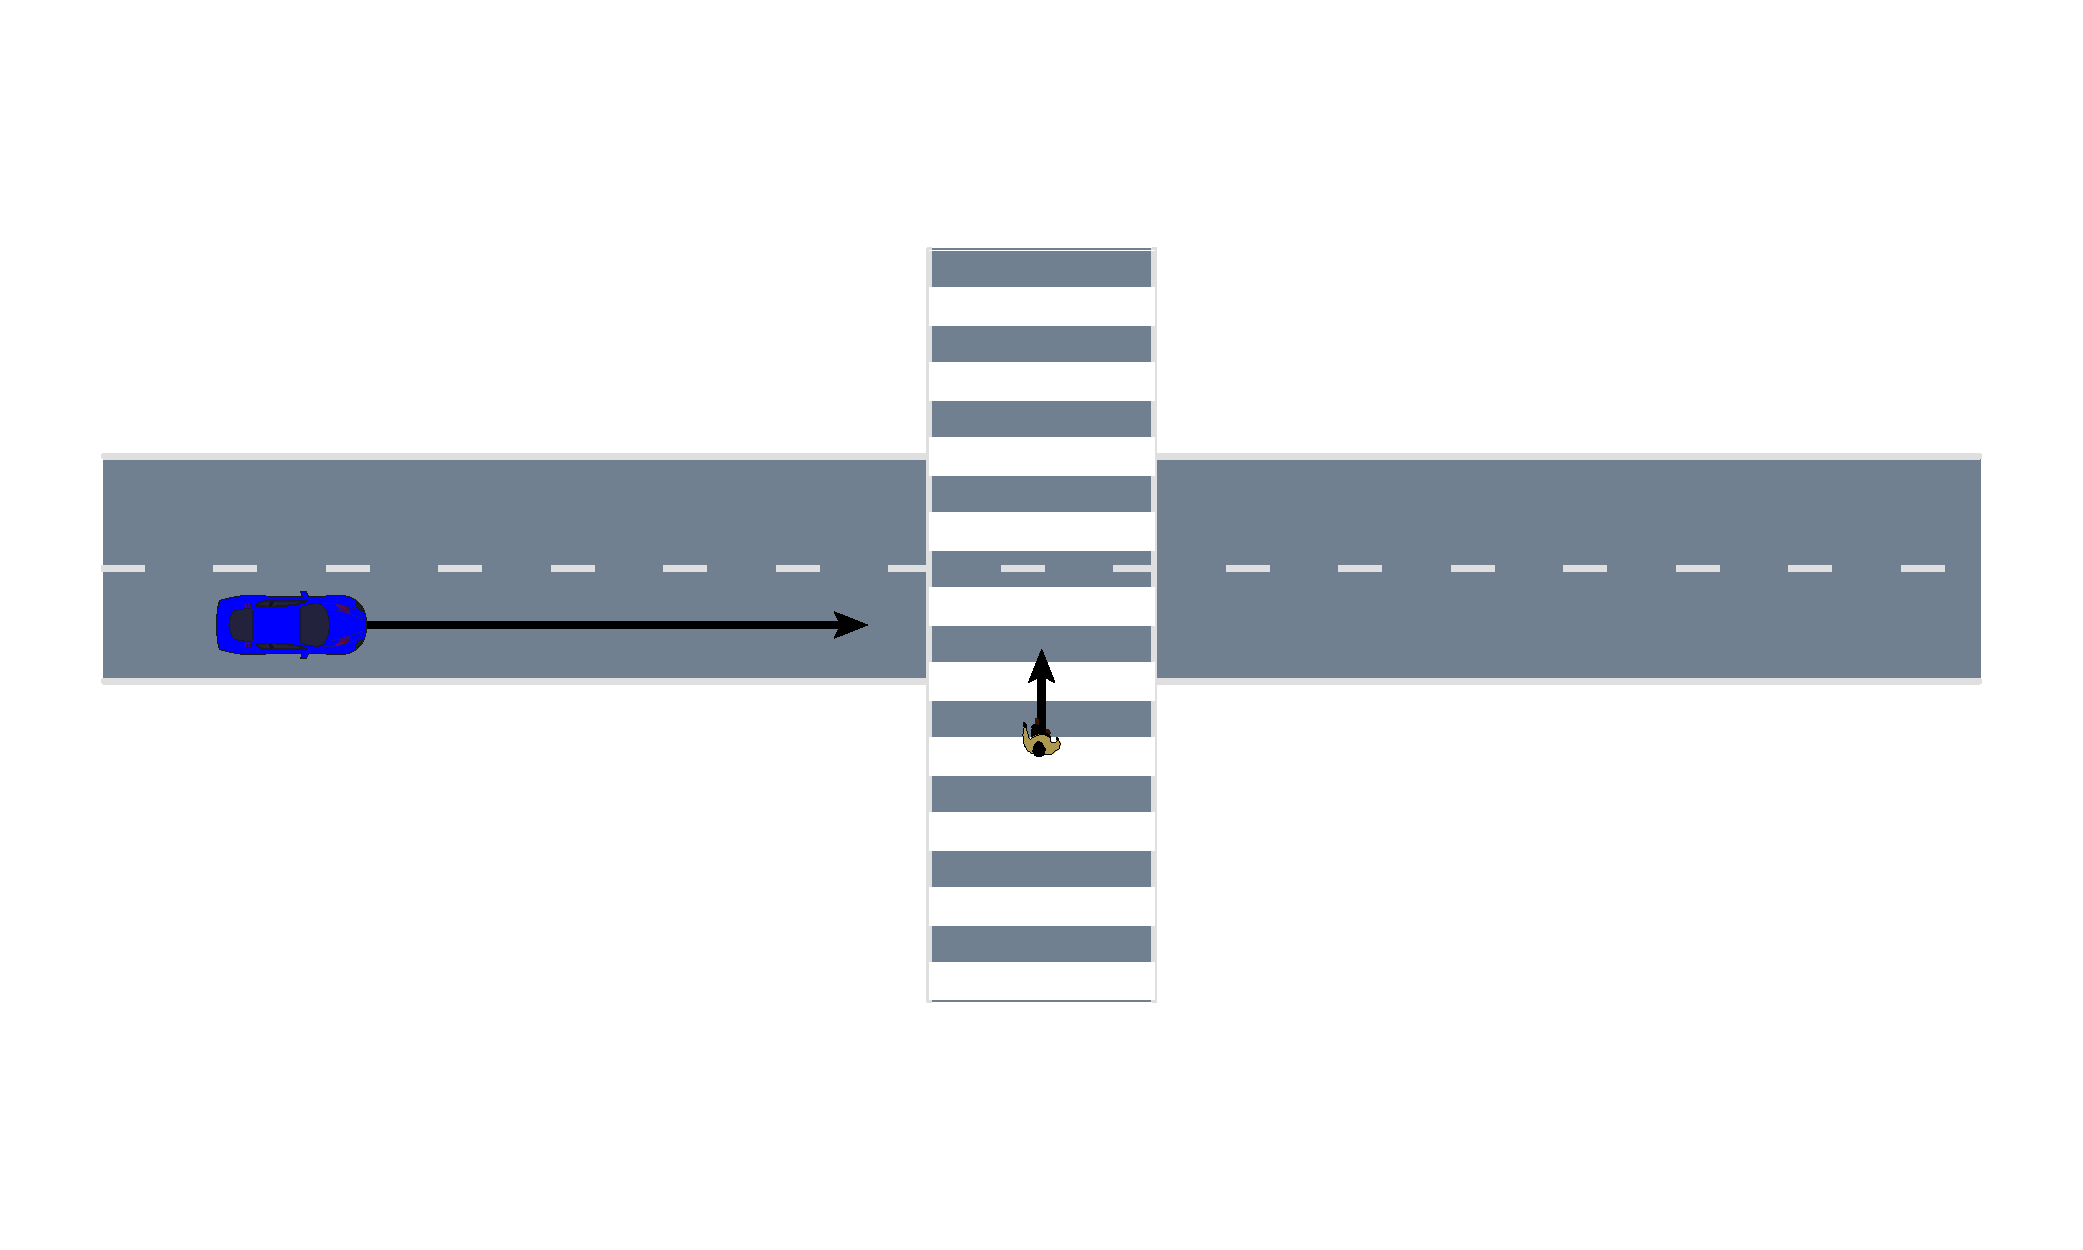
\includegraphics[trim={0 5cm 0 5cm},clip, width=\textwidth]{figures/sample_systems/pedestrian_crosswalk.pdf}};
         \draw[->] (5,-2.3)--(6,-2.3) node[right]{$x$};
         \draw[->] (5,-2.3)--(5,-1.4) node[above]{$y$};
    \end{tikzpicture}
    \caption{Crosswalk MDP where the ego vehicle approaches a crosswalk while a pedestrian tries to cross. }
    \label{fig:pedestrian_crosswalk}
\end{figure}


% Description of the adversarial MDP
Failures of this scenario are defined by any collision between the pedestrian and vehicle. The disturbances are the lateral and longitudinal accelerations of the pedestrian ($\delta a_x$ $\delta a_y$), and the lateral and longitudinal noise in the measurement of the pedestrian's position and velocity ($\delta n_x$, $\delta n_y$, $\delta n_v$). All five disturbances are continuous but if we are using a safety validation solver that requires a discrete disturbance space, then we can discretize them. If we assume that the disturbances are independent then we can model each with a zero-mean Gaussian distribution. If we want to model correlated disturbances to better caption human-like behavior, we can model them as Gaussian processes with kernel function $\vec{k}$ and mean function $\vec{\mu}$. These options are shown in \cref{tab:adversarial_ped_disturbance_space}.


\begin{table}
    \centering
    \caption{Continuous disturbance space for adversarial pedestrian in crosswalk MDP.}
    \label{tab:adversarial_ped_disturbance_space}
    \begin{tabular}{@{}lrr@{}} 
        \toprule
        \textbf{Disturbance} & \textbf{Independent} & \textbf{Correlated} \\
        \midrule
        Lateral Acceleration &  $\delta a_x \sim \mathcal{N}(0, \sigma_{a_x}^2)$ &  $\vec{\delta a}_x \sim \mathcal{N}(\vec{\mu}_{a_x}(\vec{t}), \vec{k}_{a_x}(\vec{t}, \vec{t}))$ \\
        Longitudinal Acceleration &  $ \delta a_y \sim \mathcal{N}(0, \sigma_{a_y}^2)$ &  $\vec{\delta a}_y \sim \mathcal{N}(\vec{\mu}_{a_y}(\vec{t}), \vec{k}_{a_y}(\vec{t}, \vec{t}))$ \\
        Lateral Position Noise &  $\delta n_x \sim \mathcal{N}(0, \sigma_{r_x}^2)$ &  $\vec{\delta n}_x \sim \mathcal{N}(\vec{\mu}_{r_x}(\vec{t}), \vec{k}_{r_x}(\vec{t}, \vec{t}))$ \\
        Longitudinal Position Noise &  $\delta n_y \sim \mathcal{N}(0, \sigma_{r_y}^2)$ &  $\vec{\delta n}_y \sim \mathcal{N}(\vec{\mu}_{r_y}(\vec{t}), \vec{k}_{r_y}(\vec{t}, \vec{t}))$ \\
        Velocity Noise &  $\delta n_v \sim \mathcal{N}(0, \sigma_{v}^2)$ &  $\vec{\delta n}_{v} \sim \mathcal{N}(\vec{\mu}_{v}(\vec{t}), \vec{k}_{v}(\vec{t}, \vec{t}))$ \\
        \bottomrule
    \end{tabular}
\end{table}
 



\subsection{T-Intersection}

% Base MDP
In the T-intersection MDP (shown in \cref{fig:t_intersection}), the ego vehicle tries to make an unprotected left turn onto a two-lane through-street with other vehicles at the intersection. The state of the $i$th vehicle is ($r_i$, $v_i$, $\ell_i$, $b_i$) where $r_i$ and $v_i$ are the position and velocity along lane $\ell_i$, and $b_i$ is a Boolean indicating if the vehicle's turn signal is on. The intersection is composed of \num{6} lanes: $\ell = 1$ is the lane that goes straight from left to right, $\ell = 2$ starts as lane \num{1} but turns right, $\ell = 3$ is the lane that goes straight from right to left, $\ell = 4$ starts as lane \num{3} but turns left, $\ell = 5$ turns left onto the through street, and $\ell = 6$ turns right onto the through street. Vehicles that are on the through-street can change their turn intention by changing their lane prior to the intersection. For example, a vehicle going straight in lane \num{1} can choose to turn right by switching to lane \num{2} before the turn. Each lane has at most one other lane that a vehicle could switch to without changing its position, so changing lanes can be considered an operation that toggles \emph{turn intention}.

At the start of each episode, the agents are randomly initialized into a configuration that would lead to no collisions in the absence of disturbances. On each step, each vehicle on the road makes observations of the other agents and uses \cref{alg:intersection_navigation} to determine their acceleration to safely travel through the intersection. The episode terminates when there is a collision between any two vehicles or when the ego vehicle successfully makes the left turn and reaches the end of the roadway. 

\begin{figure}
    \centering
    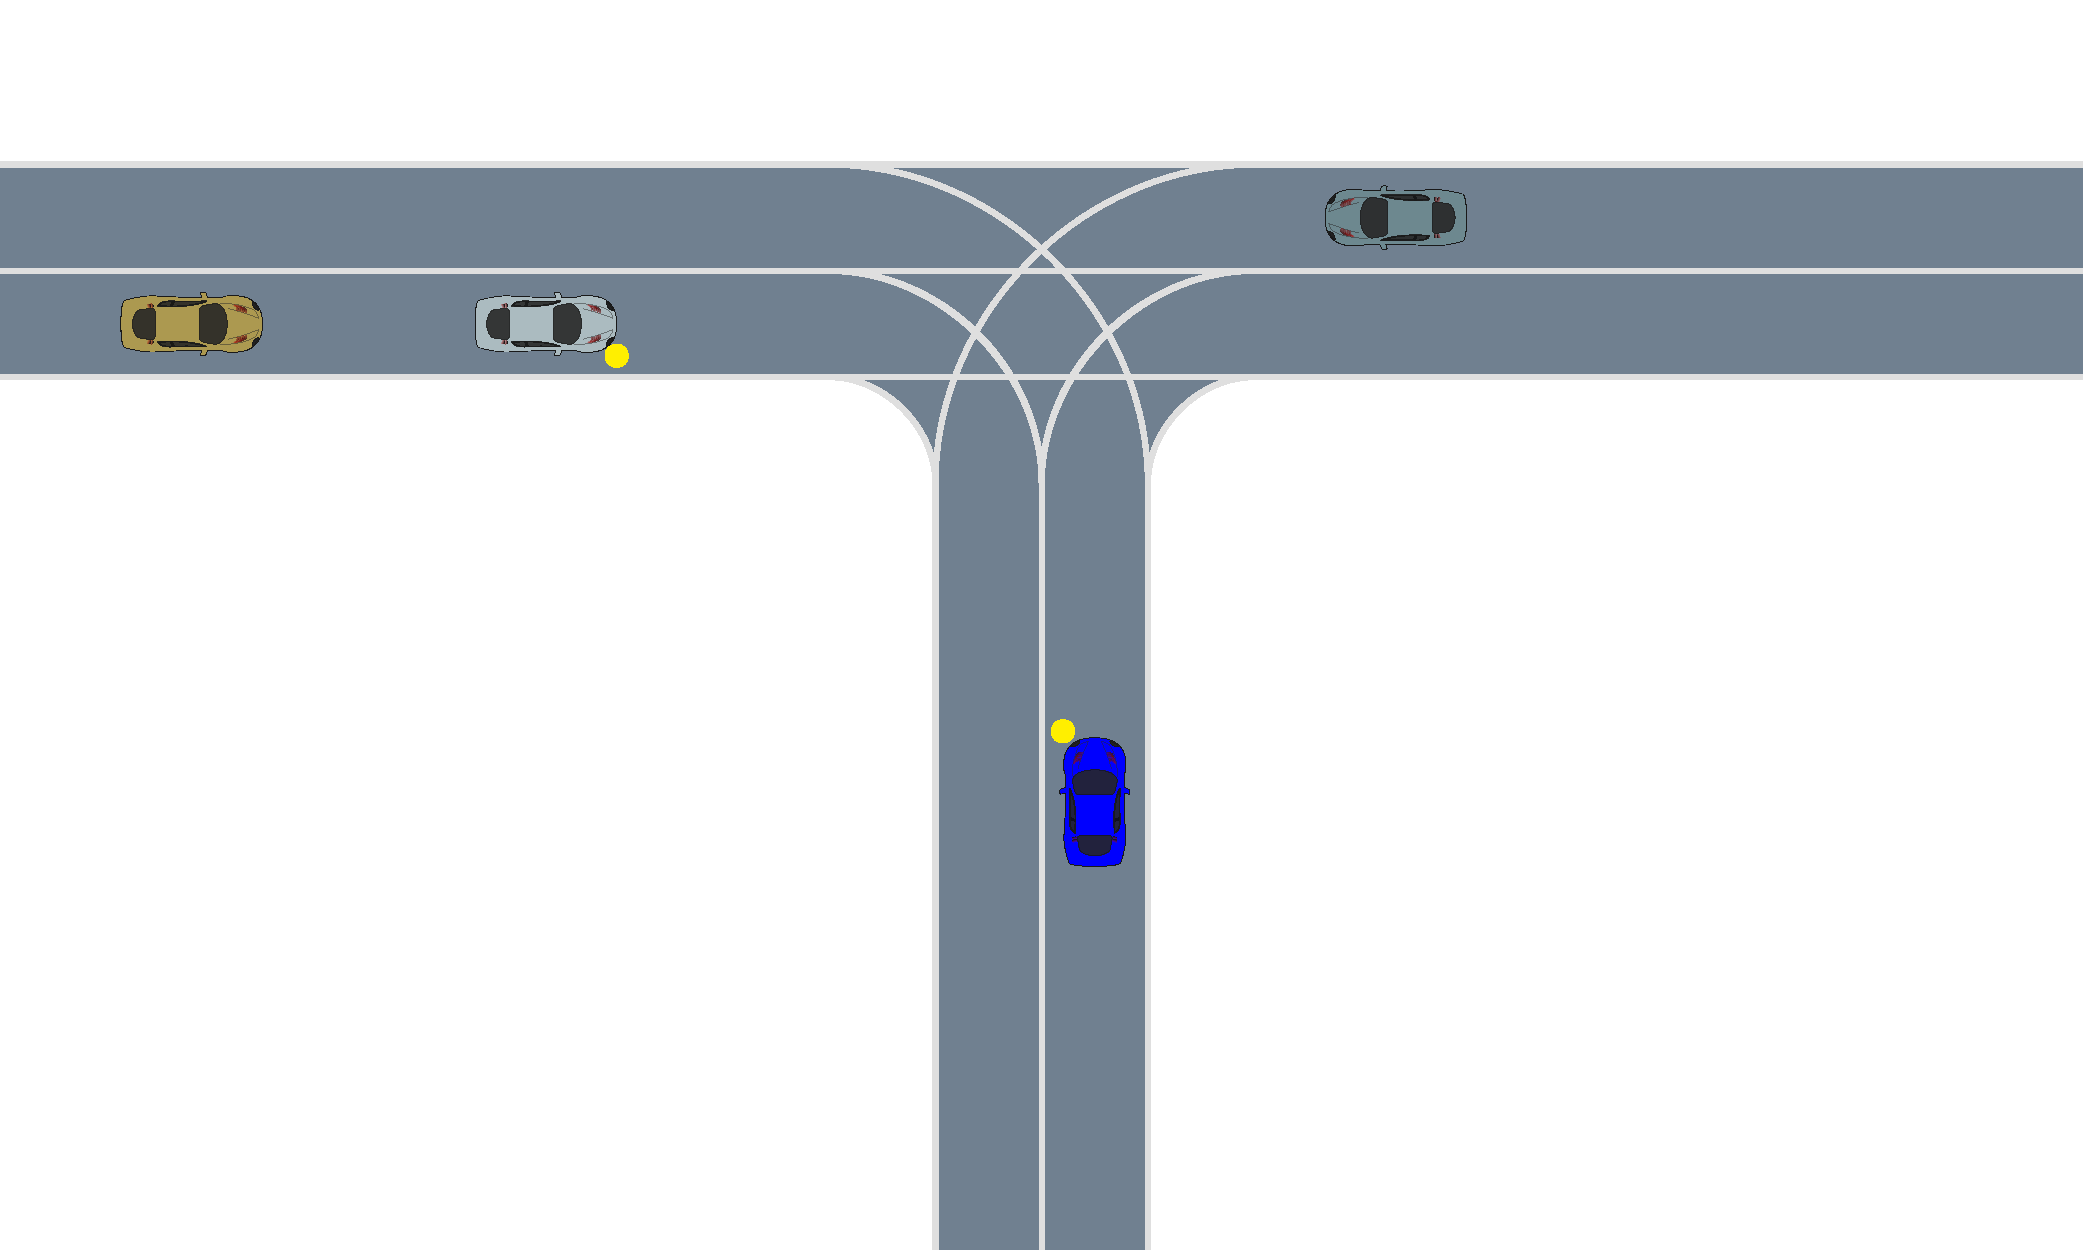
\includegraphics[trim={0 5cm 0 0},clip, width=\textwidth]{figures/sample_systems/T_intersection.pdf}
    \caption{T-Intersection MDP where the ego vehicle tries to take unprotected left turn. }
    \label{fig:t_intersection}
\end{figure}

% Adversarial MDP
In the adversarial MDP, a failure is any collision between the ego vehicle and another vehicle on the road. For each vehicle (other than the ego), the disturbances are perturbations to the vehicle's acceleration $\delta a$, toggling turn intention $\delta \ell$, or toggling the turn signal $\delta b$. If we treat the acceleration disturbance as continuous, then the disturbances can be modeled by the distributions shown in \cref{tab:Tint_continuous_disturbance_space}. If we require discrete disturbances then we can choose \num{7} representative disturbances and their associate probabilities as shown in \cref{tab:Tint_discrete_disturbance_space}.

\begin{table}
    \centering
    \caption{Continuous disturbance space for adversarial vehicles in T-intersection MDP.}
    \label{tab:Tint_continuous_disturbance_space}
    \begin{tabular}{@{}lrr@{}} 
        \toprule
        \textbf{Disturbance} & \textbf{Distribution} \\
        \midrule
        Acceleration &  $\delta a \sim \mathcal{N}(0, \sigma_a^2)$ \\
        Toggle turn intent & $\delta \ell \sim {\rm Bern}(\rho_I)$ \\
        Toggle turn signal & $\delta b \sim {\rm Bern}(\rho_S)$\\
        \bottomrule
    \end{tabular}
\end{table}

\begin{table}
    \centering
    \caption{Discrete disturbance space for adversarial vehicles in T-intersection MDP.}
    \label{tab:Tint_discrete_disturbance_space}
    \begin{tabular}{@{}lrr@{}} 
        \toprule
        \textbf{Disturbance} & \textbf{Acceleration} & \textbf{MC Probability} \\
        \midrule
        No disturbance &  \SI{0}{m/s^2} & \num{0.976}\\
        Medium slowdown & \SI{-1.5}{m/s^2} & \num{1e-2}\\
        Major slowdown & \SI{-3}{m/s^2} & \num{1e-3}\\
        Medium speedup & \SI{1.5}{m/s^2} & \num{1e-2}\\
        Major speedup & \SI{3}{m/s^2} & \num{1e-3}\\
        Toggle blinker & N/A & \num{1e-3 }\\
        Toggle turn intent & N/A & \num{1e-3} \\
        \bottomrule
    \end{tabular}
\end{table}

\section{Discussion}

In this chapter we introduced the idea of an adversarial MDP to model the safety validation of an autonomous policy for a base MDP. Both MDPs share the same state space and transition model, but the actions of the base MDP are the actions of the system while the actions of the adversarial MDP are the disturbances. The adversarial MDP is a flexible model that can be used in conjunction with safety validation algorithms based on optimization, path-planning, reinforcement learning, and importance sampling.

We then introduced four safety validation problems that are used to test the safety validation algorithms developed in the remainder of this thesis. The first scenario involves the safety validation of a simple gridworld policy where the disturbances are the stochastic transitions of the agent. The second scenario is also a gridworld problem, but with another adversarial agent that causes collisions. The next two systems model autonomous driving scenarios. In the first, the ego vehicle approaches a crosswalk with a crossing pedestrian and must avoid the pedestrian under disturbances to the pedestrian motion and sensor noise. The second driving scenario is a T-intersection where the ego vehicle makes an unprotected left turn onto a through-street with other drivers on the road. The disturbances are the behavior of other vehicles on the road and include perturbations to the acceleration, toggling of turn intention and toggling the turn signal.

The following chapter begins the development of safety validation algorithms. We introduce a technique for interpretable safety validation and demonstrate it with the autonomous driving scenarios. 

\chapter{Interpretable Safety Validation}
In this chapter, we develop an algorithm for interpretable safety validation that generates failure descriptions in the form of signal temporal logic expressions. A failure description is any statement that defines a set of disturbance trajectories that cause the system to fail and is useful for understanding failure modes, producing failure examples. Failure descriptions are found using expression optimization and evaluated by sampling satisfying trajectories. We introduce a technique for sampling satisfying trajectories of STL specifications by applying a set of linear constraints to the disturbance model which can be done efficiently for independent disturbances and disturbances that are jointly distributed as a Gaussian process. Through experiments in two autonomous driving scenarios, we demonstrate that our interpretable safety validation algorithm can find failure descriptions, and produce a diverse set of failure examples. Failure descriptions may also be used to analyze the sensitivity of the safety of the system with respect to important disturbance parameters. 

\section{Motivation}

% Introduce the problem (motivation)
One of the drawbacks to black-box safety validation techniques approaches is that they do not produce high-level descriptions of failures and instead only produce high-dimensional failure examples. In scenario-based testing, by contrast, each scenario involves semantically similar disturbance trajectories which can provide clues to the source of an error. For example, suppose a black-box safety validation algorithm discovered a failure of an autonomous vehicle driving on the highway. It would not be clear from this one example if the failure was due to perception, planning, control or something else. If, however, we found that the vehicle failed in a scenario designed to test its response to partially occluded stop signs, we would be justified in investigating the perception system. This work tries to bring a greater degree of interpretability to black box safety validation algorithms. 

% The approach we propose
Our approach seeks to find a \emph{failure description} $\varphi$ such that any disturbance trajectory that satisfies the description will cause the system to fail. For falsification, we want to find any such $\varphi$ where
\begin{equation}
    \vec{x} \in \varphi \implies f(\vec{x}) \not \in \psi \text{.}
\end{equation}
For most likely failure analysis we want to find the $\varphi$ that produces failures with high likelihood
\begin{equation}
\max_\varphi \quad \mathbb{E}_{\vec{x} \sim p(\vec{x} \mid \vec{x} \in \varphi)}[p(\vec{x})] \quad\textrm{s.t.}\quad \vec{x} \in E
\end{equation}
where $p(\vec{x} \mid \vec{x} \in \varphi)$ is the probability density of disturbance trajectories that satisfy the description. 

A failure description $\varphi$ contains more information than a single failure example. For example, a single failure description can produce many failure examples by sampling from $p(\vec{x} \mid \vec{x} \in \varphi)$. It also identifies logical features of a disturbance trajectory that are sufficient to cause a failure. As in scenario-based testing, those features may provide clues to the source of the error in the system. Lastly, if the features are low dimensional, they can be used to perform a sensitivity analysis of the safety of the system with respect to the disturbance variables. 


\section{STL Expression Optimization}
This section provides the necessary technical background to understand our approach for STL expression optimization. We first introduce context free grammars as a way to compactly represent signal temporal logic and describe how to sample valid STL expressions. We then describe genetic programming, a technique used to optimize tree-like structures such as STL expressions. Lastly, we introduce the failure description cost function that is used to find optimal failure descriptions.

\subsection{Context-Free Grammars}
\begin{figure}
    \centering
    \begin{forest}{for tree={ minimum size=1cm,}}
        [$\square$ 
            [$t_1$] 
            [$t_2$] 
            [$>$ 
                [$x$]
                [$0$]
            ]
        ]
    \end{forest}
    \caption{Expression tree for $\square_{[t_1, t_2]} x > 0$.}
    \label{fig:stl_tree}
\end{figure}

% Describing expressions as trees and grammar as a set of constraints
Logical expressions can be represented by a tree of symbols and operators. For example, the STL expression
\begin{equation}
    \square_{[t_1, t_2]} x > 0 \label{eq:example_stl_expression}
\end{equation}
can be represented by the tree shown in \cref{fig:stl_tree}. The semantics of a formal language specify a set of constraints on space of possible expression trees. These constraints can be compactly represented using a context-free grammar, which is a collection of production rules of the form
\begin{equation}
\mathbb{T} \mapsto \alpha,
\end{equation}
where $\mathbb{T}$ is a type and $\alpha$ is an expression that consists of types and symbols. A terminal production rule is one where $\alpha$ consists only of symbols. 

For example, the context-free grammar for a simplified version of STL for a single disturbance variable $x$ is given by
\begin{equation}
\label{eq:stl_grammar}
\begin{split}
    \mathbb{B} &\mapsto \mathbb{B} \land \mathbb{B} \mid \mathbb{B} \lor \mathbb{B} \mid \neg \mathbb{B} \mid \square_{[\mathbb{T},\mathbb{T}]}(\mathbb{S}) \mid \lozenge_{[\mathbb{T},\mathbb{T}]}(\mathbb{S}) \\
    \mathbb{T} &\mapsto 0:t_{\max} \\
    \mathbb{S} &\mapsto \mathbb{S} \land \mathbb{S} \mid \mathbb{S} \lor \mathbb{S} \mid \neg \mathbb{S} \mid x \leq \mathbb{X} \mid x \geq \mathbb{X} \mid x = \mathbb{X} \\
    \mathbb{X} &\mapsto [x_{\min},x_{\max}]
\end{split}
\end{equation}
The type $\mathbb{B}$ is used for Boolean scalars, $\mathbb{S}$ is for Boolean series, $\mathbb{T}$ is for time, and $\mathbb{X}$ is for values of $x$. The logical operators apply element-wise on series. The symbol $\mid$ separates rules on the same line and $:$ indicates a range of symbols. In this work, time is discrete and the variable $x$ may be discrete or continuous. When $x$ is continuous, $\mathbb{X}$ is sampled uniformly at random in the range $[x_{\min}, x_{\max}]$.

To generate an expression from a context-free grammar, we start by declaring the type of the desired expression and choose a production rule for that type. For example, if we want a valid STL, expression we start with the type $\mathbb{B}$ and select a rule from the first line of \cref{eq:stl_grammar}. Then, for each type in the expression, we expand it using a compatible production rule. The process recurses until all types have been expanded by terminal production rules and the expression contains only symbols. To construct \cref{eq:example_stl_expression} we applied the production rules
\begin{align}
    \mathbb{B} &\mapsto \square_{[\mathbb{T},\mathbb{T}]}(\mathbb{S}) \\
    \mathbb{T} &\mapsto t_1 \\
    \mathbb{T} &\mapsto t_2 \\
    \mathbb{S} &\mapsto x \leq \mathbb{X} \\
    \mathbb{X} &\mapsto 0 \text{.}
\end{align}
The selection of production rules can be done according to any distribution but it is common to choose them uniformly at random which favors shorter expressions~\cite{kochenderfer2019algorithms}. To implement grammars and expression sampling we use the package ExprRules.jl.\footnote{https://github.com/sisl/ExprRules.jl}


%%%%%%%%%%%%%%%%%%%%%%%%%%%%%%%%%%%%%%%%%%%%%%%%%%%%%%%%%%%%%%%%%%%%%%%%%%%%%%%%%%%%%%%%%%%%%%%%%%%%%%
\subsection{Genetic Programming}
\label{subsec:gp}
Genetic programming~\cite{kochenderfer2019algorithms, koza1992genetic} is a population-based optimization technique for expression trees that mimics the biological process of evolution. The algorithm (\cref{alg:genetic_programming}) takes as input a grammar $\mathcal{G}$, an expression cost function $c_\varphi$, and a population size $M$. To start, a population of $M$ expressions (or \emph{individuals}) is sampled from the grammar $\mathcal{G}$ (line \ref{line:gp_sample_pop}) using a uniform distribution over production rules. On each iteration, the cost of each expression is computed (line \ref{line:gp_compute_cost}) and used to select parents for reproduction (line \ref{line:gp_select}). The parents reproduce through a crossover operation to create a new population of $M$ children (line \ref{line:gp_select}). Then, some individuals are mutated to add new subtrees into the population (line \ref{line:gp_mutate}). Once the computational budget is exhausted, the individual with the lowest cost is returned (line \ref{line:gp_return}). We use the implementation of genetic programming from the ExprOptimiation.jl\footnote{https://github.com/sisl/ExprOptimization.jl} package.

\begin{algorithm}
\caption{Genetic programming.} \label{alg:genetic_programming}
\begin{algorithmic}[1]
    \Function{GeneticProgramming}{$\mathcal{G}$, $c_\varphi$, $M$}
    \State  $\vec{\varphi} \gets [\varphi_1, \ldots, \varphi_M]$ with  $\varphi_i \sim \mathcal{G}$ \label{line:gp_sample_pop}
    \Loop
        \State $\vec{c}_\varphi \gets [c_\varphi(\varphi_1), \ldots, c_\varphi(\varphi_M)]$ \label{line:gp_compute_cost}
        \State $(\vec{\varphi}_1, \vec{\varphi}_2) \gets \textproc{Select}(\vec{\varphi}, \vec{c})$ \label{line:gp_select}
        \State $\vec{\varphi} \gets \textproc{Crossover}(\vec{\varphi}_1, \vec{\varphi}_2))$ \label{line:gp_crossover}
        \State $\vec{\varphi} \gets \textproc{Mutate}(\vec{\varphi})$ \label{line:gp_mutate}
    \EndLoop
    \State \textbf{return} $\min_\varphi [c_\varphi(\varphi_1), \ldots, c_\varphi(\varphi_M)]$ \label{line:gp_return}
    \EndFunction
\end{algorithmic}
\end{algorithm}


\paragraph{Selection.} The selection procedure is designed to favor individuals with high \emph{fitness}. The fitness of an individual $\varphi_i$ is inversely related to its cost and can be computed as $\max \vec{c}_\varphi - c_\varphi(\varphi_i)$ where $\max \vec{c}_\varphi$ returns the largest cost in the population and $c_\varphi(\varphi_i)$ is the cost of individual $i$. Selection can be done using:
\begin{itemize}
    \item \emph{Truncation selection}: Parents are sampled uniformly at random from the $M$ fittest individuals.
    \item \emph{Tournament selection}: Each parent is the fittest individual of a randomly sampled subpopulation.
    \item \emph{Fitness-proportionate selection}: Parents are chosen with probability proportional to their fitness.
\end{itemize}

\paragraph{Crossover.} Crossover is way of constructing a new tree that has attributes of two parent trees. The procedure is shown in \cref{fig:gp_crossover}. A random node is selected in the first parent and replaced by a random subtree of the second parent. Care must be taken to ensure type-compatibility when making the exchange. 


\begin{figure}
    \centering
    \begin{subfigure}[t]{0.31\textwidth}
    \centering
    \begin{forest}{ for tree = {fill=white, draw=black, s sep+=1em, l-=3em}}
     [
            [[] []] 
            [] 
            [ , double, thick,
                []
                []
            ]
        ]
    \end{forest}
    \caption{Parent 1}
    \end{subfigure}
    \hfill
    \begin{subfigure}[t]{0.31\textwidth}
    \centering
    \begin{forest}{ for tree = {fill=black!30, draw=black, s sep+=1em, l-=3em}}
     [
            [[]] 
            [ , double, thick,
                []
                []
                []
            ]
        ]
    \end{forest}
    \caption{Parent 2}
    \end{subfigure}
     \hfill
    \begin{subfigure}[t]{0.31\textwidth}
    \centering
    \begin{forest}{ for tree = {fill=white, draw=black, s sep+=1em, l-=3em}}
     [
            [[] []] 
            [] 
            [ , fill=black!30
                [, fill=black!30]
                [, fill=black!30]
                [, fill=black!30]
            ]
        ]
    \end{forest}
    \caption{Child}
    \end{subfigure}
    \caption{Crossover operation that creates a child from two parents by replacing the highlighted subtree of parent one with the highlighted subtree of parent 2.}
    \label{fig:gp_crossover}
\end{figure}


\paragraph{Mutation.} Trees experience random mutations in order to introduce new features into the population. Mutation is demonstrated in \cref{fig:gp_mutation}. A random node in the tree is selected and replaced with a new expression of the same type sampled from the grammar. 


\begin{figure}
    \centering
    \begin{subfigure}[t]{0.31\textwidth}
    \centering
    \begin{forest}{ for tree = {fill=white, draw=black, s sep+=1em, l-=3em}}
         [
            [[]] 
            []
        ]
    \end{forest}
    \caption{Before Mutation.}
    \end{subfigure}
    \begin{subfigure}[t]{0.31\textwidth}
    \centering
    \begin{forest}{ for tree = {fill=white, draw=black, s sep+=1em, l-=3em}}
    [
            [[]] 
            [ , fill=black!30
                [, fill=black!30]
                [, fill=black!30]
                [, fill=black!30]
            ]
        ]
    \end{forest}
    \caption{After Mutation.}
    \end{subfigure}
    \caption{Mutation operation replaces a subtree with a randomly generated tree.}
    \label{fig:gp_mutation}
\end{figure}


\subsection{Failure Description Cost Functions}
A cost function for finding STL expressions that describe failure trajectories is shown in \cref{alg:failure_description_cost_function} which takes as input an STL expression $\varphi$ and returns the average safety metric of $N$ disturbance trajectories that satisfy $\varphi$. We first check if the description is satisfiable (line \ref{line:fdcost_is_satisfiable}) in case we sample a logically inconsistent expression such as $\square (x \geq 1 \land x \leq -1)$. In practice, we assume that an expression is not satisfiable if the sampling procedure fails to produce valid samples, in which case we return the maximal cost value $c_{\rm max}$ (line \ref{line:fdcost_return_max_cost}). Otherwise, we obtain $N$ disturbance trajectories that satisfy $\varphi$ (line \ref{line:fdcost_sample_disturbance_trajectory}) and use them to estimate the expected value of the safety metric from the average. Lastly, we add a penalty term (with parameter $\lambda$) for the number of nodes in the tree to ensure that expressions remain parsimonious (line \ref{line:fdcost_compute_avg}).

If the specification $\varphi$ is a failure description then trajectories that satisfy it should have a low value of the safety metric and lead to low cost, while the opposite is true if $\varphi$ has nothing to do with failures of the system. Therefore when $c_\varphi$ is used for optimization it should produce descriptions that frequently produce failure trajectories. If the probability is incorporated into $c(\vec{x})$ (as in \cref{eq:piecewise_cost}), then the optimization procedure will produce a failure description of the most likely failure modes. The most challenging part of computing the cost, however, is the need to sample trajectories that satisfy a given specification, which is the topic of the next section.

\begin{algorithm}
\caption{Failure description cost function.} \label{alg:failure_description_cost_function}
\begin{algorithmic}[1]
    \Function{$c_\varphi$}{$\varphi$}
    \If{\textproc{IsSatisfiable}($\varphi$)} \label{line:fdcost_is_satisfiable}
        \For{$i$ in $1:N$}
            \State Sample $\vec{x}_i$ from $p(\vec{x})$ s.t. $\vec{x} \in \varphi$ \label{line:fdcost_sample_disturbance_trajectory}
        \EndFor
        \State \textbf{return} $\frac{1}{N} \sum_{i=1}^N  c(\vec{x}_i) + \lambda \textproc{NodeCount}(\varphi)$ \label{line:fdcost_compute_avg}
        
    \Else
        \State \textbf{return} $c_{\rm max}$ \label{line:fdcost_return_max_cost}
    \EndIf
    \EndFunction
\end{algorithmic}
\end{algorithm}


\section{STL Satisfaction}
%todo:np hardness of satisfying stl statements?
A crucial piece of using expression optimization to find failure descriptions is the ability to sample a disturbance trajectory that satisfies a given specification $\varphi$. The naive approach is to sample from the distribution $p(\vec{x})$ until $\vec \in \varphi$. This approach, known as \emph{rejection sampling}, can sample exactly from the distribution $p(\vec{x} \mid \vec{x} \in \varphi)$ but can be inefficient if the specification $\varphi$ represents a rare event. To make the sampling tractable, we split the problem into two parts: sampling a set of linear constraints that are sufficient for STL satisfaction, and sampling a time series that satisfies those constraints. Our approach no longer samples exactly from $p(\vec{x} \mid \vec{x} \in \varphi)$, but approximates it while producing trajectories that satisfy the desired specification. In this section, we first describe how we sample a set of sufficient linear constraints, and then describe how to sample constrained trajectories from several useful distributions. Lastly, we describe a limited grammar that allows for sampling state-dependent specifications. 

\subsection{Sufficient Linear Constraints}

To build intuition of how linear constraints can enforce STL satisfaction, consider the STL expression 
\begin{equation} 
(\square_{[0,10]} \vec{x} \geq 0) \land (\lozenge_{[5,10]} \vec{x} \geq 2) \text{.}
\end{equation}
Any disturbance trajectory that satisfies the constraints $\vec{x} \geq 0 \ \forall t \in [0,10]$ and $x_t \geq 2 \ \text{for some} \ t \in [5, 10]$ will also satisfy the specification. To make the constraints concrete, we must sample a time $t \in [5,10]$, say $t=7$, to get
\begin{equation}
\begin{split}
    x_t \geq 0 &\quad \forall t \in [0, 10] \\
    x_7 \geq 2 &\text{.}
\end{split}
\end{equation}
We systematize this process by defining constraints for each possible expression type and recursively applying them until a given expression is guaranteed to be satisfied. 

% algorithm overview
The general process of sampling sufficient constraints is outlined in \cref{alg:sampling_constraints}. The function takes as input an expression $\varphi$ and an assignment $b$ which is a scalar or a vector depending on the type of $\varphi$. The assignment consists of the Booleans \True{} (\T) and \False{} (\F), or a symbol \Arbitrary{} (\A), which means the output of $\varphi$ is unspecified. If $\varphi$ is a direct comparison such as $x \leq 0$ (line \ref{line:sc_is_comparison}), then we call a function \textproc{ParseBounds} to obtain a set of lower bound $\vec{\ell}$ and an upper bound $\vec{u}$ constraints (line \ref{line:sc_parse_bounds}). If the expression consists of more than just a simple comparison, then the we initialize the lower and upper bounds to negative and positive infinity so there are no constraints (line \ref{line:sc_init_lower}). Then, decompose the expression into its child expressions and sample a set of assignments for each that would combine to give $b$ (line \ref{line:sc_children}). Each child expression $\varphi_i$ and its corresponding assignment $b_i$ are passed recursively to \textproc{SampleConstraints} to get a set of sufficient constraints (line \ref{line:sc_recurse}). All the constraints of the children are combined (line \ref{line:sc_update_bounds}) and then returned (line \ref{line:sc_return}). 

% Explanation of the parse bound and update bounds functions
The function \textproc{ParseBounds} converts comparisons into lower and upper bound constraint vectors $(\vec{\ell}, \vec{u})$. Consider the comparison $\varphi = (x \leq \alpha)$ with assignment $b = [\T, \F, \A]$. In the case that $\varphi$ is \True{}, then we set the upper bound to $\alpha$ and the lower bound to $-\infty$. When $\varphi$ is \False{} we do the opposite and set the lowe bound to $\alpha$ and the upper bound to $\infty$. When $\varphi$ is \Arbitrary{}, we impose no constraint and set the lower bound to $-\infty$ and the upper bound to $\infty$. The resulting bounds are
\begin{align}
    \vec{\ell} = [-\infty, \alpha, -\infty] \\
    \vec{u} = [\alpha, \infty, \infty] \text{.}
\end{align}
We perform a similar procedure for the $\varphi = (x \geq \alpha)$ expression. For equality comparison $\varphi = (x = \alpha)$, if $\varphi$ is \True{}, then we set both the lower and upper bounds to $\alpha$. If equality is \False{} then we need a different mechanism to represent the constraint. In our implementation of interpretable validation,\footnote{https://github.com/sisl/InterpretableValidation.jl} we store any values of $x$ that are not allowed at a given time and update the sampling distribution accordingly. 

% Describe the update bounds function
The function \textproc{UpdateBounds} combines sets of lower and upper bound constraints $(\vec{\ell}_1, \vec{u}_1)$ and $(\vec{\ell}_2, \vec{u}_2)$. The constraints are combined so the more restrictive constraint is always used:
\begin{align}
\vec{\ell} = \max(\vec{\ell}_1, \vec{\ell}_2) \\
\vec{u} = \min(\vec{u}_1, \vec{u}_2) \text{.}
\end{align}
If at any point $\vec{\ell} > \vec{u}$ then the sampling procedure has failed and must start over. Sampling failure is guaranteed to occur when $\varphi$ is logically inconsistent, but may also occur for an unfortunate assignment of child expressions. 

% Description of the Children table
The function \textproc{SampleChildrenAssignments} can be summarized by \cref{tab:inverse_propositions}. The input is an expression $\varphi$ (composed of subexpressions $\varphi_i$) and an assignment $b$. If the assignment is \Arbitrary{} then the assignment of all subexpressions is also \Arbitrary{}. For Boolean assignments, the corresponding subexpression assignments are shown in the second column. In the case where there is more than one possible assignment of the children that would lead to the assignment of the parent, we sample uniformly at random from the possibilities. 


\begin{algorithm}
\caption{Sampling constraints for STL satisfaction}
    \label{alg:sampling_constraints}
\begin{algorithmic}[1]
    \Function{SampleConstraints}{$\varphi$, $b$}
 \label{line:sc_init_upper}
    \If{$\varphi$ is a comparison}\label{line:sc_is_comparison}
        \State  $\vec{\ell}, \vec{u} \gets \textproc{ParseBounds}(\varphi, b)$ \label{line:sc_parse_bounds}
    \Else
        \State $\vec{\ell}, \vec{u} \gets [-\infty, \ldots, -\infty], [\infty, \ldots, \infty]$ \label{line:sc_init_lower}
        \For{($\varphi_i$, $b_i$) in \textproc{SampleChildrenAssignments}($\varphi$, $b$)} \label{line:sc_children}
            \State $\vec{\ell}_i, \vec{u}_i \gets \textproc{SampleConstraints}(\varphi_i, b_i)$ \label{line:sc_recurse}    
            \State $\vec{\ell}, \vec{u} \gets \textproc{UpdateBounds}(\vec{\ell}, \vec{u}, \vec{\ell}_i, \vec{u}_i)$ \label{line:sc_update_bounds}
        \EndFor
    \EndIf
    \State \textbf{return} $\vec{\ell}, \vec{u}$ \label{line:sc_return}
    \EndFunction
\end{algorithmic}
\end{algorithm}


\begin{table}
    \centering
    \caption{Representation of the \textproc{SampleChildrenAssignments} function.}
    \label{tab:inverse_propositions}
    \begin{tabular}{cc} 
        \toprule
        \textbf{Input ($\varphi$, $b$)} & \textbf{Output}  \\
        \midrule
        ($\varphi_1 \land \varphi_2$, \T) & ($\varphi_1 = \T$, $\varphi_2 = \T$) \\
        ($\varphi_1 \land \varphi_2$, \F) & ($\varphi_1 = \F$, $\varphi_2 = \A$) or ($\varphi_1 = \A$, $\varphi_2 = \F$) \\

        ($\varphi_1 \lor \varphi_2$, \T) & ($\varphi_1 = \T$, $\varphi_2 = \A$) or ($\varphi_1 = \A$, $\varphi_2 = \T$) \\ 
        ($\varphi_1 \lor \varphi_2$, \F) & ($\varphi_1 = \F$, $\varphi_2 = \F$) \\

        ($\neg \varphi_1$, \T) & $\varphi_1 = \F$ \\ 
        ($\neg \varphi_1$, \F) & $\varphi_1 = \T$ \\

        ($\square_{[t_1, t_2]} \varphi_1$, \T) & $\varphi_1 = $ [ \A, \ $\ldots$, \ $\underbrace{\T, \ \ldots, \ \T}_{[t_1,t_2]}$, \ \A, \  $\ldots$ ] \\
        ($\square_{[t_1, t_2]} \varphi_1$, \F)  & $\varphi_1 = $ [ \A, \ $\ldots$, \ $\underset{\substack{\uparrow\\\mathclap{t \in [t_1,t_2]}}}{\F}$, \ \A, \  $\ldots$ ]   \\

        ($\lozenge_{[t_1, t_2]}  \varphi_1$, \T) & $\varphi_1 = $ [ \A, \ \ldots, \ $\underset{\substack{\uparrow\\\mathclap{t \in [t_1,t_2]}}}{\T}$, \ \A, \  $\ldots$ ] \\
        ($\lozenge_{[t_1, t_2]} \varphi_1$, \F)  & $\varphi_1 = $ [ \A, \ $\ldots$, \ $\underbrace{\F, \ \ldots, \ \F}_{[t_1,t_2]}$, \ \A, \  $\ldots$ ] \\
        \bottomrule
    \end{tabular}
\end{table}

The result of \cref{alg:sampling_constraints} is a set of lower and upper bounds for the disturbance trajectory $\vec{x}$. In the section, we discuss how to sample constrained disturbance trajectories for a variety of distributions.




\subsection{Sampling Linearly Constrained Trajectories}
\label{subsec:gp2}

Given a set of lower bound and upper bound constraints ($\vec{\ell}$, $\vec{u}$) that encode the satisfaction of an STL expression, we wish to sample disturbance trajectories $\vec{x}$ from $p(\vec{x})$ that satisfy those constraints, i.e.
\begin{equation}
\begin{split}
    &\vec{x} \sim p(\vec{x}) \\
    &\text{s.t.} \quad \vec{\ell} \leq \vec{x} \leq \vec{u} \text{.}
    \end{split}
\end{equation}
where that the comparisons are done for each timestep $x_t$. If the disturbance space $X \subset \mathbb{R}^n$, then the lower and upper bound at each timestep will have $n$ components and the comparisons are again performed component-wise.

The naive approach is to use rejection sampling, where we take samples from $p$ until we find one that satisfies the constraints. Since $\vec{\ell}$ and $\vec{u}$ are likely to encode rare events then rejection sampling can be inefficient. Instead, we focus on the subset of distributions that have efficient algorithms for sampling constrained disturbance trajectories. We first discuss trajectories where each time step is independent, in which case the application of constraints is usually straightforward. An independence assumption may be valid when the disturbances are sensor noise but may not be valid when modeling more complex disturbances such as the motion of adversarial agents in a driving scenario. For disturbance trajectories that are correlated, we propose using Gaussian process models and discuss efficient strategies for sampling from them with linearly-constrained.

\paragraph{Independent Samples}
If the disturbances are independent over time then the probability distribution decomposes to
\begin{equation}
    p(\vec{x}) = \prod_{t=1}^{t_{\rm max}} p(x_t)
\end{equation}
When the components of $x_t$ (denoted $x_{t,i}$ for the $i$th component) are also independent, it decomposes further to
\begin{equation}
    \prod_{t=1}^{t_{\rm max}} p(x_t)  = \prod_{t=1}^{t_{\rm max}} \prod_{i=1}^n p(x_{t,i})
\end{equation}

If the probability model of the $i$th component is uniform, then $x_{t,i}$ is distributed as
\begin{equation}
    x_{t,i} \sim \mathcal{U}(l_{t, i},u_{t,i})
\end{equation}
where $\mathcal{U}(\ell, u)$ is the uniform distribution between $\ell$ and $u$. Similarly, if the probability model of the $i$th component is normal with mean $\mu_{t,i}$ and standard deviation $\sigma_{t,i}$, then $x_{t,i}$ is distributed as
\begin{equation}
    x_{t,i} \sim \mathcal{N}(\ell_{t,i},u_{t,i}, \mu_{t,i}, {\sigma_{t,i}}^2)
\end{equation}
where $\mathcal{N}(\ell,u, \mu, \sigma^2)$ is the Gaussian distribution truncated between $\ell$ and $u$ with mean $\mu$ and variance $\sigma^2$. The truncated normal distribution can be efficiently sampled from efficiently using the cumulative distribution function of a Gaussian. 



\paragraph{Gaussian Process}
A Gaussian process~\cite{williams2006gaussian} is a stochastic process where any finite set of sample points $\vec{t} = \left[ 1, \ldots, t_{\rm max} \right]$ have values $\vec{x} = \left[ x_1, \ldots, x_{t_{\rm max}} \right]$ that are distributed according to a multivariate normal distribution of the form
\begin{equation}
    \vec{x} \sim \mathcal{N}\big( \vec{\mu}(\vec{t}), \vec{K}(\vec{t}, \vec{t}) \big)
\end{equation}
where $\mu_t = \mu(t)$ for mean function $\mu$ and $K_{t, t'} = k(t, t')$ for kernel function $k$. A common choice for $k$ is the squared exponential kernel with covariance $\sigma^2$ and characteristic length $l$ given by
\begin{equation}
    k(t, t') = \sigma^2 {\rm exp}\left( - \frac{(t - t')^2}{2 l^2}\right)
\end{equation}


Suppose some values $\vec{x}^o$ are observed at points $\vec{t}^o$, and we wish to sample new values $\vec{x}^*$ at $\vec{t}^*$. The conditional distribution of the new sample points given the observed points is multivariate normal
\begin{equation}
    \vec{x}^* \mid \vec{x}^o \sim \mathcal{N} \big (\vec{\mu}(\vec{t}^*) + \tilde{\vec{K}}(\vec{t}^o, \vec{t}^*)(\vec{x}^o - \vec{\mu}(\vec{t}^o)), \vec{\Sigma}(\vec{t}^o, \vec{t}^*,\vec{t}^*) \big)
\end{equation}
where 
\begin{align}
     \vec{\Sigma}(\vec{t}^o, \vec{t}^*,\vec{t}') &= \vec{K}(\vec{t}^*, \vec{t}') -  \tilde{\vec{K}}(\vec{t}^o, \vec{t}^*)\vec{K}(\vec{t}^o, \vec{t}') \\
    \tilde{\vec{K}}(\vec{t}^o, \vec{t}^*) &= \vec{K}(\vec{t}^*, \vec{t}^o) \vec{K}(\vec{t}^o, \vec{t}^o)^{-1}
\end{align}

Suppose we know that another set of points at $\vec{t}^c$ have constrained values such that $\ell_t \leq  x_t \leq u_t$ for all $t \in \vec{t}^c$. The conditional distribution on the sample points, given the observed points and the constraints is given by the compound distribution~\cite{jidling2017linearly}
\begin{align}
\label{eq:posterior}
\begin{split}
\vec{x}^* \mid \vec{x}^c, \vec{x}^o &\sim \mathcal{N}\big( 
\vec{\mu}(\vec{t}^*) + \vec{A}(\vec{x}^c - \vec{\mu}(\vec{t}^c)) + \vec{B}(\vec{x}^o - \vec{\mu}(\vec{t}^o)), \\
& \quad \quad  \vec{\Sigma}(\vec{t}^o, \vec{t}^*, \vec{t}^c) - \vec{A} \vec{\Sigma}(\vec{t}^o, \vec{t}^c, \vec{t}^*) \big)
\end{split}
\\
\label{eq:constraint_dist}
\vec{x}^c \mid \vec{x}^o &\sim \mathcal{N}(\vec{\ell},\vec{u}, \big( \vec{\mu}(\vec{t}^c) + \tilde{\vec{K}}(\vec{t}^o, \vec{t}^c) ( \vec{x}^o - \vec{\mu}(\vec{t}^o)), \vec{\Sigma}(\vec{t}^o, \vec{t}^c, \vec{t}^c) \big)
\end{align}
where
\begin{align}
\vec{A} &= \vec{\Sigma}(\vec{t}^o, \vec{t}^*, \vec{t}^c) \vec{\Sigma}(\vec{t}^o, \vec{t}^c, \vec{t}^c)^{-1}\\
\vec{B} &= \tilde{\vec{K}}(\vec{t}^o, \vec{t}^*) - \vec{A} \tilde{\vec{K}}(\vec{t}^o, \vec{t}^c)
\end{align}
To sample from a linearly constrained Gaussian process, we first sample points $\vec{x}^c$ from the truncated multivariate normal distribution in \cref{eq:constraint_dist} and then sample $\vec{x}^*$ from \cref{eq:posterior}~\cite{jidling2017linearly}. Sampling from a truncated multivariate distribution can be done efficiently with the minimax tilting approach~\cite{botev2017normal}.

\subsection{State-Dependent Specifications}
Up to this point we have assumed that the failure descriptions would only include the disturbance variables and time. As discussed in \cref{ch2:rl}, however, including the environment state in the optimization procedure can be beneficial. Additionally, developing specifications that depend on the state of the environment may produce more interpretable failure descriptions. Unfortunately, it is challenging to sample disturbance trajectories that have an arbitrary dependence on the environment state (whose dynamics are a black box). We therefore consider a restricted set of STL specifications that allows for the sampling disturbance trajecotries. 

The restricted grammar is shown in \cref{eq:state_implies}. We consider expressions that are conjunctions of statements of the form $\square (\mathbb{K} \implies \mathbb{V})$. The operator $\varphi_1 \implies \varphi_2$ means that any time $\varphi_1$ is \True{} then $\varphi_2$ is true as well. The type $\mathbb{K}$ contains expressions that are formed from logical relationships between comparisons of state variables, while $\mathbb{V}$ is the same for disturbance variables. 
\begin{equation}
\begin{split}
    \mathbb{B} &\mapsto \mathbb{B} \land \mathbb{B} \mid \square (\mathbb{K} \implies \mathbb{V}) \\
    \mathbb{K} &\mapsto \mathbb{K} \land \mathbb{K} \mid \mathbb{K} \lor \mathbb{K} \mid \neg \mathbb{K} \mid s \leq \mathbb{S} \mid s \geq \mathbb{S} \mid s = \mathbb{S} \\
    \mathbb{S} &\mapsto [s_{\min},s_{\max}] \\
    \mathbb{V} &\mapsto \mathbb{V} \land \mathbb{V} \mid \mathbb{V} \lor \mathbb{V} \mid \neg \mathbb{S} \mid x \leq \mathbb{X} \mid x \geq \mathbb{X} \mid x = \mathbb{X} \\
    \mathbb{X} &\mapsto [x_{\min},x_{\max}]
\end{split}\label{eq:state_implies}
\end{equation}

Expressions sampled from \cref{eq:state_implies} create a reactive policy for the disturbances, governed by which clauses $\mathbb{K}$ are \True{}. For example, consider the expression
\begin{equation}
    \square ( s \geq 0 \implies x < 1) \land \square ( s  \geq 1 \implies x < 0) \text{.}
\end{equation}
If the state is $s=0.5$, then the first clause is satisfied and the disturbance must be $x < 1$. If the state is $s=1.5$, then both clauses are satisfied and the disturbance must be $x < 0$. Lastly, if $s = -0.5$, then neither clause is satisfied and the disturbance is unrestricted. 

To sample disturbance trajectories that satisfy this specification, we start by observing the state $s$ and using it to determine which clauses are satisfied. For all such clauses we construct a specification $\varphi$ that is the conjunction of all related constraints on the disturbance variables. We can then use \cref{alg:sampling_constraints} to sample the needed constraints and use them to produce a disturbance $x$. The disturbance is applied, the environment transitions to the next state and the process repeats.


\section{Experiments}
% High-level summary of the experiments
This section describes experiments that apply interpretable validation to the most likely failure analysis of an autonomous driving policy. We use the two driving scenarios described in \cref{ch3}: a T-intersection scenario where the ego vehicle makes an unprotected left turn, and a crosswalk scenario where the ego vehicle has to avoid a crossing pedestrian. The T-intersection scenario uses discrete disturbances and relatively simple failure modes. The crosswalk scenario has continuous disturbances (some of which are correlated in time) so the failure trajectories are higher dimensional. 

% Description of optimization setup
In all of the experiments, the STL optimization was performed with genetic programming with a population of \num{3000} individuals over \num{30} generations. Individuals were selected for the next generation through reproduction with probability \num{0.3}, crossover with probability \num{0.3} and mutation with probability \num{0.4}.

To compute the cost of each specification, we use a function similar to \cref{eq:piecewise_cost}, given by
\begin{equation}
    c(\vec{x}) = \begin{cases}
        d(\vec{x}) + \beta  & \text{no failure} \\
        -\log p(\vec{x}) / \textproc{length}(\vec{x}) & \text{failure} \text{.} 
    \end{cases}
\end{equation}
where $d(\vec{x})$ is the point of closest approach between the ego vehicle and any adversarial agent in the scene with disturbance trajectory $\vec{x}$ and $\beta = \num{e7}$ is a large penalty for not finding a failure. The probability is divided by the length of the trajectory to better compare the likelihood of disturbances in trajectories of different lengths. The cost of each specification was computed using the average of $N=10$ trajectories. Specifications that failed to produce satisfying trajectories (i.e. were not satisfiable), had a cost of $c_{\rm max} = \num{e9}$ and we use a node count penalty of $\lambda = 0.01$. 

We sample expressions from the STL grammar (\cref{eq:stl_grammar}) for both the T-interesection and crosswalk scenarios, and additionally use the state-dependent grammar (\cref{eq:state_implies}) for the crosswalk scenario. When the disturbance variables are continuous, we sample comparisons uniformly at random within \num{5} standard deviations of the mean (i.e. for $x \leq \alpha$, we sample $\alpha \in [\bar{x}-5\sigma + \bar{x} + 5 \sigma]$). 

% Evaluation metric and baseline
The performance of our algorithm is evaluated on three metrics: 1) The rate of failures generated (evaluated from \num{1000} trials), 2) the likelihood of the failure trajectories (evaluated from \num{10} failure trajectories), and 3) the interpretability of the STL expression. Additionally, we show that failure descriptions can be used to generate similar failure examples and used in a low-dimensional sensitivity analysis of the system. We compare our approach to Monte Carlo (MC) sampling and two versions of the cross entropy method (CEM) (\cref{alg:crossentropy}):
\begin{itemize}
    \item Monte Carlo sampling: Disturbance trajectories are sampled from the true distribution $p(\vec{x})$.
    \item Cross entropy method (iid): We apply the cross entropy method and assume that the disturbances are independent and identically distributed (iid) at each time. We therefore optimize the parameters of a single distribution per disturbance component. 
    \item Cross entropy method (trajectory): We apply the cross entropy method (still assuming independence at each timestep) but use a different distribution for each time, allowing the CEM to produce correlated trajectories. 
\end{itemize}
The cross entropy methods use the same number of individuals and iterations as the genetic programming technique. 

\subsection{T-Intersection}

The first scenario we analyze is the T-intersection scenario with a single adversarial agent. The action space is discrete and each action has probability shown in \cref{tab:Tint_discrete_disturbance_space}.  Three initial conditions of the left-turn (LT) scenario were investigated. Each initial condition is represented by the tuple ($s_{\rm ego}$, $v_{\rm ego}$, $s_{\rm adv}$, $v_{\rm adv}$) where $s$ is the distance from the center of the intersection and $v$ is the vehicle velocity.  The initial conditions and corresponding nominal behavior of the ego vehicle are given below.
\begin{itemize}
    \item LT1: (\SI{15}{m}, \SI{9}{m/s}, \SI{29}{m}, \SI{10}{m/s}). The nominal behavior is for the ego vehicle to take the left turn before the other vehicle arrives at the intersection.
    \item LT2: (\SI{15}{m}, \SI{9}{m/s}, \SI{29}{m}, \SI{20}{m/s}). The nominal behavior is for the ego vehicle to wait for other vehicle to pass through the intersection before turning left.
    \item LT3: (\SI{19}{m}, \SI{9}{m/s}, \SI{43}{m}, \SI{29}{m/s}). The nominal behavior is the same as in LT2.
\end{itemize}

% Report the results and the conclusions
The results for the three initial conditions are shown in \cref{tab:2car_results}. Trajectories that were sampled from the optimal STL expression produced at least an order of magnitude more failures than the rollouts from the IS distribution. This means that once the optimal expression is computed, it is very effective at generating failures. Additionally, we see that the average disturbance probability is much higher for the interpretable failures than for the IS failures. 

For LT1, we see that the optimal STL expression enforces a major acceleration in the first two timesteps of the simulation. This acceleration allows the adversarial vehicle to just reach the ego vehicle as it completes its left turn as shown in \cref{fig:2car_LT1}. The ego vehicle initiated the turn based on the initial velocity of the other vehicle and did not predict such a significant speedup. For LT2, the generated expression has the adversarial vehicle toggle its turn signal but continue straight through the intersection as shown in \cref{fig:2car_LT2}. The ego vehicle expects the adversarial vehicle to turn, so it initiates the left turn and causes a collision. Lastly, for LT3, the generated expression has the adversary either turn on its turn signal or perform a major deceleration in the first two timesteps of the simulation (\cref{fig:2car_LT3}) leading to a similar failure as in LT2. From these experiments, we conclude that our approach is able to find interpretable expressions that reliable produce likely failures of the SUT.

\begin{table}
    \centering
    \caption{Comparing interpretable validation (IV) to importance sampling (IS) for three different initial conditions of the left-turn scenario.}
    \label{tab:2car_results}
    \begin{tabular}{@{}llll@{}} 
        \toprule
        \textbf{Method} & \textbf{Expression} & \textbf{Fail Rate} & \textbf{Likelihood} \\
        \midrule
        IV (LT1) & $\square_{[0, .36]} a_{\rm maj}$ & $0.968 \pm 0.003$ & $0.78 \pm 0.049$ \\
        IS (LT1) & - &$0.008 \pm 0.008$ & $0.11 \pm 0.099$ \\
        \midrule
        IV (LT2) & $\square_{[0, 0]} B$ & $0.994 \pm 0.001$ & $0.82 \pm 0.049$ \\
        IS (LT2) & - & $0.092 \pm 0.036$ & $0.15 \pm 0.13$ \\
        \midrule
        IV (LT3) & $\square_{[0, .36]} B \lor d_{\rm maj}$ & $0.164 \pm 0.004$ & $0.75 \pm 0.029$ \\
        IS (LT3) & - & $0.0018 \pm 0.0005$ & $0.15 \pm 0.13$  \\
        \bottomrule
    \end{tabular}
\end{table}


%%%% First initial condition
\begin{figure}
    \centering
    \begin{subfigure}[t]{0.33\columnwidth}
        \centering
        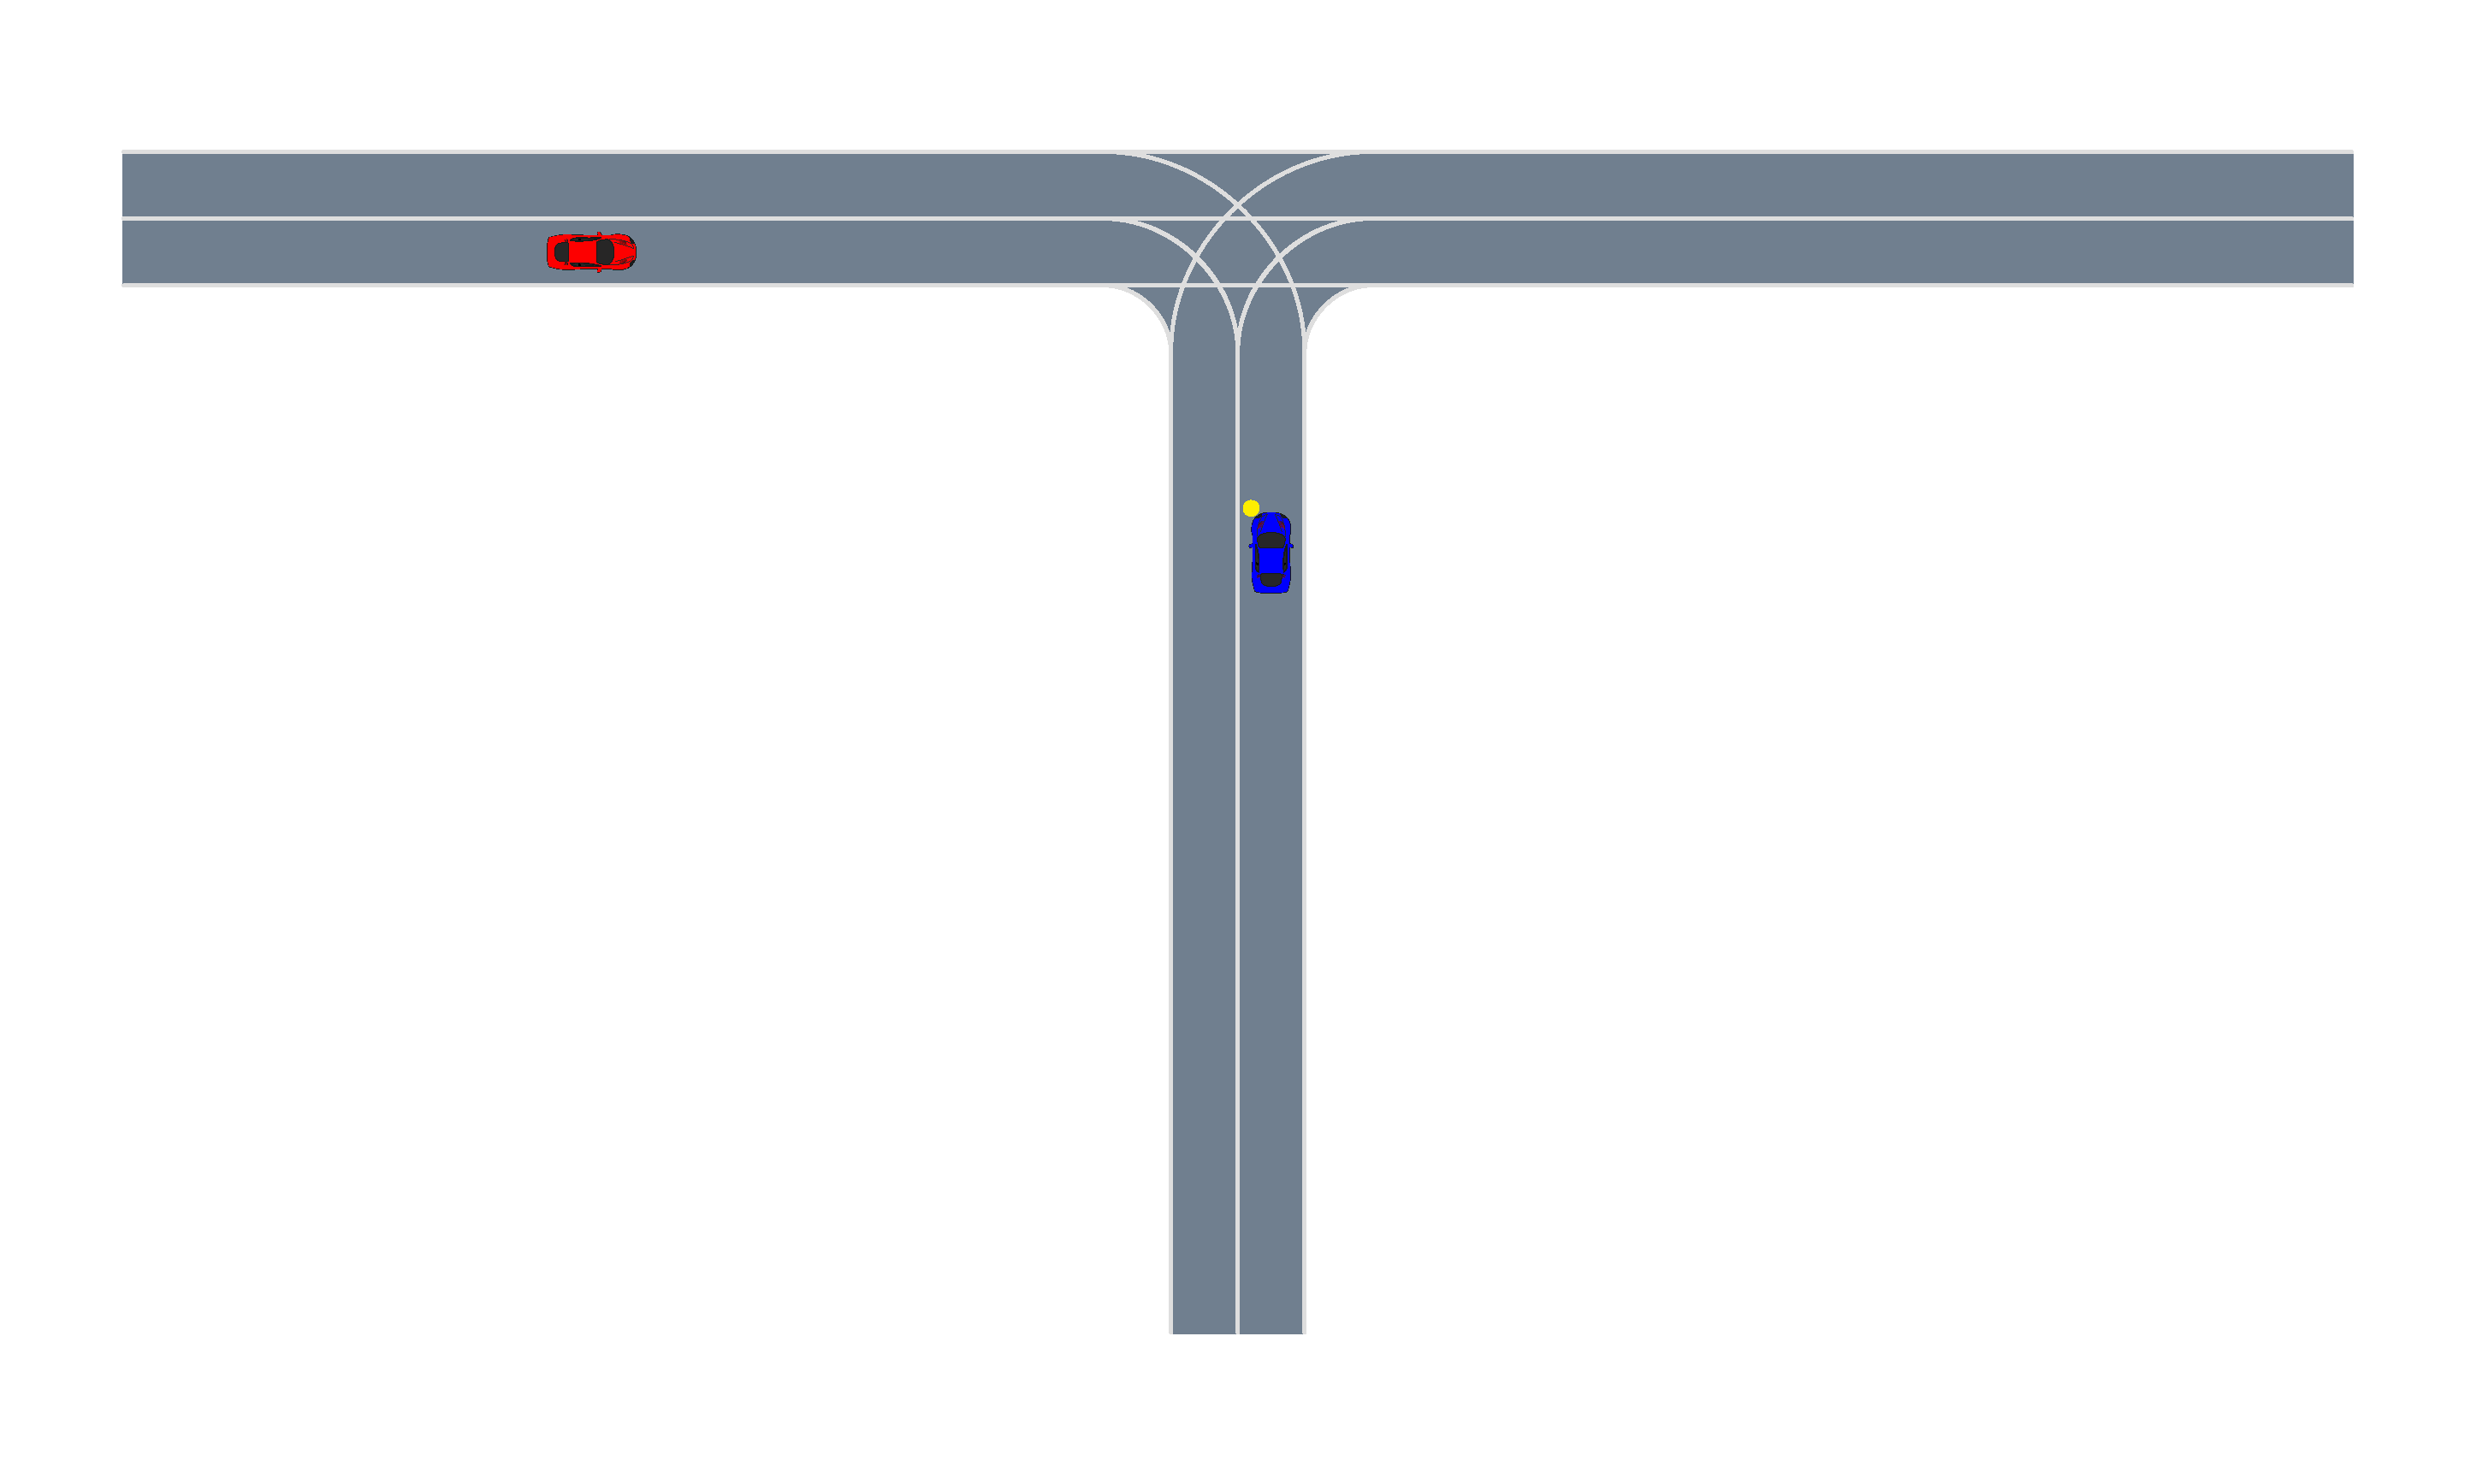
\includegraphics[width=0.9\textwidth, trim={10cm 16.5cm 22cm 0},clip]{figures/interpretable_validation/2car_res1_frame_01.pdf}
    \end{subfigure}%
   \begin{subfigure}[t]{0.33\columnwidth}
        \centering
        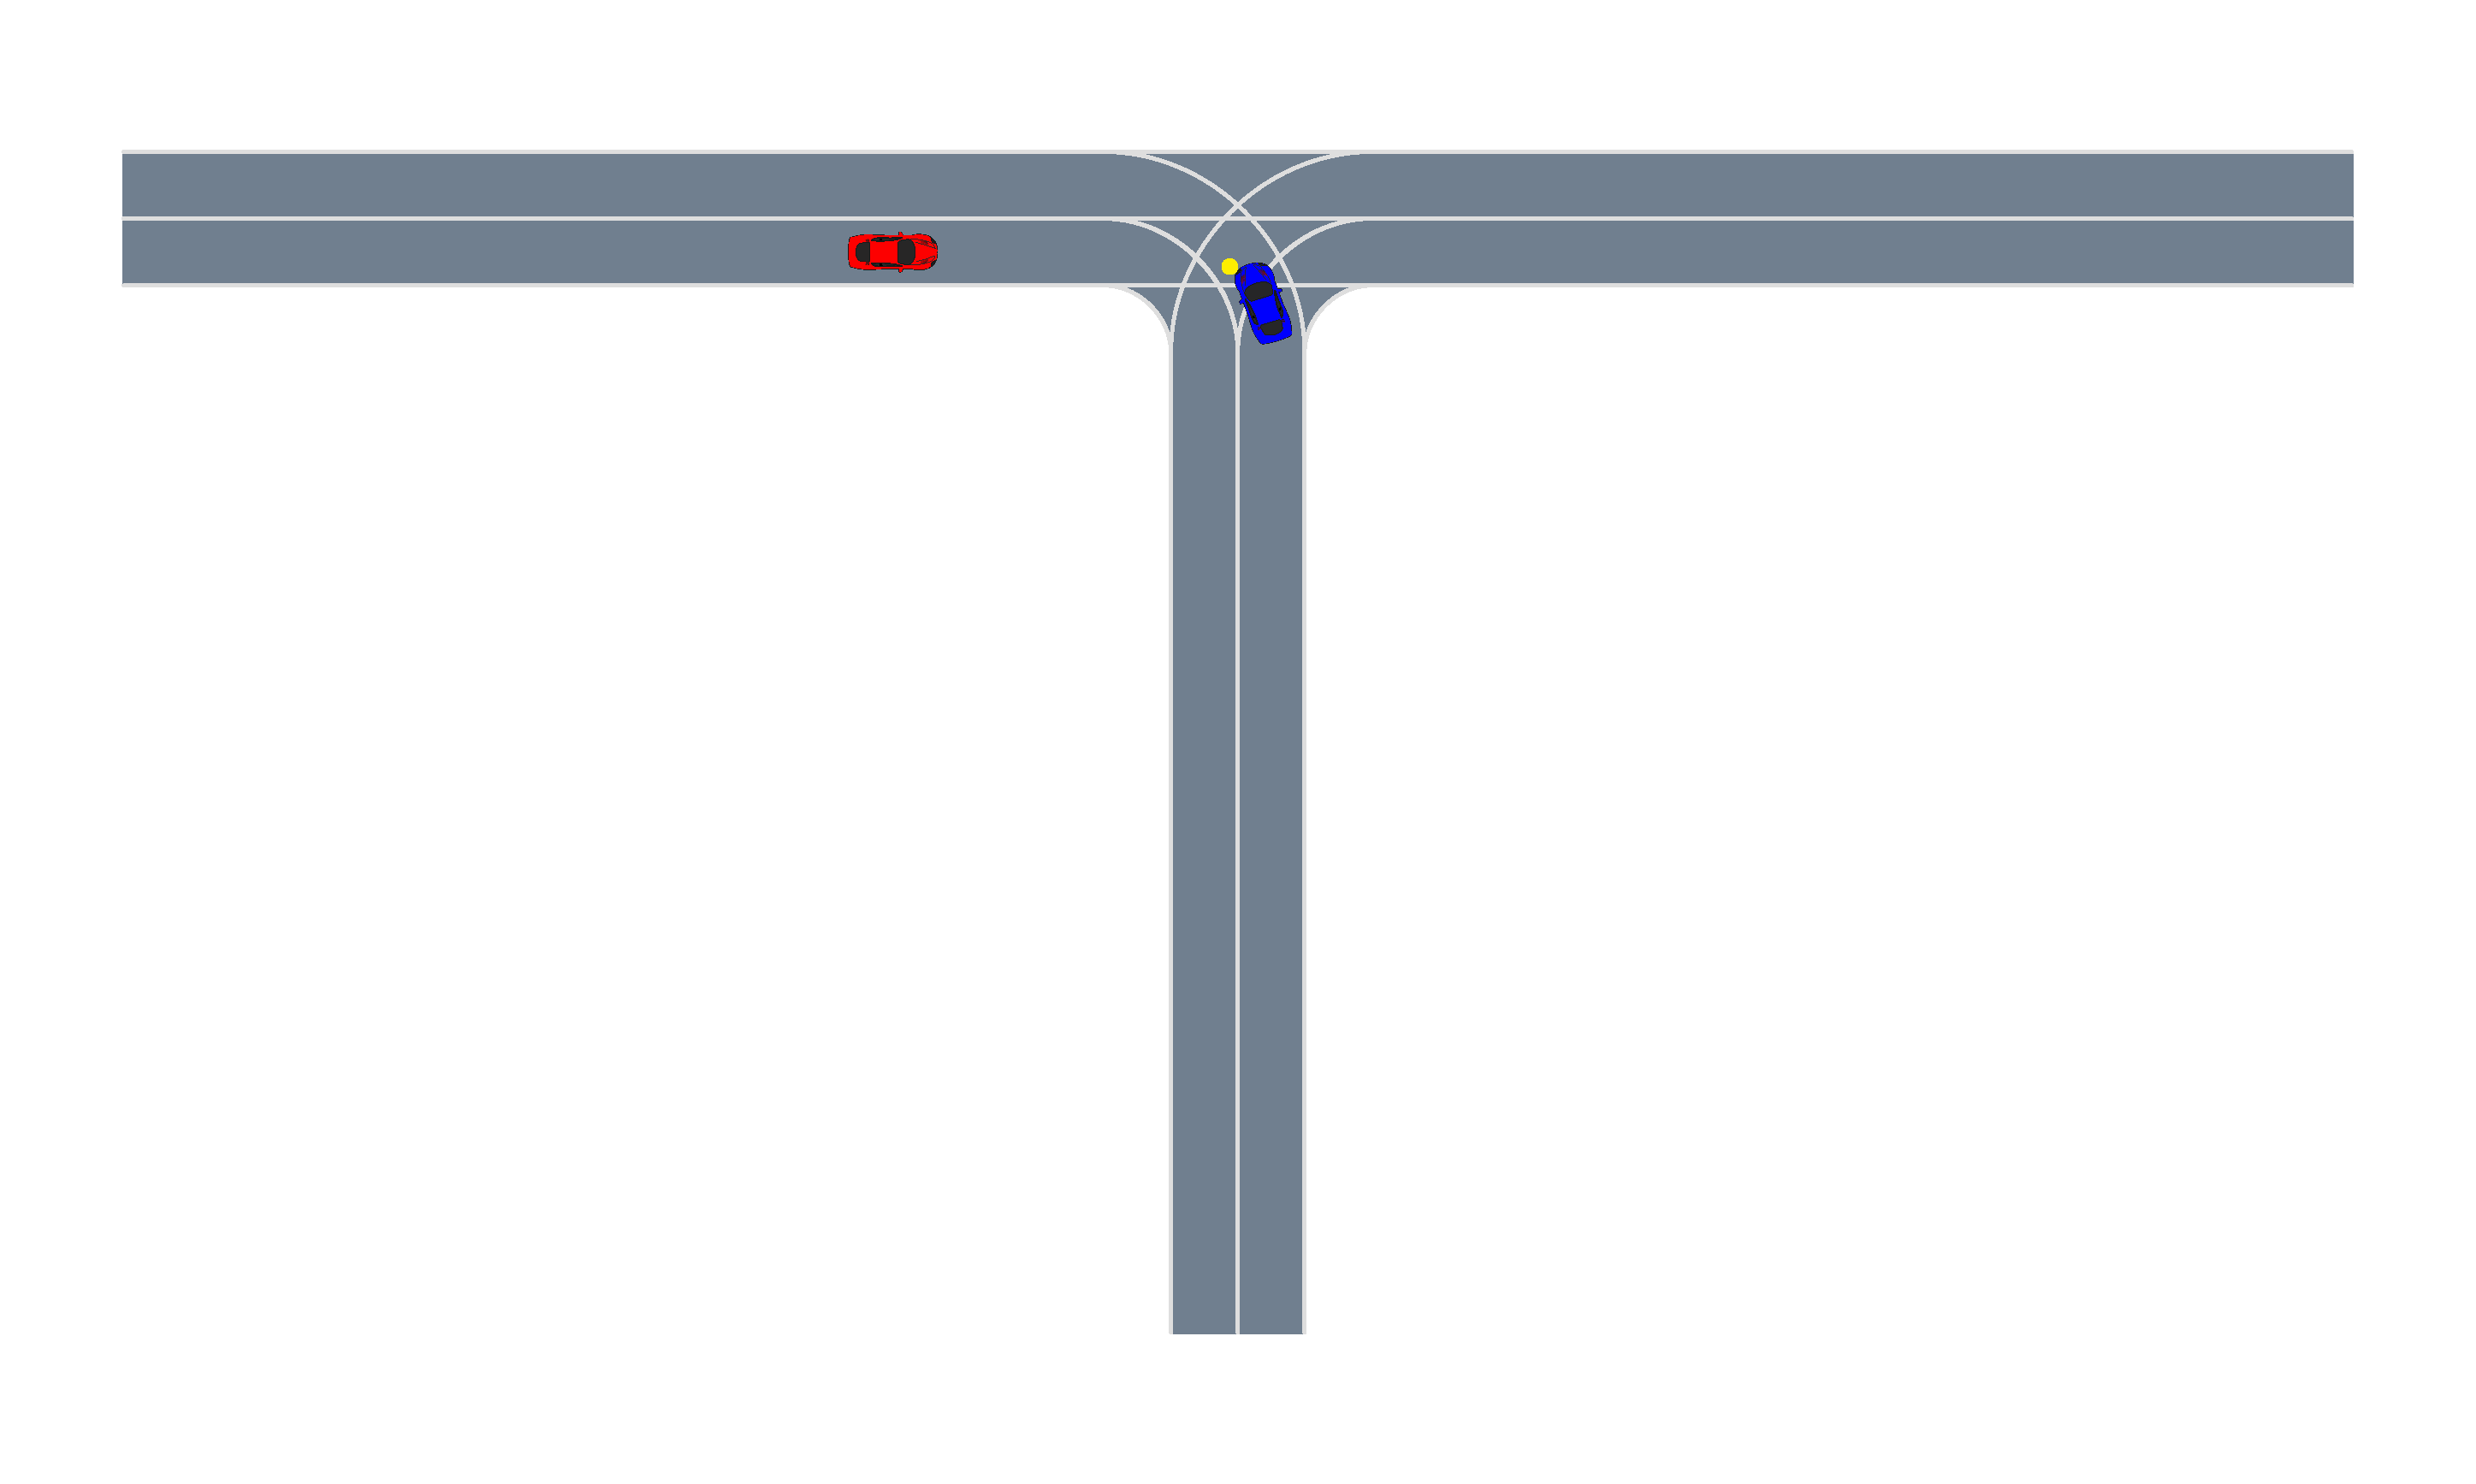
\includegraphics[width=0.9\textwidth, trim={10cm 16.5cm 22cm 0},clip]{figures/interpretable_validation/2car_res1_frame_07.pdf}
    \end{subfigure}%
    \begin{subfigure}[t]{0.33\columnwidth}
        \centering
        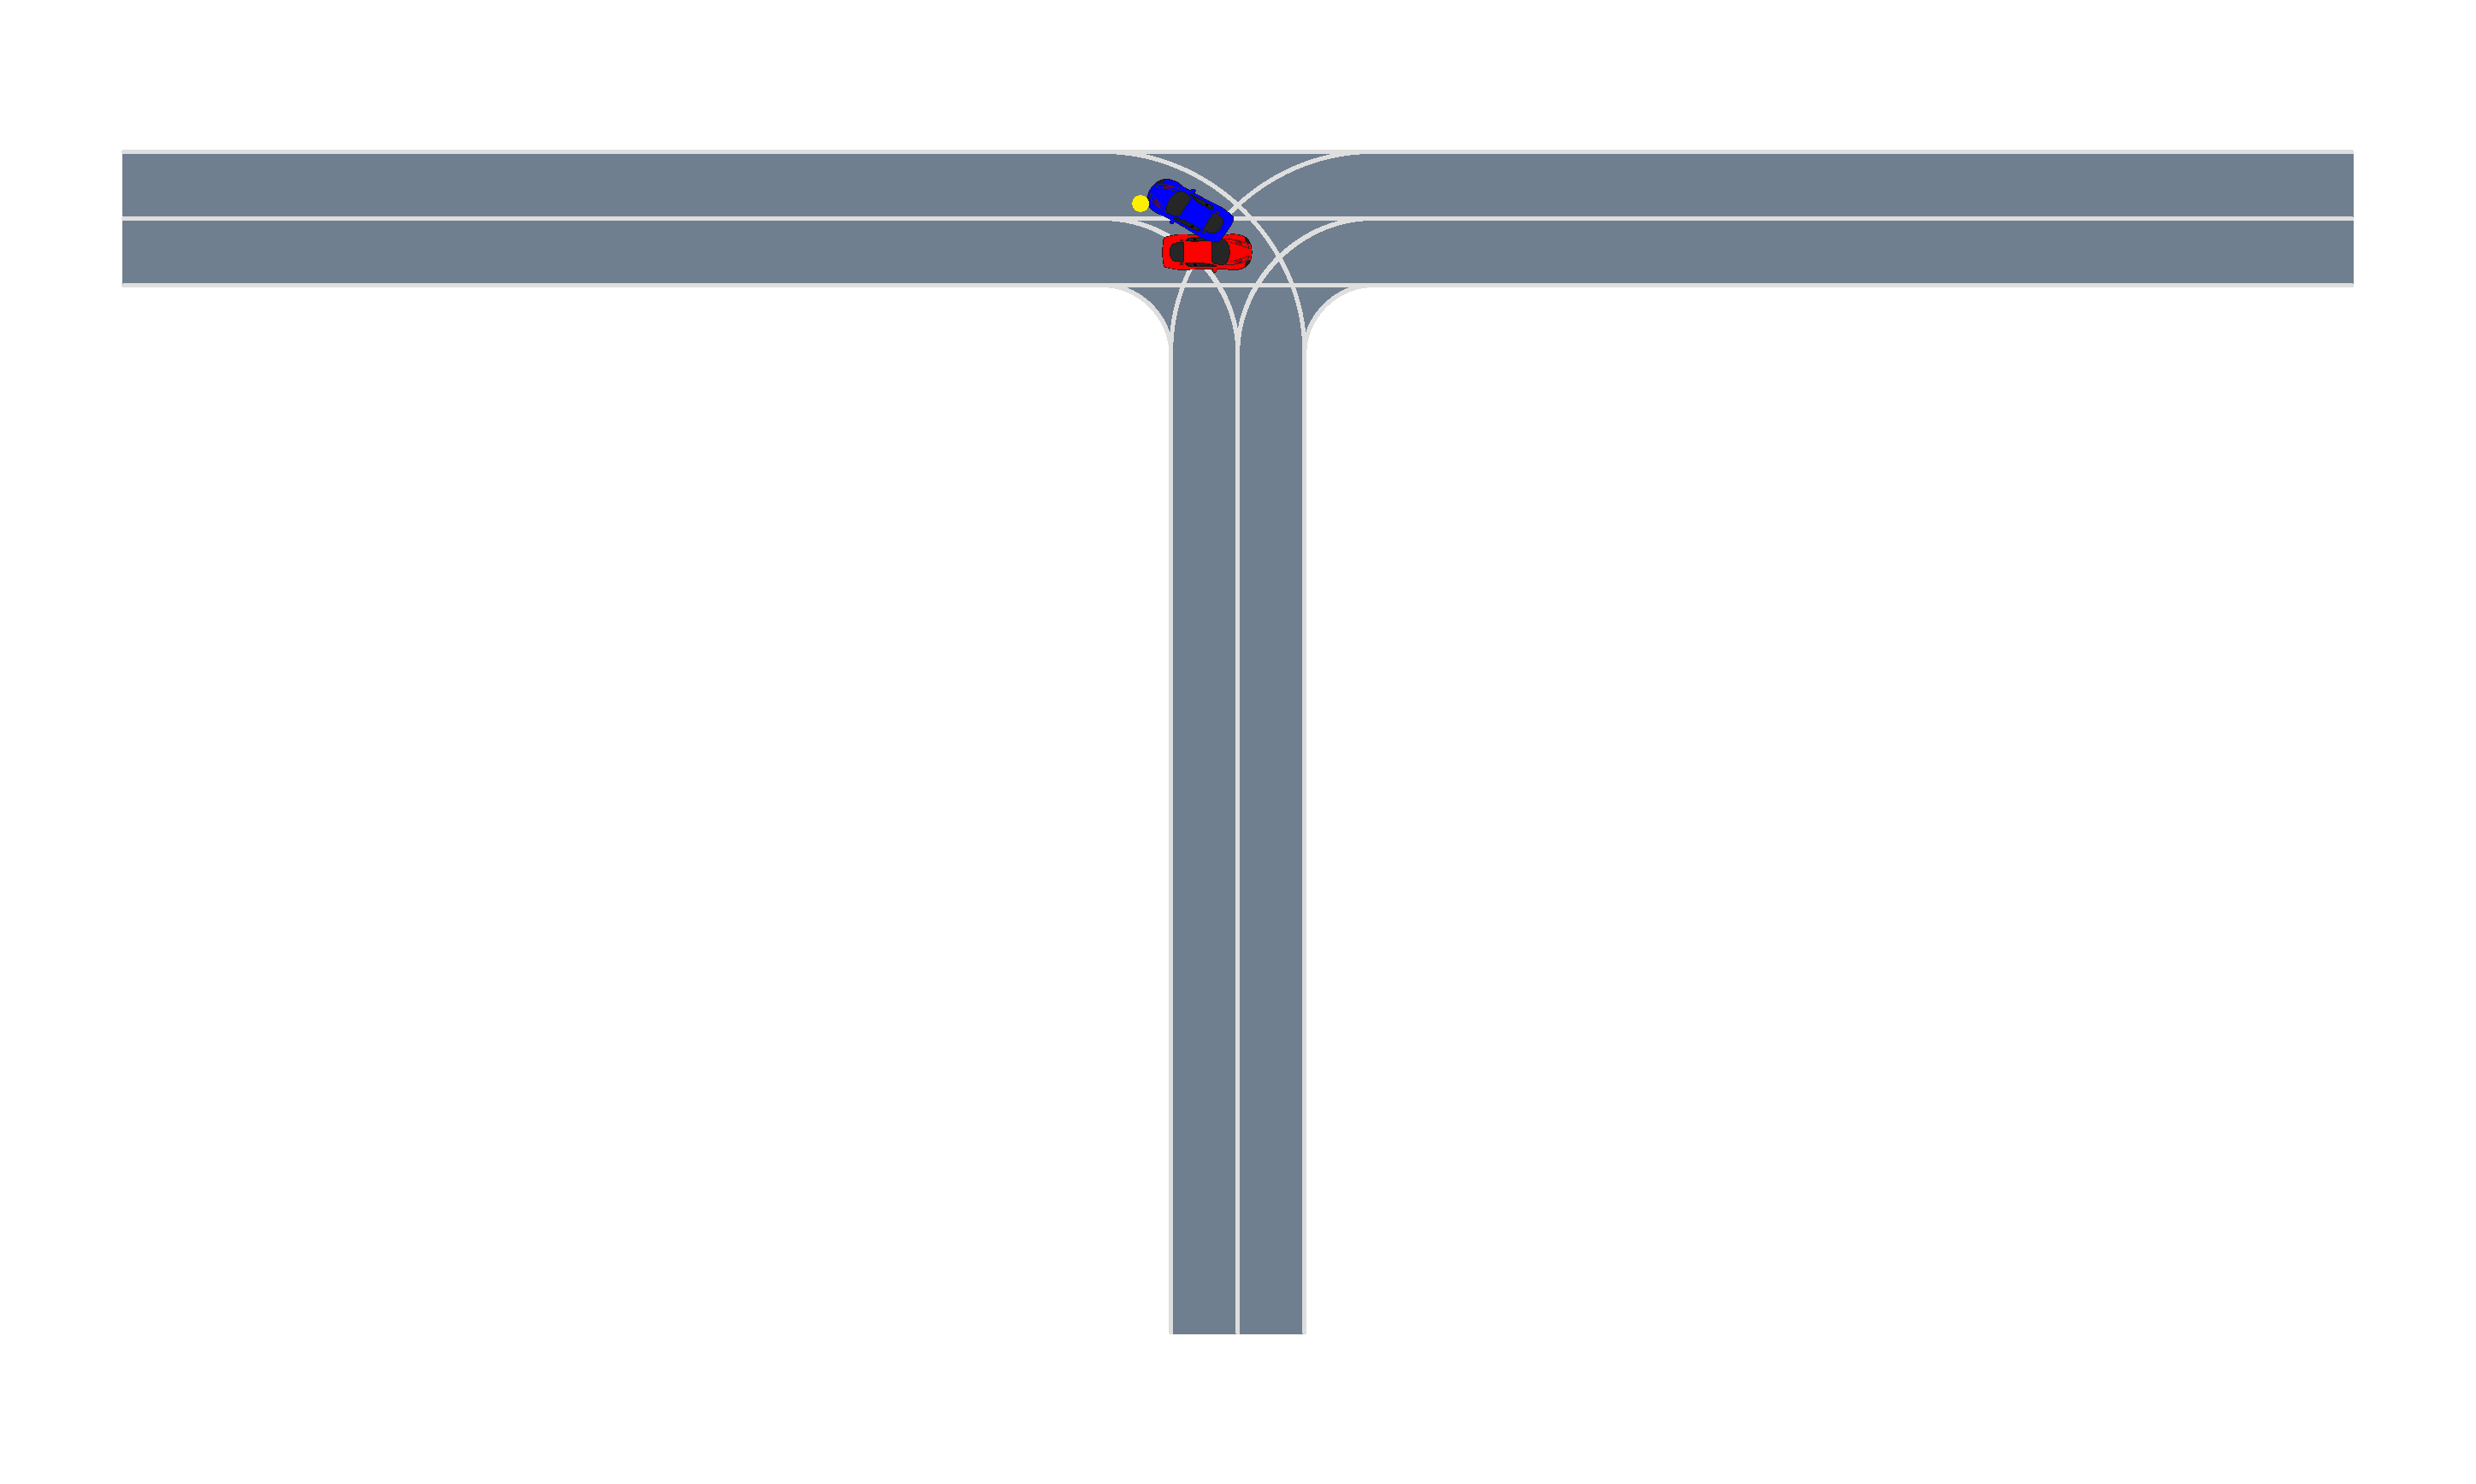
\includegraphics[width=0.9\textwidth, trim={10cm 16.5cm 22cm 0},clip]{figures/interpretable_validation/2car_res1_frame_12.pdf}
    \end{subfigure}
    \caption{Collision for LT1 at $t=(\SI{0}{s}, \SI{1.08}{s}, \SI{1.98}{s})$.}
    \label{fig:2car_LT1}
\end{figure}


%%%% Second initial condition
\begin{figure}
    \centering
    \begin{subfigure}[t]{0.33\columnwidth}
        \centering
        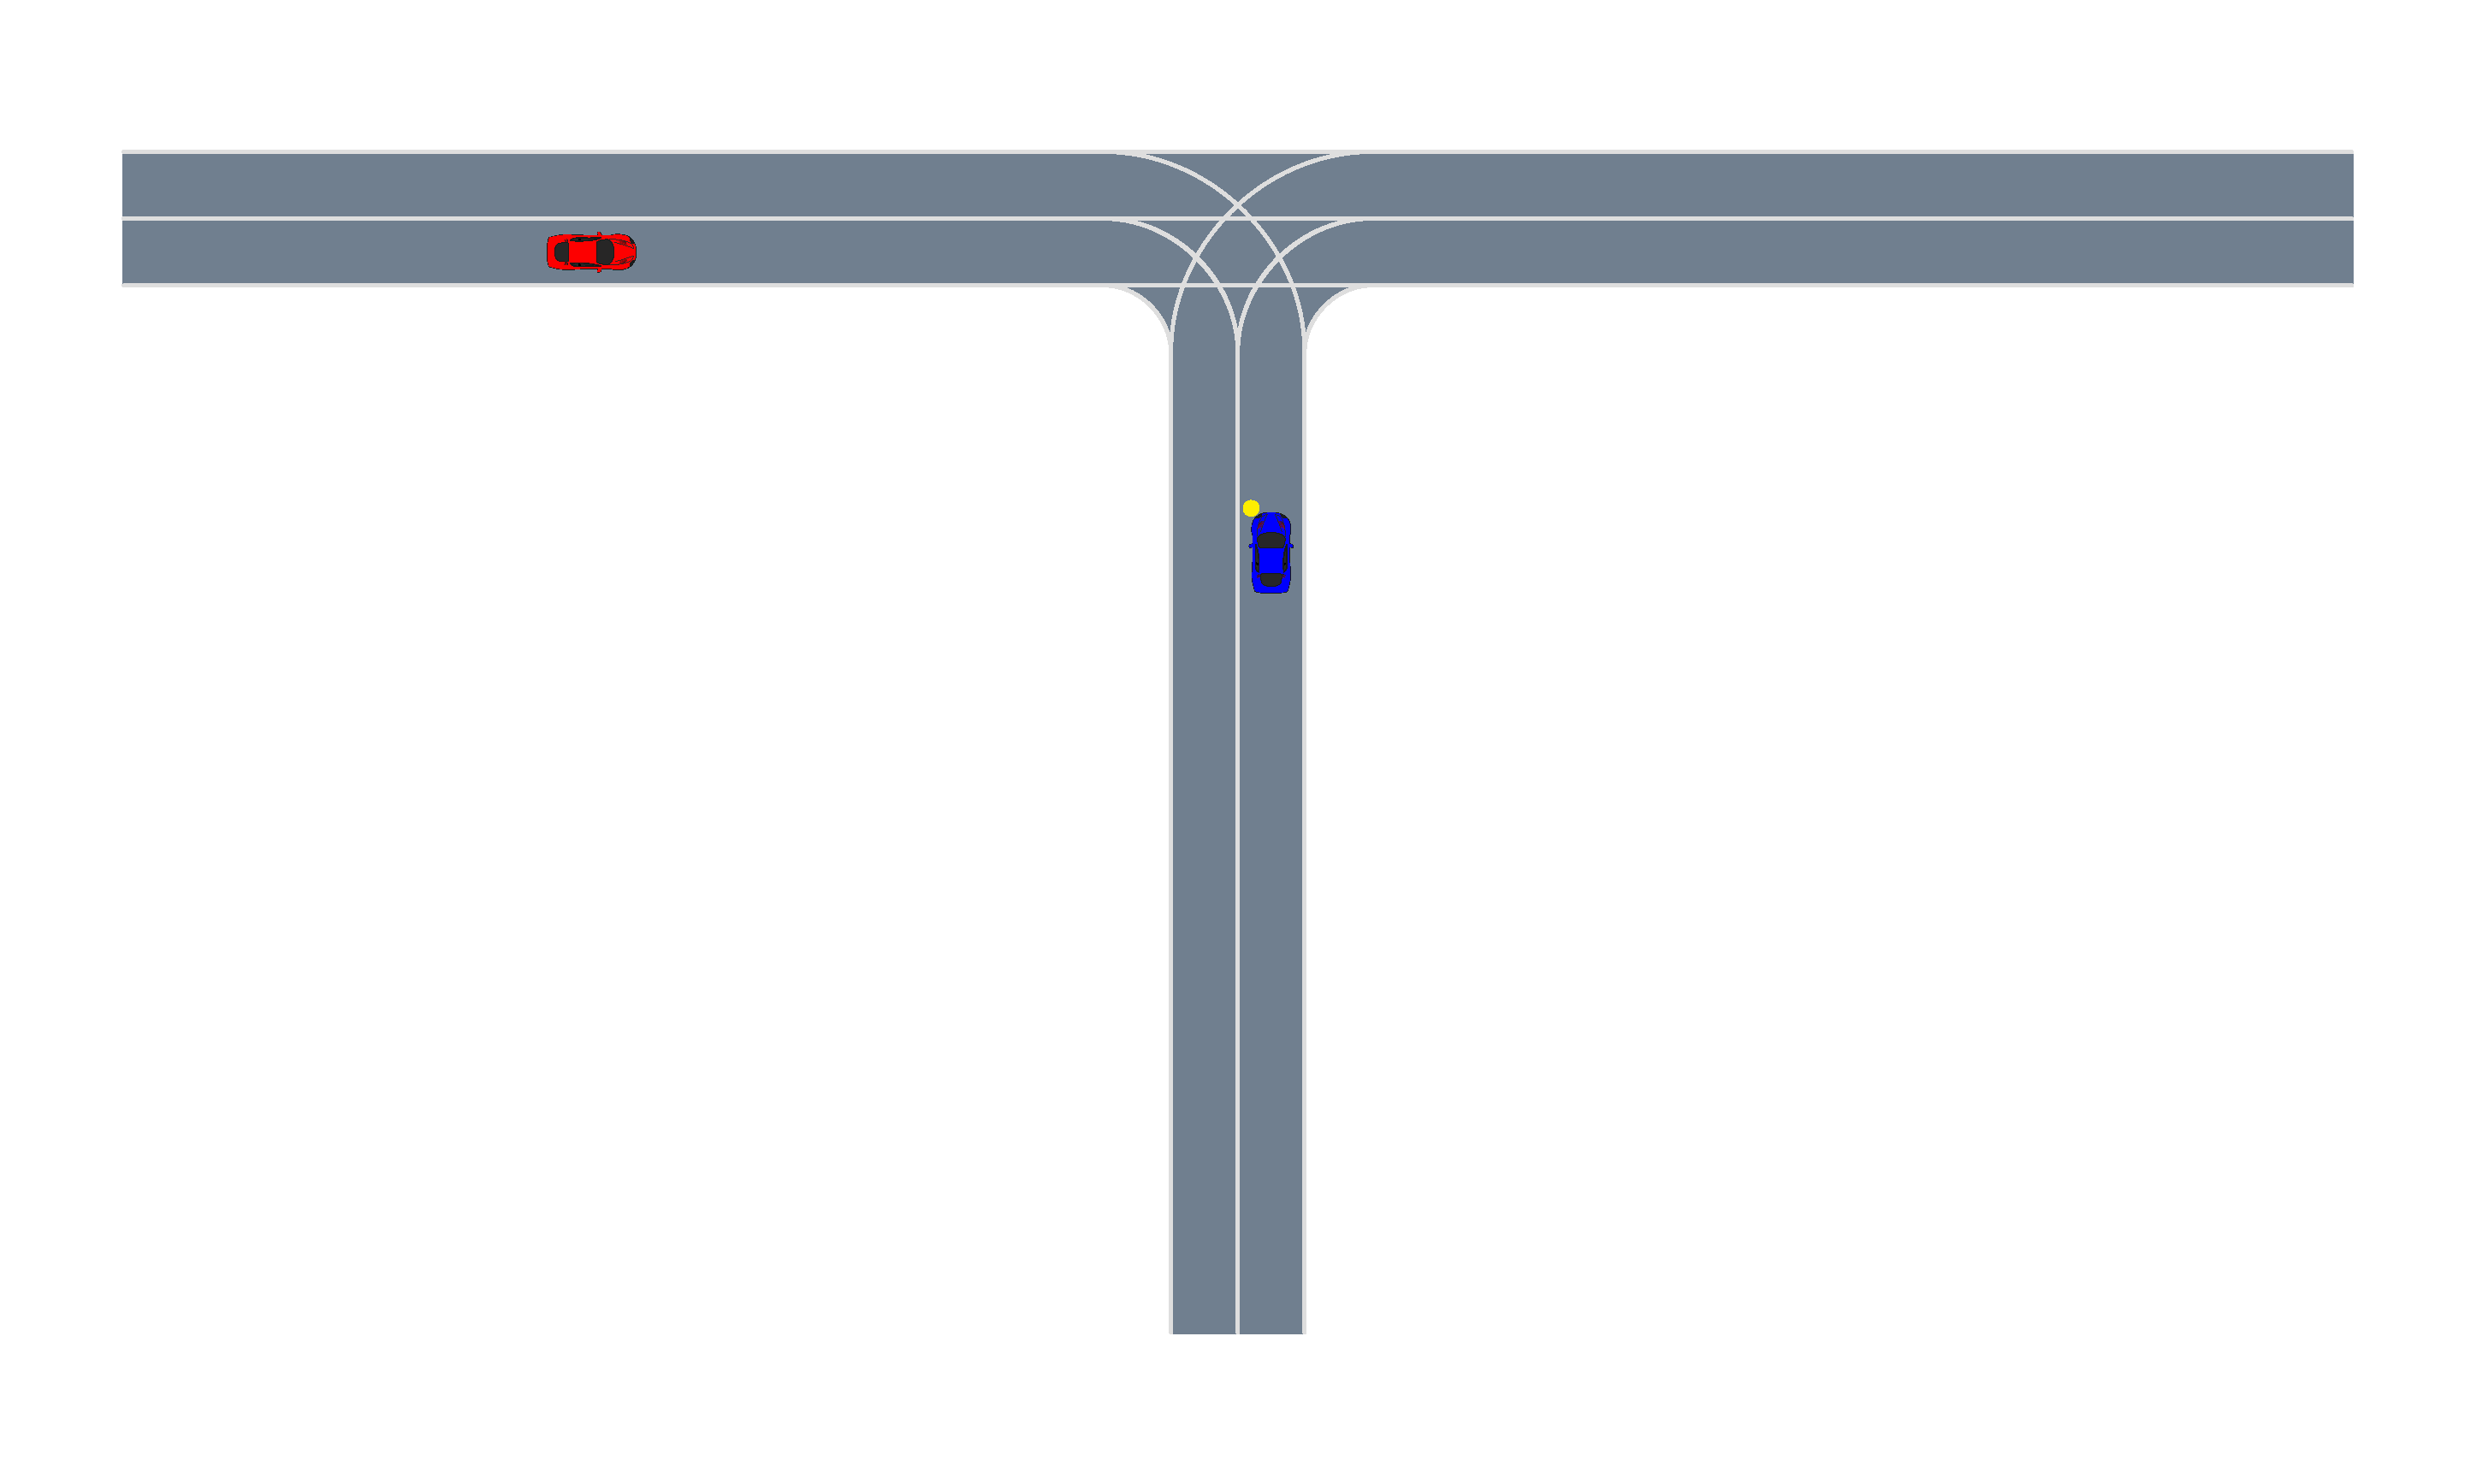
\includegraphics[width=0.9\textwidth, trim={10cm 16.5cm 22cm 0},clip]{figures/interpretable_validation/2car_res2_frame_01.pdf}
    \end{subfigure}%
   \begin{subfigure}[t]{0.33\columnwidth}
        \centering
        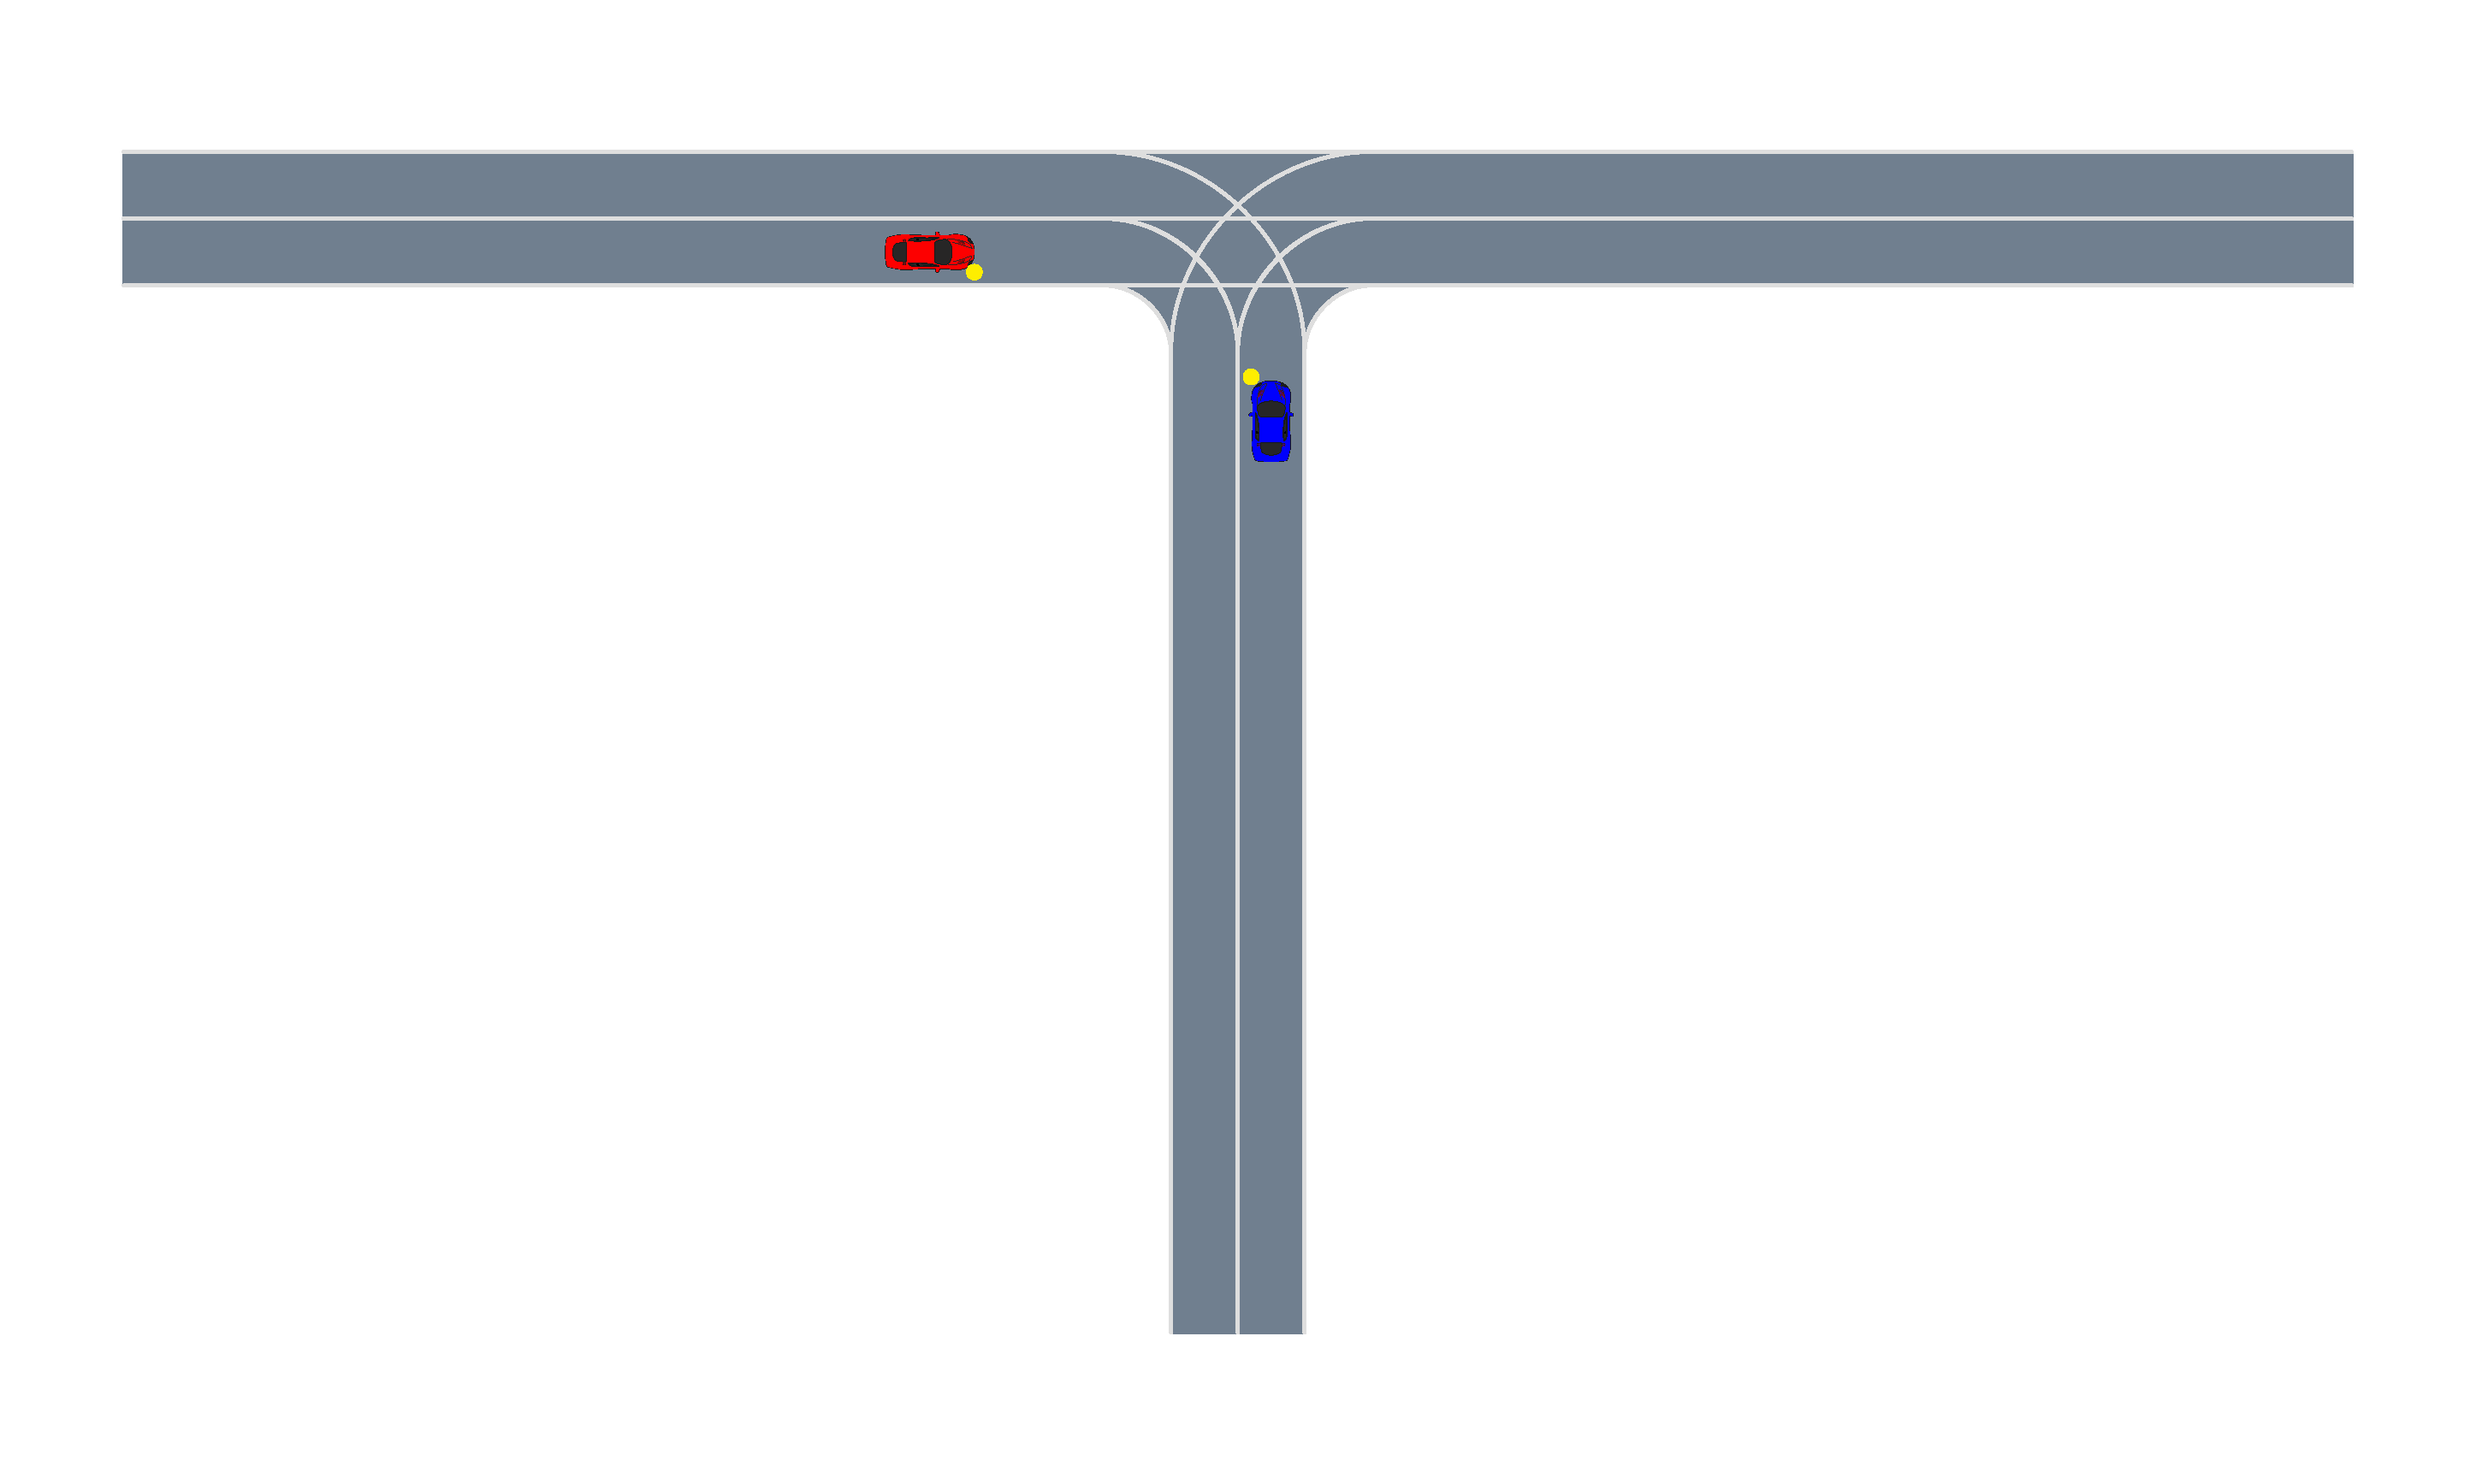
\includegraphics[width=0.9\textwidth, trim={10cm 16.5cm 22cm 0},clip]{figures/interpretable_validation/2car_res2_frame_05.pdf}
    \end{subfigure}%
    \begin{subfigure}[t]{0.33\columnwidth}
        \centering
        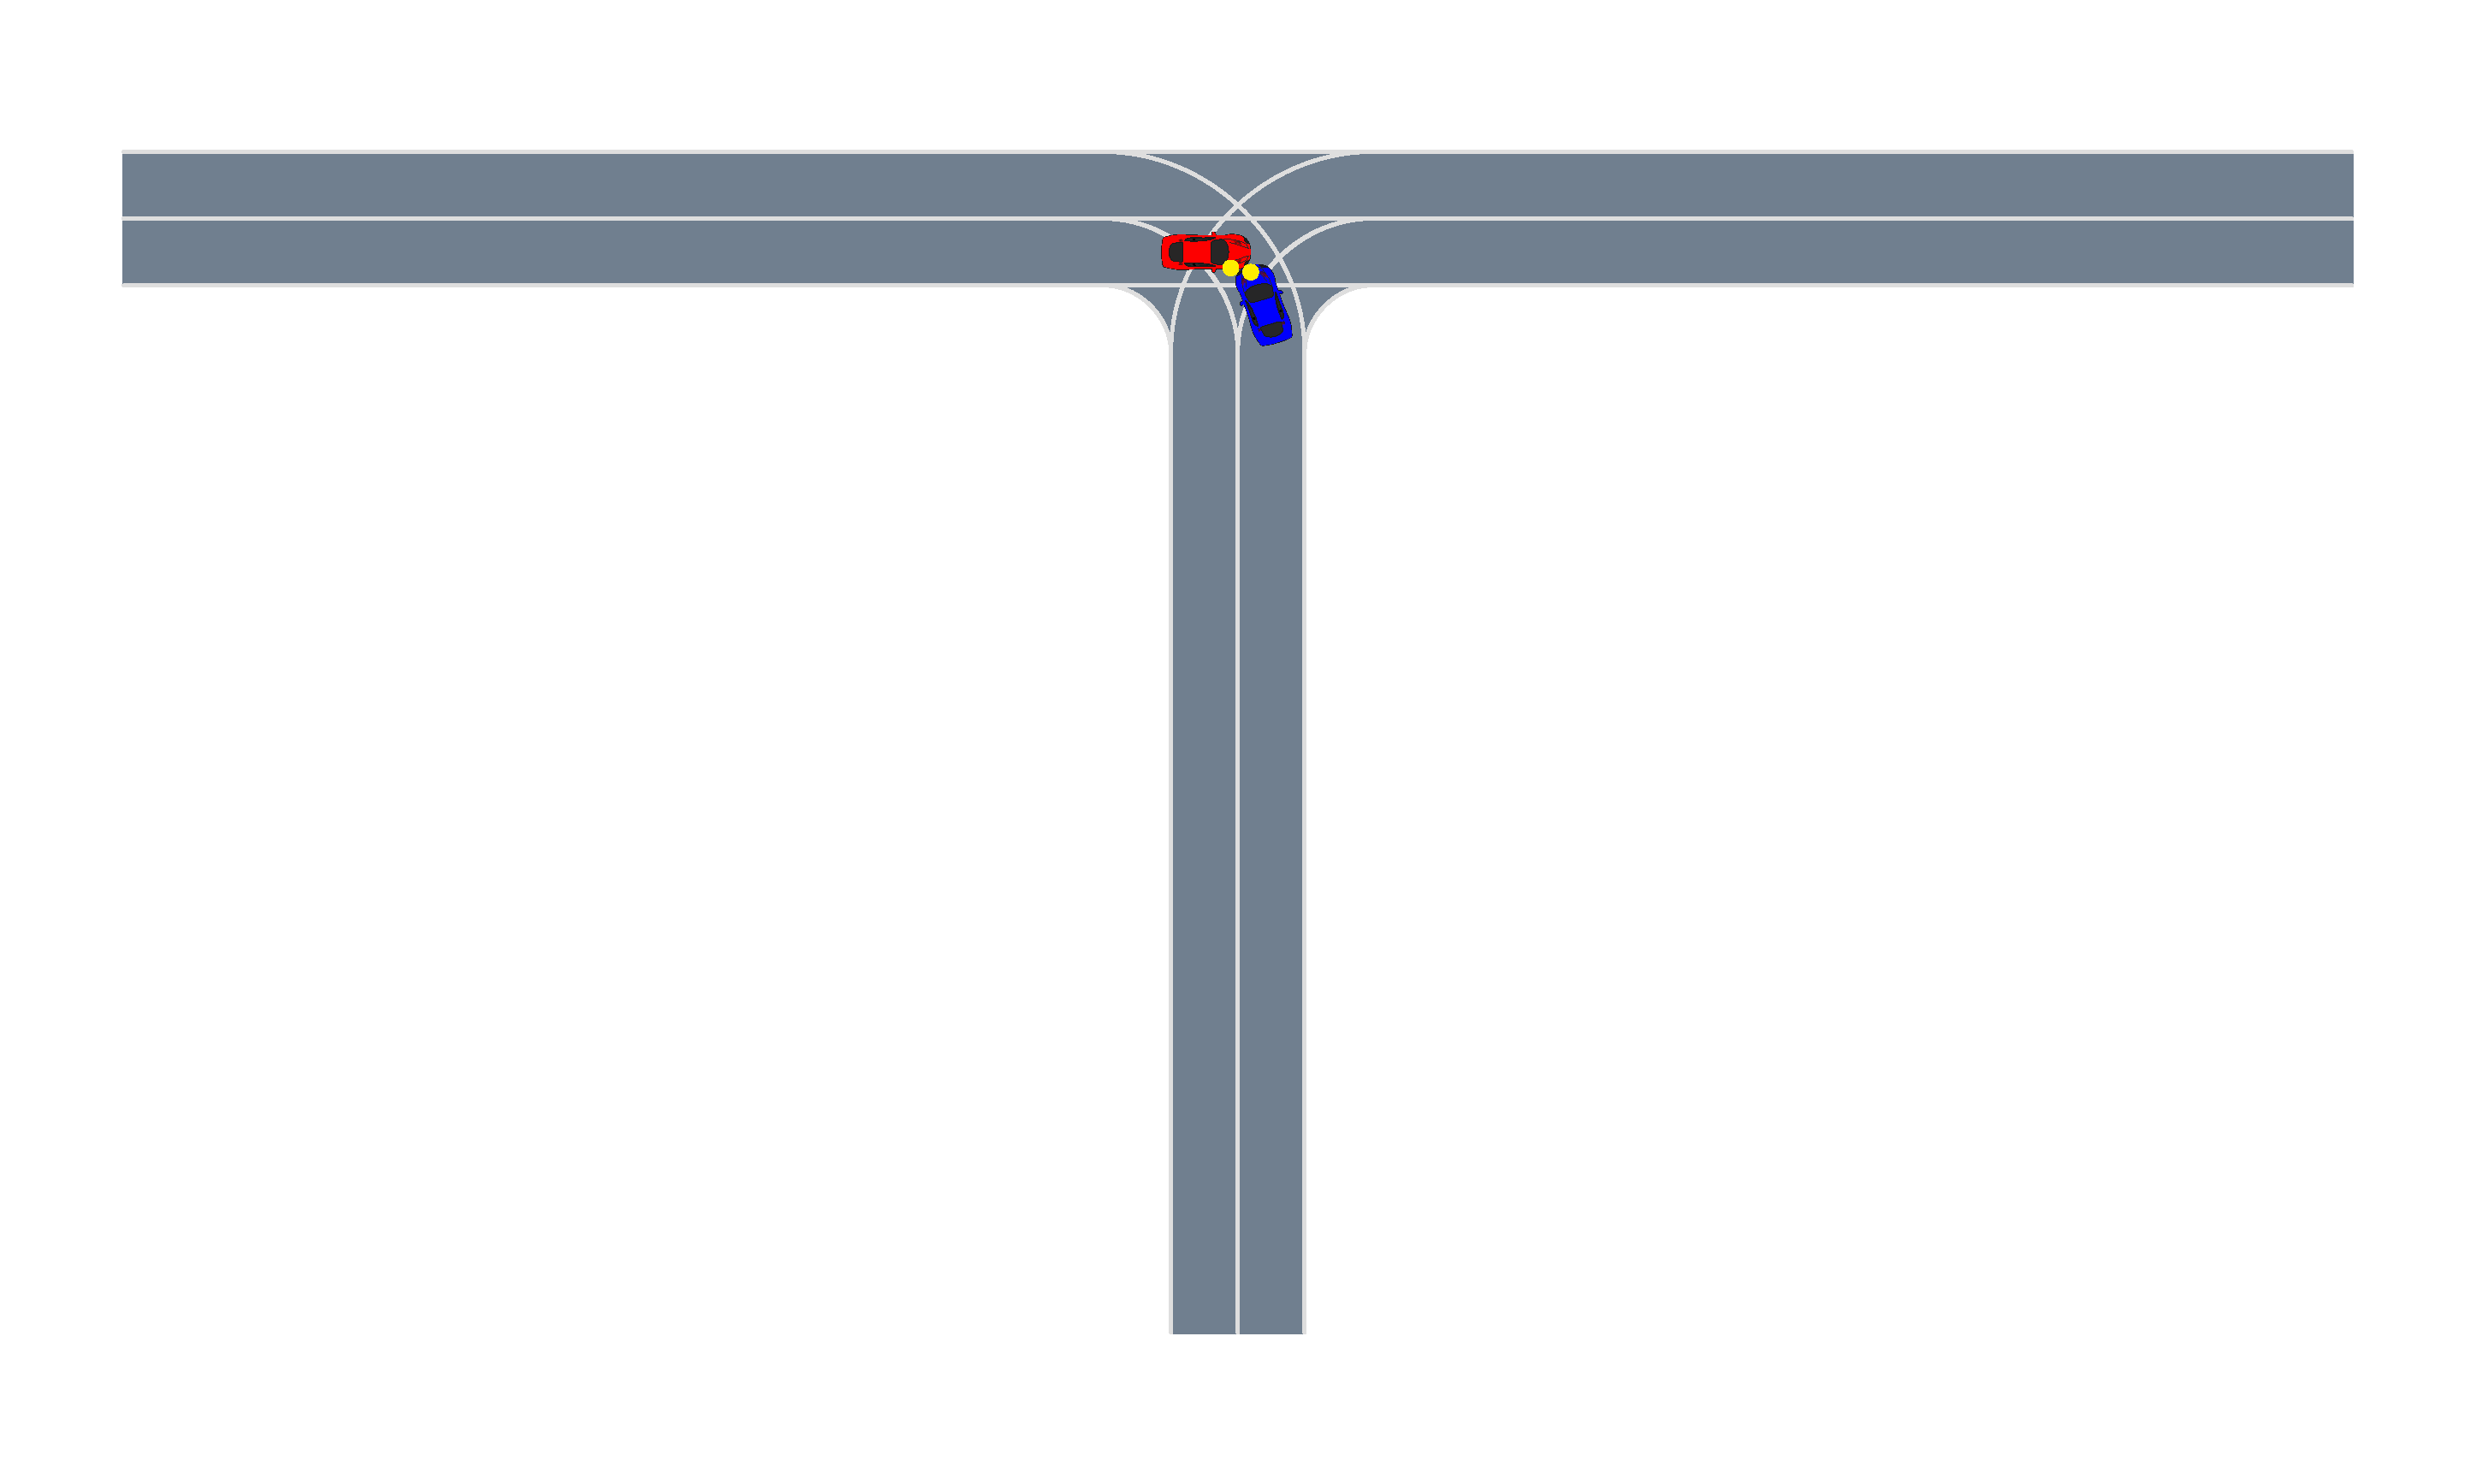
\includegraphics[width=0.9\textwidth, trim={10cm 16.5cm 22cm 0},clip]{figures/interpretable_validation/2car_res2_frame_08.pdf}
    \end{subfigure}
    \caption{Collision for LT2 at $t=(\SI{0}{s}, \SI{0.72}{s}, \SI{1.26}{s})$.}
    \label{fig:2car_LT2}
\end{figure}


%%% Third initial condition
\begin{figure}
    \centering
    \begin{subfigure}[t]{0.33\columnwidth}
        \centering
        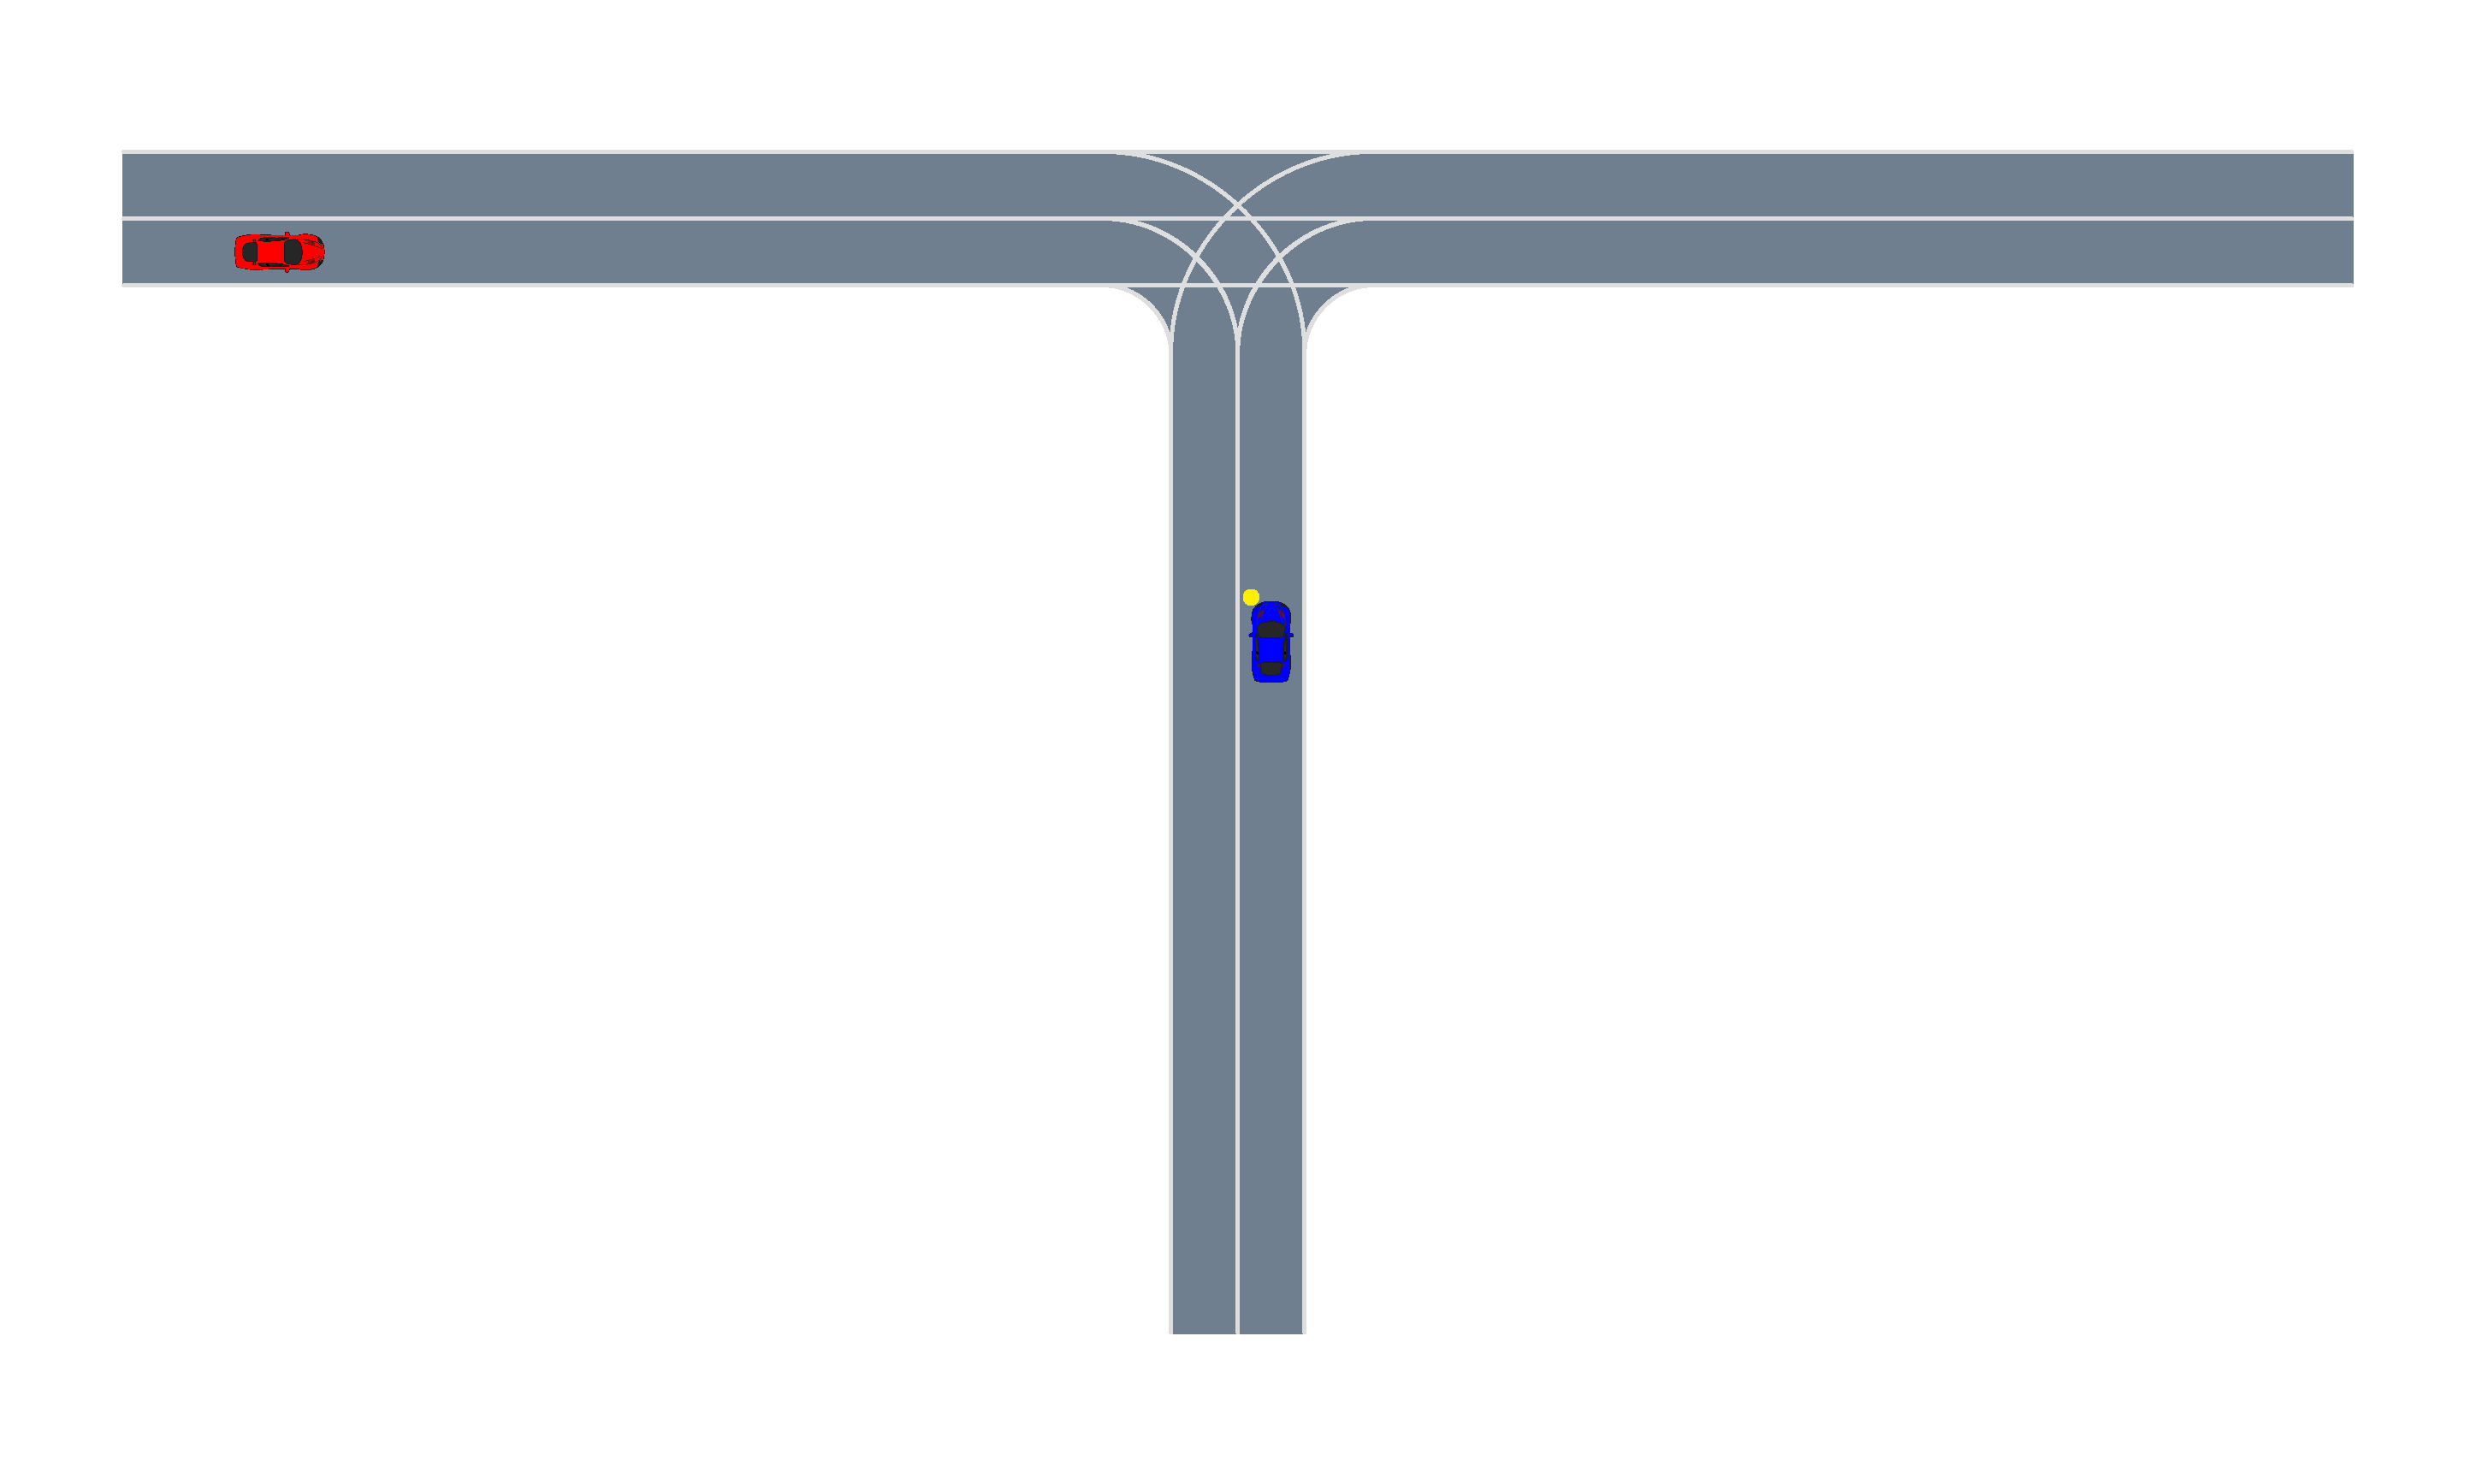
\includegraphics[width=0.9\textwidth, trim={8cm 16cm 22cm 0},clip]{figures/interpretable_validation/2car_res3_frame_01.pdf}
    \end{subfigure}%
   \begin{subfigure}[t]{0.33\columnwidth}
        \centering
        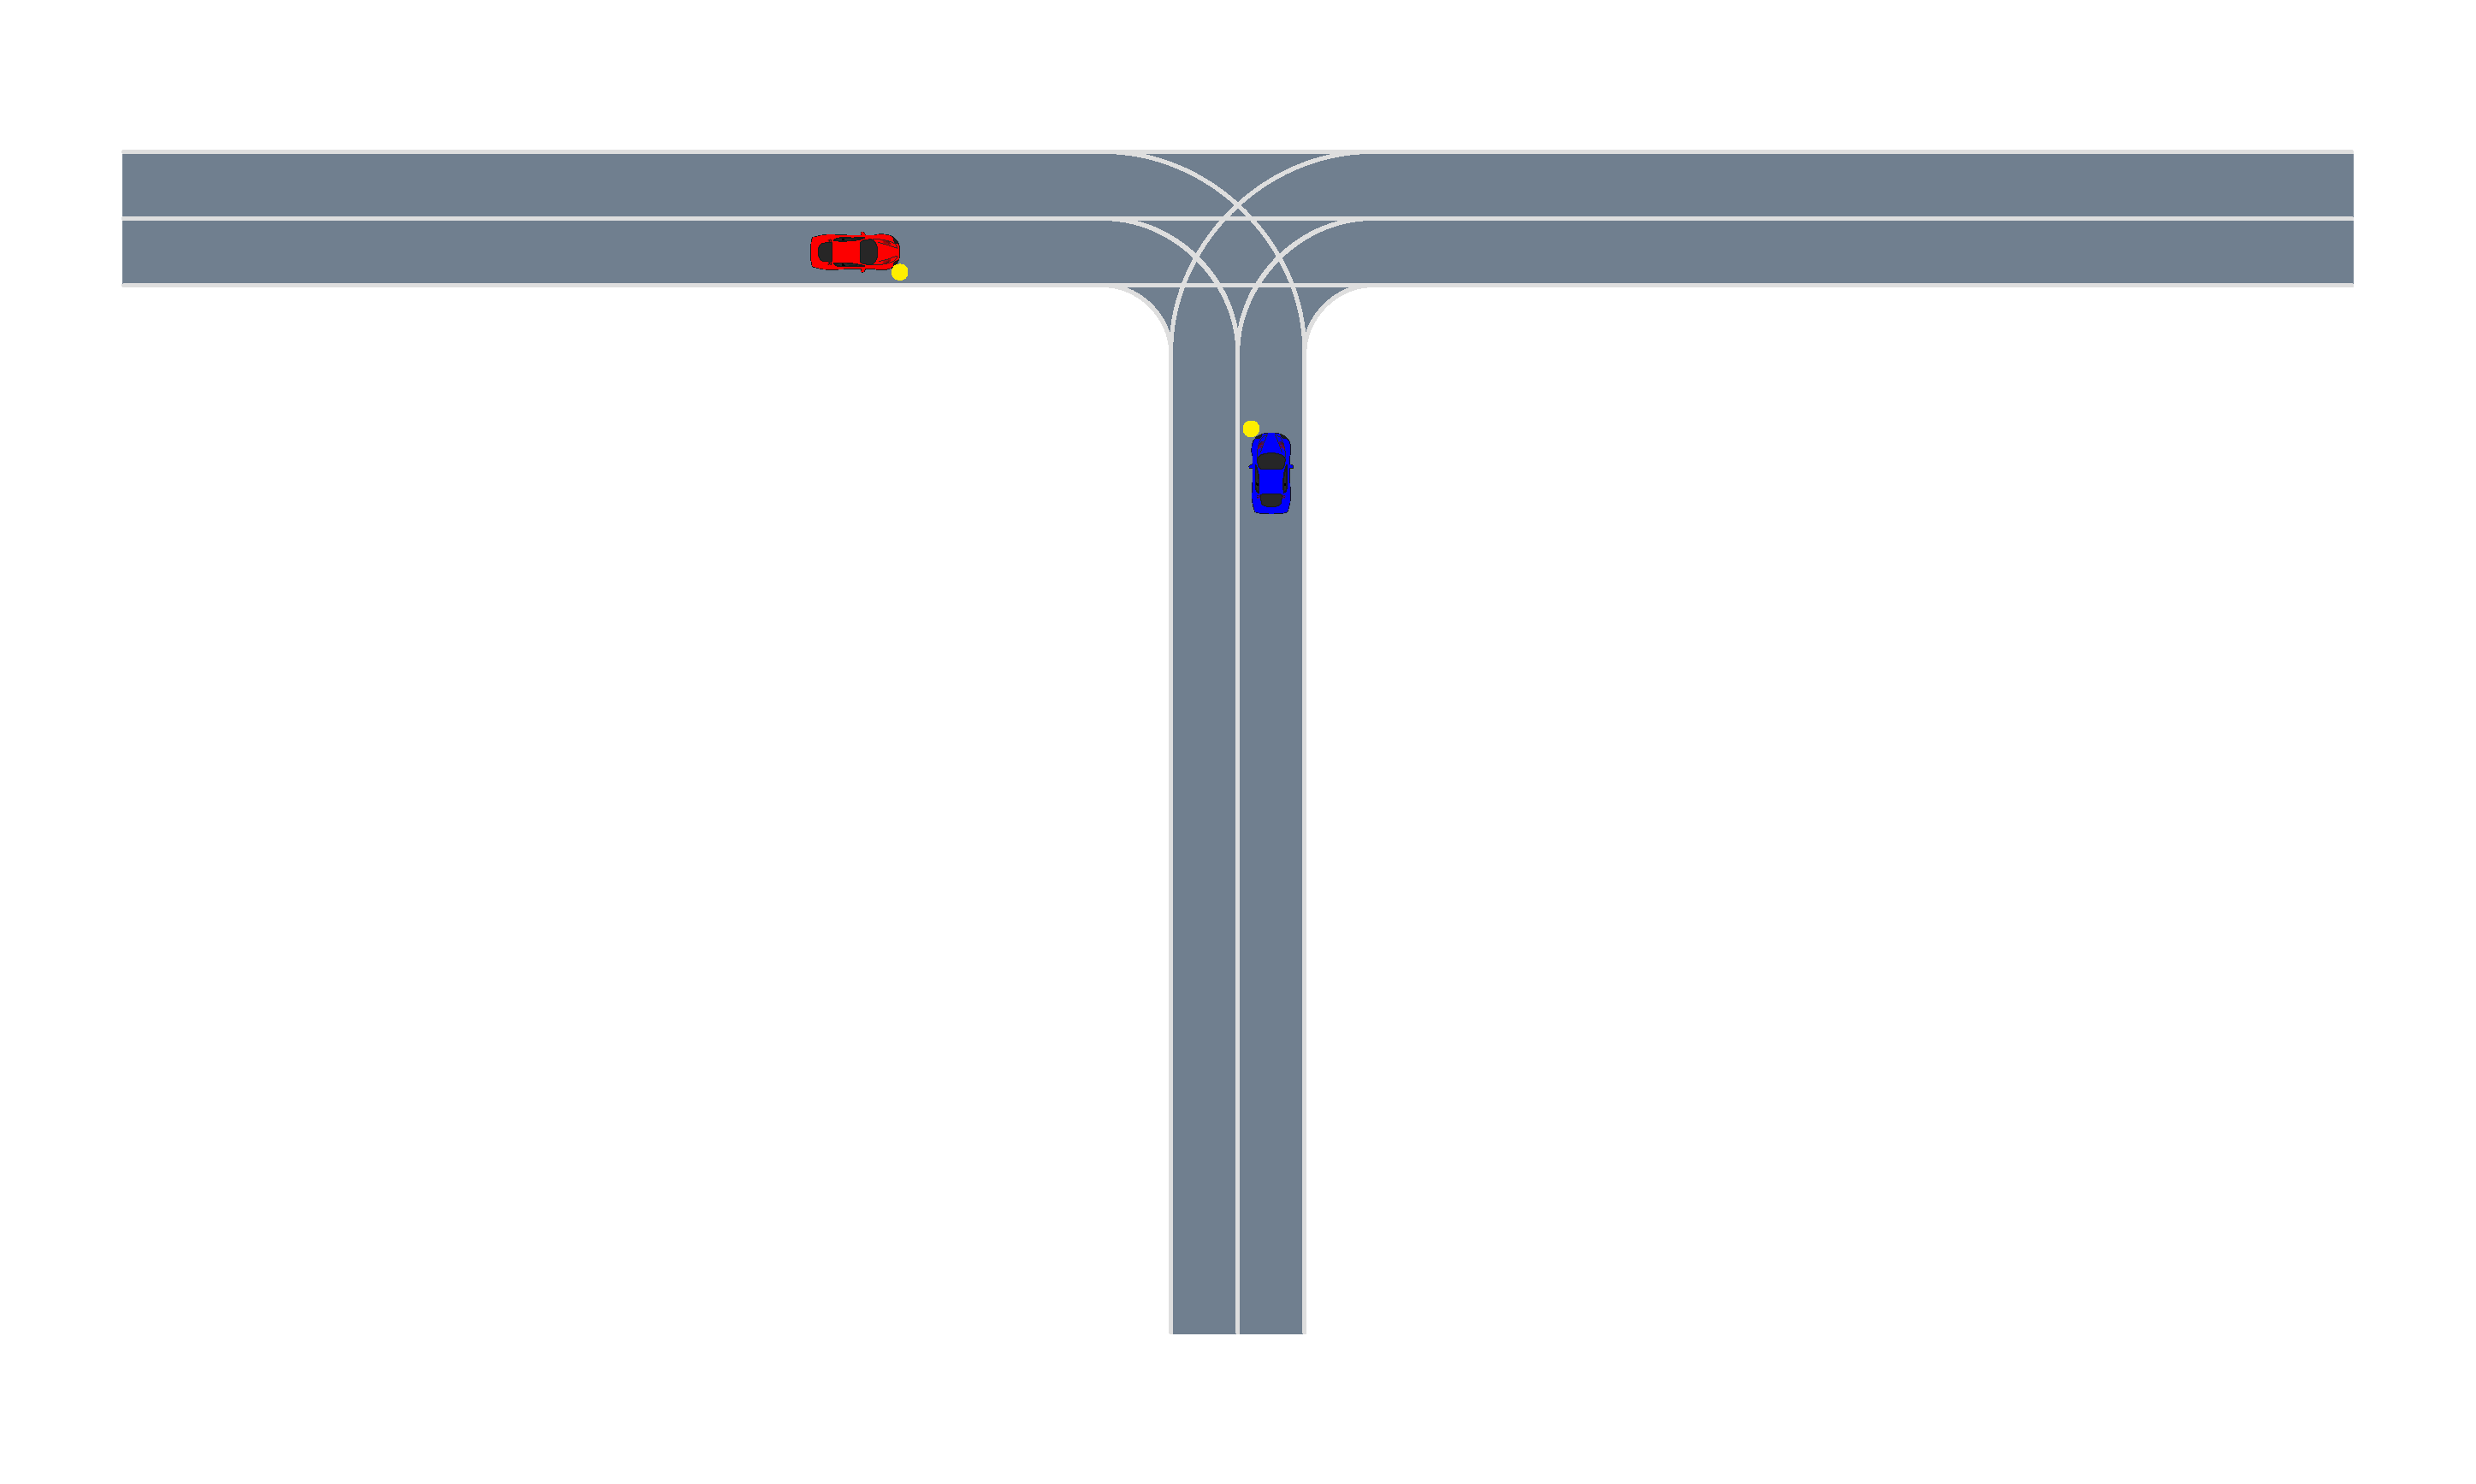
\includegraphics[width=0.9\textwidth, trim={10cm 16.5cm 22cm 0},clip]{figures/interpretable_validation/2car_res3_frame_06.pdf}
    \end{subfigure}%
    \begin{subfigure}[t]{0.33\columnwidth}
        \centering
        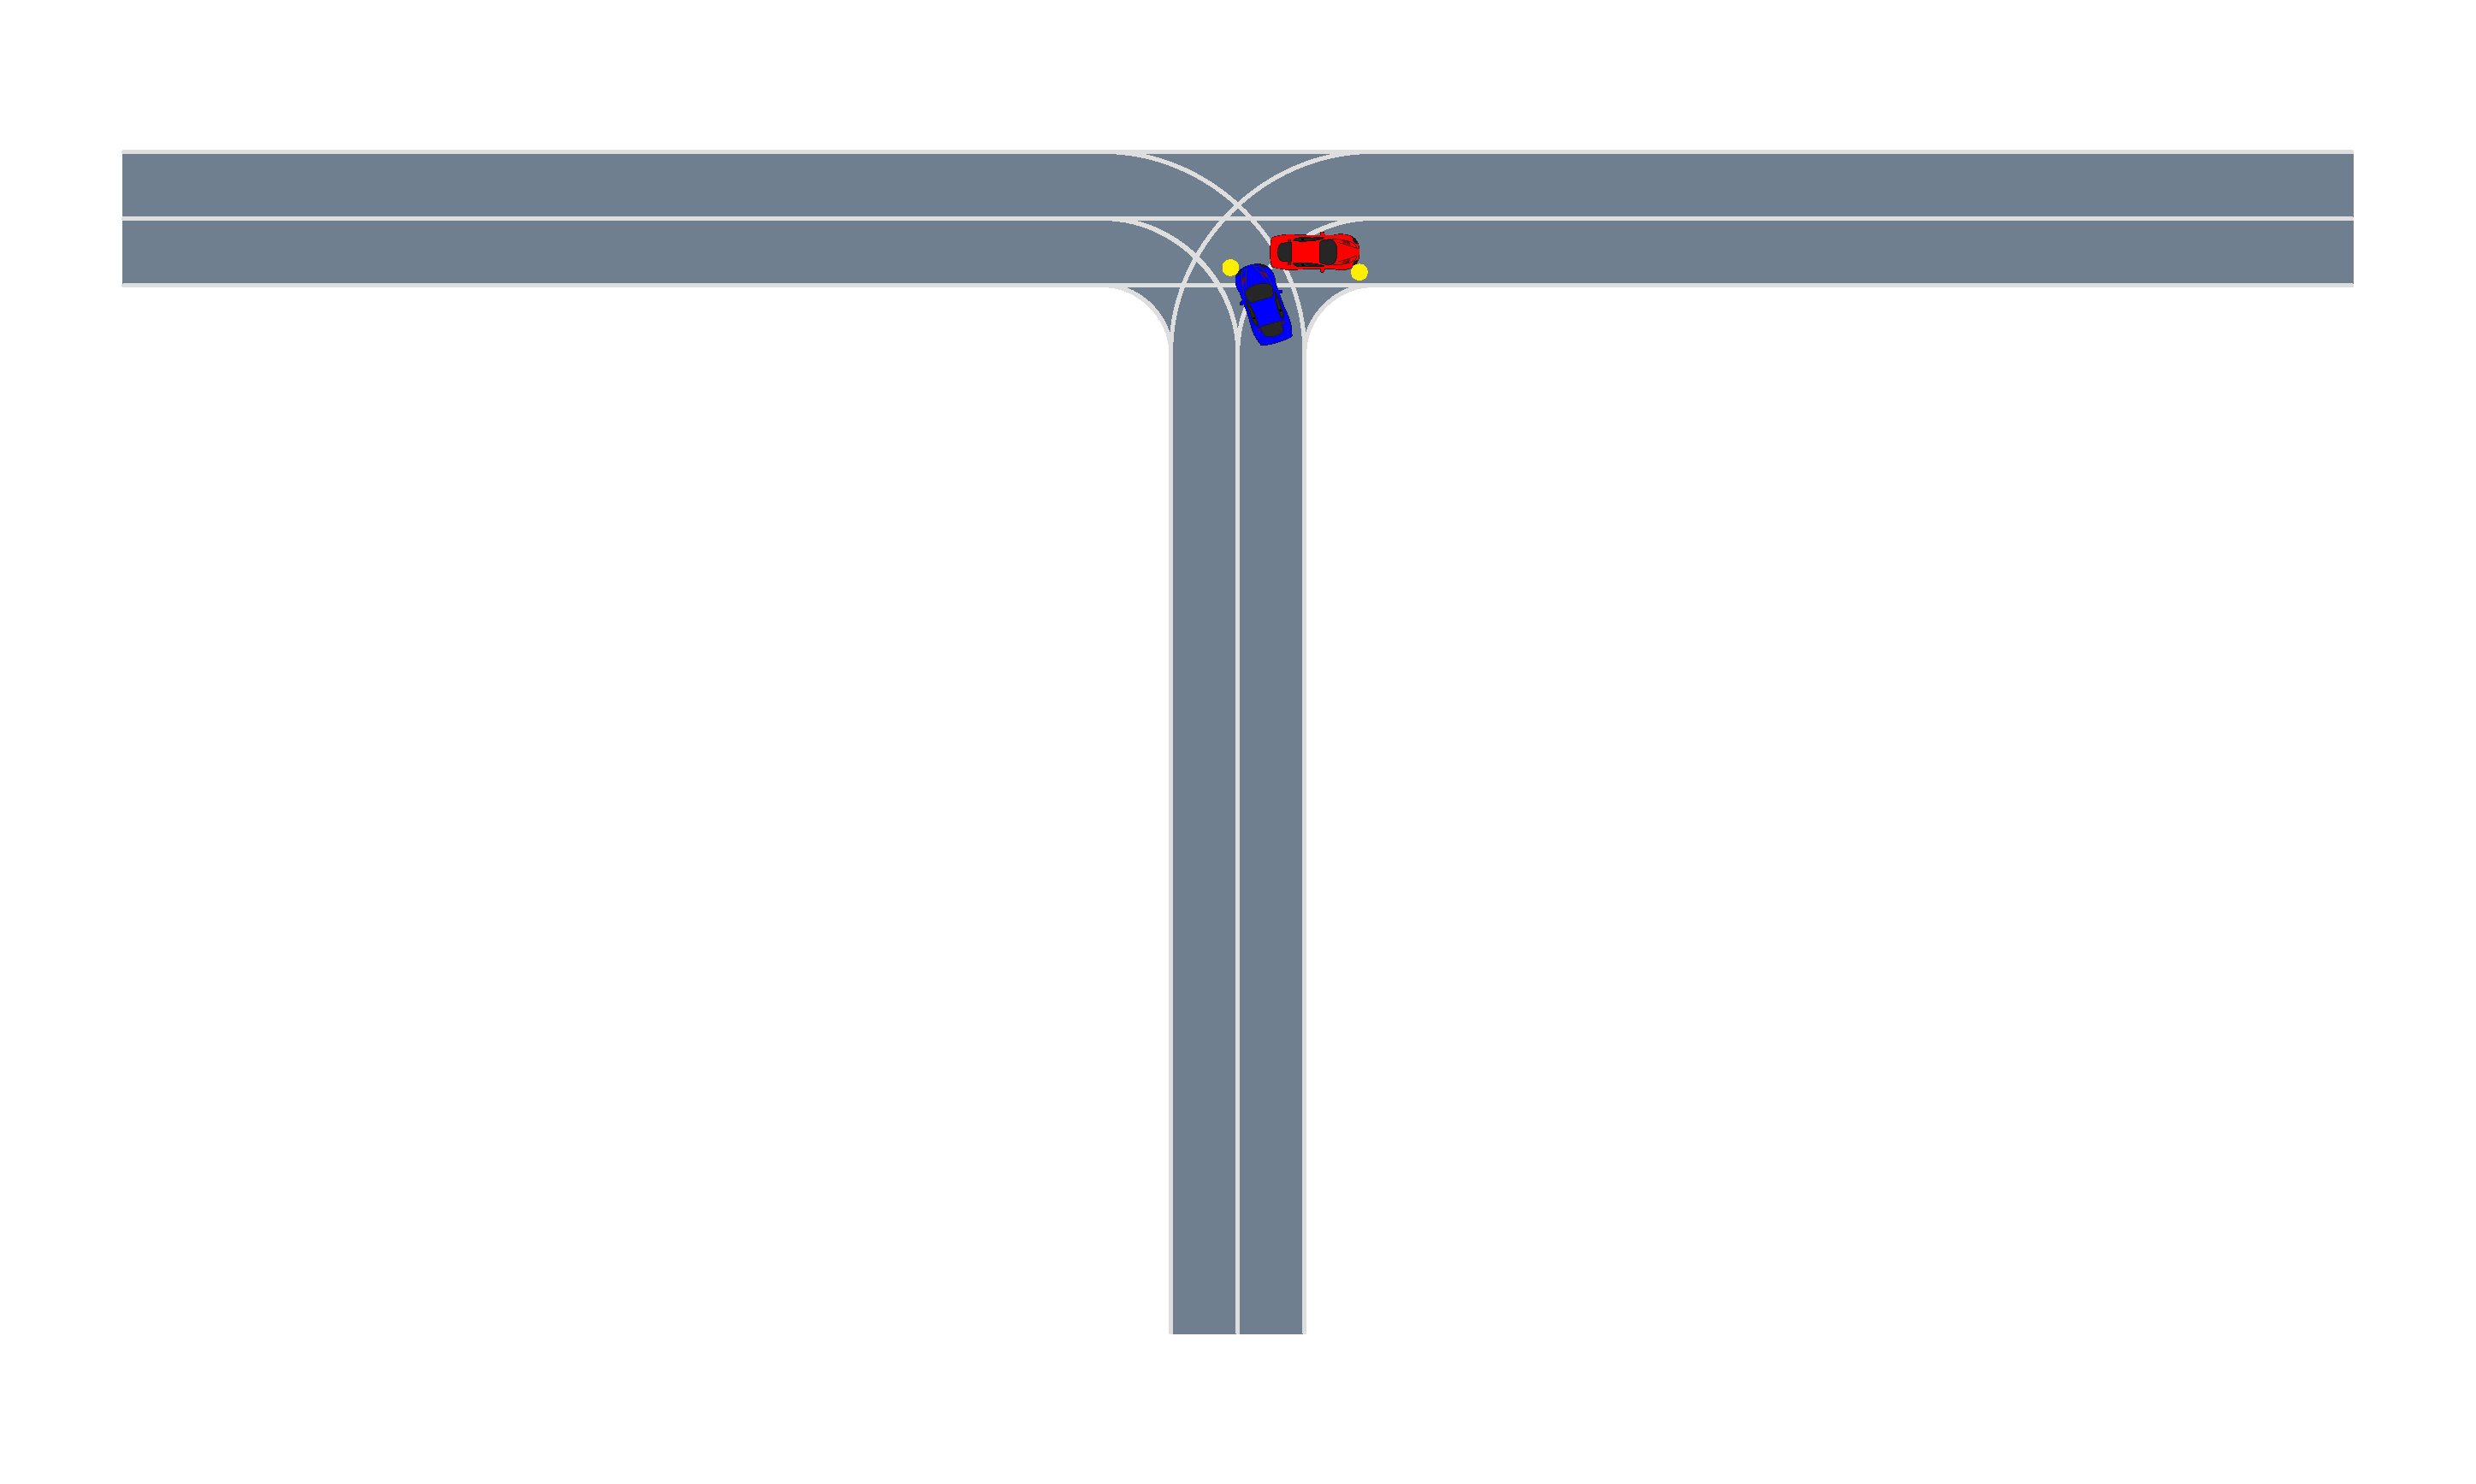
\includegraphics[width=0.9\textwidth, trim={10cm 16.5cm 22cm 0},clip]{figures/interpretable_validation/2car_res3_frame_10.pdf}
    \end{subfigure}
    \caption{Collision for LT3 at $t=(\SI{0}{s}, \SI{0.90}{s}, \SI{1.62}{s})$.}
    \label{fig:2car_LT3}
\end{figure}

% Sampling failure examples
One benefit to learning a failure description is the ability to produce many failure examples that have a shared temporal property. For example, we took the third failure description
\begin{equation}
    \square_{[0, .36]} B \lor d_{\rm maj}
\end{equation}
and use it to sample \num{10} failure trajectores. We plot the velocity vs. the position of the adversary for the failure examples in \cref{fig:2car_failure_samples}. We see that in the first two timesteps there is always a signification slowdown, but the trajectories then evolve stochastically before ending in a failure. 

\begin{figure}
    \centering
    \begin{tikzpicture}[/tikz/background rectangle/.style={fill={rgb,1:red,1.0;green,1.0;blue,1.0}, draw opacity={1.0}}, show background rectangle]
\begin{axis}[point meta max={nan}, point meta min={nan}, legend cell align={left}, title={Failure Examples}, title style={at={{(0.5,1)}}, anchor={south}, font={{\fontsize{14 pt}{18.2 pt}\selectfont}}, color={rgb,1:red,0.0;green,0.0;blue,0.0}, draw opacity={1.0}, rotate={0.0}}, legend style={color={rgb,1:red,0.0;green,0.0;blue,0.0}, draw opacity={1.0}, line width={1}, solid, fill={rgb,1:red,1.0;green,1.0;blue,1.0}, fill opacity={1.0}, text opacity={1.0}, font={{\fontsize{8 pt}{10.4 pt}\selectfont}}, at={(0.98, 0.98)}, anchor={north east}}, axis background/.style={fill={rgb,1:red,1.0;green,1.0;blue,1.0}, opacity={1.0}}, anchor={north west}, xshift={1.0mm}, yshift={-1.0mm}, width={0.9\textwidth}, height={75mm}, scaled x ticks={false}, xlabel={Position (m)}, x tick style={color={rgb,1:red,0.0;green,0.0;blue,0.0}, opacity={1.0}}, x tick label style={color={rgb,1:red,0.0;green,0.0;blue,0.0}, opacity={1.0}, rotate={0}}, xlabel style={at={(ticklabel cs:0.5)}, anchor=near ticklabel, font={{\fontsize{11 pt}{14.3 pt}\selectfont}}, color={rgb,1:red,0.0;green,0.0;blue,0.0}, draw opacity={1.0}, rotate={0.0}}, xmajorgrids={true}, xmin={13.987323701839703}, xmax={49.768552903503526}, xtick={{15.0,20.0,25.0,30.0,35.0,40.0,45.0}}, xticklabels={{$15$,$20$,$25$,$30$,$35$,$40$,$45$}}, xtick align={inside}, xticklabel style={font={{\fontsize{8 pt}{10.4 pt}\selectfont}}, color={rgb,1:red,0.0;green,0.0;blue,0.0}, draw opacity={1.0}, rotate={0.0}}, x grid style={color={rgb,1:red,0.0;green,0.0;blue,0.0}, draw opacity={0.1}, line width={0.5}, solid}, axis x line*={left}, x axis line style={color={rgb,1:red,0.0;green,0.0;blue,0.0}, draw opacity={1.0}, line width={1}, solid}, scaled y ticks={false}, ylabel={Velocity (m/s)}, y tick style={color={rgb,1:red,0.0;green,0.0;blue,0.0}, opacity={1.0}}, y tick label style={color={rgb,1:red,0.0;green,0.0;blue,0.0}, opacity={1.0}, rotate={0}}, ylabel style={at={(ticklabel cs:0.5)}, anchor=near ticklabel, font={{\fontsize{11 pt}{14.3 pt}\selectfont}}, color={rgb,1:red,0.0;green,0.0;blue,0.0}, draw opacity={1.0}, rotate={0.0}}, ymajorgrids={true}, ymin={14.291245239454959}, ymax={19.137148196909077}, ytick={{15.0,16.0,17.0,18.0,19.0}}, yticklabels={{$15$,$16$,$17$,$18$,$19$}}, ytick align={inside}, yticklabel style={font={{\fontsize{8 pt}{10.4 pt}\selectfont}}, color={rgb,1:red,0.0;green,0.0;blue,0.0}, draw opacity={1.0}, rotate={0.0}}, y grid style={color={rgb,1:red,0.0;green,0.0;blue,0.0}, draw opacity={0.1}, line width={0.5}, solid}, axis y line*={left}, y axis line style={color={rgb,1:red,0.0;green,0.0;blue,0.0}, draw opacity={1.0}, line width={1}, solid}]
    \addplot[color={rgb,1:red,0.0;green,0.0;blue,1.0}, name path={84166be1-6a89-49d6-a048-9e1a22b1249e}, draw opacity={1.0}, line width={1}, solid, mark={*}, mark size={3.0 pt}, mark repeat={1}, mark options={color={rgb,1:red,0.0;green,0.0;blue,0.0}, draw opacity={1.0}, fill={rgb,1:red,0.0;green,0.6056;blue,0.9787}, fill opacity={1.0}, line width={0.75}, rotate={0}, solid}]
        table[row sep={\\}]
        {
            \\
            15.0  19.0  \\
            16.413750005193712  18.700000138499274  \\
            17.805843770720298  18.42250027554303  \\
            19.177905511529506  18.165812812702534  \\
            20.531437624799587  17.928376874499595  \\
            21.867829829792683  17.708748591982943  \\
            23.18836762098077  17.505592506366014  \\
            24.494240081562243  17.31767310913995  \\
            25.786547114686964  17.143847774185936  \\
            27.066306124038974  16.983059141867678  \\
            28.33445820758427  16.834329752673526  \\
            29.591873886638986  16.696755022118868  \\
            30.839358387241507  16.569498327281664  \\
            32.077656543848796  16.451785848912685  \\
            33.30745733481509  16.342901910188566  \\
            34.529398066905216  16.24218427888138  \\
            35.74406824219072  16.149020395398797  \\
            36.95201315122341  16.062843845472937  \\
            38.15373719056824  15.983130537055924  \\
            39.34970692566019  15.909395732062732  \\
            40.540353933052984  15.841191131745054  \\
            41.72607742029766  15.778101861446366  \\
            42.90724664770689  15.71974420279963  \\
            44.084203187041794  15.665763512797708  \\
            45.257262995924336  15.615831390736673  \\
            46.4267183255533  15.569644066035693  \\
            47.592839508805184  15.526920820681225  \\
            48.75587660534323  15.48740175366673  \\
        }
        ;
    \addlegendentry {Nominal Trajectory}
    \addplot[color={rgb,1:red,0.502;green,0.502;blue,0.502}, name path={e3d3807d-edf7-4162-954e-8bf1da3be5ad}, draw opacity={0.5}, line width={1}, solid, mark={*}, mark size={3.0 pt}, mark repeat={1}, mark options={color={rgb,1:red,0.0;green,0.0;blue,0.0}, draw opacity={0.5}, fill={rgb,1:red,0.502;green,0.502;blue,0.502}, fill opacity={0.5}, line width={0.75}, rotate={0}, solid}]
        table[row sep={\\}]
        {
            \\
            15.0  19.0  \\
            16.40474174914094  18.459779977091955  \\
            17.789038445518017  18.454798592963453  \\
            19.158098690914922  18.0534746176207  \\
            20.504813967557304  17.85893275950952  \\
            21.829735011623196  17.47229508224764  \\
            23.13106574760941  17.229857877384717  \\
            24.41749871337977  17.07502120982499  \\
            25.69010752314532  16.861213717256287  \\
            26.95202302819319  16.789866417353625  \\
            28.21116165309647  16.787163580067286  \\
            29.46572853038647  16.667953147666072  \\
            30.701849874302013  16.295282690081645  \\
            31.919569203013886  16.177232742235013  \\
            33.134934786549366  16.232516152044425  \\
            34.35050465005139  16.1826802080096  \\
            35.55704639079141  15.991766211724348  \\
            36.7447803815312  15.681140208003223  \\
            37.924089403159286  15.767100368745641  \\
            39.10011696766464  15.593634684730404  \\
            40.26373091851866  15.436070671376756  \\
            41.415549042925356  15.279079312801818  \\
            42.55105074189209  15.000965992977864  \\
            43.67604711577298  14.998937310512503  \\
            44.80154331160483  15.0142945783369  \\
            45.922042562870026  14.865685455401664  \\
        }
        ;
    \addlegendentry {Sample Failure}
    \addplot[color={rgb,1:red,0.2422;green,0.6433;blue,0.3044}, name path={08e2d81b-3323-4341-9dd5-f12e5c00a838}, only marks, draw opacity={0.5}, line width={0}, solid, mark={diamond*}, mark size={7.5 pt}, mark repeat={1}, mark options={color={rgb,1:red,0.0;green,0.0;blue,0.0}, draw opacity={0.5}, fill={rgb,1:red,1.0;green,0.0;blue,0.0}, fill opacity={0.5}, line width={0.75}, rotate={0}, solid}]
        table[row sep={\\}]
        {
            \\
            45.922042562870026  14.865685455401664  \\
        }
        ;
    \addlegendentry {Collision}
    \addplot[color={rgb,1:red,0.502;green,0.502;blue,0.502}, name path={4a48a594-8c24-43a9-a9be-5cb6dc9b275c}, draw opacity={0.5}, line width={1}, solid, mark={*}, mark size={3.0 pt}, mark repeat={1}, mark options={color={rgb,1:red,0.0;green,0.0;blue,0.0}, draw opacity={0.5}, fill={rgb,1:red,0.502;green,0.502;blue,0.502}, fill opacity={0.5}, line width={0.75}, rotate={0}, solid}, forget plot]
        table[row sep={\\}]
        {
            \\
            15.0  19.0  \\
            16.40551737013116  18.480463203497898  \\
            17.788650426267967  18.40308496015031  \\
            19.160271772892663  18.173484283174883  \\
            20.521600908482554  18.128625999222244  \\
            21.863456214146254  17.65418215180972  \\
            23.181458444407458  17.492543988489064  \\
            24.48575289510888  17.28864136354893  \\
            25.777122459872544  17.147880363482116  \\
            27.058191198995253  17.01395267979015  \\
            28.325397439750382  16.778213740346654  \\
            29.572782801914  16.485395917349802  \\
            30.804738582867135  16.366758241400575  \\
            32.025174864693014  16.17820927395626  \\
            33.23803483719254  16.1647233260311  \\
            34.44672733848929  16.06707670854898  \\
            35.64089371907109  15.777360106965604  \\
            36.812701817781004  15.470855858632135  \\
            37.982724575727225  15.729751019933689  \\
            39.1610874395641  15.693258682382929  \\
            40.33282166351773  15.552987289713819  \\
            41.502550410338415  15.63977929217114  \\
            42.67643510539657  15.663812576046368  \\
            43.854230585151974  15.744066884097638  \\
            45.02574770380233  15.496389613245226  \\
            46.18751423701599  15.484051272452263  \\
        }
        ;
    \addplot[color={rgb,1:red,0.6755;green,0.5557;blue,0.0942}, name path={06cbed38-6b6e-4d31-9074-a78605af5b5a}, only marks, draw opacity={0.5}, line width={0}, solid, mark={diamond*}, mark size={7.5 pt}, mark repeat={1}, mark options={color={rgb,1:red,0.0;green,0.0;blue,0.0}, draw opacity={0.5}, fill={rgb,1:red,1.0;green,0.0;blue,0.0}, fill opacity={0.5}, line width={0.75}, rotate={0}, solid}, forget plot]
        table[row sep={\\}]
        {
            \\
            46.18751423701599  15.484051272452263  \\
        }
        ;
    \addplot[color={rgb,1:red,0.502;green,0.502;blue,0.502}, name path={a3d385c6-27a8-46c8-9d45-1ef69d834126}, draw opacity={0.5}, line width={1}, solid, mark={*}, mark size={3.0 pt}, mark repeat={1}, mark options={color={rgb,1:red,0.0;green,0.0;blue,0.0}, draw opacity={0.5}, fill={rgb,1:red,0.502;green,0.502;blue,0.502}, fill opacity={0.5}, line width={0.75}, rotate={0}, solid}, forget plot]
        table[row sep={\\}]
        {
            \\
            15.0  19.0  \\
            16.40499824001176  18.466619733647146  \\
            17.78268497332361  18.27169315466888  \\
            19.14575060124614  18.076723589931813  \\
            20.489615673149657  17.75967832749539  \\
            21.813048364713712  17.53186011421277  \\
            23.116104037821167  17.21629116865273  \\
            24.40135212943668  17.056991274427695  \\
            25.6751134833658  16.90997816368211  \\
            26.933846941720713  16.656247392448904  \\
            28.176680234174796  16.48597373965987  \\
            29.40356258665979  16.230888993273254  \\
            30.608276124006455  15.894805335971233  \\
            31.799921004113767  15.882391466890526  \\
            32.99130022558573  15.88772110569532  \\
            34.175191988032225  15.682725892877814  \\
            35.34775189163868  15.585538203294297  \\
            36.514179088360244  15.519187042614135  \\
            37.67574315258225  15.455854669972712  \\
            38.836674527673964  15.502315332472984  \\
            39.9989542461833  15.491810494442626  \\
            41.153705614463455  15.301559326361385  \\
            42.30233391586778  15.328528711087234  \\
            43.45852173882554  15.503146567786336  \\
            44.61817726696441  15.421000849250282  \\
            45.7821869911995  15.619258463685613  \\
        }
        ;
    \addplot[color={rgb,1:red,0.9308;green,0.3675;blue,0.5758}, name path={92ebb41f-bc17-4087-aa78-67b6feba2468}, only marks, draw opacity={0.5}, line width={0}, solid, mark={diamond*}, mark size={7.5 pt}, mark repeat={1}, mark options={color={rgb,1:red,0.0;green,0.0;blue,0.0}, draw opacity={0.5}, fill={rgb,1:red,1.0;green,0.0;blue,0.0}, fill opacity={0.5}, line width={0.75}, rotate={0}, solid}, forget plot]
        table[row sep={\\}]
        {
            \\
            45.7821869911995  15.619258463685613  \\
        }
        ;
    \addplot[color={rgb,1:red,0.502;green,0.502;blue,0.502}, name path={60988a01-bdf7-4173-a150-1a114cc86b77}, draw opacity={0.5}, line width={1}, solid, mark={*}, mark size={3.0 pt}, mark repeat={1}, mark options={color={rgb,1:red,0.0;green,0.0;blue,0.0}, draw opacity={0.5}, fill={rgb,1:red,0.502;green,0.502;blue,0.502}, fill opacity={0.5}, line width={0.75}, rotate={0}, solid}, forget plot]
        table[row sep={\\}]
        {
            \\
            15.0  19.0  \\
            16.404268988125573  18.447173016682182  \\
            17.773090118119065  18.054723783144283  \\
            19.117330472486863  17.79168566666362  \\
            20.447724387582902  17.685485402564087  \\
            21.76761050534366  17.511477737722807  \\
            23.07300636169939  17.299078431763345  \\
            24.365481032029347  17.166912777035435  \\
            25.65324628445873  17.173493954414816  \\
            26.927465267495077  16.80567892655441  \\
            28.17945002683995  16.580581322642292  \\
            29.40995601944284  16.232911813434683  \\
            30.62700166551309  16.221638748438714  \\
            31.83592655433597  16.01635828683799  \\
            33.03702474838608  16.012926887831714  \\
            34.231927728254064  15.851152575314426  \\
            35.42135688954377  15.86695839241121  \\
            36.60689772905957  15.74746399467668  \\
            37.79688750910592  15.98559680655936  \\
            38.99380630691432  15.932237801664753  \\
            40.189054035175346  15.94103495196252  \\
            41.382099285276574  15.8735050507369  \\
            42.56658315786362  15.712731551584328  \\
            43.74776689890326  15.785501542806113  \\
            44.922625020073546  15.5440483550683  \\
            46.093618266162686  15.682438207308675  \\
        }
        ;
    \addplot[color={rgb,1:red,0.0;green,0.6643;blue,0.553}, name path={13569532-5e6b-4b48-bb0c-df17d8ff93ea}, only marks, draw opacity={0.5}, line width={0}, solid, mark={diamond*}, mark size={7.5 pt}, mark repeat={1}, mark options={color={rgb,1:red,0.0;green,0.0;blue,0.0}, draw opacity={0.5}, fill={rgb,1:red,1.0;green,0.0;blue,0.0}, fill opacity={0.5}, line width={0.75}, rotate={0}, solid}, forget plot]
        table[row sep={\\}]
        {
            \\
            46.093618266162686  15.682438207308675  \\
        }
        ;
    \addplot[color={rgb,1:red,0.502;green,0.502;blue,0.502}, name path={17ac5c39-0314-41a4-bfb2-832f5f9874a0}, draw opacity={0.5}, line width={1}, solid, mark={*}, mark size={3.0 pt}, mark repeat={1}, mark options={color={rgb,1:red,0.0;green,0.0;blue,0.0}, draw opacity={0.5}, fill={rgb,1:red,0.502;green,0.502;blue,0.502}, fill opacity={0.5}, line width={0.75}, rotate={0}, solid}, forget plot]
        table[row sep={\\}]
        {
            \\
            15.0  19.0  \\
            16.403935424832365  18.43827799552994  \\
            17.7677573564156  17.930306846689643  \\
            19.092164850034326  17.387226316476404  \\
            20.390004074727116  17.22181967533139  \\
            21.672305340093068  16.97288073442735  \\
            22.94648140308987  17.00514761215402  \\
            24.215646896698374  16.839265550739473  \\
            25.470066029225872  16.611911316660514  \\
            26.70080016015948  16.207665508235714  \\
            27.888907379763634  15.475193681208385  \\
            29.05046943744958  15.499794523750078  \\
            30.20526723985817  15.29481354047894  \\
            31.344175214342567  15.07606577910496  \\
            32.48528899364154  15.353635002200921  \\
            33.63709915521122  15.361302639657124  \\
            34.78894063386398  15.35447012441651  \\
            35.94158889454739  15.382816827141072  \\
            37.08806292131855  15.189823886756617  \\
            38.22755761179751  15.196701192682172  \\
            39.36260950989953  15.071349423371645  \\
            40.481689149884495  14.770774309560839  \\
            41.59742292848273  14.982126453058711  \\
            42.713340775700516  14.775682806082195  \\
            43.83060247107123  15.017962403803462  \\
            44.95773186803933  15.038821515345832  \\
            46.06275242872845  14.428393436364038  \\
        }
        ;
    \addplot[color={rgb,1:red,0.0;green,0.6609;blue,0.7982}, name path={6637ad73-ef9c-485a-bf29-291059c40958}, only marks, draw opacity={0.5}, line width={0}, solid, mark={diamond*}, mark size={7.5 pt}, mark repeat={1}, mark options={color={rgb,1:red,0.0;green,0.0;blue,0.0}, draw opacity={0.5}, fill={rgb,1:red,1.0;green,0.0;blue,0.0}, fill opacity={0.5}, line width={0.75}, rotate={0}, solid}, forget plot]
        table[row sep={\\}]
        {
            \\
            46.06275242872845  14.428393436364038  \\
        }
        ;
    \addplot[color={rgb,1:red,0.502;green,0.502;blue,0.502}, name path={0cb8e76e-a2c1-4f07-bced-98275e441ad3}, draw opacity={0.5}, line width={1}, solid, mark={*}, mark size={3.0 pt}, mark repeat={1}, mark options={color={rgb,1:red,0.0;green,0.0;blue,0.0}, draw opacity={0.5}, fill={rgb,1:red,0.502;green,0.502;blue,0.502}, fill opacity={0.5}, line width={0.75}, rotate={0}, solid}, forget plot]
        table[row sep={\\}]
        {
            \\
            15.0  19.0  \\
            16.404301210601172  18.448032282698176  \\
            17.772501097790325  18.037298042345903  \\
            19.11839016155035  17.853076991254795  \\
            20.453938048965526  17.761533339816513  \\
            21.776194005507076  17.498625501291468  \\
            23.074011580179544  17.109843156641052  \\
            24.349160550198164  16.894129377188772  \\
            25.60891052030688  16.69920315904352  \\
            26.846565060863668  16.304917922470946  \\
            28.072154068055134  16.377455602634807  \\
            29.286531553267064  16.005944003016687  \\
            30.47388618082841  15.656846065285848  \\
            31.650275474088563  15.713535088318228  \\
            32.825578806552635  15.627887110723714  \\
            33.98585454059853  15.31279913050025  \\
            35.135798233065266  15.352366001946013  \\
            36.287369280794664  15.356195270837876  \\
            37.433572475256  15.209223248131128  \\
            38.566330726880274  14.997663461849514  \\
            39.68395957950869  14.805772608241586  \\
            40.79674671572754  14.86855102426113  \\
            41.91290481601966  14.895664983528896  \\
            43.03537109807628  15.036769204647626  \\
            44.1641958273941  15.065223577160841  \\
            45.28712535169018  14.879563737401186  \\
        }
        ;
    \addplot[color={rgb,1:red,0.38;green,0.5511;blue,0.9665}, name path={334d23a8-a084-44fb-88d0-2ff2d0f21242}, only marks, draw opacity={0.5}, line width={0}, solid, mark={diamond*}, mark size={7.5 pt}, mark repeat={1}, mark options={color={rgb,1:red,0.0;green,0.0;blue,0.0}, draw opacity={0.5}, fill={rgb,1:red,1.0;green,0.0;blue,0.0}, fill opacity={0.5}, line width={0.75}, rotate={0}, solid}, forget plot]
        table[row sep={\\}]
        {
            \\
            45.28712535169018  14.879563737401186  \\
        }
        ;
    \addplot[color={rgb,1:red,0.502;green,0.502;blue,0.502}, name path={991da9d0-9a91-4e0a-8da3-09e2bbc57c87}, draw opacity={0.5}, line width={1}, solid, mark={*}, mark size={3.0 pt}, mark repeat={1}, mark options={color={rgb,1:red,0.0;green,0.0;blue,0.0}, draw opacity={0.5}, fill={rgb,1:red,0.502;green,0.502;blue,0.502}, fill opacity={0.5}, line width={0.75}, rotate={0}, solid}, forget plot]
        table[row sep={\\}]
        {
            \\
            15.0  19.0  \\
            16.40398139713427  18.439503923580816  \\
            17.78077637026484  18.27502869323431  \\
            19.135247445147996  17.844199970316556  \\
            20.45657968740924  17.39132648998323  \\
            21.752944799132067  17.178409822625493  \\
            23.032000116944044  16.92973198569393  \\
            24.300168825408928  16.88810024003633  \\
            25.570606719661214  16.99024360669141  \\
            26.850338228844144  17.135929971520067  \\
            28.130891803558058  17.01216535418433  \\
            29.396794362770272  16.745236224808025  \\
            30.652973180828084  16.752865590067024  \\
            31.90526097722546  16.641475647196216  \\
            33.15274757139936  16.624833530774538  \\
            34.393532004984735  16.462751364835555  \\
            35.625394746493434  16.386921742063006  \\
            36.844822549313676  16.131152999810105  \\
            38.05562294846094  16.156857644116982  \\
            39.26159114150862  16.002294170487676  \\
            40.4505401976906  15.70301399436522  \\
            41.6258373905106  15.638244480834619  \\
            42.79595645079953  15.564930460203675  \\
            43.96557471680763  15.624889966678946  \\
            45.143909629462975  15.797374370796968  \\
            46.32256564931475  15.633452825250215  \\
        }
        ;
    \addplot[color={rgb,1:red,0.8684;green,0.396;blue,0.7135}, name path={bf8cc7f9-79a9-4a04-9f67-970bc3da18eb}, only marks, draw opacity={0.5}, line width={0}, solid, mark={diamond*}, mark size={7.5 pt}, mark repeat={1}, mark options={color={rgb,1:red,0.0;green,0.0;blue,0.0}, draw opacity={0.5}, fill={rgb,1:red,1.0;green,0.0;blue,0.0}, fill opacity={0.5}, line width={0.75}, rotate={0}, solid}, forget plot]
        table[row sep={\\}]
        {
            \\
            46.32256564931475  15.633452825250215  \\
        }
        ;
    \addplot[color={rgb,1:red,0.502;green,0.502;blue,0.502}, name path={47644102-7c9d-4ce9-a713-b1e48c50c93f}, draw opacity={0.5}, line width={1}, solid, mark={*}, mark size={3.0 pt}, mark repeat={1}, mark options={color={rgb,1:red,0.0;green,0.0;blue,0.0}, draw opacity={0.5}, fill={rgb,1:red,0.502;green,0.502;blue,0.502}, fill opacity={0.5}, line width={0.75}, rotate={0}, solid}, forget plot]
        table[row sep={\\}]
        {
            \\
            15.0  19.0  \\
            16.403800418429043  18.434677824774695  \\
            17.776387635651172  18.167647967815405  \\
            19.132340653883897  17.991099185057244  \\
            20.481016342204978  17.973585836838225  \\
            21.818861742824048  17.702291513003683  \\
            23.14230669155296  17.58957378643394  \\
            24.4566980927128  17.46086357782845  \\
            25.76048519036906  17.30679235967185  \\
            27.053848648722806  17.182899863094722  \\
            28.330732507872092  16.867336380886243  \\
            29.582519352559682  16.513646144116148  \\
            30.823152403521608  16.569901881535273  \\
            32.06946681111214  16.665148987545763  \\
            33.31680028214692  16.59707690671496  \\
            34.56645003366615  16.726916467131133  \\
            35.80529056308246  16.308830983970406  \\
            37.029270100563906  16.330623348868254  \\
            38.24562250006264  16.10544063776455  \\
            39.453153200256374  16.095378034068414  \\
            40.660340210816344  16.09627558086415  \\
            41.867676218512486  16.099351291033013  \\
            43.07440218306982  16.080007763829276  \\
            44.26749245541237  15.735732831972202  \\
            45.45373424281555  15.89738149877915  \\
            46.64697995901489  15.922504266536656  \\
        }
        ;
    \addplot[color={rgb,1:red,0.0;green,0.6056;blue,0.9787}, name path={b7d402a1-7ad0-45a2-b69f-706465dcbea4}, only marks, draw opacity={0.5}, line width={0}, solid, mark={diamond*}, mark size={7.5 pt}, mark repeat={1}, mark options={color={rgb,1:red,0.0;green,0.0;blue,0.0}, draw opacity={0.5}, fill={rgb,1:red,1.0;green,0.0;blue,0.0}, fill opacity={0.5}, line width={0.75}, rotate={0}, solid}, forget plot]
        table[row sep={\\}]
        {
            \\
            46.64697995901489  15.922504266536656  \\
        }
        ;
    \addplot[color={rgb,1:red,0.502;green,0.502;blue,0.502}, name path={17e7c574-f5f4-4a8c-8c4b-97eccc16b1b5}, draw opacity={0.5}, line width={1}, solid, mark={*}, mark size={3.0 pt}, mark repeat={1}, mark options={color={rgb,1:red,0.0;green,0.0;blue,0.0}, draw opacity={0.5}, fill={rgb,1:red,0.502;green,0.502;blue,0.502}, fill opacity={0.5}, line width={0.75}, rotate={0}, solid}, forget plot]
        table[row sep={\\}]
        {
            \\
            15.0  19.0  \\
            16.405168936668865  18.471171644503304  \\
            17.782436921756236  18.255974624493305  \\
            19.14977195970778  18.206293054214566  \\
            20.50147806197065  17.83920300612869  \\
            21.829926556600245  17.586090183993797  \\
            23.139819731591686  17.344394482444635  \\
            24.42820831064997  17.01263429244301  \\
            25.697478042040174  16.83455854462893  \\
            26.953425522652115  16.657374271689456  \\
            28.199083212408578  16.560164121816143  \\
            29.43404990523655  16.372281020262978  \\
            30.655060037896646  16.187989184006284  \\
            31.868674049043854  16.175051113252696  \\
            33.07043898385482  15.87201381503981  \\
            34.26297971323073  15.92907230165094  \\
            35.460947737051384  16.016741666899833  \\
            36.66574129360026  16.111086507737006  \\
            37.867882802210495  15.946020388535858  \\
            39.071233930826935  16.143343041235877  \\
            40.28323562306566  16.176702085130128  \\
            41.4964476199784  16.175617832543008  \\
            42.699984864470565  15.918708687248138  \\
            43.89590851510906  15.972588663111864  \\
            45.091871109474575  15.919747186635014  \\
            46.290197672514914  16.035627827773958  \\
        }
        ;
    \addplot[color={rgb,1:red,0.2422;green,0.6433;blue,0.3044}, name path={22303187-bf6a-4020-a23c-e5f6a8d53941}, only marks, draw opacity={0.5}, line width={0}, solid, mark={diamond*}, mark size={7.5 pt}, mark repeat={1}, mark options={color={rgb,1:red,0.0;green,0.0;blue,0.0}, draw opacity={0.5}, fill={rgb,1:red,1.0;green,0.0;blue,0.0}, fill opacity={0.5}, line width={0.75}, rotate={0}, solid}, forget plot]
        table[row sep={\\}]
        {
            \\
            46.290197672514914  16.035627827773958  \\
        }
        ;
    \addplot[color={rgb,1:red,0.502;green,0.502;blue,0.502}, name path={ef68dc01-165b-4d06-9d51-7ae4ab7a0200}, draw opacity={0.5}, line width={1}, solid, mark={*}, mark size={3.0 pt}, mark repeat={1}, mark options={color={rgb,1:red,0.0;green,0.0;blue,0.0}, draw opacity={0.5}, fill={rgb,1:red,0.502;green,0.502;blue,0.502}, fill opacity={0.5}, line width={0.75}, rotate={0}, solid}, forget plot]
        table[row sep={\\}]
        {
            \\
            15.0  19.0  \\
            16.40546916351651  18.479177693773845  \\
            17.779649273602832  18.165625241861363  \\
            19.13612223887631  18.006987165431383  \\
            20.48372811260427  17.929169467314175  \\
            21.836514038708142  18.14512189545581  \\
            23.19136896306497  17.984342754059675  \\
            24.535297677787042  17.853756305195525  \\
            25.86371054566276  17.5705868381569  \\
            27.172301248024688  17.32516522482788  \\
            28.469034918115057  17.25439931091518  \\
            29.753736887601733  17.004319875396263  \\
            31.01984184458203  16.758478977411627  \\
            32.27064991980246  16.59640302846649  \\
            33.507933557724826  16.39782731612999  \\
            34.734316365326386  16.305714219911643  \\
            35.95155574668264  16.154002616255056  \\
            37.15685656000489  15.987352405671704  \\
            38.354409282850305  15.947386870206051  \\
            39.54833666354045  15.890676614864383  \\
            40.7418535369532  15.936440009475705  \\
            41.93061213331934  15.763789226954849  \\
            43.10862493626067  15.649885518147075  \\
            44.276915116138994  15.504519278608273  \\
            45.44213012980147  15.567881085724368  \\
            46.61580161031636  15.730025061339411  \\
        }
        ;
    \addplot[color={rgb,1:red,0.6755;green,0.5557;blue,0.0942}, name path={e9ca29d6-c5cd-4019-ac75-3b271a1f600c}, only marks, draw opacity={0.5}, line width={0}, solid, mark={diamond*}, mark size={7.5 pt}, mark repeat={1}, mark options={color={rgb,1:red,0.0;green,0.0;blue,0.0}, draw opacity={0.5}, fill={rgb,1:red,1.0;green,0.0;blue,0.0}, fill opacity={0.5}, line width={0.75}, rotate={0}, solid}, forget plot]
        table[row sep={\\}]
        {
            \\
            46.61580161031636  15.730025061339411  \\
        }
        ;
\end{axis}
\end{tikzpicture}

    \caption{Sample failures that satisfy $\square_{[0, 0.36]} B \lor d_{\rm maj}$}
    \label{fig:2car_failure_samples}
\end{figure}


\subsection{Pedestrian in Crosswalk}

In the first set of experiments involving the pedestrian in a crosswalk we use the full STL grammar (\cref{eq:stl_grammar}) to sample expressions. The pedestrian accelerations in each direction were modeled as zero-mean Gaussian processes with a squared exponential kernel with parameters $\ell = 4$ and $\sigma^2 = 0.5$. The noise was modeled iid as zero mean Gaussians with parameters $\sigma_{r_x} = \sigma_{r_y} = 0.2$ and $\sigma_{v} = 0.5$. The initial condition for the vehicle was ($r_x^{\rm veh}$, $v_x^{\rm veh}$) = (\SI{9.23}{m}, \SI{18.72}{m/s}) and for the pedestrian ($r^{\rm ped}_x$, $r^{\rm ped}_y$, $v^{\rm ped}_x$, $v^{\rm ped}_y$) = (\SI{25}{m}, \SI{-3.83}{m}, \SI{0.83}{m/s}, \SI{0}{m/s}).

The interpretable validation algorithm produced the failure description
\begin{equation}
\square_{[1,3]}\left((1.68 \leq \delta a_y \leq 2.69) \land (\delta a_x \geq 0.34) \land (\delta n_y \geq 0.13) \right) \label{eq:failure_description_pedstl} \text{.}
\end{equation}
In words, there is a positive lateral and longitudinal acceleration of the pedestrian early in the trajectory, combined with a positive bias in the noise. The vehicle initially does not think the pedestrian will reach the road before it passes, but the sudden change in pedestrain velocity leads to this being a miscalculation and a collision occurs. Ten example failure trajectories were generated from the failure description and plotted in \cref{fig:ped_stl_sample_failures}.

The failure rate and log-likelihood results for the failure description and the baseline are shown in \cref{tab:ped_results_stl}.  We notice that although the cross entropy methods can produce a similarly high rate of failures as the failure description, the log probability of those failures is significantly smaller. The failure description produces failure trajectories nearly 100\% of the time while retaining a log-likelihood similar to failures found through Monte Carlo sampling. 

\begin{table}
    \centering
    \caption{Comparison of interpretable validation with STL grammar to baselines for pedestrian scenario.}
    \label{tab:ped_results_stl}
    \begin{tabular}{@{}llll@{}} 
        \toprule
        \textbf{Method} & \textbf{Fail Rate} & \textbf{Log-Likelihood} \\
        \midrule
        Monte Carlo & $0.003 \pm 0.002$ & $2.365 \pm 0.235$  \\
        Cross entropy method (IID) & $0.865 \pm 0.011$ & $\num{-9.317e4} \pm \num{2.824e3}$\\
        Cross entropy method (Trajectory) & $0.989 \pm 0.003$ & $-11.308 \pm 1.980$ \\
        Interpretable validation & $0.960 \pm 0.006$ & $1.835 \pm 0.218$ \\
        \bottomrule
    \end{tabular}
\end{table}

\begin{figure}
    \begin{tikzpicture}[/tikz/background rectangle/.style={fill={rgb,1:red,1.0;green,1.0;blue,1.0}, draw opacity={1.0}}, show background rectangle]
\begin{axis}[point meta max={nan}, point meta min={nan}, legend cell align={left}, title={}, title style={at={{(0.5,1)}}, anchor={south}, font={{\fontsize{14 pt}{18.2 pt}\selectfont}}, color={rgb,1:red,0.0;green,0.0;blue,0.0}, draw opacity={0.0}, rotate={0.0}}, legend style={color={rgb,1:red,0.0;green,0.0;blue,0.0}, draw opacity={0.0}, line width={1}, solid, fill={rgb,1:red,1.0;green,1.0;blue,1.0}, fill opacity={0.0}, text opacity={1.0}, font={{\fontsize{8 pt}{10.4 pt}\selectfont}}, at={(0.98, 0.98)}, anchor={north east}}, axis background/.style={fill={rgb,1:red,1.0;green,1.0;blue,1.0}, opacity={1.0}}, anchor={north west}, xshift={10.0mm}, yshift={-1.0mm}, width={0.9\textwidth}, height={75mm}, scaled x ticks={false}, xlabel={x-position (m)}, x tick style={color={rgb,1:red,0.0;green,0.0;blue,0.0}, opacity={1.0}}, x tick label style={color={rgb,1:red,0.0;green,0.0;blue,0.0}, opacity={1.0}, rotate={0}}, xlabel style={at={(ticklabel cs:0.5)}, anchor=near ticklabel, font={{\fontsize{11 pt}{14.3 pt}\selectfont}}, color={rgb,1:red,0.0;green,0.0;blue,0.0}, draw opacity={1.0}, rotate={0.0}}, xmajorgrids={true}, xmin={24.977603333639614}, xmax={25.768952211706626}, xtick={{25.0,25.200000000000003,25.400000000000002,25.6}}, xticklabels={{$25.0$,$25.2$,$25.4$,$25.6$}}, xtick align={inside}, xticklabel style={font={{\fontsize{8 pt}{10.4 pt}\selectfont}}, color={rgb,1:red,0.0;green,0.0;blue,0.0}, draw opacity={1.0}, rotate={0.0}}, x grid style={color={rgb,1:red,0.0;green,0.0;blue,0.0}, draw opacity={0.1}, line width={0.5}, solid}, axis x line*={left}, x axis line style={color={rgb,1:red,0.0;green,0.0;blue,0.0}, draw opacity={1.0}, line width={1}, solid}, scaled y ticks={false}, ylabel={y-position (m)}, y tick style={color={rgb,1:red,0.0;green,0.0;blue,0.0}, opacity={1.0}}, y tick label style={color={rgb,1:red,0.0;green,0.0;blue,0.0}, opacity={1.0}, rotate={0}}, ylabel style={at={(ticklabel cs:0.5)}, anchor=near ticklabel, font={{\fontsize{11 pt}{14.3 pt}\selectfont}}, color={rgb,1:red,0.0;green,0.0;blue,0.0}, draw opacity={1.0}, rotate={0.0}}, ymajorgrids={true}, ymin={-3.908896636923623}, ymax={-1.084312781835062}, ytick={{-3.5,-3.0,-2.5,-2.0,-1.5}}, yticklabels={{$-3.5$,$-3.0$,$-2.5$,$-2.0$,$-1.5$}}, ytick align={inside}, yticklabel style={font={{\fontsize{8 pt}{10.4 pt}\selectfont}}, color={rgb,1:red,0.0;green,0.0;blue,0.0}, draw opacity={1.0}, rotate={0.0}}, y grid style={color={rgb,1:red,0.0;green,0.0;blue,0.0}, draw opacity={0.1}, line width={0.5}, solid}, axis y line*={left}, y axis line style={color={rgb,1:red,0.0;green,0.0;blue,0.0}, draw opacity={1.0}, line width={1}, solid}]
    \addplot[color={rgb,1:red,0.0;green,0.0;blue,1.0}, name path={ac9afe6d-2d48-4632-9e29-005b532a371c}, draw opacity={1.0}, line width={1}, solid, mark={*}, mark size={3.0 pt}, mark repeat={1}, mark options={color={rgb,1:red,0.0;green,0.0;blue,0.0}, draw opacity={1.0}, fill={rgb,1:red,0.0;green,0.6056;blue,0.9787}, fill opacity={1.0}, line width={0.75}, rotate={0}, solid}]
        table[row sep={\\}]
        {
            \\
            25.0  -3.8289555844211165  \\
            25.0  -3.6624117250408963  \\
            25.0  -3.4958678656606734  \\
            25.0  -3.3293240062804514  \\
            25.0  -3.1627801469002295  \\
            25.0  -2.9962362875200066  \\
            25.0  -2.8296924281397846  \\
            25.0  -2.6631485687595626  \\
            25.0  -2.4966047093793406  \\
            25.0  -2.330060849999117  \\
            25.0  -2.163516990618895  \\
            25.0  -1.9969731312386738  \\
            25.0  -1.8304292718584527  \\
            25.0  -1.6638854124782316  \\
            25.0  -1.4973415530980105  \\
            25.0  -1.3307976937177894  \\
            25.0  -1.1642538343375683  \\
        }
        ;
    \addlegendentry {Nominal Trajectory}
    \addplot[color={rgb,1:red,0.502;green,0.502;blue,0.502}, name path={97e6e2cb-6ad5-47bc-8e16-7569c326e3f0}, draw opacity={0.5}, line width={1}, solid, mark={*}, mark size={3.0 pt}, mark repeat={1}, mark options={color={rgb,1:red,0.0;green,0.0;blue,0.0}, draw opacity={0.5}, fill={rgb,1:red,0.502;green,0.502;blue,0.502}, fill opacity={0.5}, line width={0.75}, rotate={0}, solid}]
        table[row sep={\\}]
        {
            \\
            25.0  -3.8289555844211165  \\
            25.01520734721681  -3.6236422360557894  \\
            25.05705972144588  -3.3435663156467346  \\
            25.117785544101586  -2.9924318637944944  \\
            25.190370078201195  -2.5705205899400427  \\
            25.270467354564918  -2.075898257671608  \\
            25.356926089563053  -1.5070390414646795  \\
        }
        ;
    \addlegendentry {Sample Failure}
    \addplot[color={rgb,1:red,0.2422;green,0.6433;blue,0.3044}, name path={1e21a645-d331-4e86-b2db-1a8bc5dab2ec}, only marks, draw opacity={0.5}, line width={0}, solid, mark={diamond*}, mark size={3.75 pt}, mark repeat={1}, mark options={color={rgb,1:red,0.0;green,0.0;blue,0.0}, draw opacity={0.5}, fill={rgb,1:red,1.0;green,0.0;blue,0.0}, fill opacity={0.5}, line width={0.75}, rotate={0}, solid}]
        table[row sep={\\}]
        {
            \\
            25.356926089563053  -1.5070390414646795  \\
        }
        ;
    \addlegendentry {Collision}
    \addplot[color={rgb,1:red,0.502;green,0.502;blue,0.502}, name path={f54f93fe-e885-4b95-888c-cceddb1cdbc6}, draw opacity={0.5}, line width={1}, solid, mark={*}, mark size={3.0 pt}, mark repeat={1}, mark options={color={rgb,1:red,0.0;green,0.0;blue,0.0}, draw opacity={0.5}, fill={rgb,1:red,0.502;green,0.502;blue,0.502}, fill opacity={0.5}, line width={0.75}, rotate={0}, solid}, forget plot]
        table[row sep={\\}]
        {
            \\
            25.0  -3.8289555844211165  \\
            25.01209100244394  -3.614355440019094  \\
            25.047645193107385  -3.307101480846577  \\
            25.10434445508498  -2.9169824420373853  \\
            25.178468569540726  -2.4580553860095025  \\
            25.2661442620462  -1.945879790529057  \\
        }
        ;
    \addplot[color={rgb,1:red,0.6755;green,0.5557;blue,0.0942}, name path={9e250c12-2e3a-4560-a489-5aeb39c3bec6}, only marks, draw opacity={0.5}, line width={0}, solid, mark={diamond*}, mark size={3.75 pt}, mark repeat={1}, mark options={color={rgb,1:red,0.0;green,0.0;blue,0.0}, draw opacity={0.5}, fill={rgb,1:red,1.0;green,0.0;blue,0.0}, fill opacity={0.5}, line width={0.75}, rotate={0}, solid}, forget plot]
        table[row sep={\\}]
        {
            \\
            25.2661442620462  -1.945879790529057  \\
        }
        ;
    \addplot[color={rgb,1:red,0.502;green,0.502;blue,0.502}, name path={f12bb59f-ec1c-42c3-aa40-b4259c81c022}, draw opacity={0.5}, line width={1}, solid, mark={*}, mark size={3.0 pt}, mark repeat={1}, mark options={color={rgb,1:red,0.0;green,0.0;blue,0.0}, draw opacity={0.5}, fill={rgb,1:red,0.502;green,0.502;blue,0.502}, fill opacity={0.5}, line width={0.75}, rotate={0}, solid}, forget plot]
        table[row sep={\\}]
        {
            \\
            25.0  -3.8289555844211165  \\
            25.014274858140986  -3.6230287846556033  \\
            25.05621164177332  -3.3376166234265128  \\
            25.122717641963995  -2.9751270837448107  \\
            25.2078009387718  -2.5448662278720837  \\
            25.302440543241673  -2.060895349644528  \\
            25.395493384266832  -1.5392392672170896  \\
        }
        ;
    \addplot[color={rgb,1:red,0.9308;green,0.3675;blue,0.5758}, name path={a801831d-d18b-40e7-89d0-f179ca7c7b9e}, only marks, draw opacity={0.5}, line width={0}, solid, mark={diamond*}, mark size={3.75 pt}, mark repeat={1}, mark options={color={rgb,1:red,0.0;green,0.0;blue,0.0}, draw opacity={0.5}, fill={rgb,1:red,1.0;green,0.0;blue,0.0}, fill opacity={0.5}, line width={0.75}, rotate={0}, solid}, forget plot]
        table[row sep={\\}]
        {
            \\
            25.395493384266832  -1.5392392672170896  \\
        }
        ;
    \addplot[color={rgb,1:red,0.502;green,0.502;blue,0.502}, name path={59dfd634-592f-4652-83bd-f68c70a3825f}, draw opacity={0.5}, line width={1}, solid, mark={*}, mark size={3.0 pt}, mark repeat={1}, mark options={color={rgb,1:red,0.0;green,0.0;blue,0.0}, draw opacity={0.5}, fill={rgb,1:red,0.502;green,0.502;blue,0.502}, fill opacity={0.5}, line width={0.75}, rotate={0}, solid}, forget plot]
        table[row sep={\\}]
        {
            \\
            25.0  -3.8289555844211165  \\
            25.02590077423942  -3.6219021887977014  \\
            25.10164114594399  -3.334192652974588  \\
            25.22255624356701  -2.9689992435622683  \\
            25.38316437014924  -2.534126465963941  \\
            25.57866844141765  -2.0409223725683345  \\
        }
        ;
    \addplot[color={rgb,1:red,0.0;green,0.6643;blue,0.553}, name path={3bf090b4-2d10-4cbc-9307-e8fd210c4b08}, only marks, draw opacity={0.5}, line width={0}, solid, mark={diamond*}, mark size={3.75 pt}, mark repeat={1}, mark options={color={rgb,1:red,0.0;green,0.0;blue,0.0}, draw opacity={0.5}, fill={rgb,1:red,1.0;green,0.0;blue,0.0}, fill opacity={0.5}, line width={0.75}, rotate={0}, solid}, forget plot]
        table[row sep={\\}]
        {
            \\
            25.57866844141765  -2.0409223725683345  \\
        }
        ;
    \addplot[color={rgb,1:red,0.502;green,0.502;blue,0.502}, name path={99181c3c-4376-489f-868a-6122d79fbf9a}, draw opacity={0.5}, line width={1}, solid, mark={*}, mark size={3.0 pt}, mark repeat={1}, mark options={color={rgb,1:red,0.0;green,0.0;blue,0.0}, draw opacity={0.5}, fill={rgb,1:red,0.502;green,0.502;blue,0.502}, fill opacity={0.5}, line width={0.75}, rotate={0}, solid}, forget plot]
        table[row sep={\\}]
        {
            \\
            25.0  -3.8289555844211165  \\
            25.030033528750263  -3.622795573098494  \\
            25.115562423760906  -3.3383603138472884  \\
            25.24468788545124  -2.979525196125521  \\
            25.401290805484145  -2.5539582922337445  \\
            25.567930882959576  -2.0726862146365734  \\
            25.729309940226162  -1.5498541833301367  \\
        }
        ;
    \addplot[color={rgb,1:red,0.0;green,0.6609;blue,0.7982}, name path={07d28da1-f0fc-4d9f-9629-b6682fa2e2b1}, only marks, draw opacity={0.5}, line width={0}, solid, mark={diamond*}, mark size={3.75 pt}, mark repeat={1}, mark options={color={rgb,1:red,0.0;green,0.0;blue,0.0}, draw opacity={0.5}, fill={rgb,1:red,1.0;green,0.0;blue,0.0}, fill opacity={0.5}, line width={0.75}, rotate={0}, solid}, forget plot]
        table[row sep={\\}]
        {
            \\
            25.729309940226162  -1.5498541833301367  \\
        }
        ;
    \addplot[color={rgb,1:red,0.502;green,0.502;blue,0.502}, name path={7fe4e93c-036a-4f65-a7f8-17a566233bef}, draw opacity={0.5}, line width={1}, solid, mark={*}, mark size={3.0 pt}, mark repeat={1}, mark options={color={rgb,1:red,0.0;green,0.0;blue,0.0}, draw opacity={0.5}, fill={rgb,1:red,0.502;green,0.502;blue,0.502}, fill opacity={0.5}, line width={0.75}, rotate={0}, solid}, forget plot]
        table[row sep={\\}]
        {
            \\
            25.0  -3.8289555844211165  \\
            25.025930420219627  -3.62604281780664  \\
            25.100389093315922  -3.351069822526056  \\
            25.216363366292782  -3.00654818688883  \\
            25.366709312236836  -2.5971134787525294  \\
            25.545129083562347  -2.1286719604582487  \\
            25.74655554534624  -1.6073162522372044  \\
        }
        ;
    \addplot[color={rgb,1:red,0.38;green,0.5511;blue,0.9665}, name path={ae42a74b-3ed5-4048-b2da-8a3063e543a6}, only marks, draw opacity={0.5}, line width={0}, solid, mark={diamond*}, mark size={3.75 pt}, mark repeat={1}, mark options={color={rgb,1:red,0.0;green,0.0;blue,0.0}, draw opacity={0.5}, fill={rgb,1:red,1.0;green,0.0;blue,0.0}, fill opacity={0.5}, line width={0.75}, rotate={0}, solid}, forget plot]
        table[row sep={\\}]
        {
            \\
            25.74655554534624  -1.6073162522372044  \\
        }
        ;
    \addplot[color={rgb,1:red,0.502;green,0.502;blue,0.502}, name path={23e81593-3468-4379-a0b2-20167f19f336}, draw opacity={0.5}, line width={1}, solid, mark={*}, mark size={3.0 pt}, mark repeat={1}, mark options={color={rgb,1:red,0.0;green,0.0;blue,0.0}, draw opacity={0.5}, fill={rgb,1:red,0.502;green,0.502;blue,0.502}, fill opacity={0.5}, line width={0.75}, rotate={0}, solid}, forget plot]
        table[row sep={\\}]
        {
            \\
            25.0  -3.8289555844211165  \\
            25.021047782490932  -3.6265652479795962  \\
            25.07938544072769  -3.3522122489254977  \\
            25.163140517440862  -3.007876359811549  \\
            25.257547475295954  -2.600982759345345  \\
            25.348067559753552  -2.144362967963822  \\
            25.422697518428965  -1.6547328674200408  \\
        }
        ;
    \addplot[color={rgb,1:red,0.8684;green,0.396;blue,0.7135}, name path={372f868d-97ac-4e3e-9492-ef4665a8ffd4}, only marks, draw opacity={0.5}, line width={0}, solid, mark={diamond*}, mark size={3.75 pt}, mark repeat={1}, mark options={color={rgb,1:red,0.0;green,0.0;blue,0.0}, draw opacity={0.5}, fill={rgb,1:red,1.0;green,0.0;blue,0.0}, fill opacity={0.5}, line width={0.75}, rotate={0}, solid}, forget plot]
        table[row sep={\\}]
        {
            \\
            25.422697518428965  -1.6547328674200408  \\
        }
        ;
    \addplot[color={rgb,1:red,0.502;green,0.502;blue,0.502}, name path={639fd0ed-725a-4ab1-8b6c-903585368677}, draw opacity={0.5}, line width={1}, solid, mark={*}, mark size={3.0 pt}, mark repeat={1}, mark options={color={rgb,1:red,0.0;green,0.0;blue,0.0}, draw opacity={0.5}, fill={rgb,1:red,0.502;green,0.502;blue,0.502}, fill opacity={0.5}, line width={0.75}, rotate={0}, solid}, forget plot]
        table[row sep={\\}]
        {
            \\
            25.0  -3.8289555844211165  \\
            25.013867592528378  -3.6235154823099682  \\
            25.059417778799784  -3.3350636863820293  \\
            25.143166730520306  -2.9565138517269247  \\
            25.26824549955461  -2.487193114270867  \\
            25.43355678180752  -1.9316726497148338  \\
        }
        ;
    \addplot[color={rgb,1:red,0.0;green,0.6056;blue,0.9787}, name path={5fece59a-f8c5-4c80-b282-8989ffb1dd19}, only marks, draw opacity={0.5}, line width={0}, solid, mark={diamond*}, mark size={3.75 pt}, mark repeat={1}, mark options={color={rgb,1:red,0.0;green,0.0;blue,0.0}, draw opacity={0.5}, fill={rgb,1:red,1.0;green,0.0;blue,0.0}, fill opacity={0.5}, line width={0.75}, rotate={0}, solid}, forget plot]
        table[row sep={\\}]
        {
            \\
            25.43355678180752  -1.9316726497148338  \\
        }
        ;
    \addplot[color={rgb,1:red,0.502;green,0.502;blue,0.502}, name path={62e351b0-88f6-421d-8e0b-3c0d9317b238}, draw opacity={0.5}, line width={1}, solid, mark={*}, mark size={3.0 pt}, mark repeat={1}, mark options={color={rgb,1:red,0.0;green,0.0;blue,0.0}, draw opacity={0.5}, fill={rgb,1:red,0.502;green,0.502;blue,0.502}, fill opacity={0.5}, line width={0.75}, rotate={0}, solid}, forget plot]
        table[row sep={\\}]
        {
            \\
            25.0  -3.8289555844211165  \\
            25.01404212863513  -3.6246461630126694  \\
            25.05429440869929  -3.3379588926474213  \\
            25.116890309359473  -2.95826642337802  \\
            25.197907333055053  -2.481686908769011  \\
            25.293635888888936  -1.9108385211870935  \\
        }
        ;
    \addplot[color={rgb,1:red,0.2422;green,0.6433;blue,0.3044}, name path={3ae07a10-fc7c-43b9-bb7c-34df0c41b7df}, only marks, draw opacity={0.5}, line width={0}, solid, mark={diamond*}, mark size={3.75 pt}, mark repeat={1}, mark options={color={rgb,1:red,0.0;green,0.0;blue,0.0}, draw opacity={0.5}, fill={rgb,1:red,1.0;green,0.0;blue,0.0}, fill opacity={0.5}, line width={0.75}, rotate={0}, solid}, forget plot]
        table[row sep={\\}]
        {
            \\
            25.293635888888936  -1.9108385211870935  \\
        }
        ;
    \addplot[color={rgb,1:red,0.502;green,0.502;blue,0.502}, name path={409a491f-52ac-4c2f-9a6e-f5e465b10639}, draw opacity={0.5}, line width={1}, solid, mark={*}, mark size={3.0 pt}, mark repeat={1}, mark options={color={rgb,1:red,0.0;green,0.0;blue,0.0}, draw opacity={0.5}, fill={rgb,1:red,0.502;green,0.502;blue,0.502}, fill opacity={0.5}, line width={0.75}, rotate={0}, solid}, forget plot]
        table[row sep={\\}]
        {
            \\
            25.0  -3.8289555844211165  \\
            25.024265561202068  -3.6200067412241674  \\
            25.095057072354308  -3.3283672230593906  \\
            25.20564702284  -2.960649686535622  \\
            25.345724611275315  -2.5276298534142283  \\
            25.505251956955025  -2.0431467591498897  \\
        }
        ;
    \addplot[color={rgb,1:red,0.6755;green,0.5557;blue,0.0942}, name path={afee0409-b86b-4da7-9e79-10972bd4c2eb}, only marks, draw opacity={0.5}, line width={0}, solid, mark={diamond*}, mark size={3.75 pt}, mark repeat={1}, mark options={color={rgb,1:red,0.0;green,0.0;blue,0.0}, draw opacity={0.5}, fill={rgb,1:red,1.0;green,0.0;blue,0.0}, fill opacity={0.5}, line width={0.75}, rotate={0}, solid}, forget plot]
        table[row sep={\\}]
        {
            \\
            25.505251956955025  -2.0431467591498897  \\
        }
        ;
\end{axis}
\begin{axis}[point meta max={nan}, point meta min={nan}, legend cell align={left}, title={}, title style={at={{(0.5,1)}}, anchor={south}, font={{\fontsize{14 pt}{18.2 pt}\selectfont}}, color={rgb,1:red,0.0;green,0.0;blue,0.0}, draw opacity={1.0}, rotate={0.0}}, legend style={color={rgb,1:red,0.0;green,0.0;blue,0.0}, draw opacity={1.0}, line width={1}, solid, fill={rgb,1:red,1.0;green,1.0;blue,1.0}, fill opacity={1.0}, text opacity={1.0}, font={{\fontsize{8 pt}{10.4 pt}\selectfont}}, at={(1.02, 1)}, anchor={north west}}, axis background/.style={fill={rgb,1:red,1.0;green,1.0;blue,1.0}, opacity={1.0}}, anchor={north west}, xshift={10.0mm}, yshift={-75mm}, width={0.9\textwidth}, height={40mm}, scaled x ticks={false}, xlabel={}, x tick style={color={rgb,1:red,0.0;green,0.0;blue,0.0}, opacity={1.0}}, x tick label style={color={rgb,1:red,0.0;green,0.0;blue,0.0}, opacity={1.0}, rotate={0}}, xlabel style={at={(ticklabel cs:0.5)}, anchor=near ticklabel, font={{\fontsize{11 pt}{14.3 pt}\selectfont}}, color={rgb,1:red,0.0;green,0.0;blue,0.0}, draw opacity={1.0}, rotate={0.0}}, xmajorgrids={true}, xmin={0.8200000000000001}, xmax={7.18}, xtick={{1.0,2.0,3.0,4.0,5.0,6.0,7.0}}, xticklabels={{$1$,$2$,$3$,$4$,$5$,$6$,$7$}}, xtick align={inside}, xticklabel style={font={{\fontsize{8 pt}{10.4 pt}\selectfont}}, color={rgb,1:red,0.0;green,0.0;blue,0.0}, draw opacity={1.0}, rotate={0.0}}, x grid style={color={rgb,1:red,0.0;green,0.0;blue,0.0}, draw opacity={0.1}, line width={0.5}, solid}, axis x line*={left}, x axis line style={color={rgb,1:red,0.0;green,0.0;blue,0.0}, draw opacity={1.0}, line width={1}, solid}, scaled y ticks={false}, ylabel={Longitudinal 
Noise (m)}, y tick style={color={rgb,1:red,0.0;green,0.0;blue,0.0}, opacity={1.0}}, y tick label style={color={rgb,1:red,0.0;green,0.0;blue,0.0}, opacity={1.0}, rotate={0}}, ylabel style={at={(ticklabel cs:0.5)}, anchor=near ticklabel, font={{\fontsize{11 pt}{14.3 pt}\selectfont}}, color={rgb,1:red,0.0;green,0.0;blue,0.0}, draw opacity={1.0}, rotate={0.0}}, ymajorgrids={true}, ymin={-0.3529142852071299}, ymax={0.5112384657890211}, ytick={{-0.2,0.0,0.2,0.4}}, yticklabels={{$-0.2$,$0.0$,$0.2$,$0.4$}}, ytick align={inside}, yticklabel style={font={{\fontsize{8 pt}{10.4 pt}\selectfont}}, color={rgb,1:red,0.0;green,0.0;blue,0.0}, draw opacity={1.0}, rotate={0.0}}, y grid style={color={rgb,1:red,0.0;green,0.0;blue,0.0}, draw opacity={0.1}, line width={0.5}, solid}, axis y line*={left}, y axis line style={color={rgb,1:red,0.0;green,0.0;blue,0.0}, draw opacity={1.0}, line width={1}, solid}]
    \addplot[color={rgb,1:red,0.502;green,0.502;blue,0.502}, name path={d3a48188-03b5-448c-8144-9de4c53665d2}, draw opacity={0.5}, line width={1}, solid, forget plot]
        table[row sep={\\}]
        {
            \\
            1.0  0.1698144242990098  \\
            2.0  0.42900620325078975  \\
            3.0  0.20526138584656195  \\
            4.0  0.06111844431240612  \\
            5.0  -0.06202540435001304  \\
            6.0  -0.06220558470174658  \\
            7.0  0.05637640829236271  \\
        }
        ;
    \addplot[color={rgb,1:red,0.502;green,0.502;blue,0.502}, name path={d992d40f-c084-4ff8-88c2-2ed6250fb1a7}, draw opacity={0.5}, line width={1}, solid, forget plot]
        table[row sep={\\}]
        {
            \\
            1.0  0.20661857318761234  \\
            2.0  0.15669308476404803  \\
            3.0  0.2735883644786203  \\
            4.0  0.25555577135576857  \\
            5.0  -0.16880749728664873  \\
            6.0  -0.013785488633371583  \\
        }
        ;
    \addplot[color={rgb,1:red,0.502;green,0.502;blue,0.502}, name path={dd4a815e-420a-4ea5-b96a-e625c506cd06}, draw opacity={0.5}, line width={1}, solid, forget plot]
        table[row sep={\\}]
        {
            \\
            1.0  0.26437961048474506  \\
            2.0  0.3673135491899153  \\
            3.0  0.48678131245894135  \\
            4.0  0.1796336765537095  \\
            5.0  0.11360472526719712  \\
            6.0  0.11678983334186997  \\
            7.0  -0.32845713187705017  \\
        }
        ;
    \addplot[color={rgb,1:red,0.502;green,0.502;blue,0.502}, name path={54991850-1eed-4d75-b5cd-9d8a36f6d91b}, draw opacity={0.5}, line width={1}, solid, forget plot]
        table[row sep={\\}]
        {
            \\
            1.0  0.1960256715639122  \\
            2.0  0.38560014287978567  \\
            3.0  0.1634501926413058  \\
            4.0  -0.14448323025223628  \\
            5.0  -0.038684843076411415  \\
            6.0  0.053368849976644095  \\
        }
        ;
    \addplot[color={rgb,1:red,0.502;green,0.502;blue,0.502}, name path={0a79f59d-9cd4-41f6-9e95-abe70fcf9100}, draw opacity={0.5}, line width={1}, solid, forget plot]
        table[row sep={\\}]
        {
            \\
            1.0  0.39308616997885587  \\
            2.0  0.25465623051447805  \\
            3.0  0.2963382792827803  \\
            4.0  -0.19254785516267747  \\
            5.0  -0.0006821051083584762  \\
            6.0  -0.009955239767856186  \\
            7.0  0.06873077861332841  \\
        }
        ;
    \addplot[color={rgb,1:red,0.502;green,0.502;blue,0.502}, name path={e56f85d5-edcc-4d21-af91-740129992560}, draw opacity={0.5}, line width={1}, solid, forget plot]
        table[row sep={\\}]
        {
            \\
            1.0  0.19155834634087252  \\
            2.0  0.14816383808595796  \\
            3.0  0.24470175837590782  \\
            4.0  0.07293592504677436  \\
            5.0  0.06131633721825022  \\
            6.0  -0.1252975302268596  \\
            7.0  0.3843055018357274  \\
        }
        ;
    \addplot[color={rgb,1:red,0.502;green,0.502;blue,0.502}, name path={ef1a225f-6308-4b7c-aea4-069a48f86eef}, draw opacity={0.5}, line width={1}, solid, forget plot]
        table[row sep={\\}]
        {
            \\
            1.0  0.16772323646275386  \\
            2.0  0.15252812504132188  \\
            3.0  0.26360435244181474  \\
            4.0  -0.1968783309635628  \\
            5.0  -0.16199125476844167  \\
            6.0  0.007487120413327263  \\
            7.0  -0.03880088553740284  \\
        }
        ;
    \addplot[color={rgb,1:red,0.502;green,0.502;blue,0.502}, name path={ac3ef113-3eb0-4f47-b91c-8e8fd03ba123}, draw opacity={0.5}, line width={1}, solid, forget plot]
        table[row sep={\\}]
        {
            \\
            1.0  0.14292814150736538  \\
            2.0  0.3652558721531814  \\
            3.0  0.13282951522859066  \\
            4.0  -0.0344328435049158  \\
            5.0  0.07083603861559142  \\
            6.0  -0.2670241117275021  \\
        }
        ;
    \addplot[color={rgb,1:red,0.502;green,0.502;blue,0.502}, name path={7a1bbbf6-da13-42d8-8a52-71c126c2ad20}, draw opacity={0.5}, line width={1}, solid, forget plot]
        table[row sep={\\}]
        {
            \\
            1.0  0.24593173268506396  \\
            2.0  0.4004664938784055  \\
            3.0  0.21480058787094902  \\
            4.0  -0.09488053764645504  \\
            5.0  0.02042080663626597  \\
            6.0  0.2512504626900351  \\
        }
        ;
    \addplot[color={rgb,1:red,0.502;green,0.502;blue,0.502}, name path={efc9278e-97c5-4d30-86a5-229848ca6e9b}, draw opacity={0.5}, line width={1}, solid, forget plot]
        table[row sep={\\}]
        {
            \\
            1.0  0.2565693150660224  \\
            2.0  0.2079890837034867  \\
            3.0  0.20259747806138875  \\
            4.0  -0.11238706698933287  \\
            5.0  0.12132543933898439  \\
            6.0  -0.17422498296243938  \\
        }
        ;
\end{axis}
\begin{axis}[point meta max={nan}, point meta min={nan}, legend cell align={left}, title={}, title style={at={{(0.5,1)}}, anchor={south}, font={{\fontsize{14 pt}{18.2 pt}\selectfont}}, color={rgb,1:red,0.0;green,0.0;blue,0.0}, draw opacity={1.0}, rotate={0.0}}, legend style={color={rgb,1:red,0.0;green,0.0;blue,0.0}, draw opacity={1.0}, line width={1}, solid, fill={rgb,1:red,1.0;green,1.0;blue,1.0}, fill opacity={1.0}, text opacity={1.0}, font={{\fontsize{8 pt}{10.4 pt}\selectfont}}, at={(1.02, 1)}, anchor={north west}}, axis background/.style={fill={rgb,1:red,1.0;green,1.0;blue,1.0}, opacity={1.0}}, anchor={north west}, xshift={10.0mm}, yshift={-112mm}, width={0.9\textwidth}, height={40mm}, scaled x ticks={false}, xlabel={}, x tick style={color={rgb,1:red,0.0;green,0.0;blue,0.0}, opacity={1.0}}, x tick label style={color={rgb,1:red,0.0;green,0.0;blue,0.0}, opacity={1.0}, rotate={0}}, xlabel style={at={(ticklabel cs:0.5)}, anchor=near ticklabel, font={{\fontsize{11 pt}{14.3 pt}\selectfont}}, color={rgb,1:red,0.0;green,0.0;blue,0.0}, draw opacity={1.0}, rotate={0.0}}, xmajorgrids={true}, xmin={0.8200000000000001}, xmax={7.18}, xtick={{1.0,2.0,3.0,4.0,5.0,6.0,7.0}}, xticklabels={{$1$,$2$,$3$,$4$,$5$,$6$,$7$}}, xtick align={inside}, xticklabel style={font={{\fontsize{8 pt}{10.4 pt}\selectfont}}, color={rgb,1:red,0.0;green,0.0;blue,0.0}, draw opacity={1.0}, rotate={0.0}}, x grid style={color={rgb,1:red,0.0;green,0.0;blue,0.0}, draw opacity={0.1}, line width={0.5}, solid}, axis x line*={left}, x axis line style={color={rgb,1:red,0.0;green,0.0;blue,0.0}, draw opacity={1.0}, line width={1}, solid}, scaled y ticks={false}, ylabel={Lateral 
Noise (m)}, y tick style={color={rgb,1:red,0.0;green,0.0;blue,0.0}, opacity={1.0}}, y tick label style={color={rgb,1:red,0.0;green,0.0;blue,0.0}, opacity={1.0}, rotate={0}}, ylabel style={at={(ticklabel cs:0.5)}, anchor=near ticklabel, font={{\fontsize{11 pt}{14.3 pt}\selectfont}}, color={rgb,1:red,0.0;green,0.0;blue,0.0}, draw opacity={1.0}, rotate={0.0}}, ymajorgrids={true}, ymin={-0.46567334511306313}, ymax={0.527608087705417}, ytick={{-0.4,-0.2,0.0,0.2,0.4}}, yticklabels={{$-0.4$,$-0.2$,$0.0$,$0.2$,$0.4$}}, ytick align={inside}, yticklabel style={font={{\fontsize{8 pt}{10.4 pt}\selectfont}}, color={rgb,1:red,0.0;green,0.0;blue,0.0}, draw opacity={1.0}, rotate={0.0}}, y grid style={color={rgb,1:red,0.0;green,0.0;blue,0.0}, draw opacity={0.1}, line width={0.5}, solid}, axis y line*={left}, y axis line style={color={rgb,1:red,0.0;green,0.0;blue,0.0}, draw opacity={1.0}, line width={1}, solid}]
    \addplot[color={rgb,1:red,0.502;green,0.502;blue,0.502}, name path={c05d7e67-f749-4565-b2b9-75b626bafc0d}, draw opacity={0.5}, line width={1}, solid, forget plot]
        table[row sep={\\}]
        {
            \\
            1.0  0.34383464412143167  \\
            2.0  -0.10062361523351178  \\
            3.0  -0.05149110163109716  \\
            4.0  0.14689195294085658  \\
            5.0  0.22864647361297777  \\
            6.0  -0.0095577586389199  \\
            7.0  0.14267827571635353  \\
        }
        ;
    \addplot[color={rgb,1:red,0.502;green,0.502;blue,0.502}, name path={e50de54b-b348-4722-8a91-8392c5db17a3}, draw opacity={0.5}, line width={1}, solid, forget plot]
        table[row sep={\\}]
        {
            \\
            1.0  -0.27357084944567983  \\
            2.0  -0.07616744357456526  \\
            3.0  -0.006287953907464907  \\
            4.0  -0.2735967244446534  \\
            5.0  -0.4013064713333271  \\
            6.0  -0.010298854877722537  \\
        }
        ;
    \addplot[color={rgb,1:red,0.502;green,0.502;blue,0.502}, name path={e99bead6-deeb-4592-9e95-8f4fa6391116}, draw opacity={0.5}, line width={1}, solid, forget plot]
        table[row sep={\\}]
        {
            \\
            1.0  -0.11649185266505357  \\
            2.0  0.3348413322959643  \\
            3.0  -0.011533702431593637  \\
            4.0  0.07996219563210437  \\
            5.0  -0.06799020682966347  \\
            6.0  0.3184319588959168  \\
            7.0  -0.14475028279014662  \\
        }
        ;
    \addplot[color={rgb,1:red,0.502;green,0.502;blue,0.502}, name path={65ccb903-efbc-403c-a5cc-517a95ecb5fc}, draw opacity={0.5}, line width={1}, solid, forget plot]
        table[row sep={\\}]
        {
            \\
            1.0  -0.07205423385267247  \\
            2.0  0.21420548031392583  \\
            3.0  -0.17906503262627915  \\
            4.0  0.0051724191502959885  \\
            5.0  -0.08625823616815931  \\
            6.0  -0.0913801469647707  \\
        }
        ;
    \addplot[color={rgb,1:red,0.502;green,0.502;blue,0.502}, name path={c71f52f5-4617-4892-832b-27fb406abd97}, draw opacity={0.5}, line width={1}, solid, forget plot]
        table[row sep={\\}]
        {
            \\
            1.0  0.3464153366385721  \\
            2.0  0.03639376071649491  \\
            3.0  -0.04082830169453691  \\
            4.0  -0.43756160644838915  \\
            5.0  -0.1435798656870452  \\
            6.0  0.23316092576994835  \\
            7.0  -0.33193444742300404  \\
        }
        ;
    \addplot[color={rgb,1:red,0.502;green,0.502;blue,0.502}, name path={bcb6c771-1b46-4bf6-96d9-60bb5a453eb2}, draw opacity={0.5}, line width={1}, solid, forget plot]
        table[row sep={\\}]
        {
            \\
            1.0  0.2936512873255719  \\
            2.0  -0.046882471979397995  \\
            3.0  -0.03440385990642191  \\
            4.0  -0.267954030644252  \\
            5.0  0.01471372039915968  \\
            6.0  0.2032564613148701  \\
            7.0  0.15225939749903095  \\
        }
        ;
    \addplot[color={rgb,1:red,0.502;green,0.502;blue,0.502}, name path={a534f2ee-a942-4f93-a2b2-3127a6ef9179}, draw opacity={0.5}, line width={1}, solid, forget plot]
        table[row sep={\\}]
        {
            \\
            1.0  0.1903176319162586  \\
            2.0  -0.0026711264168314034  \\
            3.0  0.15298945105866243  \\
            4.0  0.011191993481559097  \\
            5.0  -0.10388351215008751  \\
            6.0  -0.016813268970445456  \\
            7.0  0.1019741859522366  \\
        }
        ;
    \addplot[color={rgb,1:red,0.502;green,0.502;blue,0.502}, name path={7aa6e447-f2e6-4d2c-9d06-abc397eb4bcb}, draw opacity={0.5}, line width={1}, solid, forget plot]
        table[row sep={\\}]
        {
            \\
            1.0  -0.2376551198441871  \\
            2.0  0.4994963490407431  \\
            3.0  -0.17725462886124535  \\
            4.0  -0.12996176281845426  \\
            5.0  -0.08041179871241584  \\
            6.0  0.039395044550544045  \\
        }
        ;
    \addplot[color={rgb,1:red,0.502;green,0.502;blue,0.502}, name path={1949e23f-f727-4d33-9cf8-d624ee26f8ac}, draw opacity={0.5}, line width={1}, solid, forget plot]
        table[row sep={\\}]
        {
            \\
            1.0  -0.11847643328790283  \\
            2.0  0.18128429729618156  \\
            3.0  0.17893460149494742  \\
            4.0  0.2872579983428015  \\
            5.0  0.276902453958679  \\
            6.0  0.12319557932315622  \\
        }
        ;
    \addplot[color={rgb,1:red,0.502;green,0.502;blue,0.502}, name path={b7a4564a-8cf7-4527-bf3f-09dd55195acd}, draw opacity={0.5}, line width={1}, solid, forget plot]
        table[row sep={\\}]
        {
            \\
            1.0  0.06069525063102437  \\
            2.0  0.16383529777141762  \\
            3.0  0.1921601274047554  \\
            4.0  -0.30175813245857963  \\
            5.0  0.09171610611235154  \\
            6.0  0.2966373802312578  \\
        }
        ;
\end{axis}
\begin{axis}[point meta max={nan}, point meta min={nan}, legend cell align={left}, title={}, title style={at={{(0.5,1)}}, anchor={south}, font={{\fontsize{14 pt}{18.2 pt}\selectfont}}, color={rgb,1:red,0.0;green,0.0;blue,0.0}, draw opacity={1.0}, rotate={0.0}}, legend style={color={rgb,1:red,0.0;green,0.0;blue,0.0}, draw opacity={1.0}, line width={1}, solid, fill={rgb,1:red,1.0;green,1.0;blue,1.0}, fill opacity={1.0}, text opacity={1.0}, font={{\fontsize{8 pt}{10.4 pt}\selectfont}}, at={(1.02, 1)}, anchor={north west}}, axis background/.style={fill={rgb,1:red,1.0;green,1.0;blue,1.0}, opacity={1.0}}, anchor={north west}, xshift={10.0mm}, yshift={-149mm}, width={0.9\textwidth}, height={40mm}, scaled x ticks={false}, xlabel={Timestep}, x tick style={color={rgb,1:red,0.0;green,0.0;blue,0.0}, opacity={1.0}}, x tick label style={color={rgb,1:red,0.0;green,0.0;blue,0.0}, opacity={1.0}, rotate={0}}, xlabel style={at={(ticklabel cs:0.5)}, anchor=near ticklabel, font={{\fontsize{11 pt}{14.3 pt}\selectfont}}, color={rgb,1:red,0.0;green,0.0;blue,0.0}, draw opacity={1.0}, rotate={0.0}}, xmajorgrids={true}, xmin={0.8200000000000001}, xmax={7.18}, xtick={{1.0,2.0,3.0,4.0,5.0,6.0,7.0}}, xticklabels={{$1$,$2$,$3$,$4$,$5$,$6$,$7$}}, xtick align={inside}, xticklabel style={font={{\fontsize{8 pt}{10.4 pt}\selectfont}}, color={rgb,1:red,0.0;green,0.0;blue,0.0}, draw opacity={1.0}, rotate={0.0}}, x grid style={color={rgb,1:red,0.0;green,0.0;blue,0.0}, draw opacity={0.1}, line width={0.5}, solid}, axis x line*={left}, x axis line style={color={rgb,1:red,0.0;green,0.0;blue,0.0}, draw opacity={1.0}, line width={1}, solid}, scaled y ticks={false}, ylabel={Velocity
Noise (m/s)}, y tick style={color={rgb,1:red,0.0;green,0.0;blue,0.0}, opacity={1.0}}, y tick label style={color={rgb,1:red,0.0;green,0.0;blue,0.0}, opacity={1.0}, rotate={0}}, ylabel style={at={(ticklabel cs:0.5)}, anchor=near ticklabel, font={{\fontsize{11 pt}{14.3 pt}\selectfont}}, color={rgb,1:red,0.0;green,0.0;blue,0.0}, draw opacity={1.0}, rotate={0.0}}, ymajorgrids={true}, ymin={-1.1739701363859365}, ymax={1.1536115479928195}, ytick={{-1.0,-0.5,0.0,0.5,1.0}}, yticklabels={{$-1.0$,$-0.5$,$0.0$,$0.5$,$1.0$}}, ytick align={inside}, yticklabel style={font={{\fontsize{8 pt}{10.4 pt}\selectfont}}, color={rgb,1:red,0.0;green,0.0;blue,0.0}, draw opacity={1.0}, rotate={0.0}}, y grid style={color={rgb,1:red,0.0;green,0.0;blue,0.0}, draw opacity={0.1}, line width={0.5}, solid}, axis y line*={left}, y axis line style={color={rgb,1:red,0.0;green,0.0;blue,0.0}, draw opacity={1.0}, line width={1}, solid}]
    \addplot[color={rgb,1:red,0.502;green,0.502;blue,0.502}, name path={f1ec3e2f-32eb-4e06-9e3e-88996f9c48c4}, draw opacity={0.5}, line width={1}, solid, forget plot]
        table[row sep={\\}]
        {
            \\
            1.0  -0.3458358264674255  \\
            2.0  0.36907625540325845  \\
            3.0  0.5519284552221961  \\
            4.0  -1.1080951830544623  \\
            5.0  -0.15516152630720695  \\
            6.0  0.6459343831214247  \\
            7.0  0.6286206720898935  \\
        }
        ;
    \addplot[color={rgb,1:red,0.502;green,0.502;blue,0.502}, name path={82ddd77b-12bd-4db9-9c93-52a1e5e86539}, draw opacity={0.5}, line width={1}, solid, forget plot]
        table[row sep={\\}]
        {
            \\
            1.0  0.19165968623980245  \\
            2.0  -0.1890542307267393  \\
            3.0  0.09674786168474281  \\
            4.0  0.44627875663423455  \\
            5.0  0.056480571068031796  \\
            6.0  -0.24222713132419796  \\
        }
        ;
    \addplot[color={rgb,1:red,0.502;green,0.502;blue,0.502}, name path={1bca9ca1-c4d2-4e53-97f1-d45249952172}, draw opacity={0.5}, line width={1}, solid, forget plot]
        table[row sep={\\}]
        {
            \\
            1.0  -0.051148444757990186  \\
            2.0  -0.31772242207254847  \\
            3.0  0.2674489281844474  \\
            4.0  0.29696572094050094  \\
            5.0  -0.14408913004286483  \\
            6.0  0.191618939679634  \\
            7.0  0.07610973241208736  \\
        }
        ;
    \addplot[color={rgb,1:red,0.502;green,0.502;blue,0.502}, name path={6997b18d-e374-4c4d-8989-29ad67cf1061}, draw opacity={0.5}, line width={1}, solid, forget plot]
        table[row sep={\\}]
        {
            \\
            1.0  -0.07710904140891903  \\
            2.0  -0.2771121540529595  \\
            3.0  0.47593001192789175  \\
            4.0  1.0877365946613453  \\
            5.0  -0.18659817964640146  \\
            6.0  -0.1101428151180863  \\
        }
        ;
    \addplot[color={rgb,1:red,0.502;green,0.502;blue,0.502}, name path={6face6c5-e1f4-463c-a17e-824111f7f299}, draw opacity={0.5}, line width={1}, solid, forget plot]
        table[row sep={\\}]
        {
            \\
            1.0  -0.9798092772673913  \\
            2.0  -0.7224118087078467  \\
            3.0  -0.22844268501138568  \\
            4.0  0.45848801224470326  \\
            5.0  0.7722407563021435  \\
            6.0  0.5331791759521153  \\
            7.0  -0.2931456492527165  \\
        }
        ;
    \addplot[color={rgb,1:red,0.502;green,0.502;blue,0.502}, name path={7962ac8d-3622-4557-9223-4dfb36860d30}, draw opacity={0.5}, line width={1}, solid, forget plot]
        table[row sep={\\}]
        {
            \\
            1.0  -0.14588671836058748  \\
            2.0  -0.1942169473567109  \\
            3.0  -0.009950764135964563  \\
            4.0  -0.3928990712719606  \\
            5.0  -0.2734491121022326  \\
            6.0  -0.17655011258150516  \\
            7.0  0.2222125871980134  \\
        }
        ;
    \addplot[color={rgb,1:red,0.502;green,0.502;blue,0.502}, name path={ce93a0a7-b244-40be-9ed0-c22074624e98}, draw opacity={0.5}, line width={1}, solid, forget plot]
        table[row sep={\\}]
        {
            \\
            1.0  -1.0529061366263068  \\
            2.0  0.20948013955591052  \\
            3.0  0.6183291332850374  \\
            4.0  -0.37608741286980313  \\
            5.0  -0.4559555293603338  \\
            6.0  -0.21389797566455104  \\
            7.0  -0.011030404164413704  \\
        }
        ;
    \addplot[color={rgb,1:red,0.502;green,0.502;blue,0.502}, name path={f96d39d8-0c77-4b15-9bb4-17ddb6a8ea8b}, draw opacity={0.5}, line width={1}, solid, forget plot]
        table[row sep={\\}]
        {
            \\
            1.0  0.21408199669086098  \\
            2.0  -1.0403545903845937  \\
            3.0  0.4469275385666726  \\
            4.0  0.006629715361119552  \\
            5.0  -0.16448145815160364  \\
            6.0  0.14906489347916219  \\
        }
        ;
    \addplot[color={rgb,1:red,0.502;green,0.502;blue,0.502}, name path={b712f1e9-e0e7-4b8f-9dc6-e033d055e978}, draw opacity={0.5}, line width={1}, solid, forget plot]
        table[row sep={\\}]
        {
            \\
            1.0  -0.3722653236007545  \\
            2.0  0.5783933831247237  \\
            3.0  -0.6312601537529803  \\
            4.0  -0.39237556767763176  \\
            5.0  -0.39338613893614105  \\
            6.0  0.5555376825859538  \\
        }
        ;
    \addplot[color={rgb,1:red,0.502;green,0.502;blue,0.502}, name path={ef2d876c-ff7e-4c42-9444-067dab496799}, draw opacity={0.5}, line width={1}, solid, forget plot]
        table[row sep={\\}]
        {
            \\
            1.0  0.6991999903682325  \\
            2.0  -0.7953672772620927  \\
            3.0  -0.2053836356164076  \\
            4.0  -0.4133588694205322  \\
            5.0  0.0961534345192104  \\
            6.0  -0.11758991219192373  \\
        }
        ;
\end{axis}
\end{tikzpicture}

    \caption{Sample failure trajectories from pedestrian STL failure description (\cref{eq:failure_description_pedstl}).}
    \label{fig:ped_stl_sample_failures}
\end{figure}

We can investigate which combination of acceleration and noise is critical for causing failures of this sort by doing a sensitivity analysis with respect to these to variables. \cref{fig:stl_ped_sensititivty} shows the failure rate over a range of values on the lower bounds of $\delta a_y$ and $\delta n_v$. There seems to be a critical threshold for $\delta a_y$ around \SI{1.5}{m/s^2} where collision becomes inevitable. At lower values of $\delta a_y$, higher values of noise are required to cause a collision. This suggests the need to improve the trajectory prediction of the autonomous vehicle or it needs to behave more conservatively to account for this type of pedestrian behavior. 

\begin{figure}
    \centering
    \begin{tikzpicture}[/tikz/background rectangle/.style={fill={rgb,1:red,1.0;green,1.0;blue,1.0}, draw opacity={1.0}}, show background rectangle]
\begin{axis}[point meta max={1.0}, point meta min={0.0}, legend cell align={left}, title={}, title style={at={{(0.5,1)}}, anchor={south}, font={{\fontsize{14 pt}{18.2 pt}\selectfont}}, color={rgb,1:red,0.0;green,0.0;blue,0.0}, draw opacity={1.0}, rotate={0.0}}, legend style={color={rgb,1:red,0.0;green,0.0;blue,0.0}, draw opacity={1.0}, line width={1}, solid, fill={rgb,1:red,1.0;green,1.0;blue,1.0}, fill opacity={1.0}, text opacity={1.0}, font={{\fontsize{8 pt}{10.4 pt}\selectfont}}, at={(1.02, 1)}, anchor={north west}}, axis background/.style={fill={rgb,1:red,1.0;green,1.0;blue,1.0}, opacity={1.0}}, anchor={north west}, xshift={1.0mm}, yshift={-1.0mm}, width=0.8\textwidth, height={80.6mm}, scaled x ticks={false}, xlabel={Bound on Position Noise (m)}, x tick style={color={rgb,1:red,0.0;green,0.0;blue,0.0}, opacity={1.0}}, x tick label style={color={rgb,1:red,0.0;green,0.0;blue,0.0}, opacity={1.0}, rotate={0}}, xlabel style={at={(ticklabel cs:0.5)}, anchor=near ticklabel, font={{\fontsize{11 pt}{14.3 pt}\selectfont}}, color={rgb,1:red,0.0;green,0.0;blue,0.0}, draw opacity={1.0}, rotate={0.0}}, xmajorgrids={true}, xmin={-1.0714285714285714}, xmax={1.0714285714285714}, xtick={{-1.0,-0.5,0.0,0.5,1.0}}, xticklabels={{$-1.0$,$-0.5$,$0.0$,$0.5$,$1.0$}}, xtick align={inside}, xticklabel style={font={{\fontsize{8 pt}{10.4 pt}\selectfont}}, color={rgb,1:red,0.0;green,0.0;blue,0.0}, draw opacity={1.0}, rotate={0.0}}, x grid style={color={rgb,1:red,0.0;green,0.0;blue,0.0}, draw opacity={0.1}, line width={0.5}, solid}, axis x line*={left}, x axis line style={color={rgb,1:red,0.0;green,0.0;blue,0.0}, draw opacity={1.0}, line width={1}, solid}, scaled y ticks={false}, ylabel={Bound on Longitudinal Acceleration (m/s²)}, y tick style={color={rgb,1:red,0.0;green,0.0;blue,0.0}, opacity={1.0}}, y tick label style={color={rgb,1:red,0.0;green,0.0;blue,0.0}, opacity={1.0}, rotate={0}}, ylabel style={at={(ticklabel cs:0.5)}, anchor=near ticklabel, font={{\fontsize{11 pt}{14.3 pt}\selectfont}}, color={rgb,1:red,0.0;green,0.0;blue,0.0}, draw opacity={1.0}, rotate={0.0}}, ymajorgrids={true}, ymin={-1.6464285714285714}, ymax={2.746428571428572}, ytick={{-1.0,0.0,1.0,2.0}}, yticklabels={{$-1$,$0$,$1$,$2$}}, ytick align={inside}, yticklabel style={font={{\fontsize{8 pt}{10.4 pt}\selectfont}}, color={rgb,1:red,0.0;green,0.0;blue,0.0}, draw opacity={1.0}, rotate={0.0}}, y grid style={color={rgb,1:red,0.0;green,0.0;blue,0.0}, draw opacity={0.1}, line width={0.5}, solid}, axis y line*={left}, y axis line style={color={rgb,1:red,0.0;green,0.0;blue,0.0}, draw opacity={1.0}, line width={1}, solid}, colormap/viridis, colorbar, colorbar style={title={Failure Rate}, xticklabel style={font={{\fontsize{8 pt}{10.4 pt}\selectfont}}, color={rgb,1:red,0.0;green,0.0;blue,0.0}, draw opacity={1.0}, rotate={0.0}}, yticklabel style={font={{\fontsize{8 pt}{10.4 pt}\selectfont}}, color={rgb,1:red,0.0;green,0.0;blue,0.0}, draw opacity={1.0}, rotate={0.0}}}, view={{0}{90}}]
    \addplot3[color={rgb,1:red,0.7328;green,0.2143;blue,0.3321}, name path={d1ab2102-64cd-44cd-a99f-3c4df4367070}, matrix plot*, mesh/rows={15}, mesh/cols={15}, point meta={\thisrow{meta}}, forget plot]
        table[row sep={\\}]
        {
            x  y  z  meta  \\
            -1.0  -1.5  0.0033333333333333335  0.0033333333333333335  \\
            -0.8571428571428571  -1.5  0.023333333333333334  0.023333333333333334  \\
            -0.7142857142857143  -1.5  0.013333333333333334  0.013333333333333334  \\
            -0.5714285714285714  -1.5  0.006666666666666667  0.006666666666666667  \\
            -0.42857142857142855  -1.5  0.01  0.01  \\
            -0.2857142857142857  -1.5  0.01  0.01  \\
            -0.14285714285714285  -1.5  0.01  0.01  \\
            0.0  -1.5  0.03333333333333333  0.03333333333333333  \\
            0.14285714285714285  -1.5  0.08666666666666667  0.08666666666666667  \\
            0.2857142857142857  -1.5  0.14333333333333334  0.14333333333333334  \\
            0.42857142857142855  -1.5  0.22666666666666666  0.22666666666666666  \\
            0.5714285714285714  -1.5  0.20333333333333334  0.20333333333333334  \\
            0.7142857142857143  -1.5  0.25  0.25  \\
            0.8571428571428571  -1.5  0.18666666666666668  0.18666666666666668  \\
            1.0  -1.5  0.17  0.17  \\
            -1.0  -1.207142857142857  0.01  0.01  \\
            -0.8571428571428571  -1.207142857142857  0.013333333333333334  0.013333333333333334  \\
            -0.7142857142857143  -1.207142857142857  0.013333333333333334  0.013333333333333334  \\
            -0.5714285714285714  -1.207142857142857  0.0033333333333333335  0.0033333333333333335  \\
            -0.42857142857142855  -1.207142857142857  0.01  0.01  \\
            -0.2857142857142857  -1.207142857142857  0.006666666666666667  0.006666666666666667  \\
            -0.14285714285714285  -1.207142857142857  0.02  0.02  \\
            0.0  -1.207142857142857  0.03333333333333333  0.03333333333333333  \\
            0.14285714285714285  -1.207142857142857  0.05  0.05  \\
            0.2857142857142857  -1.207142857142857  0.14333333333333334  0.14333333333333334  \\
            0.42857142857142855  -1.207142857142857  0.23  0.23  \\
            0.5714285714285714  -1.207142857142857  0.2  0.2  \\
            0.7142857142857143  -1.207142857142857  0.2733333333333333  0.2733333333333333  \\
            0.8571428571428571  -1.207142857142857  0.21333333333333335  0.21333333333333335  \\
            1.0  -1.207142857142857  0.23333333333333334  0.23333333333333334  \\
            -1.0  -0.9142857142857143  0.01  0.01  \\
            -0.8571428571428571  -0.9142857142857143  0.0  0.0  \\
            -0.7142857142857143  -0.9142857142857143  0.023333333333333334  0.023333333333333334  \\
            -0.5714285714285714  -0.9142857142857143  0.006666666666666667  0.006666666666666667  \\
            -0.42857142857142855  -0.9142857142857143  0.006666666666666667  0.006666666666666667  \\
            -0.2857142857142857  -0.9142857142857143  0.0  0.0  \\
            -0.14285714285714285  -0.9142857142857143  0.013333333333333334  0.013333333333333334  \\
            0.0  -0.9142857142857143  0.03666666666666667  0.03666666666666667  \\
            0.14285714285714285  -0.9142857142857143  0.08  0.08  \\
            0.2857142857142857  -0.9142857142857143  0.14  0.14  \\
            0.42857142857142855  -0.9142857142857143  0.26  0.26  \\
            0.5714285714285714  -0.9142857142857143  0.22333333333333333  0.22333333333333333  \\
            0.7142857142857143  -0.9142857142857143  0.28  0.28  \\
            0.8571428571428571  -0.9142857142857143  0.21666666666666667  0.21666666666666667  \\
            1.0  -0.9142857142857143  0.21  0.21  \\
            -1.0  -0.6214285714285714  0.006666666666666667  0.006666666666666667  \\
            -0.8571428571428571  -0.6214285714285714  0.016666666666666666  0.016666666666666666  \\
            -0.7142857142857143  -0.6214285714285714  0.006666666666666667  0.006666666666666667  \\
            -0.5714285714285714  -0.6214285714285714  0.006666666666666667  0.006666666666666667  \\
            -0.42857142857142855  -0.6214285714285714  0.016666666666666666  0.016666666666666666  \\
            -0.2857142857142857  -0.6214285714285714  0.01  0.01  \\
            -0.14285714285714285  -0.6214285714285714  0.013333333333333334  0.013333333333333334  \\
            0.0  -0.6214285714285714  0.03666666666666667  0.03666666666666667  \\
            0.14285714285714285  -0.6214285714285714  0.056666666666666664  0.056666666666666664  \\
            0.2857142857142857  -0.6214285714285714  0.18  0.18  \\
            0.42857142857142855  -0.6214285714285714  0.31  0.31  \\
            0.5714285714285714  -0.6214285714285714  0.2833333333333333  0.2833333333333333  \\
            0.7142857142857143  -0.6214285714285714  0.25333333333333335  0.25333333333333335  \\
            0.8571428571428571  -0.6214285714285714  0.2833333333333333  0.2833333333333333  \\
            1.0  -0.6214285714285714  0.30333333333333334  0.30333333333333334  \\
            -1.0  -0.32857142857142857  0.023333333333333334  0.023333333333333334  \\
            -0.8571428571428571  -0.32857142857142857  0.02  0.02  \\
            -0.7142857142857143  -0.32857142857142857  0.02666666666666667  0.02666666666666667  \\
            -0.5714285714285714  -0.32857142857142857  0.016666666666666666  0.016666666666666666  \\
            -0.42857142857142855  -0.32857142857142857  0.006666666666666667  0.006666666666666667  \\
            -0.2857142857142857  -0.32857142857142857  0.023333333333333334  0.023333333333333334  \\
            -0.14285714285714285  -0.32857142857142857  0.04  0.04  \\
            0.0  -0.32857142857142857  0.04  0.04  \\
            0.14285714285714285  -0.32857142857142857  0.13333333333333333  0.13333333333333333  \\
            0.2857142857142857  -0.32857142857142857  0.23333333333333334  0.23333333333333334  \\
            0.42857142857142855  -0.32857142857142857  0.33666666666666667  0.33666666666666667  \\
            0.5714285714285714  -0.32857142857142857  0.34  0.34  \\
            0.7142857142857143  -0.32857142857142857  0.33666666666666667  0.33666666666666667  \\
            0.8571428571428571  -0.32857142857142857  0.35333333333333333  0.35333333333333333  \\
            1.0  -0.32857142857142857  0.2833333333333333  0.2833333333333333  \\
            -1.0  -0.03571428571428571  0.03333333333333333  0.03333333333333333  \\
            -0.8571428571428571  -0.03571428571428571  0.013333333333333334  0.013333333333333334  \\
            -0.7142857142857143  -0.03571428571428571  0.013333333333333334  0.013333333333333334  \\
            -0.5714285714285714  -0.03571428571428571  0.023333333333333334  0.023333333333333334  \\
            -0.42857142857142855  -0.03571428571428571  0.023333333333333334  0.023333333333333334  \\
            -0.2857142857142857  -0.03571428571428571  0.013333333333333334  0.013333333333333334  \\
            -0.14285714285714285  -0.03571428571428571  0.03666666666666667  0.03666666666666667  \\
            0.0  -0.03571428571428571  0.04666666666666667  0.04666666666666667  \\
            0.14285714285714285  -0.03571428571428571  0.14  0.14  \\
            0.2857142857142857  -0.03571428571428571  0.31666666666666665  0.31666666666666665  \\
            0.42857142857142855  -0.03571428571428571  0.45666666666666667  0.45666666666666667  \\
            0.5714285714285714  -0.03571428571428571  0.52  0.52  \\
            0.7142857142857143  -0.03571428571428571  0.42333333333333334  0.42333333333333334  \\
            0.8571428571428571  -0.03571428571428571  0.4533333333333333  0.4533333333333333  \\
            1.0  -0.03571428571428571  0.45666666666666667  0.45666666666666667  \\
            -1.0  0.2571428571428571  0.03  0.03  \\
            -0.8571428571428571  0.2571428571428571  0.02666666666666667  0.02666666666666667  \\
            -0.7142857142857143  0.2571428571428571  0.016666666666666666  0.016666666666666666  \\
            -0.5714285714285714  0.2571428571428571  0.03666666666666667  0.03666666666666667  \\
            -0.42857142857142855  0.2571428571428571  0.023333333333333334  0.023333333333333334  \\
            -0.2857142857142857  0.2571428571428571  0.04666666666666667  0.04666666666666667  \\
            -0.14285714285714285  0.2571428571428571  0.043333333333333335  0.043333333333333335  \\
            0.0  0.2571428571428571  0.11  0.11  \\
            0.14285714285714285  0.2571428571428571  0.22  0.22  \\
            0.2857142857142857  0.2571428571428571  0.4633333333333333  0.4633333333333333  \\
            0.42857142857142855  0.2571428571428571  0.6233333333333333  0.6233333333333333  \\
            0.5714285714285714  0.2571428571428571  0.62  0.62  \\
            0.7142857142857143  0.2571428571428571  0.6333333333333333  0.6333333333333333  \\
            0.8571428571428571  0.2571428571428571  0.5566666666666666  0.5566666666666666  \\
            1.0  0.2571428571428571  0.5933333333333334  0.5933333333333334  \\
            -1.0  0.55  0.03  0.03  \\
            -0.8571428571428571  0.55  0.043333333333333335  0.043333333333333335  \\
            -0.7142857142857143  0.55  0.03666666666666667  0.03666666666666667  \\
            -0.5714285714285714  0.55  0.07  0.07  \\
            -0.42857142857142855  0.55  0.043333333333333335  0.043333333333333335  \\
            -0.2857142857142857  0.55  0.06  0.06  \\
            -0.14285714285714285  0.55  0.06666666666666667  0.06666666666666667  \\
            0.0  0.55  0.15333333333333332  0.15333333333333332  \\
            0.14285714285714285  0.55  0.27666666666666667  0.27666666666666667  \\
            0.2857142857142857  0.55  0.5933333333333334  0.5933333333333334  \\
            0.42857142857142855  0.55  0.78  0.78  \\
            0.5714285714285714  0.55  0.8066666666666666  0.8066666666666666  \\
            0.7142857142857143  0.55  0.7866666666666666  0.7866666666666666  \\
            0.8571428571428571  0.55  0.8066666666666666  0.8066666666666666  \\
            1.0  0.55  0.7633333333333333  0.7633333333333333  \\
            -1.0  0.8428571428571429  0.09  0.09  \\
            -0.8571428571428571  0.8428571428571429  0.07666666666666666  0.07666666666666666  \\
            -0.7142857142857143  0.8428571428571429  0.09  0.09  \\
            -0.5714285714285714  0.8428571428571429  0.08333333333333333  0.08333333333333333  \\
            -0.42857142857142855  0.8428571428571429  0.08  0.08  \\
            -0.2857142857142857  0.8428571428571429  0.12333333333333334  0.12333333333333334  \\
            -0.14285714285714285  0.8428571428571429  0.12333333333333334  0.12333333333333334  \\
            0.0  0.8428571428571429  0.20333333333333334  0.20333333333333334  \\
            0.14285714285714285  0.8428571428571429  0.47333333333333333  0.47333333333333333  \\
            0.2857142857142857  0.8428571428571429  0.7433333333333333  0.7433333333333333  \\
            0.42857142857142855  0.8428571428571429  0.95  0.95  \\
            0.5714285714285714  0.8428571428571429  0.9266666666666666  0.9266666666666666  \\
            0.7142857142857143  0.8428571428571429  0.9566666666666667  0.9566666666666667  \\
            0.8571428571428571  0.8428571428571429  0.9233333333333333  0.9233333333333333  \\
            1.0  0.8428571428571429  0.9233333333333333  0.9233333333333333  \\
            -1.0  1.1357142857142857  0.19  0.19  \\
            -0.8571428571428571  1.1357142857142857  0.15666666666666668  0.15666666666666668  \\
            -0.7142857142857143  1.1357142857142857  0.21666666666666667  0.21666666666666667  \\
            -0.5714285714285714  1.1357142857142857  0.21  0.21  \\
            -0.42857142857142855  1.1357142857142857  0.13333333333333333  0.13333333333333333  \\
            -0.2857142857142857  1.1357142857142857  0.19  0.19  \\
            -0.14285714285714285  1.1357142857142857  0.25  0.25  \\
            0.0  1.1357142857142857  0.43333333333333335  0.43333333333333335  \\
            0.14285714285714285  1.1357142857142857  0.68  0.68  \\
            0.2857142857142857  1.1357142857142857  0.85  0.85  \\
            0.42857142857142855  1.1357142857142857  0.98  0.98  \\
            0.5714285714285714  1.1357142857142857  0.9966666666666667  0.9966666666666667  \\
            0.7142857142857143  1.1357142857142857  0.9933333333333333  0.9933333333333333  \\
            0.8571428571428571  1.1357142857142857  0.9866666666666667  0.9866666666666667  \\
            1.0  1.1357142857142857  0.9966666666666667  0.9966666666666667  \\
            -1.0  1.4285714285714286  0.3566666666666667  0.3566666666666667  \\
            -0.8571428571428571  1.4285714285714286  0.34  0.34  \\
            -0.7142857142857143  1.4285714285714286  0.37  0.37  \\
            -0.5714285714285714  1.4285714285714286  0.3333333333333333  0.3333333333333333  \\
            -0.42857142857142855  1.4285714285714286  0.3566666666666667  0.3566666666666667  \\
            -0.2857142857142857  1.4285714285714286  0.39666666666666667  0.39666666666666667  \\
            -0.14285714285714285  1.4285714285714286  0.46  0.46  \\
            0.0  1.4285714285714286  0.59  0.59  \\
            0.14285714285714285  1.4285714285714286  0.9066666666666666  0.9066666666666666  \\
            0.2857142857142857  1.4285714285714286  0.9666666666666667  0.9666666666666667  \\
            0.42857142857142855  1.4285714285714286  0.9933333333333333  0.9933333333333333  \\
            0.5714285714285714  1.4285714285714286  1.0  1.0  \\
            0.7142857142857143  1.4285714285714286  1.0  1.0  \\
            0.8571428571428571  1.4285714285714286  0.9966666666666667  0.9966666666666667  \\
            1.0  1.4285714285714286  0.9933333333333333  0.9933333333333333  \\
            -1.0  1.7214285714285715  0.5633333333333334  0.5633333333333334  \\
            -0.8571428571428571  1.7214285714285715  0.6  0.6  \\
            -0.7142857142857143  1.7214285714285715  0.6033333333333334  0.6033333333333334  \\
            -0.5714285714285714  1.7214285714285715  0.5933333333333334  0.5933333333333334  \\
            -0.42857142857142855  1.7214285714285715  0.64  0.64  \\
            -0.2857142857142857  1.7214285714285715  0.6233333333333333  0.6233333333333333  \\
            -0.14285714285714285  1.7214285714285715  0.69  0.69  \\
            0.0  1.7214285714285715  0.7466666666666667  0.7466666666666667  \\
            0.14285714285714285  1.7214285714285715  0.97  0.97  \\
            0.2857142857142857  1.7214285714285715  0.9933333333333333  0.9933333333333333  \\
            0.42857142857142855  1.7214285714285715  1.0  1.0  \\
            0.5714285714285714  1.7214285714285715  1.0  1.0  \\
            0.7142857142857143  1.7214285714285715  1.0  1.0  \\
            0.8571428571428571  1.7214285714285715  0.9966666666666667  0.9966666666666667  \\
            1.0  1.7214285714285715  1.0  1.0  \\
            -1.0  2.0142857142857142  0.8933333333333333  0.8933333333333333  \\
            -0.8571428571428571  2.0142857142857142  0.88  0.88  \\
            -0.7142857142857143  2.0142857142857142  0.88  0.88  \\
            -0.5714285714285714  2.0142857142857142  0.8966666666666666  0.8966666666666666  \\
            -0.42857142857142855  2.0142857142857142  0.9066666666666666  0.9066666666666666  \\
            -0.2857142857142857  2.0142857142857142  0.94  0.94  \\
            -0.14285714285714285  2.0142857142857142  0.9866666666666667  0.9866666666666667  \\
            0.0  2.0142857142857142  0.99  0.99  \\
            0.14285714285714285  2.0142857142857142  1.0  1.0  \\
            0.2857142857142857  2.0142857142857142  0.9966666666666667  0.9966666666666667  \\
            0.42857142857142855  2.0142857142857142  1.0  1.0  \\
            0.5714285714285714  2.0142857142857142  1.0  1.0  \\
            0.7142857142857143  2.0142857142857142  1.0  1.0  \\
            0.8571428571428571  2.0142857142857142  1.0  1.0  \\
            1.0  2.0142857142857142  1.0  1.0  \\
            -1.0  2.307142857142857  0.93  0.93  \\
            -0.8571428571428571  2.307142857142857  0.91  0.91  \\
            -0.7142857142857143  2.307142857142857  0.9266666666666666  0.9266666666666666  \\
            -0.5714285714285714  2.307142857142857  0.9333333333333333  0.9333333333333333  \\
            -0.42857142857142855  2.307142857142857  0.9333333333333333  0.9333333333333333  \\
            -0.2857142857142857  2.307142857142857  0.9566666666666667  0.9566666666666667  \\
            -0.14285714285714285  2.307142857142857  1.0  1.0  \\
            0.0  2.307142857142857  1.0  1.0  \\
            0.14285714285714285  2.307142857142857  1.0  1.0  \\
            0.2857142857142857  2.307142857142857  1.0  1.0  \\
            0.42857142857142855  2.307142857142857  1.0  1.0  \\
            0.5714285714285714  2.307142857142857  1.0  1.0  \\
            0.7142857142857143  2.307142857142857  1.0  1.0  \\
            0.8571428571428571  2.307142857142857  1.0  1.0  \\
            1.0  2.307142857142857  1.0  1.0  \\
            -1.0  2.6  0.9166666666666666  0.9166666666666666  \\
            -0.8571428571428571  2.6  0.9266666666666666  0.9266666666666666  \\
            -0.7142857142857143  2.6  0.9233333333333333  0.9233333333333333  \\
            -0.5714285714285714  2.6  0.9233333333333333  0.9233333333333333  \\
            -0.42857142857142855  2.6  0.9366666666666666  0.9366666666666666  \\
            -0.2857142857142857  2.6  0.9633333333333334  0.9633333333333334  \\
            -0.14285714285714285  2.6  1.0  1.0  \\
            0.0  2.6  1.0  1.0  \\
            0.14285714285714285  2.6  1.0  1.0  \\
            0.2857142857142857  2.6  1.0  1.0  \\
            0.42857142857142855  2.6  1.0  1.0  \\
            0.5714285714285714  2.6  1.0  1.0  \\
            0.7142857142857143  2.6  1.0  1.0  \\
            0.8571428571428571  2.6  1.0  1.0  \\
            1.0  2.6  1.0  1.0  \\
        }
        ;
\end{axis}
\end{tikzpicture}

    \caption{System sensitivity analysis for longitudinal acceleration bound and velocity noise upper bound.}
    \label{fig:stl_ped_sensititivty}
\end{figure}

The second set of experiments with the pedestrian use the state-dependent STL grammar (\cref{eq:state_implies}) to sample expressions. For the state-dependent setting it is much easier if the disturbances are not correlated over time. We therefore modeled all of the disturbances as zero-mean Gaussians with standard deviations given by $\sigma_{a_x} = \sigma_{a_y} = 1$ and $\sigma_{r_x} = \sigma_{r_y} = \sigma_{v} = 0.5$. The initial condition for the vehicle was ($r_x^{\rm veh}$, $v_x^{\rm veh}$) = (\SI{9.64}{m}, \SI{9.34}{m/s}) and for the pedestrian ($r^{\rm ped}_x$, $r^{\rm ped}_y$, $v^{\rm ped}_x$, $v^{\rm ped}_y$) = (\SI{25}{m}, \SI{-6.99}{m}, \SI{1.94}{m/s}). 

Interpretable validation produced the STL expression
\begin{equation}
\begin{split}
r_x^{\rm ped} \geq 20.23 &\implies \delta a_y \leq 1.67 \\
r_x^{\rm veh} \geq 16.51 &\implies \delta n_y \geq 1.59 \\
v^{\rm veh} \geq 0.26 &\implies \delta a_y \geq 1.10 \\
(r_x^{\rm veh} \leq 27.87) \lor (r_x^{\rm veh} \geq 15.61) &\implies (\delta n_v \leq 0.20) \land (\delta a_x \leq 1.91)
\end{split} \label{eq:failure_description_ped_state_dep} \text{,}
\end{equation}
with failure rate and log-likelihood results shown in \cref{tab:ped_results_state_dependent}. We see that the failure description produces failure trajectories almost every time, significantly more than either cross entropy approach. The log-likelihood of the failures from the failure description have lower log-likelihood than from the CEM, but the CEM lacks interpretability. 

We again notice that some of the constraints are not likely to be applied but the bounds on the acceleration in the $y$ direction and noise on the $y$ position are strict. In this case, failure occurs because the vehicle observes that the pedestrian is in the road, and slows just the right amount for the accelerating pedestrian to collide with the side of the vehicle. If the vehicle had not slowed down it would have missed the pedestrian entirely.
\begin{table}
    \centering
    \caption{Comparison of interpretable validation with state-dependent grammar to baselines for pedestrian scenario.}
    \label{tab:ped_results_state_dependent}
    \begin{tabular}{@{}llll@{}} 
        \toprule
        \textbf{Method} & \textbf{Fail Rate} & \textbf{Log-Likelihood} \\
        \midrule
        Monte Carlo & $0.0 \pm 0.0$ &  -   \\
        Cross entropy method (IID) & $0.184 \pm 0.012$ & $-7.743 \pm 0.264$\\
        Cross entropy method (Trajectory) & $0.566 \pm 0.016$ & $-3.088 \pm 0.003$ \\
        Interpretable validation & $0.997 \pm 0.002$ & $-8.500 \pm 0.166$ \\
        \bottomrule
    \end{tabular}
\end{table}

\begin{figure}
    \begin{tikzpicture}[/tikz/background rectangle/.style={fill={rgb,1:red,1.0;green,1.0;blue,1.0}, draw opacity={1.0}}, show background rectangle]
\begin{axis}[point meta max={nan}, point meta min={nan}, legend cell align={left}, title={}, title style={at={{(0.5,1)}}, anchor={south}, font={{\fontsize{14 pt}{18.2 pt}\selectfont}}, color={rgb,1:red,0.0;green,0.0;blue,0.0}, draw opacity={1.0}, rotate={0.0}}, legend style={color={rgb,1:red,0.0;green,0.0;blue,0.0}, draw opacity={1.0}, line width={1}, solid, fill={rgb,1:red,1.0;green,1.0;blue,1.0}, fill opacity={1.0}, text opacity={1.0}, font={{\fontsize{8 pt}{10.4 pt}\selectfont}}, at={(0.98, 0.98)}, anchor={north east}}, axis background/.style={fill={rgb,1:red,1.0;green,1.0;blue,1.0}, opacity={1.0}}, anchor={north west}, xshift={10.0mm}, yshift={-1.0mm}, width={0.9\textwidth}, height={75mm}, scaled x ticks={false}, xlabel={x-position (m)}, x tick style={color={rgb,1:red,0.0;green,0.0;blue,0.0}, opacity={1.0}}, x tick label style={color={rgb,1:red,0.0;green,0.0;blue,0.0}, opacity={1.0}, rotate={0}}, xlabel style={at={(ticklabel cs:0.5)}, anchor=near ticklabel, font={{\fontsize{11 pt}{14.3 pt}\selectfont}}, color={rgb,1:red,0.0;green,0.0;blue,0.0}, draw opacity={1.0}, rotate={0.0}}, xmajorgrids={true}, xmin={24.470994721039983}, xmax={25.877609062386274}, xtick={{24.6,24.8,25.0,25.200000000000003,25.400000000000002,25.6,25.8}}, xticklabels={{$24.6$,$24.8$,$25.0$,$25.2$,$25.4$,$25.6$,$25.8$}}, xtick align={inside}, xticklabel style={font={{\fontsize{8 pt}{10.4 pt}\selectfont}}, color={rgb,1:red,0.0;green,0.0;blue,0.0}, draw opacity={1.0}, rotate={0.0}}, x grid style={color={rgb,1:red,0.0;green,0.0;blue,0.0}, draw opacity={0.1}, line width={0.5}, solid}, axis x line*={left}, x axis line style={color={rgb,1:red,0.0;green,0.0;blue,0.0}, draw opacity={1.0}, line width={1}, solid}, scaled y ticks={false}, ylabel={y-position (m)}, y tick style={color={rgb,1:red,0.0;green,0.0;blue,0.0}, opacity={1.0}}, y tick label style={color={rgb,1:red,0.0;green,0.0;blue,0.0}, opacity={1.0}, rotate={0}}, ylabel style={at={(ticklabel cs:0.5)}, anchor=near ticklabel, font={{\fontsize{11 pt}{14.3 pt}\selectfont}}, color={rgb,1:red,0.0;green,0.0;blue,0.0}, draw opacity={1.0}, rotate={0.0}}, ymajorgrids={true}, ymin={-7.167456285962455}, ymax={-1.0103362973781067}, ytick={{-7.0,-6.0,-5.0,-4.0,-3.0,-2.0}}, yticklabels={{$-7$,$-6$,$-5$,$-4$,$-3$,$-2$}}, ytick align={inside}, yticklabel style={font={{\fontsize{8 pt}{10.4 pt}\selectfont}}, color={rgb,1:red,0.0;green,0.0;blue,0.0}, draw opacity={1.0}, rotate={0.0}}, y grid style={color={rgb,1:red,0.0;green,0.0;blue,0.0}, draw opacity={0.1}, line width={0.5}, solid}, axis y line*={left}, y axis line style={color={rgb,1:red,0.0;green,0.0;blue,0.0}, draw opacity={1.0}, line width={1}, solid}]
    \addplot[color={rgb,1:red,0.0;green,0.0;blue,1.0}, name path={5d31a976-8df8-4e55-aff2-901585c9c667}, draw opacity={1.0}, line width={1}, solid, mark={*}, mark size={3.0 pt}, mark repeat={1}, mark options={color={rgb,1:red,0.0;green,0.0;blue,0.0}, draw opacity={1.0}, fill={rgb,1:red,0.0;green,0.6056;blue,0.9787}, fill opacity={1.0}, line width={0.75}, rotate={0}, solid}]
        table[row sep={\\}]
        {
            \\
            25.0  -6.993198173077992  \\
            25.0  -6.605957922223631  \\
            25.0  -6.218717671369269  \\
            25.0  -5.831477420514908  \\
            25.0  -5.444237169660546  \\
            25.0  -5.056996918806185  \\
            25.0  -4.669756667951823  \\
            25.0  -4.282516417097462  \\
            25.0  -3.8952761662431  \\
            25.0  -3.5080359153887386  \\
            25.0  -3.120795664534377  \\
            25.0  -2.7335554136800155  \\
            25.0  -2.346315162825654  \\
            25.0  -1.9590749119712925  \\
            25.0  -1.571834661116931  \\
            25.0  -1.1845944102625694  \\
        }
        ;
    \addlegendentry {Nominal Trajectory}
    \addplot[color={rgb,1:red,0.502;green,0.502;blue,0.502}, name path={fcad1561-153f-4d3a-ae59-ae5a5034c339}, draw opacity={0.5}, line width={1}, solid, mark={*}, mark size={3.0 pt}, mark repeat={1}, mark options={color={rgb,1:red,0.0;green,0.0;blue,0.0}, draw opacity={0.5}, fill={rgb,1:red,0.502;green,0.502;blue,0.502}, fill opacity={0.5}, line width={0.75}, rotate={0}, solid}]
        table[row sep={\\}]
        {
            \\
            25.0  -6.993198173077992  \\
            25.029773334214173  -6.583839787237241  \\
            25.1035841779968  -6.127281556957964  \\
            25.191616002019227  -5.612394149911503  \\
            25.28728826667179  -5.040122016412066  \\
            25.379527824512607  -4.424963873488069  \\
            25.461417741345187  -3.7992890137565647  \\
            25.551157991154295  -3.174949798340135  \\
            25.676007002583393  -2.55223305191405  \\
            25.83779922253685  -1.9379553743099986  \\
        }
        ;
    \addlegendentry {Sample Failure}
    \addplot[color={rgb,1:red,0.2422;green,0.6433;blue,0.3044}, name path={533b5d07-2cf1-4f16-90dd-559f41e5e37e}, only marks, draw opacity={0.5}, line width={0}, solid, mark={diamond*}, mark size={3.75 pt}, mark repeat={1}, mark options={color={rgb,1:red,0.0;green,0.0;blue,0.0}, draw opacity={0.5}, fill={rgb,1:red,1.0;green,0.0;blue,0.0}, fill opacity={0.5}, line width={0.75}, rotate={0}, solid}]
        table[row sep={\\}]
        {
            \\
            25.83779922253685  -1.9379553743099986  \\
        }
        ;
    \addlegendentry {Collision}
    \addplot[color={rgb,1:red,0.502;green,0.502;blue,0.502}, name path={4dcb6505-b119-4b78-92da-1ed4374b4db3}, draw opacity={0.5}, line width={1}, solid, mark={*}, mark size={3.0 pt}, mark repeat={1}, mark options={color={rgb,1:red,0.0;green,0.0;blue,0.0}, draw opacity={0.5}, fill={rgb,1:red,0.502;green,0.502;blue,0.502}, fill opacity={0.5}, line width={0.75}, rotate={0}, solid}, forget plot]
        table[row sep={\\}]
        {
            \\
            25.0  -6.993198173077992  \\
            25.008029608173032  -6.580572281046355  \\
            25.028614670205663  -6.115119032418219  \\
            25.05071970629373  -5.598150183856314  \\
            25.038134007714135  -5.02675217966858  \\
            24.99090517908027  -4.396493804189855  \\
            24.947376980670292  -3.775849669750489  \\
            24.94491138827899  -3.154312815087458  \\
            24.974967344908954  -2.5284201121864145  \\
            25.02897719018889  -1.8986573274836829  \\
        }
        ;
    \addplot[color={rgb,1:red,0.6755;green,0.5557;blue,0.0942}, name path={efcbfd7c-92af-4c99-8ba3-95735ac0ee7e}, only marks, draw opacity={0.5}, line width={0}, solid, mark={diamond*}, mark size={3.75 pt}, mark repeat={1}, mark options={color={rgb,1:red,0.0;green,0.0;blue,0.0}, draw opacity={0.5}, fill={rgb,1:red,1.0;green,0.0;blue,0.0}, fill opacity={0.5}, line width={0.75}, rotate={0}, solid}, forget plot]
        table[row sep={\\}]
        {
            \\
            25.02897719018889  -1.8986573274836829  \\
        }
        ;
    \addplot[color={rgb,1:red,0.502;green,0.502;blue,0.502}, name path={70bbf23a-00b7-4b63-8010-fc991634763b}, draw opacity={0.5}, line width={1}, solid, mark={*}, mark size={3.0 pt}, mark repeat={1}, mark options={color={rgb,1:red,0.0;green,0.0;blue,0.0}, draw opacity={0.5}, fill={rgb,1:red,0.502;green,0.502;blue,0.502}, fill opacity={0.5}, line width={0.75}, rotate={0}, solid}, forget plot]
        table[row sep={\\}]
        {
            \\
            25.0  -6.993198173077992  \\
            24.9927100881443  -6.580530218678952  \\
            24.97305884413027  -6.117466419226353  \\
            24.951884718485505  -5.600833448278941  \\
            24.94694111974944  -5.033349361395814  \\
            24.946887926173694  -4.420881447026118  \\
            24.93228646942257  -3.7987439113645713  \\
            24.888058779570144  -3.1755713555000087  \\
            24.812161600891553  -2.55431372018281  \\
            24.768458935493843  -1.9379073770941062  \\
        }
        ;
    \addplot[color={rgb,1:red,0.9308;green,0.3675;blue,0.5758}, name path={a54dd7e8-f96c-4ef7-b72d-be8b8c239b02}, only marks, draw opacity={0.5}, line width={0}, solid, mark={diamond*}, mark size={3.75 pt}, mark repeat={1}, mark options={color={rgb,1:red,0.0;green,0.0;blue,0.0}, draw opacity={0.5}, fill={rgb,1:red,1.0;green,0.0;blue,0.0}, fill opacity={0.5}, line width={0.75}, rotate={0}, solid}, forget plot]
        table[row sep={\\}]
        {
            \\
            24.768458935493843  -1.9379073770941062  \\
        }
        ;
    \addplot[color={rgb,1:red,0.502;green,0.502;blue,0.502}, name path={9201a3e0-cc93-4cb0-b2a5-ac74b684effa}, draw opacity={0.5}, line width={1}, solid, mark={*}, mark size={3.0 pt}, mark repeat={1}, mark options={color={rgb,1:red,0.0;green,0.0;blue,0.0}, draw opacity={0.5}, fill={rgb,1:red,0.502;green,0.502;blue,0.502}, fill opacity={0.5}, line width={0.75}, rotate={0}, solid}, forget plot]
        table[row sep={\\}]
        {
            \\
            25.0  -6.993198173077992  \\
            24.981477005807154  -6.583031976758843  \\
            24.945638460344693  -6.121413831970542  \\
            24.904120088566398  -5.607084368685008  \\
            24.863045322652514  -5.046193784994438  \\
            24.81932404755754  -4.437803806317321  \\
            24.766445700839242  -3.810907160958151  \\
            24.678964436123056  -3.1905720857418185  \\
            24.59238034760848  -2.5773274712846668  \\
            24.55373945882242  -1.9549028389035836  \\
        }
        ;
    \addplot[color={rgb,1:red,0.0;green,0.6643;blue,0.553}, name path={cea8da92-35cc-4636-b56f-e395062c2c5d}, only marks, draw opacity={0.5}, line width={0}, solid, mark={diamond*}, mark size={3.75 pt}, mark repeat={1}, mark options={color={rgb,1:red,0.0;green,0.0;blue,0.0}, draw opacity={0.5}, fill={rgb,1:red,1.0;green,0.0;blue,0.0}, fill opacity={0.5}, line width={0.75}, rotate={0}, solid}, forget plot]
        table[row sep={\\}]
        {
            \\
            24.55373945882242  -1.9549028389035836  \\
        }
        ;
    \addplot[color={rgb,1:red,0.502;green,0.502;blue,0.502}, name path={cb6aa711-641e-45c1-a696-8e503e518e82}, draw opacity={0.5}, line width={1}, solid, mark={*}, mark size={3.0 pt}, mark repeat={1}, mark options={color={rgb,1:red,0.0;green,0.0;blue,0.0}, draw opacity={0.5}, fill={rgb,1:red,0.502;green,0.502;blue,0.502}, fill opacity={0.5}, line width={0.75}, rotate={0}, solid}, forget plot]
        table[row sep={\\}]
        {
            \\
            25.0  -6.993198173077992  \\
            25.001521925260008  -6.5805341479518535  \\
            24.999268943019203  -6.116784123387306  \\
            24.972228675513975  -5.600845944570903  \\
            24.911913813809242  -5.031164537511104  \\
            24.82695914977484  -4.411390878951313  \\
            24.746668127542073  -3.791134350649946  \\
            24.66759717645185  -3.1634980384472087  \\
            24.58140076590631  -2.5389746633242796  \\
            24.510804560889405  -1.9118982205045807  \\
        }
        ;
    \addplot[color={rgb,1:red,0.0;green,0.6609;blue,0.7982}, name path={d8981b3b-118b-4a71-aa60-46a808873583}, only marks, draw opacity={0.5}, line width={0}, solid, mark={diamond*}, mark size={3.75 pt}, mark repeat={1}, mark options={color={rgb,1:red,0.0;green,0.0;blue,0.0}, draw opacity={0.5}, fill={rgb,1:red,1.0;green,0.0;blue,0.0}, fill opacity={0.5}, line width={0.75}, rotate={0}, solid}, forget plot]
        table[row sep={\\}]
        {
            \\
            24.510804560889405  -1.9118982205045807  \\
        }
        ;
    \addplot[color={rgb,1:red,0.502;green,0.502;blue,0.502}, name path={a56c3343-c357-4156-94bb-52b9624120a4}, draw opacity={0.5}, line width={1}, solid, mark={*}, mark size={3.0 pt}, mark repeat={1}, mark options={color={rgb,1:red,0.0;green,0.0;blue,0.0}, draw opacity={0.5}, fill={rgb,1:red,0.502;green,0.502;blue,0.502}, fill opacity={0.5}, line width={0.75}, rotate={0}, solid}, forget plot]
        table[row sep={\\}]
        {
            \\
            25.0  -6.993198173077992  \\
            25.04053216750244  -6.583969816141824  \\
            25.118503866142248  -6.122831571405705  \\
            25.179775052453365  -5.606746151154931  \\
            25.21901220407164  -5.034083263856505  \\
            25.242681786005264  -4.402005095326941  \\
            25.273372075073656  -3.77104044965344  \\
            25.323143987667944  -3.1439977726652204  \\
            25.37323386507237  -2.5141712014907984  \\
            25.400107292817047  -1.8897021002253016  \\
        }
        ;
    \addplot[color={rgb,1:red,0.38;green,0.5511;blue,0.9665}, name path={8996ea77-0221-4a6d-ab29-eeab24902fe6}, only marks, draw opacity={0.5}, line width={0}, solid, mark={diamond*}, mark size={3.75 pt}, mark repeat={1}, mark options={color={rgb,1:red,0.0;green,0.0;blue,0.0}, draw opacity={0.5}, fill={rgb,1:red,1.0;green,0.0;blue,0.0}, fill opacity={0.5}, line width={0.75}, rotate={0}, solid}, forget plot]
        table[row sep={\\}]
        {
            \\
            25.400107292817047  -1.8897021002253016  \\
        }
        ;
    \addplot[color={rgb,1:red,0.502;green,0.502;blue,0.502}, name path={bd90ea6e-b8f4-45af-ae2a-c4d01ee395ba}, draw opacity={0.5}, line width={1}, solid, mark={*}, mark size={3.0 pt}, mark repeat={1}, mark options={color={rgb,1:red,0.0;green,0.0;blue,0.0}, draw opacity={0.5}, fill={rgb,1:red,0.502;green,0.502;blue,0.502}, fill opacity={0.5}, line width={0.75}, rotate={0}, solid}, forget plot]
        table[row sep={\\}]
        {
            \\
            25.0  -6.993198173077992  \\
            25.009306010264947  -6.580278167786595  \\
            25.023086328695783  -6.113689195781317  \\
            25.031205544543013  -5.594068915323031  \\
            25.03172819637727  -5.019003503610847  \\
            25.03724781368441  -4.393018367260205  \\
            25.075208182359507  -3.7703620094649732  \\
            25.129708451162344  -3.150595108185506  \\
            25.184560014244248  -2.519712116478651  \\
            25.202993850618057  -1.8992666367408813  \\
        }
        ;
    \addplot[color={rgb,1:red,0.8684;green,0.396;blue,0.7135}, name path={3591f05d-26b7-4346-beeb-86f73f607036}, only marks, draw opacity={0.5}, line width={0}, solid, mark={diamond*}, mark size={3.75 pt}, mark repeat={1}, mark options={color={rgb,1:red,0.0;green,0.0;blue,0.0}, draw opacity={0.5}, fill={rgb,1:red,1.0;green,0.0;blue,0.0}, fill opacity={0.5}, line width={0.75}, rotate={0}, solid}, forget plot]
        table[row sep={\\}]
        {
            \\
            25.202993850618057  -1.8992666367408813  \\
        }
        ;
    \addplot[color={rgb,1:red,0.502;green,0.502;blue,0.502}, name path={a2cb9938-43d1-4656-83ea-9719b4fe1a2f}, draw opacity={0.5}, line width={1}, solid, mark={*}, mark size={3.0 pt}, mark repeat={1}, mark options={color={rgb,1:red,0.0;green,0.0;blue,0.0}, draw opacity={0.5}, fill={rgb,1:red,0.502;green,0.502;blue,0.502}, fill opacity={0.5}, line width={0.75}, rotate={0}, solid}, forget plot]
        table[row sep={\\}]
        {
            \\
            25.0  -6.993198173077992  \\
            24.98541981915972  -6.579499616189546  \\
            24.952567386042944  -6.108691874677148  \\
            24.914608045630033  -5.584289328058554  \\
            24.907960842181037  -5.014452973923035  \\
            24.95721813602665  -4.391968020200516  \\
            25.013121488751292  -3.7682843008967684  \\
            25.057331182242503  -3.13647875507911  \\
            25.120316696676927  -2.5048705414667474  \\
            25.2018723861107  -1.8812730725543343  \\
        }
        ;
    \addplot[color={rgb,1:red,0.0;green,0.6056;blue,0.9787}, name path={9cba8b60-396f-499d-9679-993355df3388}, only marks, draw opacity={0.5}, line width={0}, solid, mark={diamond*}, mark size={3.75 pt}, mark repeat={1}, mark options={color={rgb,1:red,0.0;green,0.0;blue,0.0}, draw opacity={0.5}, fill={rgb,1:red,1.0;green,0.0;blue,0.0}, fill opacity={0.5}, line width={0.75}, rotate={0}, solid}, forget plot]
        table[row sep={\\}]
        {
            \\
            25.2018723861107  -1.8812730725543343  \\
        }
        ;
    \addplot[color={rgb,1:red,0.502;green,0.502;blue,0.502}, name path={5f854042-7bd0-4e94-943b-42fa5a60a83d}, draw opacity={0.5}, line width={1}, solid, mark={*}, mark size={3.0 pt}, mark repeat={1}, mark options={color={rgb,1:red,0.0;green,0.0;blue,0.0}, draw opacity={0.5}, fill={rgb,1:red,0.502;green,0.502;blue,0.502}, fill opacity={0.5}, line width={0.75}, rotate={0}, solid}, forget plot]
        table[row sep={\\}]
        {
            \\
            25.0  -6.993198173077992  \\
            25.04721289470402  -6.583386601940218  \\
            25.154456569624628  -6.126767349805335  \\
            25.274313971497374  -5.6183021645066455  \\
            25.369891262944446  -5.05676622670065  \\
            25.440519171571186  -4.4454276153637915  \\
            25.53357215719932  -3.825248555451676  \\
            25.62313931546743  -3.2090913698931436  \\
            25.649406546707876  -2.5895350440619156  \\
            25.635491101052104  -1.967110020751127  \\
        }
        ;
    \addplot[color={rgb,1:red,0.2422;green,0.6433;blue,0.3044}, name path={db3eb262-4edc-4f94-bbf8-4a0979823908}, only marks, draw opacity={0.5}, line width={0}, solid, mark={diamond*}, mark size={3.75 pt}, mark repeat={1}, mark options={color={rgb,1:red,0.0;green,0.0;blue,0.0}, draw opacity={0.5}, fill={rgb,1:red,1.0;green,0.0;blue,0.0}, fill opacity={0.5}, line width={0.75}, rotate={0}, solid}, forget plot]
        table[row sep={\\}]
        {
            \\
            25.635491101052104  -1.967110020751127  \\
        }
        ;
    \addplot[color={rgb,1:red,0.502;green,0.502;blue,0.502}, name path={dace991f-36e7-46ff-b425-958f42b6e366}, draw opacity={0.5}, line width={1}, solid, mark={*}, mark size={3.0 pt}, mark repeat={1}, mark options={color={rgb,1:red,0.0;green,0.0;blue,0.0}, draw opacity={0.5}, fill={rgb,1:red,0.502;green,0.502;blue,0.502}, fill opacity={0.5}, line width={0.75}, rotate={0}, solid}, forget plot]
        table[row sep={\\}]
        {
            \\
            25.0  -6.993198173077992  \\
            25.02563389847546  -6.575863483795281  \\
            25.06027916322353  -6.10198351886966  \\
            25.09322962186554  -5.575916754185356  \\
            25.1363974526351  -4.999290311063582  \\
            25.13780437793258  -4.3726831364002265  \\
            25.09405555547716  -3.7472992557250695  \\
            25.037470780024794  -3.1239746411706832  \\
            24.980942851090735  -2.5037831424428507  \\
            24.965552562971755  -1.8824906441671008  \\
        }
        ;
    \addplot[color={rgb,1:red,0.6755;green,0.5557;blue,0.0942}, name path={cde96acf-76b4-41b1-af0e-2779d6ff8b27}, only marks, draw opacity={0.5}, line width={0}, solid, mark={diamond*}, mark size={3.75 pt}, mark repeat={1}, mark options={color={rgb,1:red,0.0;green,0.0;blue,0.0}, draw opacity={0.5}, fill={rgb,1:red,1.0;green,0.0;blue,0.0}, fill opacity={0.5}, line width={0.75}, rotate={0}, solid}, forget plot]
        table[row sep={\\}]
        {
            \\
            24.965552562971755  -1.8824906441671008  \\
        }
        ;
\end{axis}
\begin{axis}[point meta max={nan}, point meta min={nan}, legend cell align={left}, title={}, title style={at={{(0.5,1)}}, anchor={south}, font={{\fontsize{14 pt}{18.2 pt}\selectfont}}, color={rgb,1:red,0.0;green,0.0;blue,0.0}, draw opacity={1.0}, rotate={0.0}}, legend style={color={rgb,1:red,0.0;green,0.0;blue,0.0}, draw opacity={1.0}, line width={1}, solid, fill={rgb,1:red,1.0;green,1.0;blue,1.0}, fill opacity={1.0}, text opacity={1.0}, font={{\fontsize{8 pt}{10.4 pt}\selectfont}}, at={(1.02, 1)}, anchor={north west}}, axis background/.style={fill={rgb,1:red,1.0;green,1.0;blue,1.0}, opacity={1.0}}, anchor={north west}, xshift={10.0mm}, yshift={-75mm}, width={0.9\textwidth}, height={40mm}, scaled x ticks={false}, xlabel={}, x tick style={color={rgb,1:red,0.0;green,0.0;blue,0.0}, opacity={1.0}}, x tick label style={color={rgb,1:red,0.0;green,0.0;blue,0.0}, opacity={1.0}, rotate={0}}, xlabel style={at={(ticklabel cs:0.5)}, anchor=near ticklabel, font={{\fontsize{11 pt}{14.3 pt}\selectfont}}, color={rgb,1:red,0.0;green,0.0;blue,0.0}, draw opacity={1.0}, rotate={0.0}}, xmajorgrids={true}, xmin={0.73}, xmax={10.27}, xtick={{2.0,4.0,6.0,8.0,10.0}}, xticklabels={{$2$,$4$,$6$,$8$,$10$}}, xtick align={inside}, xticklabel style={font={{\fontsize{8 pt}{10.4 pt}\selectfont}}, color={rgb,1:red,0.0;green,0.0;blue,0.0}, draw opacity={1.0}, rotate={0.0}}, x grid style={color={rgb,1:red,0.0;green,0.0;blue,0.0}, draw opacity={0.1}, line width={0.5}, solid}, axis x line*={left}, x axis line style={color={rgb,1:red,0.0;green,0.0;blue,0.0}, draw opacity={1.0}, line width={1}, solid}, scaled y ticks={false}, ylabel={Longitudinal 
Noise (m)}, y tick style={color={rgb,1:red,0.0;green,0.0;blue,0.0}, opacity={1.0}}, y tick label style={color={rgb,1:red,0.0;green,0.0;blue,0.0}, opacity={1.0}, rotate={0}}, ylabel style={at={(ticklabel cs:0.5)}, anchor=near ticklabel, font={{\fontsize{11 pt}{14.3 pt}\selectfont}}, color={rgb,1:red,0.0;green,0.0;blue,0.0}, draw opacity={1.0}, rotate={0.0}}, ymajorgrids={true}, ymin={-1.2866359806391918}, ymax={2.3527332646656305}, ytick={{-1.0,0.0,1.0,2.0}}, yticklabels={{$-1$,$0$,$1$,$2$}}, ytick align={inside}, yticklabel style={font={{\fontsize{8 pt}{10.4 pt}\selectfont}}, color={rgb,1:red,0.0;green,0.0;blue,0.0}, draw opacity={1.0}, rotate={0.0}}, y grid style={color={rgb,1:red,0.0;green,0.0;blue,0.0}, draw opacity={0.1}, line width={0.5}, solid}, axis y line*={left}, y axis line style={color={rgb,1:red,0.0;green,0.0;blue,0.0}, draw opacity={1.0}, line width={1}, solid}]
    \addplot[color={rgb,1:red,0.502;green,0.502;blue,0.502}, name path={40d1906f-4580-4f2f-84a0-2bfe54bb3ad5}, draw opacity={0.5}, line width={1}, solid, forget plot]
        table[row sep={\\}]
        {
            \\
            1.0  -1.1836349642626403  \\
            2.0  -0.462200512857257  \\
            3.0  -0.1588388479288445  \\
            4.0  -0.001521027869388908  \\
            5.0  1.6262736295239497  \\
            6.0  1.8464095470492405  \\
            7.0  1.9290911432989146  \\
            8.0  1.6006262197460124  \\
            9.0  2.249732248289079  \\
            10.0  1.6936001989549359  \\
        }
        ;
    \addplot[color={rgb,1:red,0.502;green,0.502;blue,0.502}, name path={b6c077bf-ede8-4e2d-883c-5bb832ad4290}, draw opacity={0.5}, line width={1}, solid, forget plot]
        table[row sep={\\}]
        {
            \\
            1.0  0.0025407449356555705  \\
            2.0  -0.19154960766381124  \\
            3.0  0.19399200208276515  \\
            4.0  -0.08177549267113234  \\
            5.0  1.630442770731541  \\
            6.0  1.9374695018277286  \\
            7.0  1.690873187472412  \\
            8.0  1.795416047516468  \\
            9.0  1.7190850749197808  \\
            10.0  1.6378426906985581  \\
        }
        ;
    \addplot[color={rgb,1:red,0.502;green,0.502;blue,0.502}, name path={18ca320c-8643-48eb-ad64-b0e5395aa132}, draw opacity={0.5}, line width={1}, solid, forget plot]
        table[row sep={\\}]
        {
            \\
            1.0  0.29497757995176227  \\
            2.0  -0.20301793050337685  \\
            3.0  -0.5379160147156875  \\
            4.0  0.11696612877208157  \\
            5.0  1.5923045229409625  \\
            6.0  1.741121500307222  \\
            7.0  1.7219841866307546  \\
            8.0  1.8806568553796361  \\
            9.0  1.6714205571525382  \\
            10.0  1.7503842356975876  \\
        }
        ;
    \addplot[color={rgb,1:red,0.502;green,0.502;blue,0.502}, name path={3538d4ab-6ce1-491d-9b5e-4f7dbb3a470f}, draw opacity={0.5}, line width={1}, solid, forget plot]
        table[row sep={\\}]
        {
            \\
            1.0  -0.46615911255470577  \\
            2.0  -0.7213314106100691  \\
            3.0  0.14490437047867516  \\
            4.0  0.0340112667982225  \\
            5.0  1.9504950531190373  \\
            6.0  1.914506757105968  \\
            7.0  1.6033466676829833  \\
            8.0  1.6953335573617339  \\
            9.0  1.7667200884984828  \\
            10.0  1.6454778284885656  \\
        }
        ;
    \addplot[color={rgb,1:red,0.502;green,0.502;blue,0.502}, name path={71c9f3ce-0cb9-4b9d-b7a0-302c6dda112a}, draw opacity={0.5}, line width={1}, solid, forget plot]
        table[row sep={\\}]
        {
            \\
            1.0  -0.7481701852507725  \\
            2.0  -0.13385889344678123  \\
            3.0  -0.3880554471361572  \\
            4.0  0.30632293555358225  \\
            5.0  1.9198235731301392  \\
            6.0  1.7102479477156167  \\
            7.0  1.8190414238307877  \\
            8.0  1.9172293284880288  \\
            9.0  1.6395714135406796  \\
            10.0  1.596515831953103  \\
        }
        ;
    \addplot[color={rgb,1:red,0.502;green,0.502;blue,0.502}, name path={74e40497-beb2-4a7d-86c5-669e44db70ab}, draw opacity={0.5}, line width={1}, solid, forget plot]
        table[row sep={\\}]
        {
            \\
            1.0  0.03896268796283626  \\
            2.0  0.33355950248240246  \\
            3.0  0.8436171677784544  \\
            4.0  -0.5732513256785962  \\
            5.0  1.6677984655786586  \\
            6.0  1.7021385894079142  \\
            7.0  1.5993022971812108  \\
            8.0  1.594366338495315  \\
            9.0  1.6558924413450624  \\
            10.0  1.607039557507999  \\
        }
        ;
    \addplot[color={rgb,1:red,0.502;green,0.502;blue,0.502}, name path={98cdf368-1069-4e02-ab4d-9f1515eacf8a}, draw opacity={0.5}, line width={1}, solid, forget plot]
        table[row sep={\\}]
        {
            \\
            1.0  -0.11051596810048467  \\
            2.0  -0.39169942048888856  \\
            3.0  0.3648659518599175  \\
            4.0  0.2732402042642837  \\
            5.0  1.6642295986248894  \\
            6.0  1.6820692185527681  \\
            7.0  1.7464017993918244  \\
            8.0  1.6636419757430818  \\
            9.0  1.7485464624282898  \\
            10.0  1.6690813631158856  \\
        }
        ;
    \addplot[color={rgb,1:red,0.502;green,0.502;blue,0.502}, name path={809e42e5-78e6-4e9f-961a-91069b23591f}, draw opacity={0.5}, line width={1}, solid, forget plot]
        table[row sep={\\}]
        {
            \\
            1.0  -0.18744010298863467  \\
            2.0  0.30626640671584376  \\
            3.0  0.1966164745790385  \\
            4.0  -0.17940112064850572  \\
            5.0  1.7020293896830796  \\
            6.0  1.9600090603327465  \\
            7.0  1.647349925971001  \\
            8.0  1.7628250850951266  \\
            9.0  1.6868251911305727  \\
            10.0  1.6086446902410505  \\
        }
        ;
    \addplot[color={rgb,1:red,0.502;green,0.502;blue,0.502}, name path={eda48567-ea96-48a0-b05c-eaa3203f5c61}, draw opacity={0.5}, line width={1}, solid, forget plot]
        table[row sep={\\}]
        {
            \\
            1.0  0.4471930074196883  \\
            2.0  -0.5115940777753146  \\
            3.0  -0.6928012528363798  \\
            4.0  -0.5878955286378507  \\
            5.0  1.9022818623132416  \\
            6.0  1.6514270687442834  \\
            7.0  1.7504671273675294  \\
            8.0  1.8498005741668901  \\
            9.0  1.7213716159625676  \\
            10.0  1.7027681064998899  \\
        }
        ;
    \addplot[color={rgb,1:red,0.502;green,0.502;blue,0.502}, name path={10b3f004-52f2-46e4-a85a-069b37c0b187}, draw opacity={0.5}, line width={1}, solid, forget plot]
        table[row sep={\\}]
        {
            \\
            1.0  -0.2605507949446421  \\
            2.0  -0.16675364827385286  \\
            3.0  -0.22882107075155947  \\
            4.0  -0.11411075184595945  \\
            5.0  1.6454829421627577  \\
            6.0  1.9909796211760582  \\
            7.0  1.700896569280729  \\
            8.0  1.6385537584563667  \\
            9.0  1.6185073964349905  \\
            10.0  1.6432941915173689  \\
        }
        ;
\end{axis}
\begin{axis}[point meta max={nan}, point meta min={nan}, legend cell align={left}, title={}, title style={at={{(0.5,1)}}, anchor={south}, font={{\fontsize{14 pt}{18.2 pt}\selectfont}}, color={rgb,1:red,0.0;green,0.0;blue,0.0}, draw opacity={1.0}, rotate={0.0}}, legend style={color={rgb,1:red,0.0;green,0.0;blue,0.0}, draw opacity={1.0}, line width={1}, solid, fill={rgb,1:red,1.0;green,1.0;blue,1.0}, fill opacity={1.0}, text opacity={1.0}, font={{\fontsize{8 pt}{10.4 pt}\selectfont}}, at={(1.02, 1)}, anchor={north west}}, axis background/.style={fill={rgb,1:red,1.0;green,1.0;blue,1.0}, opacity={1.0}}, anchor={north west}, xshift={10.0mm}, yshift={-112mm}, width={0.9\textwidth}, height={40mm}, scaled x ticks={false}, xlabel={}, x tick style={color={rgb,1:red,0.0;green,0.0;blue,0.0}, opacity={1.0}}, x tick label style={color={rgb,1:red,0.0;green,0.0;blue,0.0}, opacity={1.0}, rotate={0}}, xlabel style={at={(ticklabel cs:0.5)}, anchor=near ticklabel, font={{\fontsize{11 pt}{14.3 pt}\selectfont}}, color={rgb,1:red,0.0;green,0.0;blue,0.0}, draw opacity={1.0}, rotate={0.0}}, xmajorgrids={true}, xmin={0.73}, xmax={10.27}, xtick={{2.0,4.0,6.0,8.0,10.0}}, xticklabels={{$2$,$4$,$6$,$8$,$10$}}, xtick align={inside}, xticklabel style={font={{\fontsize{8 pt}{10.4 pt}\selectfont}}, color={rgb,1:red,0.0;green,0.0;blue,0.0}, draw opacity={1.0}, rotate={0.0}}, x grid style={color={rgb,1:red,0.0;green,0.0;blue,0.0}, draw opacity={0.1}, line width={0.5}, solid}, axis x line*={left}, x axis line style={color={rgb,1:red,0.0;green,0.0;blue,0.0}, draw opacity={1.0}, line width={1}, solid}, scaled y ticks={false}, ylabel={Lateral 
Noise (m)}, y tick style={color={rgb,1:red,0.0;green,0.0;blue,0.0}, opacity={1.0}}, y tick label style={color={rgb,1:red,0.0;green,0.0;blue,0.0}, opacity={1.0}, rotate={0}}, ylabel style={at={(ticklabel cs:0.5)}, anchor=near ticklabel, font={{\fontsize{11 pt}{14.3 pt}\selectfont}}, color={rgb,1:red,0.0;green,0.0;blue,0.0}, draw opacity={1.0}, rotate={0.0}}, ymajorgrids={true}, ymin={-1.431176167980699}, ymax={1.4713958641311824}, ytick={{-1.0,-0.5,0.0,0.5,1.0}}, yticklabels={{$-1.0$,$-0.5$,$0.0$,$0.5$,$1.0$}}, ytick align={inside}, yticklabel style={font={{\fontsize{8 pt}{10.4 pt}\selectfont}}, color={rgb,1:red,0.0;green,0.0;blue,0.0}, draw opacity={1.0}, rotate={0.0}}, y grid style={color={rgb,1:red,0.0;green,0.0;blue,0.0}, draw opacity={0.1}, line width={0.5}, solid}, axis y line*={left}, y axis line style={color={rgb,1:red,0.0;green,0.0;blue,0.0}, draw opacity={1.0}, line width={1}, solid}]
    \addplot[color={rgb,1:red,0.502;green,0.502;blue,0.502}, name path={78bfa614-a771-4ab0-99dc-a9947a8322d0}, draw opacity={0.5}, line width={1}, solid, forget plot]
        table[row sep={\\}]
        {
            \\
            1.0  -0.11031555262731504  \\
            2.0  -0.29073332230605814  \\
            3.0  0.05058072897692019  \\
            4.0  -0.3992398902060567  \\
            5.0  -0.5841210516998343  \\
            6.0  0.7372184056137943  \\
            7.0  -0.5483452325207495  \\
            8.0  -0.6498673165995997  \\
            9.0  -0.4575704592736423  \\
            10.0  -0.051136601236962904  \\
        }
        ;
    \addplot[color={rgb,1:red,0.502;green,0.502;blue,0.502}, name path={d67ab024-f3e3-45ef-8a2d-6833aff206e4}, draw opacity={0.5}, line width={1}, solid, forget plot]
        table[row sep={\\}]
        {
            \\
            1.0  -0.5978260999481251  \\
            2.0  0.2532535883054698  \\
            3.0  0.706745991515578  \\
            4.0  -0.04360673657462861  \\
            5.0  0.2400480499939493  \\
            6.0  -0.14709807055367918  \\
            7.0  -0.11177228241589936  \\
            8.0  0.16945362482565413  \\
            9.0  0.3221188625657184  \\
            10.0  0.4751364576052545  \\
        }
        ;
    \addplot[color={rgb,1:red,0.502;green,0.502;blue,0.502}, name path={f6193653-aeb1-4a42-8533-56d31f4a3dff}, draw opacity={0.5}, line width={1}, solid, forget plot]
        table[row sep={\\}]
        {
            \\
            1.0  -0.006776781263884664  \\
            2.0  -0.2324772659686511  \\
            3.0  0.06864583739677091  \\
            4.0  0.4457616126491779  \\
            5.0  0.3504900363430036  \\
            6.0  -0.09035734300825365  \\
            7.0  -0.3840990670536501  \\
            8.0  0.7603571059399453  \\
            9.0  -0.01654150403596832  \\
            10.0  -0.14421009819148384  \\
        }
        ;
    \addplot[color={rgb,1:red,0.502;green,0.502;blue,0.502}, name path={487966ee-7986-4459-9207-b8da7cbaede2}, draw opacity={0.5}, line width={1}, solid, forget plot]
        table[row sep={\\}]
        {
            \\
            1.0  0.498262813168709  \\
            2.0  0.07596330990950578  \\
            3.0  0.5577865022903189  \\
            4.0  -0.15061422741550418  \\
            5.0  -0.5776891515470515  \\
            6.0  -0.1597462830354941  \\
            7.0  -0.37165696579611707  \\
            8.0  0.445693928864941  \\
            9.0  0.3307892037702036  \\
            10.0  1.0173353053585616  \\
        }
        ;
    \addplot[color={rgb,1:red,0.502;green,0.502;blue,0.502}, name path={c7374010-a0ee-4731-b723-29e04e9686dd}, draw opacity={0.5}, line width={1}, solid, forget plot]
        table[row sep={\\}]
        {
            \\
            1.0  -0.34373291485004887  \\
            2.0  0.5570554227067831  \\
            3.0  0.4017492593325131  \\
            4.0  -0.727972732045243  \\
            5.0  0.2912974621647891  \\
            6.0  0.029191289094282515  \\
            7.0  0.4742391729669015  \\
            8.0  -0.7095389680893063  \\
            9.0  0.7587309783098951  \\
            10.0  -0.37489991829326164  \\
        }
        ;
    \addplot[color={rgb,1:red,0.502;green,0.502;blue,0.502}, name path={ca4ce4b1-6896-4008-8be9-120696384b2d}, draw opacity={0.5}, line width={1}, solid, forget plot]
        table[row sep={\\}]
        {
            \\
            1.0  0.5767377462351752  \\
            2.0  -0.6895012150244662  \\
            3.0  0.14075283435637015  \\
            4.0  0.13131001423682498  \\
            5.0  0.8643934288278966  \\
            6.0  0.06259440699842574  \\
            7.0  -1.3490279029209287  \\
            8.0  0.02532056923453834  \\
            9.0  -0.5289939936480599  \\
            10.0  0.08372610318518843  \\
        }
        ;
    \addplot[color={rgb,1:red,0.502;green,0.502;blue,0.502}, name path={4528dc75-b56d-4601-86be-4bc3831d1a9c}, draw opacity={0.5}, line width={1}, solid, forget plot]
        table[row sep={\\}]
        {
            \\
            1.0  -0.3508158931458294  \\
            2.0  -1.0024460527377383  \\
            3.0  -0.1512458779327292  \\
            4.0  0.6325585077466289  \\
            5.0  -0.10670105143495752  \\
            6.0  0.015510299973049035  \\
            7.0  1.3892475990714122  \\
            8.0  -0.33687538546121326  \\
            9.0  -0.05765928297594113  \\
            10.0  0.012161854444704873  \\
        }
        ;
    \addplot[color={rgb,1:red,0.502;green,0.502;blue,0.502}, name path={e8e79dc3-6dbd-4e53-bb90-a86226f176fa}, draw opacity={0.5}, line width={1}, solid, forget plot]
        table[row sep={\\}]
        {
            \\
            1.0  -0.6431623680337983  \\
            2.0  -0.3257671281022136  \\
            3.0  0.6086783589874828  \\
            4.0  0.017829169034346132  \\
            5.0  -0.7862052658805311  \\
            6.0  -0.14699069077037483  \\
            7.0  -0.3081958979531154  \\
            8.0  0.033629423399306045  \\
            9.0  -0.6966243249828966  \\
            10.0  -0.07922740358122485  \\
        }
        ;
    \addplot[color={rgb,1:red,0.502;green,0.502;blue,0.502}, name path={270f61ff-838f-4f6a-95ee-d4f5f280e126}, draw opacity={0.5}, line width={1}, solid, forget plot]
        table[row sep={\\}]
        {
            \\
            1.0  -0.411333912778269  \\
            2.0  0.9457324694236461  \\
            3.0  0.3698777962728662  \\
            4.0  0.01142612566811579  \\
            5.0  -0.6500018060088997  \\
            6.0  0.25178324680971476  \\
            7.0  1.1957048891833766  \\
            8.0  0.20672722992972695  \\
            9.0  0.5262915795339029  \\
            10.0  -0.24833640898027579  \\
        }
        ;
    \addplot[color={rgb,1:red,0.502;green,0.502;blue,0.502}, name path={4aa78509-6431-4f21-be34-a2807ab83c1f}, draw opacity={0.5}, line width={1}, solid, forget plot]
        table[row sep={\\}]
        {
            \\
            1.0  0.004942701880751004  \\
            2.0  -0.07258558734286492  \\
            3.0  0.5997260123447667  \\
            4.0  -0.39700780282559  \\
            5.0  0.9099559536785872  \\
            6.0  -0.38314929580075346  \\
            7.0  -0.9869620331763324  \\
            8.0  -1.0078591816853049  \\
            9.0  1.0249451720142955  \\
            10.0  -0.3679843144106715  \\
        }
        ;
\end{axis}
\begin{axis}[point meta max={nan}, point meta min={nan}, legend cell align={left}, title={}, title style={at={{(0.5,1)}}, anchor={south}, font={{\fontsize{14 pt}{18.2 pt}\selectfont}}, color={rgb,1:red,0.0;green,0.0;blue,0.0}, draw opacity={1.0}, rotate={0.0}}, legend style={color={rgb,1:red,0.0;green,0.0;blue,0.0}, draw opacity={1.0}, line width={1}, solid, fill={rgb,1:red,1.0;green,1.0;blue,1.0}, fill opacity={1.0}, text opacity={1.0}, font={{\fontsize{8 pt}{10.4 pt}\selectfont}}, at={(1.02, 1)}, anchor={north west}}, axis background/.style={fill={rgb,1:red,1.0;green,1.0;blue,1.0}, opacity={1.0}}, anchor={north west}, xshift={10.0mm}, yshift={-149mm}, width={0.9\textwidth}, height={40mm}, scaled x ticks={false}, xlabel={Timestep}, x tick style={color={rgb,1:red,0.0;green,0.0;blue,0.0}, opacity={1.0}}, x tick label style={color={rgb,1:red,0.0;green,0.0;blue,0.0}, opacity={1.0}, rotate={0}}, xlabel style={at={(ticklabel cs:0.5)}, anchor=near ticklabel, font={{\fontsize{11 pt}{14.3 pt}\selectfont}}, color={rgb,1:red,0.0;green,0.0;blue,0.0}, draw opacity={1.0}, rotate={0.0}}, xmajorgrids={true}, xmin={0.73}, xmax={10.27}, xtick={{2.0,4.0,6.0,8.0,10.0}}, xticklabels={{$2$,$4$,$6$,$8$,$10$}}, xtick align={inside}, xticklabel style={font={{\fontsize{8 pt}{10.4 pt}\selectfont}}, color={rgb,1:red,0.0;green,0.0;blue,0.0}, draw opacity={1.0}, rotate={0.0}}, x grid style={color={rgb,1:red,0.0;green,0.0;blue,0.0}, draw opacity={0.1}, line width={0.5}, solid}, axis x line*={left}, x axis line style={color={rgb,1:red,0.0;green,0.0;blue,0.0}, draw opacity={1.0}, line width={1}, solid}, scaled y ticks={false}, ylabel={Velocity 
Noise (m/s)}, y tick style={color={rgb,1:red,0.0;green,0.0;blue,0.0}, opacity={1.0}}, y tick label style={color={rgb,1:red,0.0;green,0.0;blue,0.0}, opacity={1.0}, rotate={0}}, ylabel style={at={(ticklabel cs:0.5)}, anchor=near ticklabel, font={{\fontsize{11 pt}{14.3 pt}\selectfont}}, color={rgb,1:red,0.0;green,0.0;blue,0.0}, draw opacity={1.0}, rotate={0.0}}, ymajorgrids={true}, ymin={-1.4034293178369448}, ymax={0.23179258999602492}, ytick={{-1.2000000000000002,-0.9000000000000001,-0.6000000000000001,-0.30000000000000004,0.0}}, yticklabels={{$-1.2$,$-0.9$,$-0.6$,$-0.3$,$0.0$}}, ytick align={inside}, yticklabel style={font={{\fontsize{8 pt}{10.4 pt}\selectfont}}, color={rgb,1:red,0.0;green,0.0;blue,0.0}, draw opacity={1.0}, rotate={0.0}}, y grid style={color={rgb,1:red,0.0;green,0.0;blue,0.0}, draw opacity={0.1}, line width={0.5}, solid}, axis y line*={left}, y axis line style={color={rgb,1:red,0.0;green,0.0;blue,0.0}, draw opacity={1.0}, line width={1}, solid}]
    \addplot[color={rgb,1:red,0.502;green,0.502;blue,0.502}, name path={87c06e44-dca5-41bc-8ec4-b8a2f5a7125d}, draw opacity={0.5}, line width={1}, solid, forget plot]
        table[row sep={\\}]
        {
            \\
            1.0  0.11522529259835824  \\
            2.0  -0.29953239014903027  \\
            3.0  -0.2771726731392463  \\
            4.0  -0.49926235462098295  \\
            5.0  -0.06840878801144587  \\
            6.0  0.0685603009050437  \\
            7.0  0.16197259013264356  \\
            8.0  0.15330184352268733  \\
            9.0  -0.6087399980323621  \\
            10.0  -0.6462236473419449  \\
        }
        ;
    \addplot[color={rgb,1:red,0.502;green,0.502;blue,0.502}, name path={2db167f9-c103-44d4-a911-020890b1fd3b}, draw opacity={0.5}, line width={1}, solid, forget plot]
        table[row sep={\\}]
        {
            \\
            1.0  -0.4625490868376179  \\
            2.0  -0.6181322710103395  \\
            3.0  -0.5117220157973654  \\
            4.0  -0.7450357975566617  \\
            5.0  -0.44827604547111244  \\
            6.0  -0.28372653426750716  \\
            7.0  -0.2505571044500439  \\
            8.0  -0.03859881222323535  \\
            9.0  -1.3571494525209173  \\
            10.0  -0.10296382017589585  \\
        }
        ;
    \addplot[color={rgb,1:red,0.502;green,0.502;blue,0.502}, name path={402e3858-539a-4308-b4d8-51c68a576b1d}, draw opacity={0.5}, line width={1}, solid, forget plot]
        table[row sep={\\}]
        {
            \\
            1.0  -0.09750226503073384  \\
            2.0  -0.2000150820283397  \\
            3.0  0.009412470489585904  \\
            4.0  0.174701985060949  \\
            5.0  -0.44473625796024724  \\
            6.0  -0.8349836761250707  \\
            7.0  -0.26368425306638305  \\
            8.0  -0.8318285502675672  \\
            9.0  -0.842649160727946  \\
            10.0  0.14884701153587646  \\
        }
        ;
    \addplot[color={rgb,1:red,0.502;green,0.502;blue,0.502}, name path={883c3878-ecd0-4182-9435-1bfba6c29454}, draw opacity={0.5}, line width={1}, solid, forget plot]
        table[row sep={\\}]
        {
            \\
            1.0  -0.04660134879255142  \\
            2.0  -0.3346647380842396  \\
            3.0  -0.3298132904136167  \\
            4.0  -0.4590293184277015  \\
            5.0  -0.7113943747920013  \\
            6.0  -0.39027953190942005  \\
            7.0  -0.4583027771770267  \\
            8.0  -0.9354590553831402  \\
            9.0  -0.4597433043002339  \\
            10.0  -0.17520468557438043  \\
        }
        ;
    \addplot[color={rgb,1:red,0.502;green,0.502;blue,0.502}, name path={a8060780-8d95-4298-a842-02f823dabc9a}, draw opacity={0.5}, line width={1}, solid, forget plot]
        table[row sep={\\}]
        {
            \\
            1.0  -0.11223261193292298  \\
            2.0  0.1782092303709378  \\
            3.0  -0.4191365215432074  \\
            4.0  0.10832498012955387  \\
            5.0  -1.0571501797085887  \\
            6.0  0.18551272467999746  \\
            7.0  -0.3587546155413835  \\
            8.0  -0.3419322695849061  \\
            9.0  -0.3401817109270968  \\
            10.0  -0.27458956002253027  \\
        }
        ;
    \addplot[color={rgb,1:red,0.502;green,0.502;blue,0.502}, name path={134e8c99-83b8-48af-9e1c-d7b6e4c9716d}, draw opacity={0.5}, line width={1}, solid, forget plot]
        table[row sep={\\}]
        {
            \\
            1.0  -0.6274871877738023  \\
            2.0  -0.12433933432839915  \\
            3.0  -0.32080483583184616  \\
            4.0  -0.6558347553958019  \\
            5.0  -0.18839873068071394  \\
            6.0  -0.12970644564743133  \\
            7.0  0.057296652791134724  \\
            8.0  -0.3896939415156591  \\
            9.0  -0.7151267039657936  \\
            10.0  0.15390581534859205  \\
        }
        ;
    \addplot[color={rgb,1:red,0.502;green,0.502;blue,0.502}, name path={d4b8b234-f2ca-43d3-8294-7f9ddc6c4a00}, draw opacity={0.5}, line width={1}, solid, forget plot]
        table[row sep={\\}]
        {
            \\
            1.0  -0.3563676885386269  \\
            2.0  -0.044160638118932234  \\
            3.0  0.04255528636078741  \\
            4.0  -0.9997290959682821  \\
            5.0  -0.49374771846291393  \\
            6.0  -0.011020234110282188  \\
            7.0  -0.6067246348099853  \\
            8.0  -0.18856717717337984  \\
            9.0  -0.4806225794288943  \\
            10.0  -0.2400503561354137  \\
        }
        ;
    \addplot[color={rgb,1:red,0.502;green,0.502;blue,0.502}, name path={d9008f4e-fb80-4064-a740-e0a247355a98}, draw opacity={0.5}, line width={1}, solid, forget plot]
        table[row sep={\\}]
        {
            \\
            1.0  -0.05287670806849368  \\
            2.0  -0.08942033274869092  \\
            3.0  -0.003235226386576584  \\
            4.0  0.04405457614670606  \\
            5.0  -0.4379999183910168  \\
            6.0  0.17277403775691022  \\
            7.0  0.16522231714140131  \\
            8.0  0.05783637307674171  \\
            9.0  -0.7265722648508853  \\
            10.0  -0.053122116461561744  \\
        }
        ;
    \addplot[color={rgb,1:red,0.502;green,0.502;blue,0.502}, name path={f1a1c0f2-a878-4c88-ac1e-4166c9be2fb0}, draw opacity={0.5}, line width={1}, solid, forget plot]
        table[row sep={\\}]
        {
            \\
            1.0  -0.400663436708723  \\
            2.0  0.049404488026074674  \\
            3.0  -1.0521240590192462  \\
            4.0  -0.6615623724854856  \\
            5.0  0.09201134175707046  \\
            6.0  -0.4990856446969148  \\
            7.0  -0.7829985025135093  \\
            8.0  -0.5879100591781737  \\
            9.0  -0.6703854974773669  \\
            10.0  0.16915502280426206  \\
        }
        ;
    \addplot[color={rgb,1:red,0.502;green,0.502;blue,0.502}, name path={ab1bccfe-6e9e-406e-9a5f-07eceb1db84f}, draw opacity={0.5}, line width={1}, solid, forget plot]
        table[row sep={\\}]
        {
            \\
            1.0  -0.20122153264240508  \\
            2.0  -0.019314091967842277  \\
            3.0  -0.7156063668338666  \\
            4.0  -0.0029614309582635273  \\
            5.0  -0.11303250424112606  \\
            6.0  -0.08333190193746098  \\
            7.0  -0.04388455764737414  \\
            8.0  -0.10227370726521585  \\
            9.0  -0.32133896722164346  \\
            10.0  0.04660650032777773  \\
        }
        ;
\end{axis}
\end{tikzpicture}

    \caption{Sample failure trajectories from pedestrian state-dependent failure description (\cref{eq:failure_description_ped_state_dep}).}
    \label{fig:ped_state_dep_sample_failures}
\end{figure}

We can again investigate the sensitivity of this failure mode with respect to the restrictive bounds (shown in \cref{fig:ped_state_sensititivty}). We see that there is only a small area where this type of failure can occur. If we could guarantee that the longitudinal noise was always less than \SI{0.5}{m} then it would not be possible for this type of failure to occur if the pedestrian cannot accelerate by more than \SI{1.5}{m/s^2}. 

\begin{figure}
    \centering
    \begin{tikzpicture}[/tikz/background rectangle/.style={fill={rgb,1:red,1.0;green,1.0;blue,1.0}, draw opacity={1.0}}, show background rectangle]
\begin{axis}[point meta max={1.0}, point meta min={0.0}, legend cell align={left}, title={}, title style={at={{(0.5,1)}}, anchor={south}, font={{\fontsize{14 pt}{18.2 pt}\selectfont}}, color={rgb,1:red,0.0;green,0.0;blue,0.0}, draw opacity={1.0}, rotate={0.0}}, legend style={color={rgb,1:red,0.0;green,0.0;blue,0.0}, draw opacity={1.0}, line width={1}, solid, fill={rgb,1:red,1.0;green,1.0;blue,1.0}, fill opacity={1.0}, text opacity={1.0}, font={{\fontsize{8 pt}{10.4 pt}\selectfont}}, at={(1.02, 1)}, anchor={north west}}, axis background/.style={fill={rgb,1:red,1.0;green,1.0;blue,1.0}, opacity={1.0}}, anchor={north west}, xshift={1.0mm}, yshift={-1.0mm}, width=0.8\textwidth, height={80.6mm}, scaled x ticks={false}, xlabel={Bound on Longitudinal Noise (m)}, x tick style={color={rgb,1:red,0.0;green,0.0;blue,0.0}, opacity={1.0}}, x tick label style={color={rgb,1:red,0.0;green,0.0;blue,0.0}, opacity={1.0}, rotate={0}}, xlabel style={at={(ticklabel cs:0.5)}, anchor=near ticklabel, font={{\fontsize{11 pt}{14.3 pt}\selectfont}}, color={rgb,1:red,0.0;green,0.0;blue,0.0}, draw opacity={1.0}, rotate={0.0}}, xmajorgrids={true}, xmin={-1.625}, xmax={2.125}, xtick={{-1.0,0.0,1.0,2.0}}, xticklabels={{$-1$,$0$,$1$,$2$}}, xtick align={inside}, xticklabel style={font={{\fontsize{8 pt}{10.4 pt}\selectfont}}, color={rgb,1:red,0.0;green,0.0;blue,0.0}, draw opacity={1.0}, rotate={0.0}}, x grid style={color={rgb,1:red,0.0;green,0.0;blue,0.0}, draw opacity={0.1}, line width={0.5}, solid}, axis x line*={left}, x axis line style={color={rgb,1:red,0.0;green,0.0;blue,0.0}, draw opacity={1.0}, line width={1}, solid}, scaled y ticks={false}, ylabel={Bound on Longitudinal Acceleration (m/s²)}, y tick style={color={rgb,1:red,0.0;green,0.0;blue,0.0}, opacity={1.0}}, y tick label style={color={rgb,1:red,0.0;green,0.0;blue,0.0}, opacity={1.0}, rotate={0}}, ylabel style={at={(ticklabel cs:0.5)}, anchor=near ticklabel, font={{\fontsize{11 pt}{14.3 pt}\selectfont}}, color={rgb,1:red,0.0;green,0.0;blue,0.0}, draw opacity={1.0}, rotate={0.0}}, ymajorgrids={true}, ymin={-1.613168962507318}, ymax={1.7818999127122221}, ytick={{-1.5,-1.0,-0.5,0.0,0.5,1.0,1.5}}, yticklabels={{$-1.5$,$-1.0$,$-0.5$,$0.0$,$0.5$,$1.0$,$1.5$}}, ytick align={inside}, yticklabel style={font={{\fontsize{8 pt}{10.4 pt}\selectfont}}, color={rgb,1:red,0.0;green,0.0;blue,0.0}, draw opacity={1.0}, rotate={0.0}}, y grid style={color={rgb,1:red,0.0;green,0.0;blue,0.0}, draw opacity={0.1}, line width={0.5}, solid}, axis y line*={left}, y axis line style={color={rgb,1:red,0.0;green,0.0;blue,0.0}, draw opacity={1.0}, line width={1}, solid}, colormap/viridis, colorbar, colorbar style={title={Failure Rate}, xticklabel style={font={{\fontsize{8 pt}{10.4 pt}\selectfont}}, color={rgb,1:red,0.0;green,0.0;blue,0.0}, draw opacity={1.0}, rotate={0.0}}, yticklabel style={font={{\fontsize{8 pt}{10.4 pt}\selectfont}}, color={rgb,1:red,0.0;green,0.0;blue,0.0}, draw opacity={1.0}, rotate={0.0}}}, view={{0}{90}}]
    \addplot3[color={rgb,1:red,0.7328;green,0.2143;blue,0.3321}, name path={bcc8dc33-e467-4ca4-88fb-23785644b3ed}, matrix plot*, mesh/rows={15}, mesh/cols={15}, point meta={\thisrow{meta}}, forget plot]
        table[row sep={\\}]
        {
            x  y  z  meta  \\
            -1.5  -1.5  0.0  0.0  \\
            -1.25  -1.5  0.0  0.0  \\
            -1.0  -1.5  0.0  0.0  \\
            -0.75  -1.5  0.0  0.0  \\
            -0.5  -1.5  0.0  0.0  \\
            -0.25  -1.5  0.0  0.0  \\
            0.0  -1.5  0.0  0.0  \\
            0.25  -1.5  0.0  0.0  \\
            0.5  -1.5  0.0  0.0  \\
            0.75  -1.5  0.0  0.0  \\
            1.0  -1.5  0.0  0.0  \\
            1.25  -1.5  0.0  0.0  \\
            1.5  -1.5  0.0  0.0  \\
            1.75  -1.5  0.0  0.0  \\
            2.0  -1.5  0.0  0.0  \\
            -1.5  -1.273662074985364  0.0  0.0  \\
            -1.25  -1.273662074985364  0.0  0.0  \\
            -1.0  -1.273662074985364  0.0  0.0  \\
            -0.75  -1.273662074985364  0.0  0.0  \\
            -0.5  -1.273662074985364  0.0  0.0  \\
            -0.25  -1.273662074985364  0.0  0.0  \\
            0.0  -1.273662074985364  0.0  0.0  \\
            0.25  -1.273662074985364  0.0  0.0  \\
            0.5  -1.273662074985364  0.0  0.0  \\
            0.75  -1.273662074985364  0.0  0.0  \\
            1.0  -1.273662074985364  0.0  0.0  \\
            1.25  -1.273662074985364  0.0033333333333333335  0.0033333333333333335  \\
            1.5  -1.273662074985364  0.0  0.0  \\
            1.75  -1.273662074985364  0.0  0.0  \\
            2.0  -1.273662074985364  0.0  0.0  \\
            -1.5  -1.047324149970728  0.0  0.0  \\
            -1.25  -1.047324149970728  0.0  0.0  \\
            -1.0  -1.047324149970728  0.0  0.0  \\
            -0.75  -1.047324149970728  0.0  0.0  \\
            -0.5  -1.047324149970728  0.0  0.0  \\
            -0.25  -1.047324149970728  0.0  0.0  \\
            0.0  -1.047324149970728  0.0  0.0  \\
            0.25  -1.047324149970728  0.0  0.0  \\
            0.5  -1.047324149970728  0.0  0.0  \\
            0.75  -1.047324149970728  0.0  0.0  \\
            1.0  -1.047324149970728  0.0  0.0  \\
            1.25  -1.047324149970728  0.0  0.0  \\
            1.5  -1.047324149970728  0.0  0.0  \\
            1.75  -1.047324149970728  0.0  0.0  \\
            2.0  -1.047324149970728  0.0  0.0  \\
            -1.5  -0.820986224956092  0.0  0.0  \\
            -1.25  -0.820986224956092  0.0  0.0  \\
            -1.0  -0.820986224956092  0.0  0.0  \\
            -0.75  -0.820986224956092  0.0  0.0  \\
            -0.5  -0.820986224956092  0.0  0.0  \\
            -0.25  -0.820986224956092  0.0  0.0  \\
            0.0  -0.820986224956092  0.0  0.0  \\
            0.25  -0.820986224956092  0.0  0.0  \\
            0.5  -0.820986224956092  0.0  0.0  \\
            0.75  -0.820986224956092  0.0  0.0  \\
            1.0  -0.820986224956092  0.0033333333333333335  0.0033333333333333335  \\
            1.25  -0.820986224956092  0.0033333333333333335  0.0033333333333333335  \\
            1.5  -0.820986224956092  0.006666666666666667  0.006666666666666667  \\
            1.75  -0.820986224956092  0.0  0.0  \\
            2.0  -0.820986224956092  0.0  0.0  \\
            -1.5  -0.594648299941456  0.0  0.0  \\
            -1.25  -0.594648299941456  0.0  0.0  \\
            -1.0  -0.594648299941456  0.0  0.0  \\
            -0.75  -0.594648299941456  0.0  0.0  \\
            -0.5  -0.594648299941456  0.0  0.0  \\
            -0.25  -0.594648299941456  0.0  0.0  \\
            0.0  -0.594648299941456  0.0  0.0  \\
            0.25  -0.594648299941456  0.0  0.0  \\
            0.5  -0.594648299941456  0.0  0.0  \\
            0.75  -0.594648299941456  0.0  0.0  \\
            1.0  -0.594648299941456  0.006666666666666667  0.006666666666666667  \\
            1.25  -0.594648299941456  0.01  0.01  \\
            1.5  -0.594648299941456  0.0033333333333333335  0.0033333333333333335  \\
            1.75  -0.594648299941456  0.0033333333333333335  0.0033333333333333335  \\
            2.0  -0.594648299941456  0.0  0.0  \\
            -1.5  -0.36831037492681995  0.0  0.0  \\
            -1.25  -0.36831037492681995  0.0  0.0  \\
            -1.0  -0.36831037492681995  0.0  0.0  \\
            -0.75  -0.36831037492681995  0.0  0.0  \\
            -0.5  -0.36831037492681995  0.0  0.0  \\
            -0.25  -0.36831037492681995  0.0  0.0  \\
            0.0  -0.36831037492681995  0.0  0.0  \\
            0.25  -0.36831037492681995  0.0  0.0  \\
            0.5  -0.36831037492681995  0.0  0.0  \\
            0.75  -0.36831037492681995  0.0  0.0  \\
            1.0  -0.36831037492681995  0.006666666666666667  0.006666666666666667  \\
            1.25  -0.36831037492681995  0.006666666666666667  0.006666666666666667  \\
            1.5  -0.36831037492681995  0.0033333333333333335  0.0033333333333333335  \\
            1.75  -0.36831037492681995  0.013333333333333334  0.013333333333333334  \\
            2.0  -0.36831037492681995  0.0033333333333333335  0.0033333333333333335  \\
            -1.5  -0.14197244991218394  0.0  0.0  \\
            -1.25  -0.14197244991218394  0.0  0.0  \\
            -1.0  -0.14197244991218394  0.0  0.0  \\
            -0.75  -0.14197244991218394  0.0  0.0  \\
            -0.5  -0.14197244991218394  0.0  0.0  \\
            -0.25  -0.14197244991218394  0.0033333333333333335  0.0033333333333333335  \\
            0.0  -0.14197244991218394  0.0  0.0  \\
            0.25  -0.14197244991218394  0.0  0.0  \\
            0.5  -0.14197244991218394  0.0  0.0  \\
            0.75  -0.14197244991218394  0.0033333333333333335  0.0033333333333333335  \\
            1.0  -0.14197244991218394  0.006666666666666667  0.006666666666666667  \\
            1.25  -0.14197244991218394  0.016666666666666666  0.016666666666666666  \\
            1.5  -0.14197244991218394  0.023333333333333334  0.023333333333333334  \\
            1.75  -0.14197244991218394  0.013333333333333334  0.013333333333333334  \\
            2.0  -0.14197244991218394  0.01  0.01  \\
            -1.5  0.08436547510245207  0.0  0.0  \\
            -1.25  0.08436547510245207  0.0  0.0  \\
            -1.0  0.08436547510245207  0.0  0.0  \\
            -0.75  0.08436547510245207  0.0  0.0  \\
            -0.5  0.08436547510245207  0.0  0.0  \\
            -0.25  0.08436547510245207  0.0  0.0  \\
            0.0  0.08436547510245207  0.0  0.0  \\
            0.25  0.08436547510245207  0.0033333333333333335  0.0033333333333333335  \\
            0.5  0.08436547510245207  0.0  0.0  \\
            0.75  0.08436547510245207  0.016666666666666666  0.016666666666666666  \\
            1.0  0.08436547510245207  0.02666666666666667  0.02666666666666667  \\
            1.25  0.08436547510245207  0.02666666666666667  0.02666666666666667  \\
            1.5  0.08436547510245207  0.04  0.04  \\
            1.75  0.08436547510245207  0.03666666666666667  0.03666666666666667  \\
            2.0  0.08436547510245207  0.02666666666666667  0.02666666666666667  \\
            -1.5  0.3107034001170881  0.0  0.0  \\
            -1.25  0.3107034001170881  0.0  0.0  \\
            -1.0  0.3107034001170881  0.0  0.0  \\
            -0.75  0.3107034001170881  0.0  0.0  \\
            -0.5  0.3107034001170881  0.0  0.0  \\
            -0.25  0.3107034001170881  0.0  0.0  \\
            0.0  0.3107034001170881  0.0  0.0  \\
            0.25  0.3107034001170881  0.0  0.0  \\
            0.5  0.3107034001170881  0.0  0.0  \\
            0.75  0.3107034001170881  0.013333333333333334  0.013333333333333334  \\
            1.0  0.3107034001170881  0.03  0.03  \\
            1.25  0.3107034001170881  0.06  0.06  \\
            1.5  0.3107034001170881  0.07333333333333333  0.07333333333333333  \\
            1.75  0.3107034001170881  0.12  0.12  \\
            2.0  0.3107034001170881  0.1  0.1  \\
            -1.5  0.5370413251317241  0.0  0.0  \\
            -1.25  0.5370413251317241  0.0  0.0  \\
            -1.0  0.5370413251317241  0.0  0.0  \\
            -0.75  0.5370413251317241  0.0  0.0  \\
            -0.5  0.5370413251317241  0.0  0.0  \\
            -0.25  0.5370413251317241  0.0  0.0  \\
            0.0  0.5370413251317241  0.0  0.0  \\
            0.25  0.5370413251317241  0.0  0.0  \\
            0.5  0.5370413251317241  0.006666666666666667  0.006666666666666667  \\
            0.75  0.5370413251317241  0.02666666666666667  0.02666666666666667  \\
            1.0  0.5370413251317241  0.07333333333333333  0.07333333333333333  \\
            1.25  0.5370413251317241  0.12  0.12  \\
            1.5  0.5370413251317241  0.27666666666666667  0.27666666666666667  \\
            1.75  0.5370413251317241  0.32  0.32  \\
            2.0  0.5370413251317241  0.27666666666666667  0.27666666666666667  \\
            -1.5  0.7633792501463601  0.0  0.0  \\
            -1.25  0.7633792501463601  0.0  0.0  \\
            -1.0  0.7633792501463601  0.0  0.0  \\
            -0.75  0.7633792501463601  0.0  0.0  \\
            -0.5  0.7633792501463601  0.0  0.0  \\
            -0.25  0.7633792501463601  0.0  0.0  \\
            0.0  0.7633792501463601  0.0033333333333333335  0.0033333333333333335  \\
            0.25  0.7633792501463601  0.0033333333333333335  0.0033333333333333335  \\
            0.5  0.7633792501463601  0.01  0.01  \\
            0.75  0.7633792501463601  0.04666666666666667  0.04666666666666667  \\
            1.0  0.7633792501463601  0.11666666666666667  0.11666666666666667  \\
            1.25  0.7633792501463601  0.3433333333333333  0.3433333333333333  \\
            1.5  0.7633792501463601  0.6333333333333333  0.6333333333333333  \\
            1.75  0.7633792501463601  0.73  0.73  \\
            2.0  0.7633792501463601  0.7266666666666667  0.7266666666666667  \\
            -1.5  0.9897171751609961  0.0  0.0  \\
            -1.25  0.9897171751609961  0.0  0.0  \\
            -1.0  0.9897171751609961  0.0  0.0  \\
            -0.75  0.9897171751609961  0.0  0.0  \\
            -0.5  0.9897171751609961  0.0  0.0  \\
            -0.25  0.9897171751609961  0.0033333333333333335  0.0033333333333333335  \\
            0.0  0.9897171751609961  0.0  0.0  \\
            0.25  0.9897171751609961  0.01  0.01  \\
            0.5  0.9897171751609961  0.03666666666666667  0.03666666666666667  \\
            0.75  0.9897171751609961  0.08  0.08  \\
            1.0  0.9897171751609961  0.27666666666666667  0.27666666666666667  \\
            1.25  0.9897171751609961  0.47  0.47  \\
            1.5  0.9897171751609961  0.9066666666666666  0.9066666666666666  \\
            1.75  0.9897171751609961  0.99  0.99  \\
            2.0  0.9897171751609961  0.9866666666666667  0.9866666666666667  \\
            -1.5  1.2160551001756321  0.0  0.0  \\
            -1.25  1.2160551001756321  0.0  0.0  \\
            -1.0  1.2160551001756321  0.0  0.0  \\
            -0.75  1.2160551001756321  0.0  0.0  \\
            -0.5  1.2160551001756321  0.006666666666666667  0.006666666666666667  \\
            -0.25  1.2160551001756321  0.0033333333333333335  0.0033333333333333335  \\
            0.0  1.2160551001756321  0.023333333333333334  0.023333333333333334  \\
            0.25  1.2160551001756321  0.043333333333333335  0.043333333333333335  \\
            0.5  1.2160551001756321  0.05  0.05  \\
            0.75  1.2160551001756321  0.12666666666666668  0.12666666666666668  \\
            1.0  1.2160551001756321  0.21666666666666667  0.21666666666666667  \\
            1.25  1.2160551001756321  0.66  0.66  \\
            1.5  1.2160551001756321  0.9966666666666667  0.9966666666666667  \\
            1.75  1.2160551001756321  1.0  1.0  \\
            2.0  1.2160551001756321  1.0  1.0  \\
            -1.5  1.4423930251902681  0.0  0.0  \\
            -1.25  1.4423930251902681  0.0033333333333333335  0.0033333333333333335  \\
            -1.0  1.4423930251902681  0.006666666666666667  0.006666666666666667  \\
            -0.75  1.4423930251902681  0.0  0.0  \\
            -0.5  1.4423930251902681  0.006666666666666667  0.006666666666666667  \\
            -0.25  1.4423930251902681  0.006666666666666667  0.006666666666666667  \\
            0.0  1.4423930251902681  0.013333333333333334  0.013333333333333334  \\
            0.25  1.4423930251902681  0.03333333333333333  0.03333333333333333  \\
            0.5  1.4423930251902681  0.06666666666666667  0.06666666666666667  \\
            0.75  1.4423930251902681  0.21  0.21  \\
            1.0  1.4423930251902681  0.4066666666666667  0.4066666666666667  \\
            1.25  1.4423930251902681  0.7066666666666667  0.7066666666666667  \\
            1.5  1.4423930251902681  1.0  1.0  \\
            1.75  1.4423930251902681  1.0  1.0  \\
            2.0  1.4423930251902681  0.9833333333333333  0.9833333333333333  \\
            -1.5  1.6687309502049041  0.0033333333333333335  0.0033333333333333335  \\
            -1.25  1.6687309502049041  0.006666666666666667  0.006666666666666667  \\
            -1.0  1.6687309502049041  0.0  0.0  \\
            -0.75  1.6687309502049041  0.013333333333333334  0.013333333333333334  \\
            -0.5  1.6687309502049041  0.01  0.01  \\
            -0.25  1.6687309502049041  0.0  0.0  \\
            0.0  1.6687309502049041  0.023333333333333334  0.023333333333333334  \\
            0.25  1.6687309502049041  0.02666666666666667  0.02666666666666667  \\
            0.5  1.6687309502049041  0.07  0.07  \\
            0.75  1.6687309502049041  0.19666666666666666  0.19666666666666666  \\
            1.0  1.6687309502049041  0.41333333333333333  0.41333333333333333  \\
            1.25  1.6687309502049041  0.7866666666666666  0.7866666666666666  \\
            1.5  1.6687309502049041  0.9966666666666667  0.9966666666666667  \\
            1.75  1.6687309502049041  0.9933333333333333  0.9933333333333333  \\
            2.0  1.6687309502049041  0.9866666666666667  0.9866666666666667  \\
        }
        ;
\end{axis}
\end{tikzpicture}

    \caption{System sensitivity analysis for longitudinal acceleration bound and longitudinal position noise bound.}
    \label{fig:ped_state_sensititivty}
\end{figure}

Through these experiments we see that interpretable safety validation provides a technique for generating failure descriptions that can produce a diverse set of high-likelihood failure examples. Additionally, we can use the low-dimensionality of the failure descriptions to perform a sensitivity analyses on the failure modes. 



\section{Discussion}
In this section, we developed a technique for finding STL expressions that describe failure trajectories. The expressions are optimized using genetic programming and evaluated by computing the cost of satisfying trajectories. We introduced a constraint-based technique for sampling satisfying trajectories which can be used for simple disturbance models. Through some autonomous driving experiments, we demonstrated that interpretable validation can be used to find failure descriptions that reliable produce failure trajectories and provide some insight into the possible changes required of the system for it to perform safety.  

We find that interpretable failure descriptions place minimal constraints on the disturbance trajectories, so many of the disturbances are selected according to the true model of the environment. Since rare event are only selected when they are needed to cause a failure, trajectories sampled from the failure description tend to have likelihood. Techniques that generally increase the probability of rare events (such as the iid cross entropy method) cause rare disturbances to be chosen with regularity, even when they are not required for causing a failure. This leads to failure trajectories with low log-probability. 

This work on finding interpretable failure descriptions is related to the broader task of interpretable machine learning, where models classes are chosen so as to be understood by a human. Interpretable models must choose an output representation that is sufficiently expressive to compactly convey the desired information while having direct mappings to words and concepts. Decision trees use a branching set of rules to classify data \cite{breiman2017classification} or represent a reinforcement learning policy \cite{rodriguez2019interpretable}. Simple mathematical expressions can be used for regression~\cite{schielzeth2010simple}, governing equation discovery~\cite{brunton2016discovering}, and reinforcement learning~\cite{hein2017particle}. Signal temporal logic (STL) has been used for logical clustering of high-dimensional trajectory data data~\cite{lee2018interpretable,vazquez2017logical} because it describes logical relationships between temporal variables and has a natural-language description that is easily understood.

Most similar to the present work that of \textcite{lee2018interpretable} where they generated STL descriptions of failure modes using grammar-based decision trees for classification. They were able to find interpretable features of the time series that differentiated failure modes, but did not generate specifications that were sufficient for describing them. 

In the next chapter we approach the safety validation problem from an importance sampling perspective and try to construct the distribution over failures. The proposal distribution allows us to sample a diverse set of the most likely failures of a system and can be learned using reinforcement learning techniques. 

\chapter{Approximating the Distribution Over Failures}
\section{Background}
% The space of all trajectories is exponential in the length of the trajectory, so it will be challenging to represent the distribution $f(\tau)$ directly. To reduce the dimensionality of the distribution we assume that the SUT and environment are Markov. The current disturbance $x$ and next state $s^\prime$ will only depend on the current state $s$ such that
% \begin{equation}
%     p(x, s^\prime \mid s) = \underbrace{p(x \mid s)}_{\rm disturbance \ model}\overbrace{p(s^\prime \mid s, x)}^{\rm dynamics}.
% \end{equation}
% If we also assume that the dynamics of the SUT and the environment are deterministic (i.e. all stochasticity is controlled through disturbances), then
% \begin{equation}
%     p(x, s^\prime \mid s) = p(x \mid s).
% \end{equation}
% With these assumptions, the distribution over failures only depends on $p(x \mid s)$ and is given by 
% \begin{equation}
%     f(\tau) = \frac{\mathds{1}\{s_N \in E\}}{\mathbb{E}_p\left[ \mathds{1}\{ s_N \in E \} \right]} \prod_{t=1}^N p(x_t \mid s_{t-1}).
% \end{equation}


\section{Approach}

\subsection{Constructing the Optimal Sampling Distribution}
% \paragraph{Deterministic Case}

% If we also assume that the dynamics of the SUT and the environment are deterministic (i.e. all stochasticity is controlled through disturbances), then
% \begin{equation}
%     p(x, s^\prime \mid s) = p(x \mid s).
% \end{equation}
% and the distribution over failures is given by 
% \begin{equation}
%     \tau(\vec{x}) = \frac{\mathds{1}\{s_N \in E\}}{\mathbb{E}_p\left[ \mathds{1}\{ s_N \in E \} \right]} \prod_{t=1}^N p(x_t \mid s_{t-1}).
% \end{equation}

% Since we have full control over the outcome of the simulator, we can construct a stochastic policy, $\pi$ that generates sample trajectories distributed according to $\tau$. Let
% \begin{equation}
%     \pi(x \mid s) = \frac{p(x \mid s) P_{\rm fail}(s^\prime)}{\sum_{a'}  p(x' \mid s) P_{\rm fail}(s'')} = \frac{p(x \mid s) P_{\rm fail}(s^\prime)}{P_{\rm fail}(s)} \label{eq:opt_pol}
% \end{equation}
% where $P_{\rm fail}(s)$ is the probability of failure from state $s$ and $s''$ is the state reached from $s$ after applying disturbance $x'$. The second equality in \cref{eq:opt_pol} comes from the observation that the probability of failure in the current state is a sum of the probability of failure over possible next states, weighted by the likelihood of reaching that state. 

% \begin{proposition}
% Trajectories generated from rollouts of the policy $\pi$ will be distributed according to $f$.
% \end{proposition}

% \proof
% Let $\tau_\pi(\vec)$ be the distribution induced by rollouts of the policy $\pi$. We will show that for any $\vec{x}$, $\tau(\vec{x}) = \tau^*(\vec{x})$. First, we define the Bellman equation that describes the probability of failure of a Markov system as
% \begin{equation} P_{\rm fail}(s) = \left\{ \begin{array}{ll}
% 1 &  \text{if} \ s \in E \\
% 0 &  \text{if} \  s \notin E, \ s \in T \\
% \sum_a p(x \mid s) P_{\rm fail}(s^\prime) &  \text{otherwise}
% \end{array} \right. \label{eq:belman}\end{equation}
% Then consider an arbitrary trajectory $\vec{x}$ that has probability according to $\tau_\pi$ given by
% \begin{equation}
%     \tau_\pi(\vec{x}) = \prod_{t=1}^{N} \pi(x_t \mid s_{t-1}) = \prod_{t=1}^{N} \frac{p(x_t \mid s_{t-1}) P_{\rm fail}(s_t)}{P_{\rm fail}(s_{t-1})} \label{eq:fstar}
% \end{equation}
% and probability according to $f$ given by \cref{eq:ftau}. There are two cases to consider.\\
% \textbf{Case 1: } $\mathds{1}\{s_N \notin E\}$

% Due to the indicator function in \cref{eq:ftau}, $f(\tau)=0$. With final state $s_N \in T$ and $s_N \notin E$, we have $v(s_N) = 0$. The last term in the product in \cref{eq:fstar} contains $v(s_N)$, making $f^*(\tau) = 0$.\\
% \textbf{Case 2: } $\mathds{1}\{s_N \in E\}$ 

% Considering the definition of $f^*(\tau)$, we have
% \begin{align}
%     f^*(\tau) &= \prod_{t=1}^{N} \frac{p(x_t \mid s_{t-1}) v(s_t)}{v(s_{t-1})} \\
%     &= \frac{\cancelto{1}{v(s_N)}}{v(s_0)} \prod_{t=1}^{N} p(x_t \mid s_{t-1}) \\
%     &= \frac{1}{\mathbb{E}_p\left[ \mathds{1}\{ s_N \in E \} \right]} \prod_{t=1}^{N} p(x_t \mid s_{t-1}) \\
%     &= f(\tau)
% \end{align}
% where, in the second line, all of the $v(s_t)$ terms were canceled except $v(s_0)$ and $v(s_N)$, and \cref{eq:belman} was used to let $v(s_N) = 1$. In the third line, we observe that the probability of failure at the initial state $v(s_0)$ is equivalent to the expectation of failures $\mathbb{E}_p\left[ \mathds{1}\{ s_N \in E \} \right]$. Thus, in all cases, $f(\tau) = f^*(\tau)$.
% \endproof

% \paragraph{Stochastic Setting}
% \todo{This}


\subsection{Computing the Probability of Failure}

% In both the deterministic and stochastic settings, the problem of generating the distribution over failures or the optimal importance sampling distribution involves estimating the probability of failure $P_{\rm fail}(s)$.





\section{Experiments}

\section{Discussion}

\chapter{Scalability Through Scene Decomposition}
In this chapter we introduce a technique for improving the scalability of safety validation algorithms for multi-agent systems. We first describe the problem of exponential growth of states and disturbances with respect to the number of adversarial entities. We then show how multi-agent safety validation problems can be decomposed into subproblems each involving the system interacting with a subset of the adversaries. The solution to these subproblems can be recombined using an attention network and a base network to correct for multi-agent interactions. We demonstrate the efficacy of scene decomposition by approximating the distribution over failures of a multi-agent gridworld and T-intersection scenario. 

\section{Motivation}

%todo:cite airspace density commment below
Many of the most exciting use cases for autonomy require the system to interact with large number of other human and non-human agents. An autonomous driving policy must reason about a potentially large number other vehicles, pedestrians, cyclists, and traffic control systems, each with a wide variety of possible behaviors. Similarly, autonomous aircraft will soon have to navigate and avoid collisions in an increasingly dense airspace.

Many of the challenges for safety validation are exacerbated when the environment contains multiple interacting agents. The dimensionality of both the disturbance and state space grows with each new agent in the environment. The search over disturbance trajectories, state-dependent policies, or the state space itself can quickly become intractable. As a probability, failures may be more or less likely with more agents, but the fraction of the disturbance trajectory space that leads to a failure will likely decrease due to the dramatic increase in the size of the disturbance trajectory space. 

As an example, consider the $5 \times 5$ adversarial gridworld problem depicted in \cref{fig:ch6_fullg} where an ego agent (blue) tries to avoid two adversarial agents (orange and red).  Each agent has a 2D position and four possible actions so the state space and disturbance space both grow exponentially with the number of agents. In this case, a failure occurs when all agents overlap on the same state, so failures become less likely with the number agents. Value iteration is tractable on this problem with two adversaries (which is why we include it as a test case), but becomes very challenging with \num{3} agents and completely intractable with more.

The curse of dimensionality is a well known problem in multi-agent systems and is often solved by decomposing the problem into simpler problems that are tractable and then recombining the solutions. In this chapter we develop a technique for decomposing and recombining safety validation problems. The basic idea is to identify a natural decomposition of the state space that reduces the full problem into a set of subproblems that can be solved individually. For example, the gridworld with two adversaries can be decomposed into two gridworlds, each with a single adversary (as shown in \cref{fig:ch6_subg1,fig:ch6_subg2}). Then, to solve the full problem we learn how to combine the subproblem solutions instead of solving the problem from scratch. The solution to the full problem may not be a simple combination of the subproblem solutions so we simultaneously learn a correction factor. 

For this procedure to be successful, however, we need the subproblem solutions to confer some benefit to the solution of the full problem. In the case of the gridworld example, the subproblem solutions will suggest that it is beneficial to move toward the ego to cause failure. This insight will likely aid the adversary when solving the full problem.

In the next section we formalize the decomposition and highlight some potential efficiencies. We then demonstrate that combining the subproblems can be cast as a transfer learning problem and we apply a known transfer learning algorithm to solve it. 


\begin{figure*}
    \centering
    \begin{subfigure}[b]{0.25\textwidth}
        \centering
        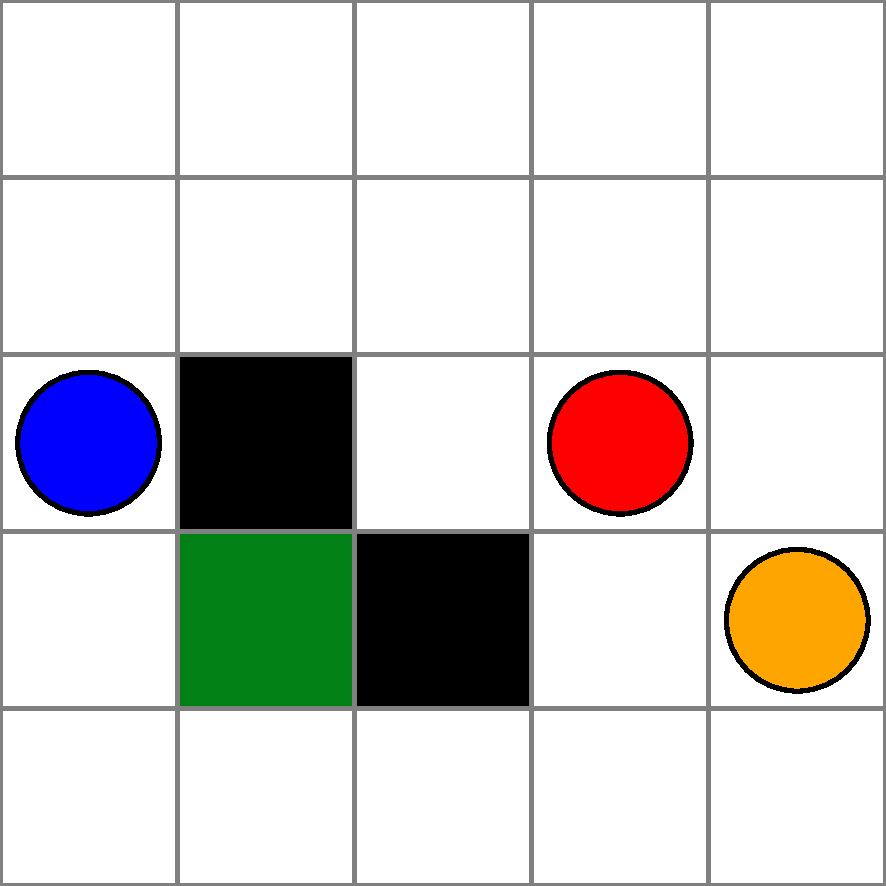
\includegraphics[width=\textwidth]{figures/scene_decomposition/g.pdf}
        \caption{Full problem.}
        \label{fig:ch6_fullg}
    \end{subfigure}
    \hfill
    \begin{subfigure}[b]{0.25\textwidth}
        \centering
        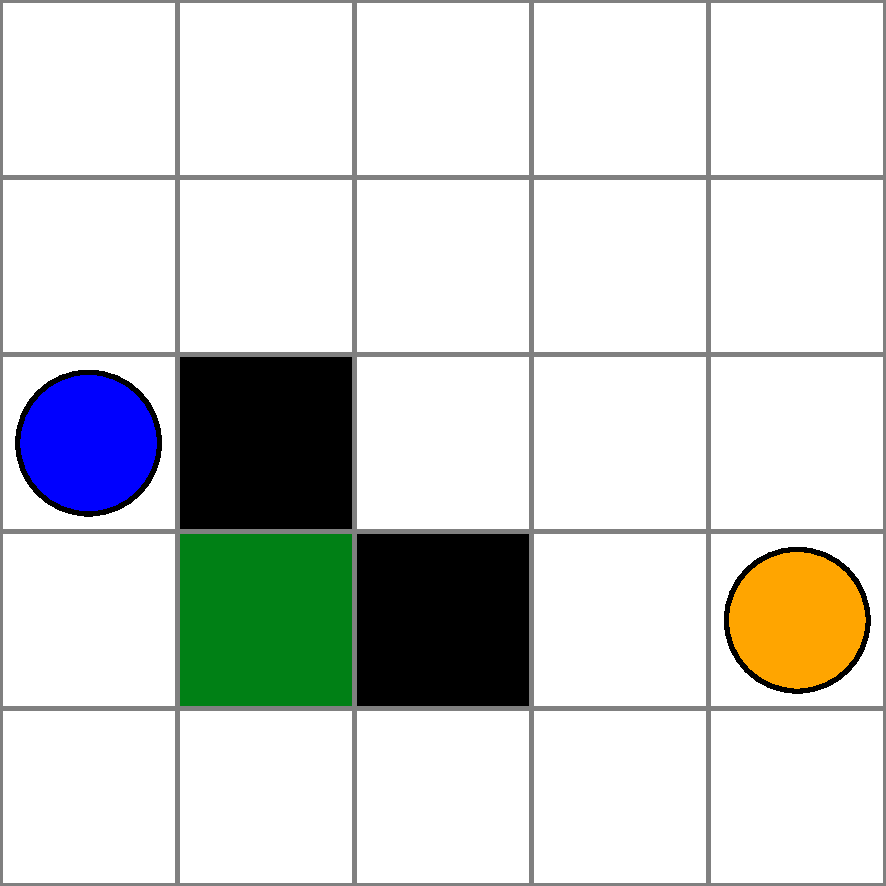
\includegraphics[width=\textwidth]{figures/scene_decomposition/g_sub1.pdf}
        \caption{Subproblem 1}
        \label{fig:ch6_subg1}
    \end{subfigure}
    \hfill
    \begin{subfigure}[b]{0.25\textwidth}
        \centering
        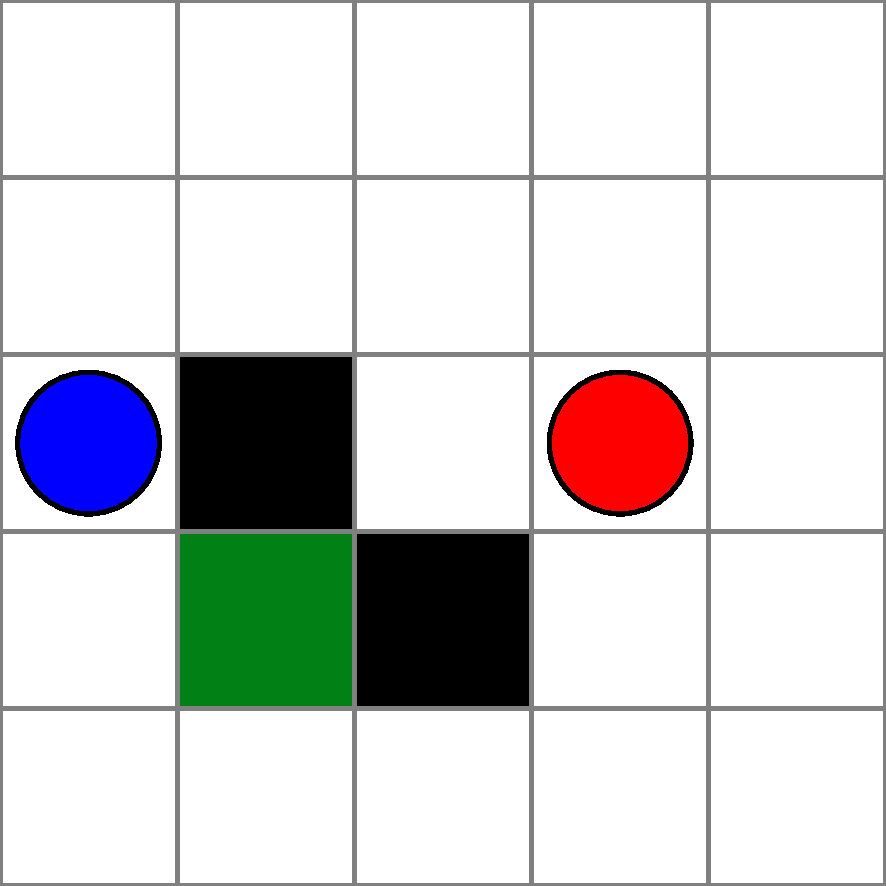
\includegraphics[width=\textwidth]{figures/scene_decomposition/g_sub2.pdf}
        \caption{Subproblem 2.}
        \label{fig:ch6_subg2}
    \end{subfigure}
    \caption{Example decomposition of the gridworld with two adversaries.}
    \label{fig:adv_gridworld_decomp}
\end{figure*}

\section{Decomposition and Fusion}
In this section we describe the process of problem decomposition and identify situations where subproblems are identical. We then introduce the attend, adapt, and transfer algorithm that automatically learns how to combine the subproblem solutions while learning a correction factor. 

\subsection{Problem Decomposition}
The goal of state-space decomposition is to identify a set of subspaces that each represent a similar, but smaller, version of the full problem. We denote the state space of the $i$th subproblem $S^{(i)}$ and the disturbance space $X^{(i)}$. The state $s^{(i)} \in S^{(i)}$ contains the components of $s$ that are associate with the $i$th subproblem and similarly for the disturbance $x^{(i)}$. A crucial constraint on the choice of decomposition is the ability to simulate transitions of the subproblems
\begin{equation}
    s_{t+1}^{(i)} \sim P( s^{(i)} \mid s_t^{(i)}, x_t^{(i)} ) \text{.}
\end{equation}

In the gridworld example, if we choose a decomposition where the state space consists only of the horizontal component of each agent, it is not clear how we would choose a transition model that is faithful to the original problem. Instead, if we choose a decomposition where the state space is the position of the ego and one adversary, and the disturbance space is the disturbance space of that adversary then we have reduced the problem a single-adversary gridworld which we know how to simulate. Indeed, in multi-agent problems a natural decomposition usually consists of the state spaces from a subset of of the agents. 

In 

\subsection{Solution Fusion}

\begin{equation}
\hat{Q}(s) = w_0(s) \hat{Q}_{\rm base}(s) + \sum_{i=1}^k w_i(s) g_x^{(i)}(\hat{Q}_i(g_s^{(i)}(s)))
\end{equation}

\begin{figure}[!t]
\centering
% TikZ diagram for black-box safety validation problem formulation.
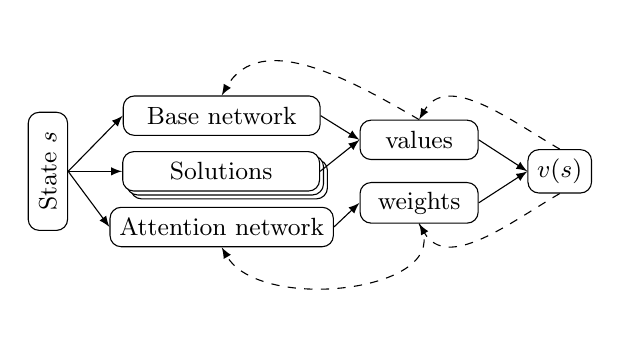
\begin{tikzpicture}
    \tikzstyle{every node}=[font=\small, align=center]
    \tikzset{
        n/.style={draw, rounded corners, minimum height=0.5cm, minimum width = 1.5cm},
        n2/.style={n, minimum width=2.5cm}
        }
    
    %state 
    \node (state) [n, rotate=90] {\small State $s$};
    
    %base network
    \node (base) [n2, above right of=state, xshift=1.5cm] {Base network};
    
    %Solutions
    \node (solutionsback1) [n2, right of=state, xshift=1.3cm, yshift=-0.1cm] {};
    \node (solutionsback2) [n2, fill=white, right of=state, xshift=1.25cm, yshift=-0.05cm] {};
    \node (solutions) [n2, fill=white, right of=state, xshift=1.2cm] {Solutions};
    
    %weights
    \node (attn) [n2, below right of=state, xshift=1.5cm] {Attention network};
    

    \node (values) [n, below right of=base, xshift=1.8cm, yshift = 0.4cm] {values};
    
     \node (weights) [n, above right of=attn, xshift=1.8cm, yshift = -0.4cm] {weights};
     
     \node (pfail) [n, minimum width = 0.5cm, right of=state, xshift=5.5cm] {$v(s)$};
    

    \draw[-latex] (state.south) -- (base.west);
    \draw[-latex] (state.south) -- (solutions.west);
    \draw[-latex] (state.south) -- (attn.west);
    
    \draw[-latex] (base.east) -- (values.west);
    \draw[-latex] (solutions.east) -- (values.west);
    \draw[-latex] (attn.east) -- (weights.west);
    
    \draw[-latex] (weights.east) -- (pfail.west);
    \draw[-latex] (values.east) -- (pfail.west);
    
    
    % backprop
    
    \draw [dashed, -latex] (weights.south) to [out=-1500,in=-60] (attn.south);
    \draw [dashed, -latex] (pfail.south) to [out=-150,in=-60] (weights.south);
    \draw [dashed, -latex] (values.north) to [out=150,in=60] (base.north);
    \draw [dashed, -latex] (pfail.north) to [out=150,in=60] (values.north);
\end{tikzpicture}
\caption{The A2T network. }
\label{fig:A2T_Network}
\vskip -0.5cm
\end{figure}



\section{Experiments}

\section{Adversarial Gridworld Example}

\begin{figure}
        \centering
        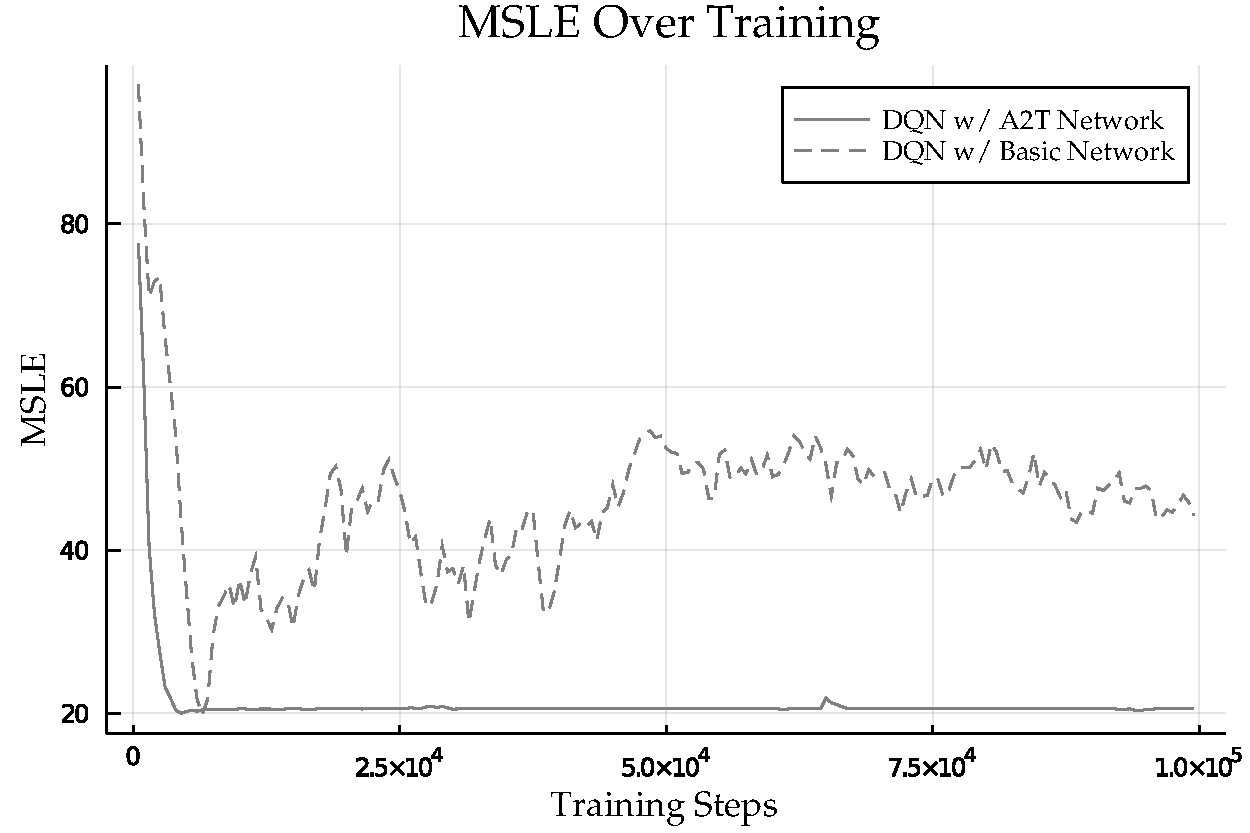
\includegraphics[width=\textwidth]{figures/scene_decomposition/training_comparison.pdf}
        \caption{Training comparison between A2T and basic network.}
        \label{fig:ch5_adv_gridworld_training}
\end{figure}


\section{T-Intersection Scenario}

\begin{table}
    \centering
    \caption{5-car Results}
    \label{tab:ch6_5car_results}
    \begin{tabular}{@{}lll@{}} 
        \toprule
        \textbf{Method} & \textbf{Failure Rate} & \textbf{Log Likelihood}\\
        \midrule
        Monte Carlo & \num{0.0} \pm \num{0.0} &  - \\
        Uniform Actions & \num{0.031} \pm \num{0.005} & \num{-173.01} \pm \num{42.925} \\
        Cross Entropy Method & \num{0.035} \pm \num{0.006} & \num{-82.672} \pm \num{7.342} \\
        DQN + A2T & \num{0.081} \pm \num{0.009} & \num{-19.938} \pm \num{7.317} \\
        \bottomrule
    \end{tabular}
\end{table}

\begin{figure}
        \centering
        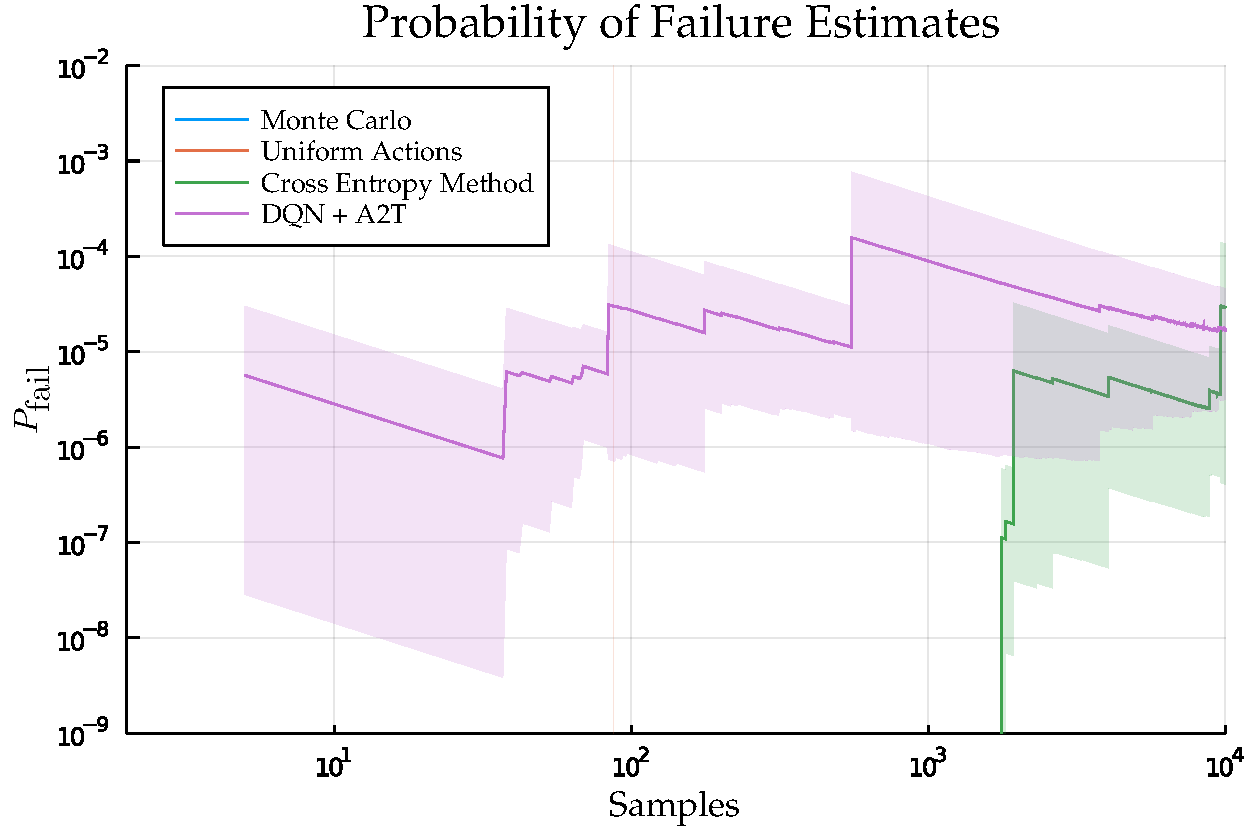
\includegraphics[width=\textwidth]{figures/scene_decomposition/pfail_5car.pdf}
        \caption{Comparison of techniques for $P_{\rm fail}$ estimation for the 5-car T-intersection scenario.}
        \label{fig:ch5_5car_pfail_estimation}
\end{figure}

\begin{figure}
    \centering
   \begin{subfigure}[t]{0.7\textwidth}
        \centering
        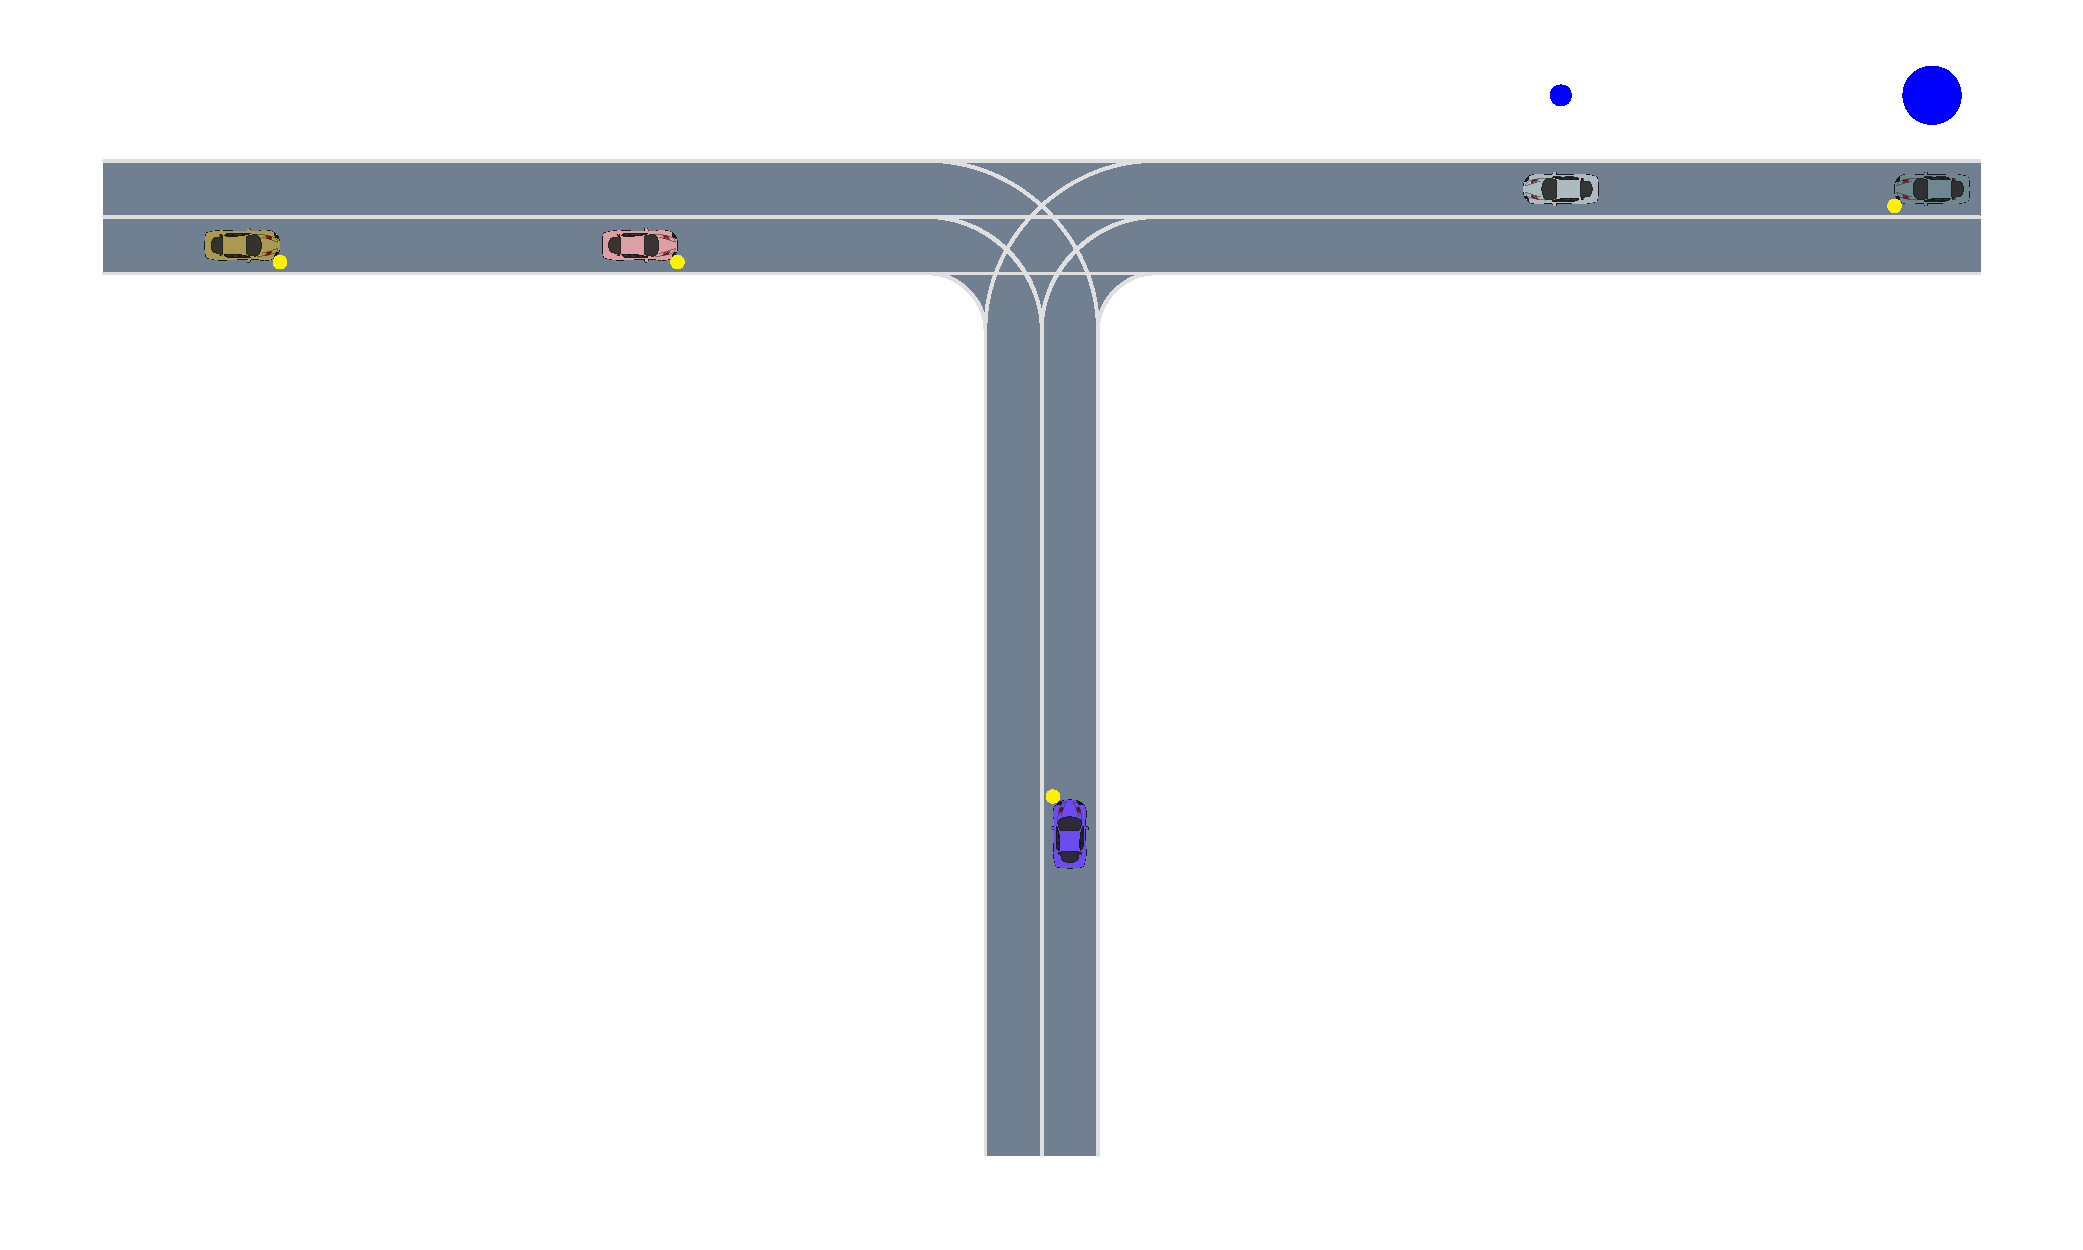
\includegraphics[width=\textwidth, trim={2cm 5cm 1cm 0},clip]{figures/scene_decomposition/f1_1.pdf}
    \end{subfigure}
    \begin{subfigure}[t]{0.7\textwidth}
        \centering
        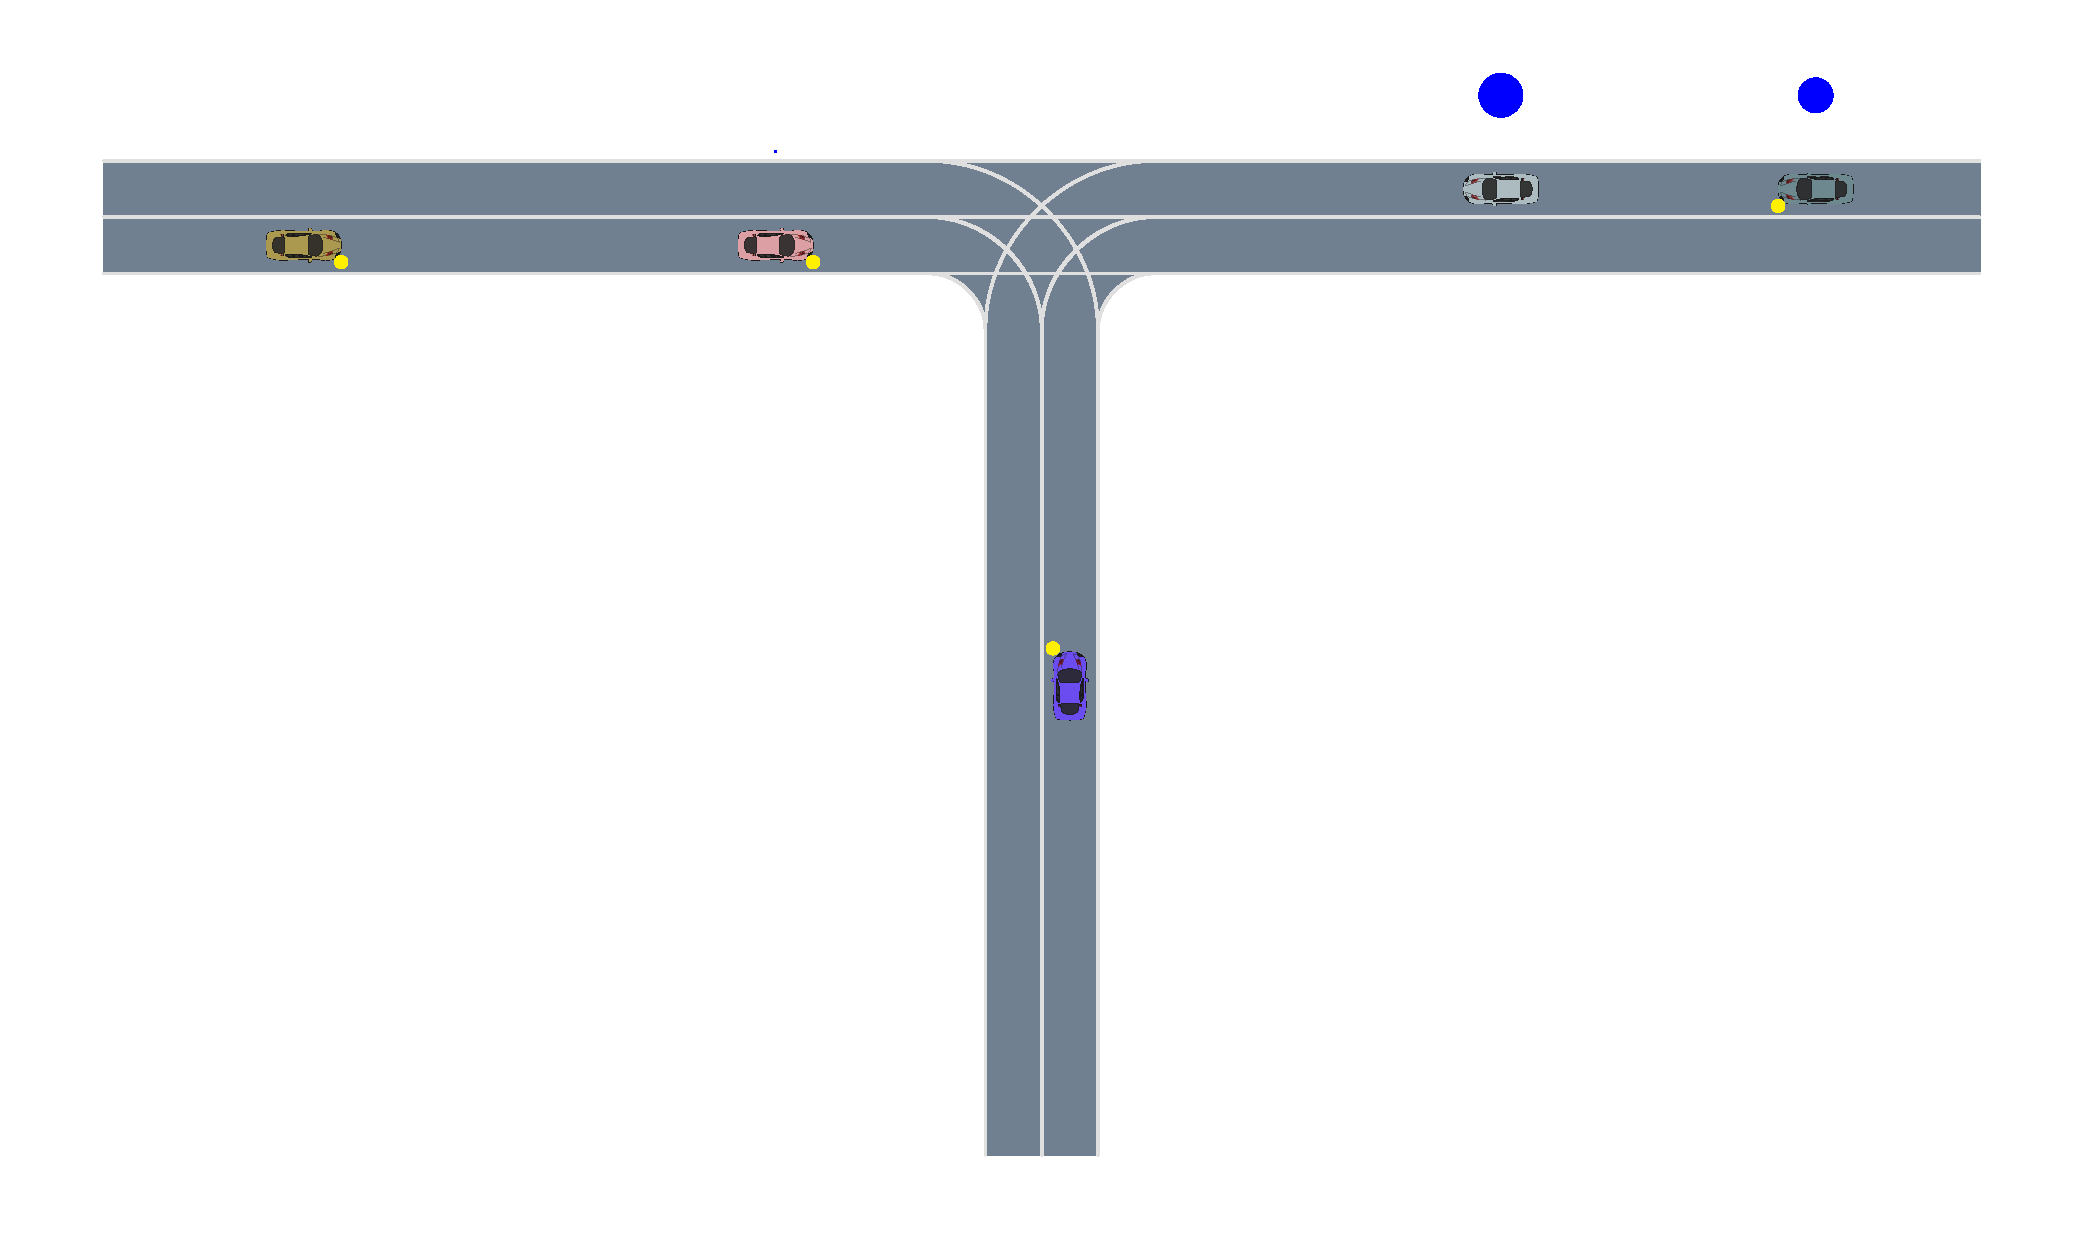
\includegraphics[width=\textwidth, trim={2cm 5cm 1cm 0},clip]{figures/scene_decomposition/f1_4.pdf}
    \end{subfigure}
    \begin{subfigure}[t]{0.7\textwidth}
    \centering
    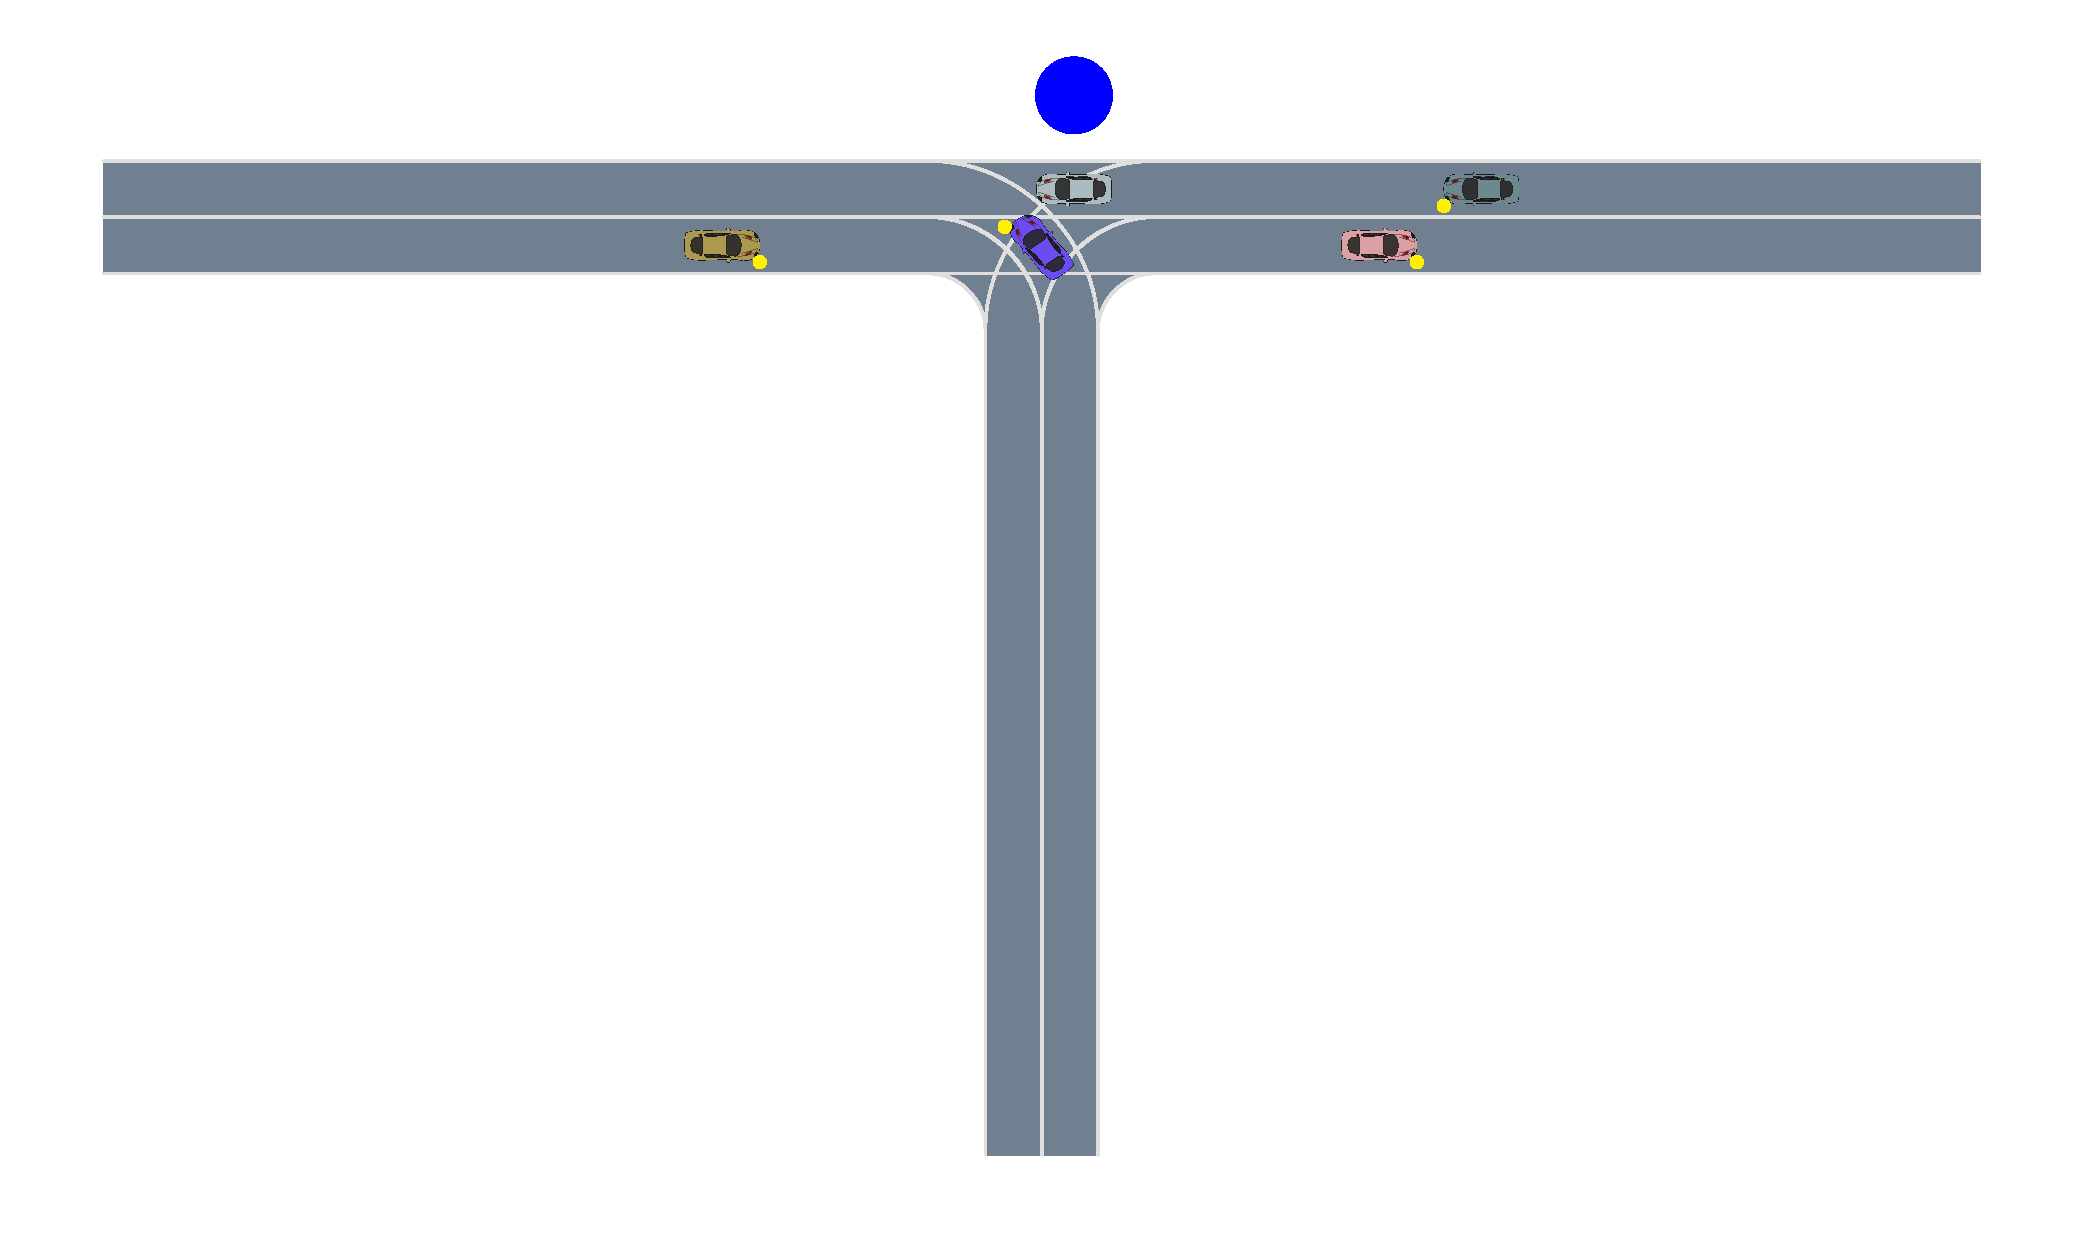
\includegraphics[width=\textwidth, trim={2cm 5cm 1cm 0},clip]{figures/scene_decomposition/f1_18.pdf}
\end{subfigure}
    \caption{Collision in 5-car scenario at timesteps $t=[1,4,18]$}
    \label{fig:two_car_collision}
    \vspace{-0.2in}
\end{figure}


\begin{figure}
    \centering
   \begin{subfigure}[t]{0.7\textwidth}
        \centering
        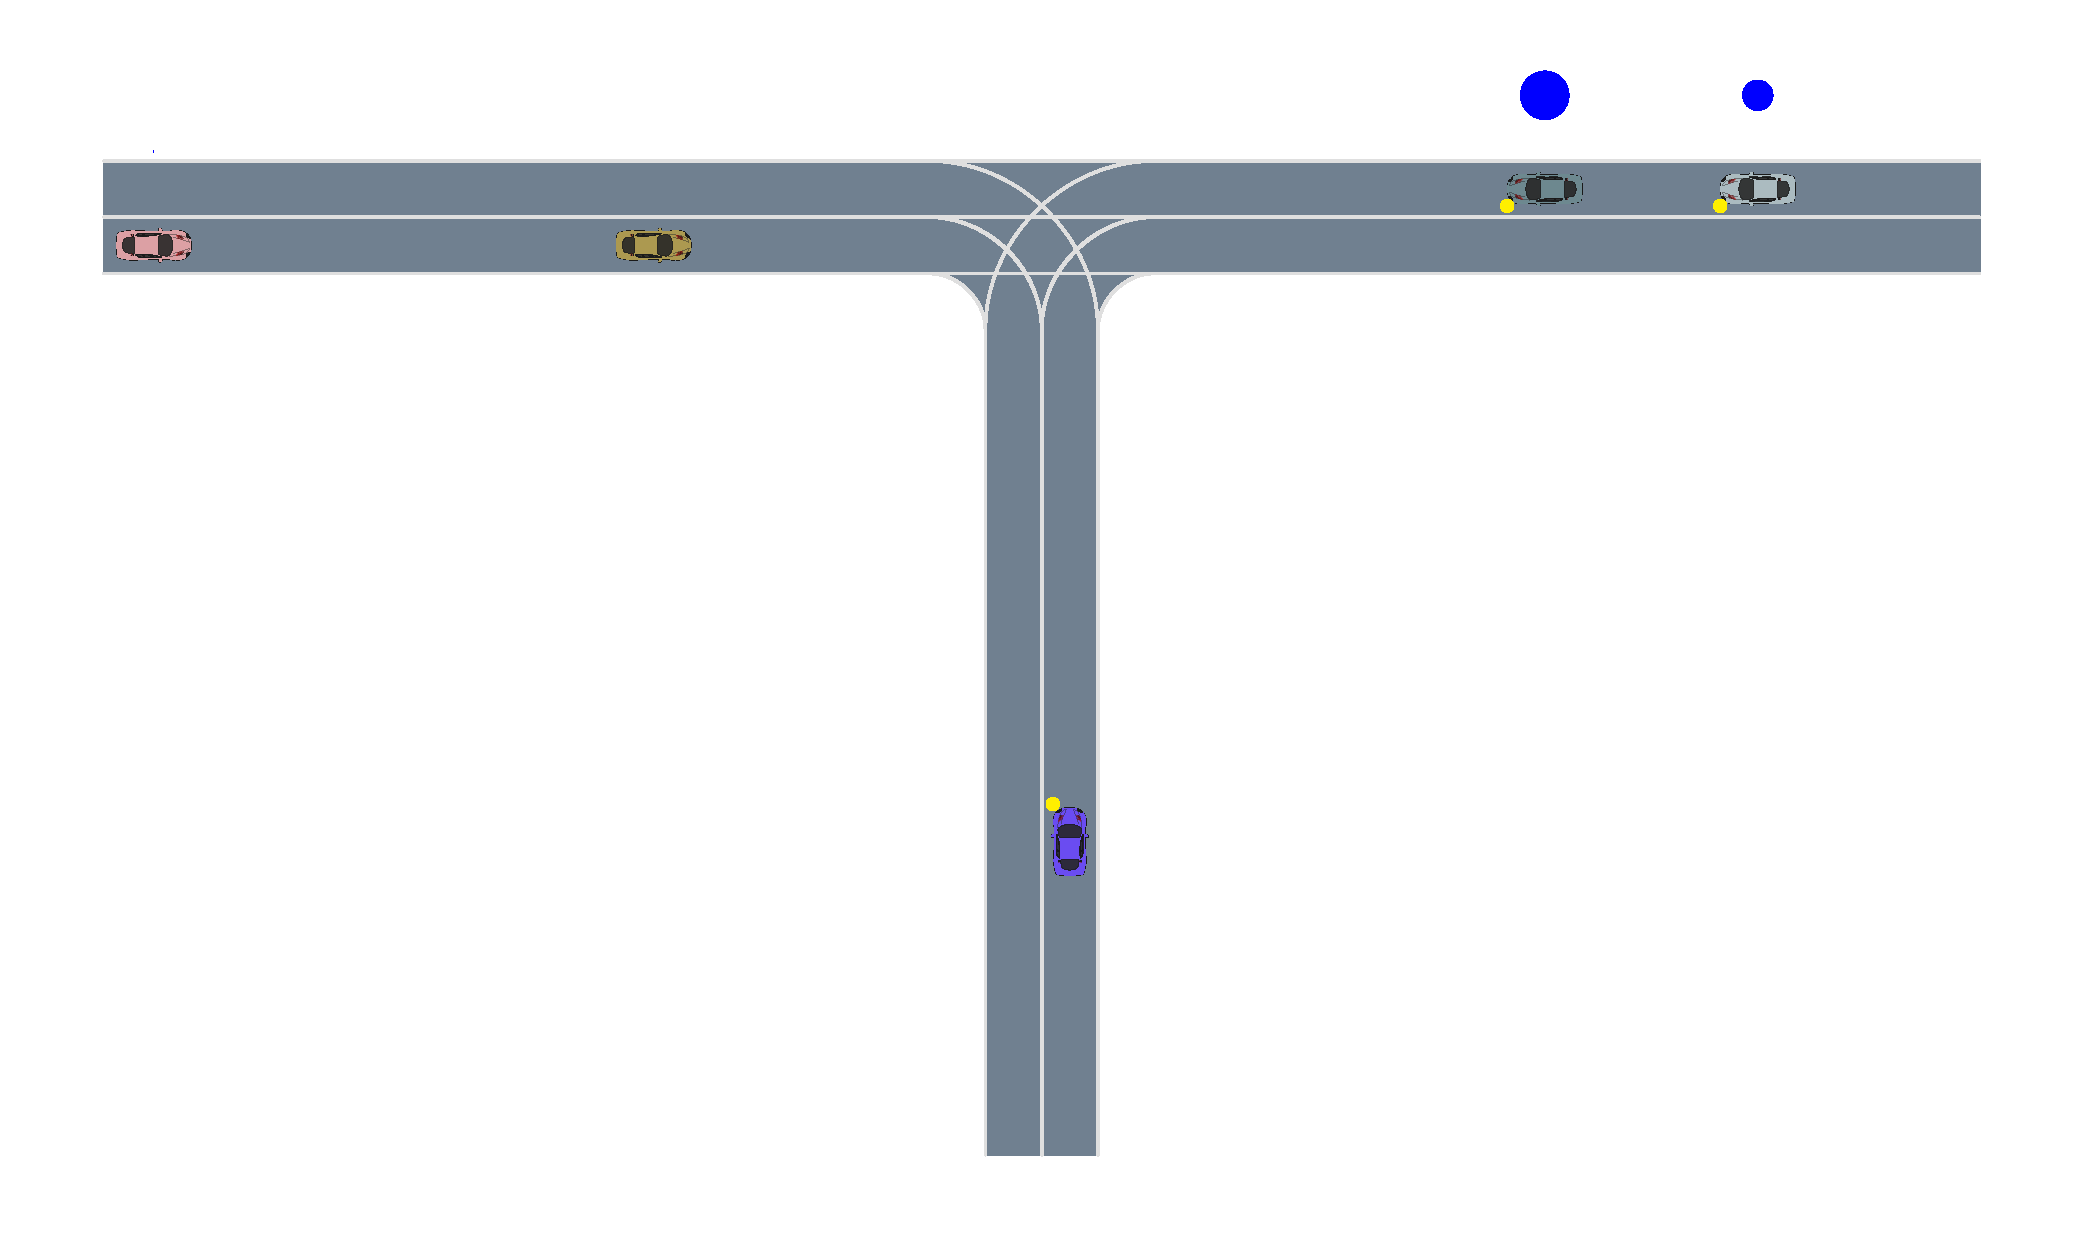
\includegraphics[width=\textwidth, trim={2cm 5cm 1cm 0},clip]{figures/scene_decomposition/f2_1.pdf}
    \end{subfigure}
    \begin{subfigure}[t]{0.7\textwidth}
        \centering
        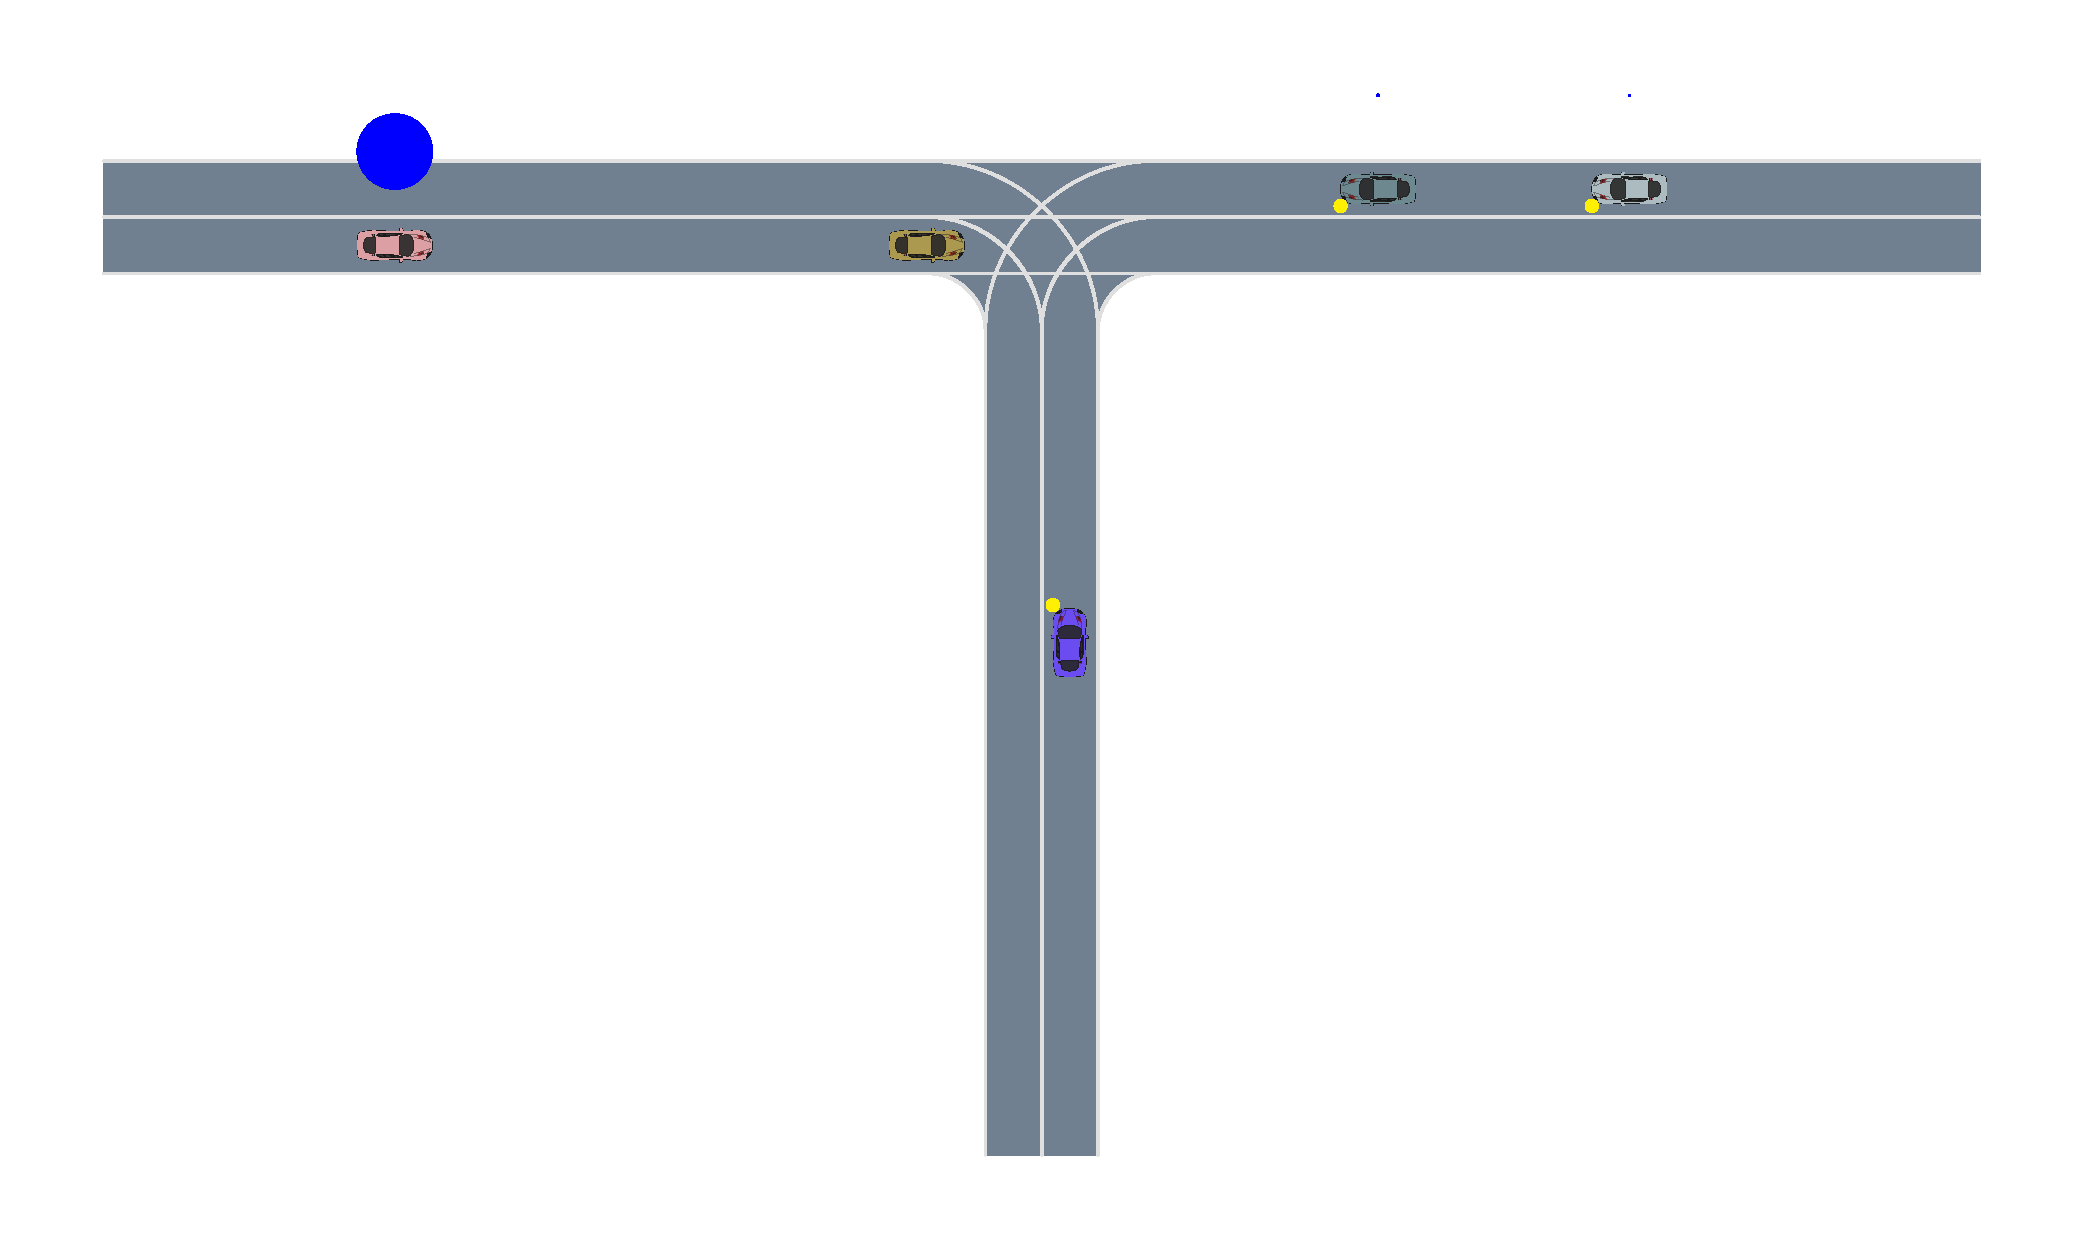
\includegraphics[width=\textwidth, trim={2cm 5cm 1cm 0},clip]{figures/scene_decomposition/f2_8.pdf}
    \end{subfigure}
    \begin{subfigure}[t]{0.7\textwidth}
    \centering
    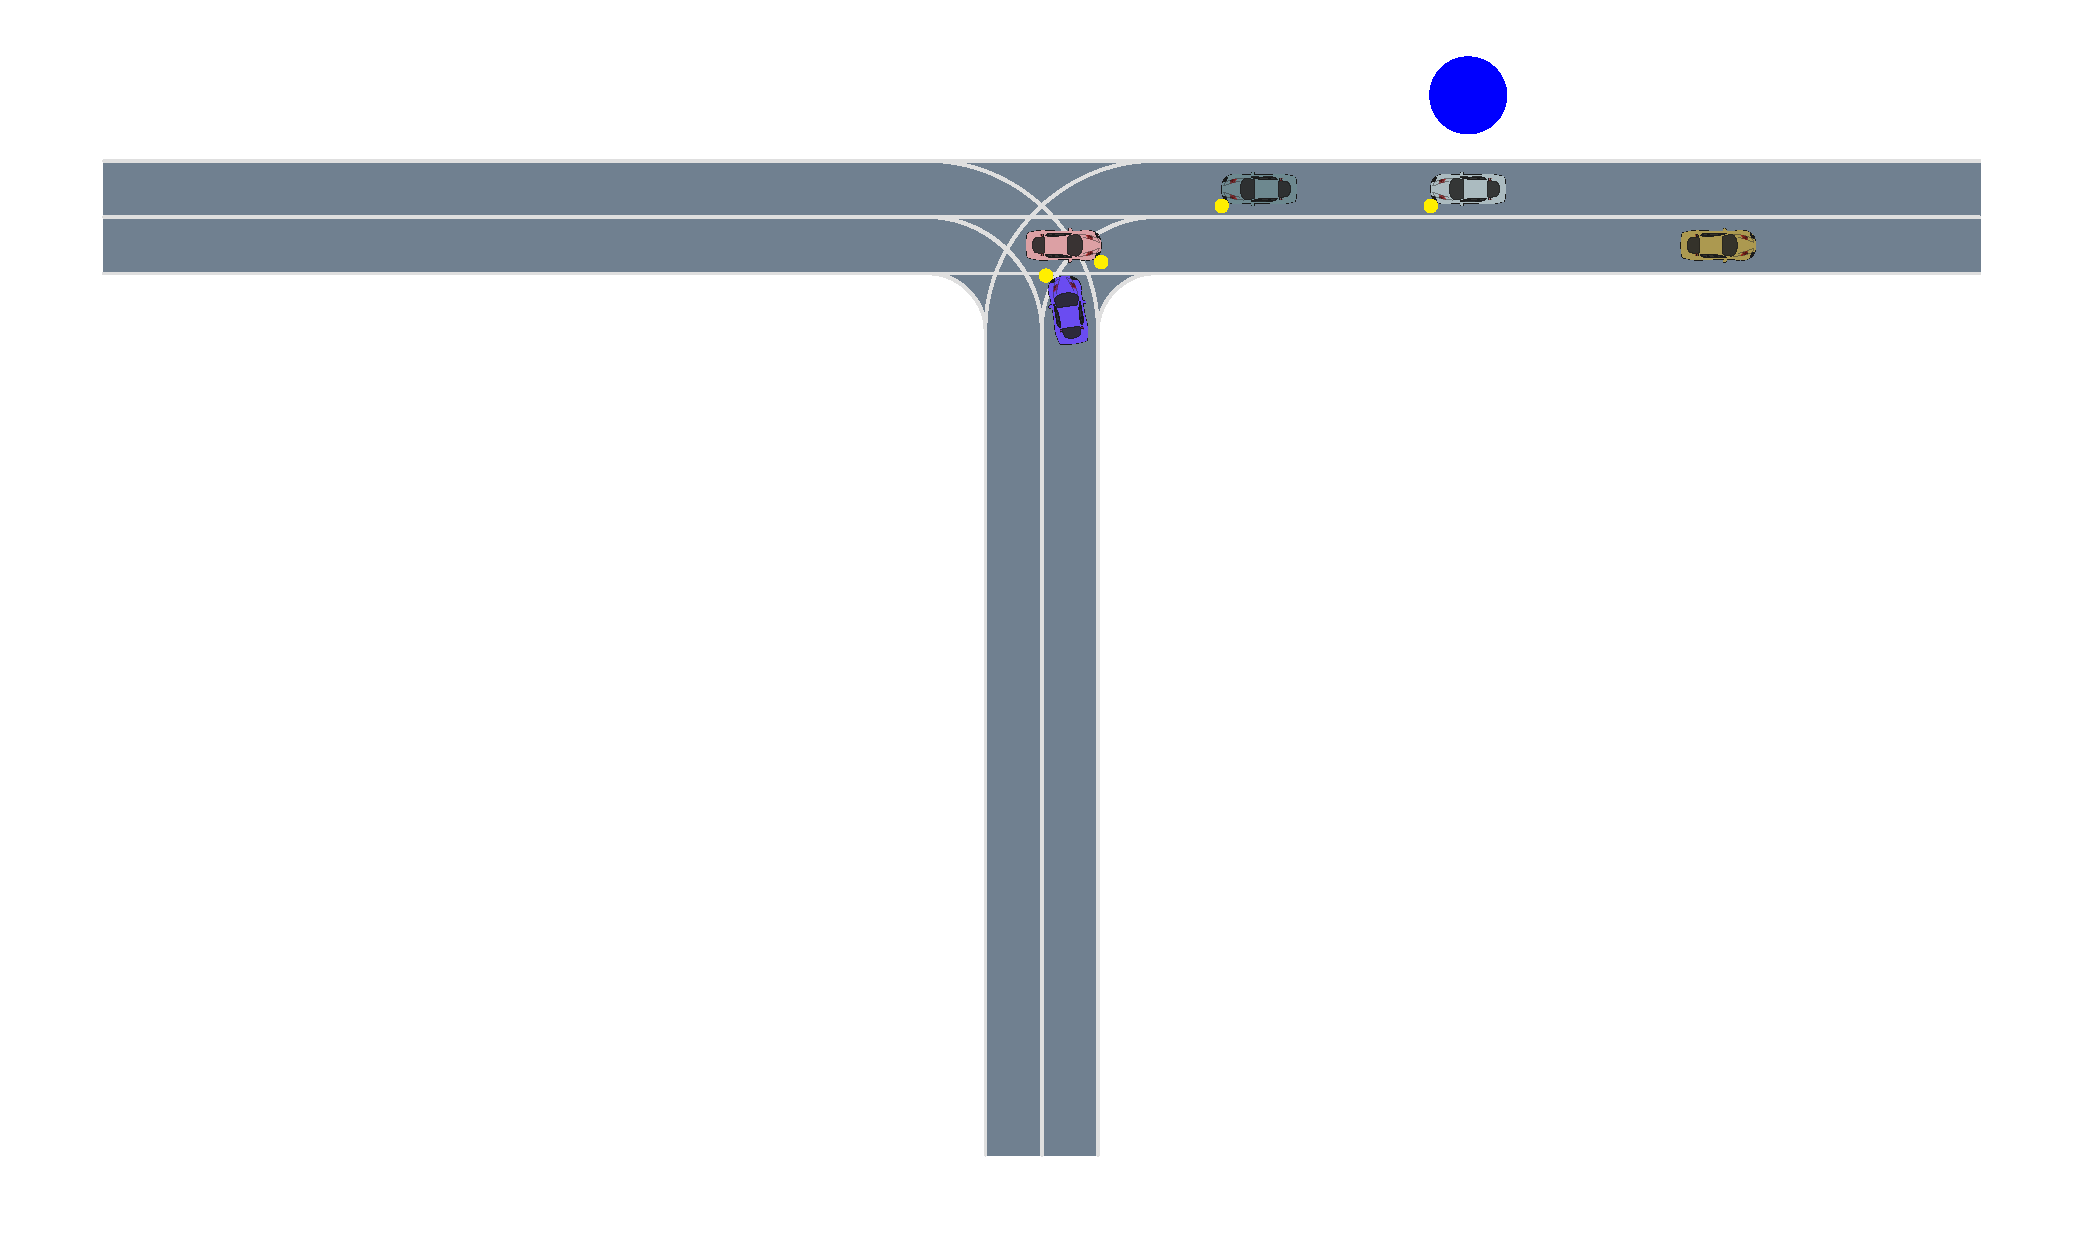
\includegraphics[width=\textwidth, trim={2cm 5cm 1cm 0},clip]{figures/scene_decomposition/f2_27.pdf}
\end{subfigure}
    \caption{Collision in 5-car scenario at timesteps $t=[1,8,27]$}
    \label{fig:two_car_collision}
    \vspace{-0.2in}
\end{figure}


\section{Discussion}

\chapter{Efficient Iterative Safety Validation}
In this chapter we consider the problem of validating many related systems sequentially. Most safety validation algorithms must start from scratch each time the system under test changes, but we demonstrate performance and efficiency benefits to sharing knowledge between safety validation tasks. We apply transfer learning algorithms to share knowledge between related tasks and perform experiments using the gridworld with adversary and crosswalk scenarios.

\section{Motivation}
Designing and certifying safety-critical systems generally involves assessing a sequence of closely related systems. Safety validation of complex systems often requires significant computational effort and existing approaches generally start from scratch each time the system under test is changed. The need to frequently perform safety validation on related systems therefore imposes a large computational burden, but also an opportunity to improve safety validation efficiency. 

% What we did
To improve the efficiency of safety validation across related systems, we use knowledge from the validation of previous systems to inform the validation of the next system. We formulate iterative safety validation as a transfer learning problem by modeling each safety validation task as a Markov decision process. The previously solved safety validation problems are used as the set of source tasks, and we transfer knowledge to future tasks in the form of action value functions. We use a set of state-dependent attention weights to automatically learn which previous solutions are applicable to the current problem.

We propose a new variation of the attend, adapt, and transfer (A2T) algorithm~\cite{rajendran2017attend} that transforms the state and action value spaces for each source task to increase knowledge transfer between dissimilar tasks and compare it to basic A2T and a fine-tuning baseline. We evaluate the initial performance, the final performance, and the number of training steps required to reach the same performance as a no-transfer algorithm. We consider four iterative safety validation tasks in gridworld and autonomous driving scenarios and demonstrate that transfer learning has the potential to significantly improve the performance and sample efficiency of safety validation algorithms.


\section{Transfer Learning}
% What is transfer learning for RL?
Transfer learning is concerned with using knowledge gained by solving one task to improve the learning process in another related task~\cite{taylor2009transfer}. In reinforcement learning, each task is an MDP and each solution is a policy. When tasks have different state and action spaces, we require task mappings that relate the states and actions between tasks. Task mappings may be provided by a human~\cite{taylor2007transfer} or learned from data~\cite{taylor2008autonomous}. If the state and action spaces are the same, then tasks can share a variety of low-level information such as experience samples $(s, a, s', r)$, action value functions, policies, or models of the environment. High-level information, such as a set of options, shaping rewards or feature encodings, may also be transferred to improve learning on a new task. One challenge in transfer learning is \emph{negative transfer} where knowledge from one or more source tasks impairs the performance on the current task. Negative transfer can be mitigated using an attention mechanism, or a human oracle that decides which tasks are relevant~\cite{taylor2009transfer}. 

% How are transfer learning algorithms evaluated
Transfer learning algorithms can be evaluated against a no-transfer alternative in a variety of ways (\cref{fig:transfer_metrics}). \emph{Jumpstart} is the amount of improvement before any training has occurred, \emph{final performance} is the difference between the best performances achieved, \emph{total reward} is the area under the training curve,  and \emph{steps to threshold} is the difference between the number of training steps required to reach a specified threshold.

\begin{figure}
\centering
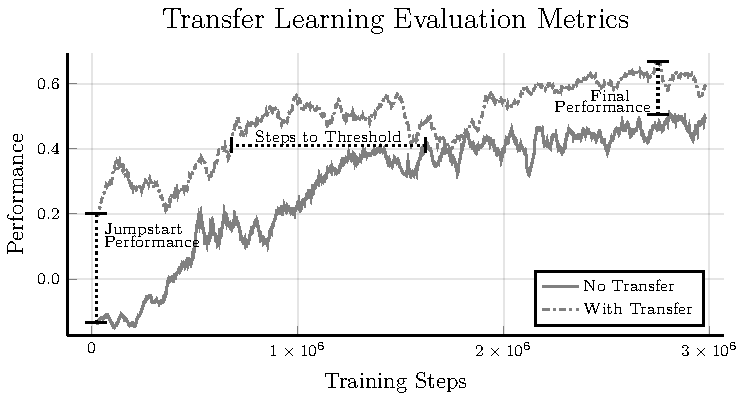
\includegraphics[width=0.8\linewidth]{figures/iterative_validation/transfer_metrics}
\caption{Metrics for evaluating transfer learning algorithms. }
\label{fig:transfer_metrics}
\end{figure}

% How is safety validation a transfer learning problem
Safety validation MDPs may differ in a variety of ways, which we can explain using an example based on autonomous driving. If validation is performed on two different road geometries (e.g. highway-driving  and an intersection), then the state space and disturbance space may be different. If we fix the road geometry, then the transition model may vary if we validate different driving policies. The reward function will vary if the disturbance model changes or we alter the set of failure states. In this work, we consider systems with different behavior operating in similar environments. We, therefore, assume that the state space, disturbance space, and reward function remain fixed while the transition model varies between tasks.

\section{Proposed Approach}
This section describes our approach for improving iterative safety validation using transfer learning. We first show how to formulate iterative safety validation as a sequence of tasks and specify two ways that knowledge transfer may occur. We then introduce A2T as our choice of transfer learning algorithm and propose a modification to it.

\subsection{Problem Formulation}
Suppose we are performing safety validation on a sequence of related systems and  must validate each system before observing the next one. We model this problem as solving a sequence of MDPs (or tasks) $[T_1, T_2, \ldots]$ where the $i$th task is given by $T_i = (\mathcal{S}, \mathcal{X}, P_i, R, \gamma)$. Due to variations in system behavior, the transition model $P_i$ is unique to each task, while $\mathcal{S}$, $\mathcal{X}$, $R$, and $\gamma$ are shared across tasks. We wish to develop a learning algorithm $L$ that solves task $i$ given the $i-1$ previous solutions $[K_1, K_2, \ldots, K_{i-1}]$ such that
\begin{equation}
    K_i = L(T_i; K_{1:i-1}) \text{.}
\end{equation}
The previous solutions may take the form of value functions or policies. The learning procedure is iterative because the new solution $K_i$ can be added to the set of previous solutions when solving the next task $T_{i+1}$. Since all previous solutions are used, $L$ must avoid negative transfer by learning which source task solutions are applicable to the current task.



In the context of safety validation, we hypothesize two qualitatively distinct ways that the tasks will be related. The first case is that of a \emph{learning system} which is improving its performance from task to task. Each task is therefore more challenging for the adversary since failures that were present in previous tasks may no longer exist or may only occur due to a narrower range of disturbances. In this context, the most recent solutions are likely to provide the most relevant information and large parts of those solutions may be directly applicable to the new task. The second case is that of \emph{comparable systems} where the systems have a similar level of competency but exhibit different behavior. Disturbance trajectories that lead to failure for one system may not cause failure in any other systems, although they might share similar conceptual failure modes. In this setting, direct transfer of solutions may be ineffective, and we need to rely on other types of knowledge. 


\subsection{Choice of Learning Algorithm}
\begin{figure}
\centering
\resizebox{0.7\columnwidth}{!}{% TikZ diagram for black-box safety validation problem formulation.
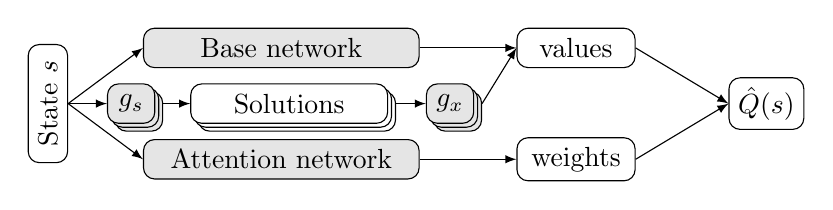
\begin{tikzpicture}
    \tikzstyle{every node}=[font=\normalsize, align=center]
    \tikzset{
        n/.style={draw, rounded corners, minimum height=0.5cm, minimum width = 1.5cm},
        n2/.style={n, minimum width=3.5cm},
        n4/.style={n, minimum width=2.5cm},
        n3/.style={n, minimum width=0.6cm}
        }
    
    %state 
    \node (state) [n, rotate=90] { State $s$};
    
    %base network
    \node (base) [n2, fill=black!10, above right of=state, anchor=west, xshift=0.5cm] {Base network};
    
     %State Transforms
    \node (stback1) [n3, fill=black!10, right of=state, anchor=west, xshift=-0.15cm, yshift=-0.1cm] {};
    \node (stback2) [n3, fill=black!10, right of=state, anchor=west, xshift=-0.2cm, yshift=-0.05cm] {};
    \node (st) [n3, fill=black!10, right of=state, anchor=west, xshift = -0.25cm] {$g_s$};
    
    %Solutions
    \node (solutionsback1) [n4, right of=st, xshift=-.15cm, yshift=-0.1cm, anchor=west] {};
    \node (solutionsback2) [n4, fill=white, right of=st, xshift=-0.2cm, yshift=-0.05cm, anchor=west] {};
    \node (solutions) [n4, fill=white, right of=st, anchor=west, xshift = -0.25cm] {Solutions};
    
    %Action Transforms
    \node (atback1) [n3, fill=black!10, right of=solutions, anchor=east, xshift=1.45cm, yshift=-0.1cm] {};
    \node (atback2) [n3, fill=black!10, right of=solutions, anchor=east, xshift=1.4cm, yshift=-0.05cm] {};
    \node (at) [n3, fill=black!10, right of=solutions, anchor=east, xshift=1.35cm] {$g_x$};
    
    %weights
    \node (attn) [n2, fill=black!10, below right of=state, anchor=west, xshift=0.5cm] {Attention network};
    

    \node (values) [n, right of=base, anchor=east, xshift=3.5cm] {values};
    
     \node (weights) [n, right of=attn, anchor=east, xshift=3.5cm] {weights};
     
     \node (pfail) [n, minimum width = 0.5cm, right of=at, anchor=east, xshift=3.5cm] {$\hat{Q}(s)$};
    

    \draw[-latex] (state.south) -- (base.west);
    \draw[-latex] (state.south) -- (st.west);
    \draw[-latex] (st.east) + (0.1cm, 0cm) -- (solutions.west);
    \draw[-latex] (solutions.east) + (0.1cm, 0cm) -- (at.west);
    \draw[-latex] (state.south) -- (attn.west);
    
    \draw[-latex] (base.east) -- (values.west);
    \draw[-latex] (at.east) + (0.1cm, 0cm) -- (values.west);
    \draw[-latex] (attn.east) -- (weights.west);
    
    \draw[-latex] (weights.east) -- (pfail.west);
    \draw[-latex] (values.east) -- (pfail.west);
    
    
    % backprop
    
    % \draw [dashed, -latex] (weights.south) to [out=-1500,in=-60] (attn.south);
    % \draw [dashed, -latex] (pfail.south) to [out=-150,in=-60] (weights.south);
    % \draw [dashed, -latex] (values.north) to [out=150,in=60] (base.north);
    % \draw [dashed, -latex] (pfail.north) to [out=150,in=60] (values.north);
\end{tikzpicture}}
\caption{Architecture of A2T with state and action transformation.}
\label{fig:a2t_architecture}
\end{figure}

To accelerate safety validation we use the attend, adapt, and transfer (A2T) learning algorithm~\cite{rajendran2017attend} with a minor modification. A2T accelerates learning on a new task by combining the solutions of $k$ previous tasks using a learned set of state-dependent attention weights. To avoid negative transfer, A2T simultaneously learns a solution from scratch so there are a total of $k+1$ solutions and as  many attention weights. A2T can be used to estimate optimal policies or optimal value functions and we found it most straightforward to estimate the optimal action value function. When $Q^*$ is estimated by a neural network, called a $Q$-network, the input is a vector representing the state and the output is a vector representing the values of a discrete set of disturbances. To make this clear, if $\mathcal{X} \subseteq \mathbb{R}^m$, then $\hat{Q}(s) \in \mathbb{R}^m$, is a vector that represents the estimates of the optimal values for each disturbance. The action value function is estimated by the expression
\begin{equation}
\hat{Q}(s) = w_0(s) \hat{Q}_{\rm base}(s) + \sum_{i=1}^k w_i(s) \hat{Q}_i(s) \label{eq:A2T}
\end{equation}
where $\hat{Q}_i$ comes from the $i$th source task, $\hat{Q}_{\rm base}$ is learned from scratch and $w_i(s)$ is the $i$th attention weight, normalized so $\sum_{i=0}^m w_i(s) = 1$.


To handle substantially different system behaviors, we propose a modification of A2T where we include a learned transformation of the state and action value function for each of the $k$ previous solutions. If the state space $\mathcal{S} \subseteq \mathbb{R}^n$, then we define a \emph{state transformation} as a function $g_s : \mathbb{R}^n \to \mathbb{R}^n$ and an \emph{action value transformation} as a function $g_x : \mathbb{R}^m \to \mathbb{R}^m$. Applied to the A2T algorithm, the action value estimate with state and action space transformations is given by
\begin{equation}
\hat{Q}(s) = w_0(s) \hat{Q}_{\rm base}(s) + \sum_{i=1}^k w_i(s) g_x^{(i)}(\hat{Q}_i(g_s^{(i)}(s)))
\end{equation}
where $g_s^{(i)}$ and $g_x^{(i)}$ are the state and action value transformations for the $i$th source solution. 



The A2T algorithm with state and action value transformations can be encoded as the network architecture shown in \cref{fig:a2t_architecture}. The state is used as input to the base network, the source solutions, and the attention network. The base network is a $Q$-network that learns from scratch. The $k$ source solutions are the $Q$-networks that represent the optimal solutions of the source tasks. The source solutions are preceded by a state transformation and followed by an action value transformation. These transformations have the same output dimension as input dimension and are initialized to the identity transformation (with a small amount of noise for breaking symmetry). The attention network has $k+1$ output units with a softmax layer for normalization. The $Q$ values of each source solution and the base network are weighted by the corresponding attention weight and summed together to get a final estimate. The network is trained using the DQN algorithm, which updates the parameters in the base network, the attention network, and the state and action value transformations. If the source solutions are not differentiable with respect to the state (as in the case of a lookup table) then we would apply gradient free optimization~\cite{kochenderfer2019algorithms} to the state transformation.

\begin{figure}
    \centering
    \captionsetup[subfigure]{format=hang}
    \begin{subfigure}[t]{0.25\linewidth}
        \centering
        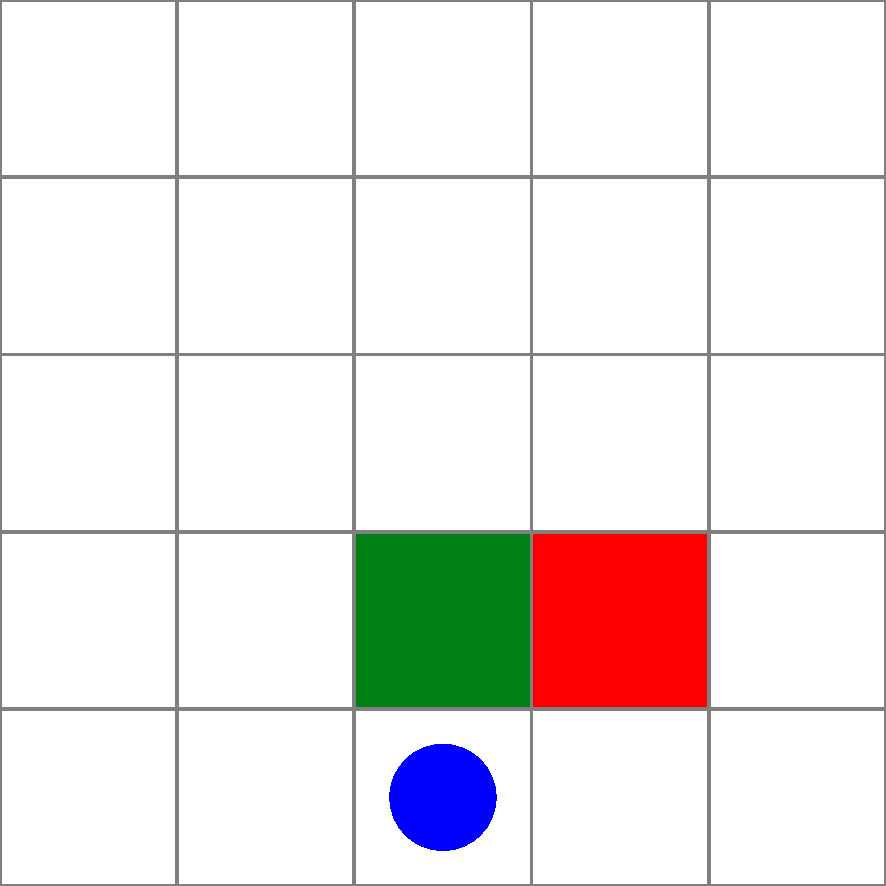
\includegraphics[width=\textwidth]{figures/iterative_validation/gridworld1.pdf}
        \caption{\scriptsize Source MDP}    
        \label{fig:motiation_source}
    \end{subfigure}
    \hfill
    \begin{subfigure}[t]{0.25\linewidth}  
        \centering 
        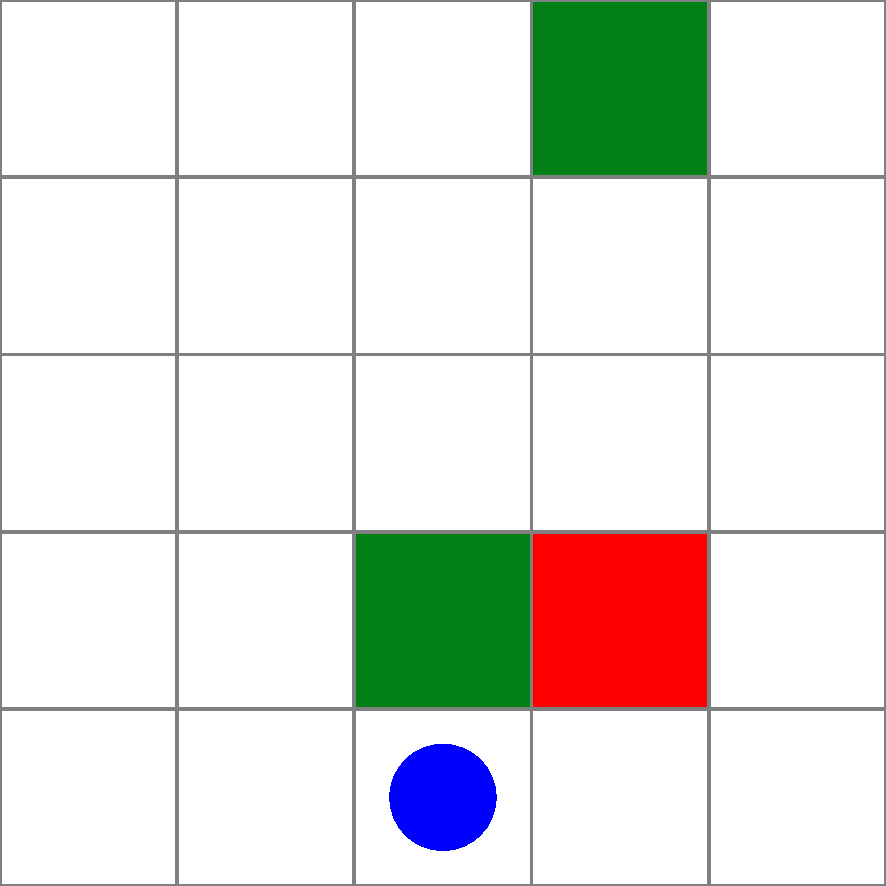
\includegraphics[width=\textwidth]{figures/iterative_validation/gridworld2.pdf}
        \caption{\scriptsize Locally similar}  
        \label{fig:motivation_a2t}
    \end{subfigure}
    \hfill
    \begin{subfigure}[t]{0.25\linewidth}   
        \centering 
        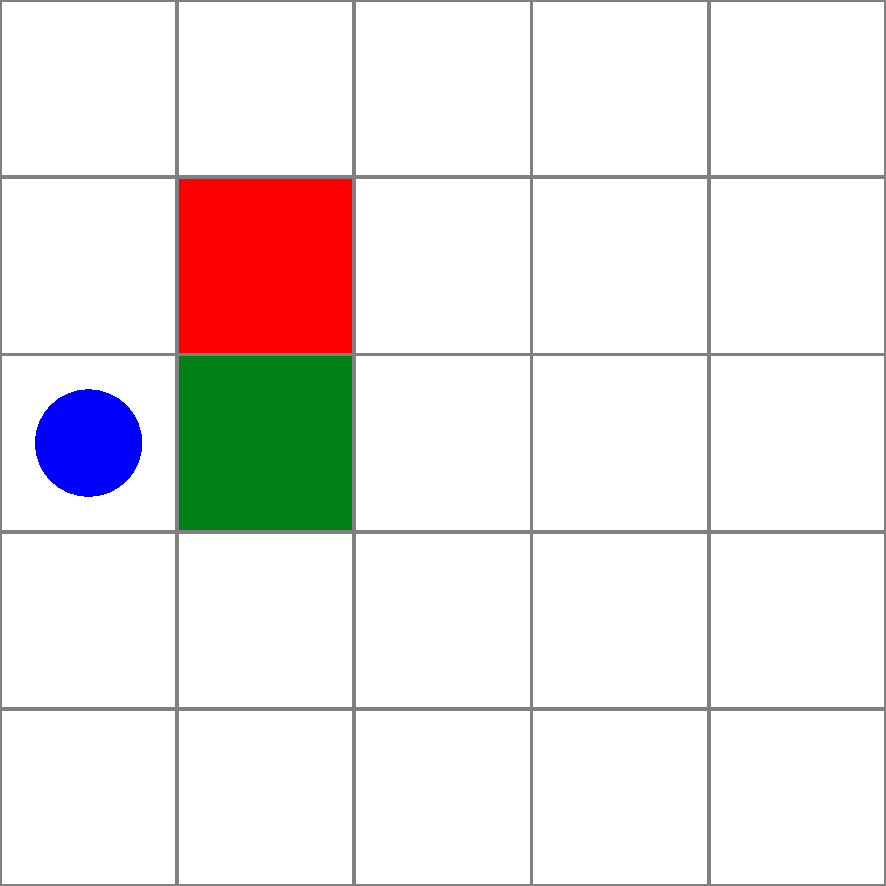
\includegraphics[width=\textwidth]{figures/iterative_validation/gridworld4.pdf}
        \caption{\scriptsize Transformed}
        \label{fig:motivation_sat}
    \end{subfigure}
    \caption{Knowledge transfer scenarios.}
    \label{fig:motivation}
\end{figure}

\paragraph{Motivation.} Here we provide some intuition for our choice of transfer learning algorithm and the reason for the state and action transformations. Suppose we are solving a sequence of tasks (\cref{fig:motivation}), each is a gridworld where an agent (blue circle) moves between adjacent squares attempting to achieve high reward (green squares) while avoiding states with low reward (red squares). Given the optimal action value function for a source MDP (\cref{fig:motiation_source}), we wish to transfer it to two related tasks. In the first transfer problem (\cref{fig:motivation_a2t}), the reward distribution is locally similar to the source MDP, and only differs in one state. In this case, a policy that works well in the source task will also work well in the new task, especially when the agent is in a state where the local reward landscape matches up (as depicted). A2T will work well in this setting because it can quickly learn attention weights that favor the source policy in most states, and only require our baseline solution when the agent is near the top right corner. In the second transfer problem (\cref{fig:motivation_sat}), A2T is likely to behave poorly because there are no states in which the source policy can be directly applied to achieve high reward. If, however, we could transform the state space by reflecting it across the diagonal and rotate the actions of the agent by \SI{90}{\degree}, then we could directly apply the source policy. This is the motivation for applying transformations both before and after the source solutions. 


\section{Experiments}

This section describes the iterative most likely failure analysis of the gridworld with an adversary and the crosswalk scenarios. We first describe how both scenarios are modified for iterative safety validation. Each scenario has two transfer learning problems, one for validating a learning system that improves over time, and the other for validating a set of comparable systems with different behaviors. We then describe the experimental setup and the results. 

% Gridworld with adversary

\subsection{Task Setup}

% Description of the difference between tasks
The first safety validation problem we consider is the gridworld scenario with a single adversary. We design two sets of tasks that correspond to the learning system and comparable systems settings. For the learning system, the ego agent is trained using DQN against an orange agent that behaves randomly. Over $\num{e6}$ training steps, \num{10} versions of the system policy were stored, each with an increasing level of performance. Each safety validation task has the adversary validate an increasingly capable version of the learning system. The performance of the optimal policy on each task is measured on every other task and plotted in \cref{fig:ch7_comps_lgw} to observe the default transfer between tasks. 

For the comparable systems setting, each task has a different distribution of reward locations, reward values and location of walls. The system learns an optimal policy using dynamic programming~\cite{dmubook}, assuming the adversary behaves randomly. Each system is therefore equally competent, but some configurations of the gridworld are more challenging than others. A similar comparison plot of the optimal policy for each tasks applied to all othere is shown in \cref{fig:ch7_comps_cgw}.

\begin{figure}
    \centering
    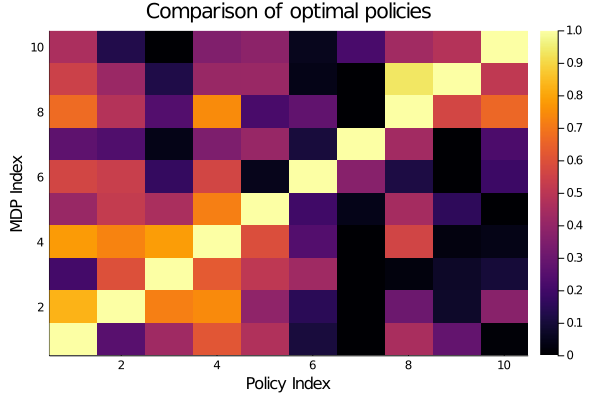
\includegraphics[width=0.7\textwidth]{figures/iterative_validation/gridworld_improving.png}
    \caption{Task and policy comparisons for a learning gridworld agent.}
    \label{fig:ch7_comps_lgw}
\end{figure}

\begin{figure}
    \centering
    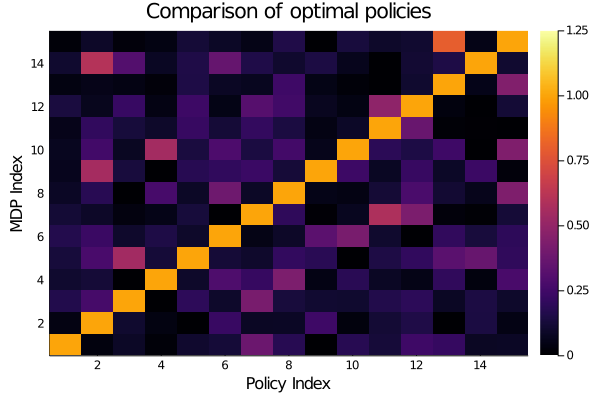
\includegraphics[width=0.7\textwidth]{figures/iterative_validation/moving_rewards_heatmap_bigbatch.png}
    \caption{Task and policy comparisons for comparable gridworld agents.}
    \label{fig:ch7_comps_cgw}
\end{figure}


\begin{figure}
\centering
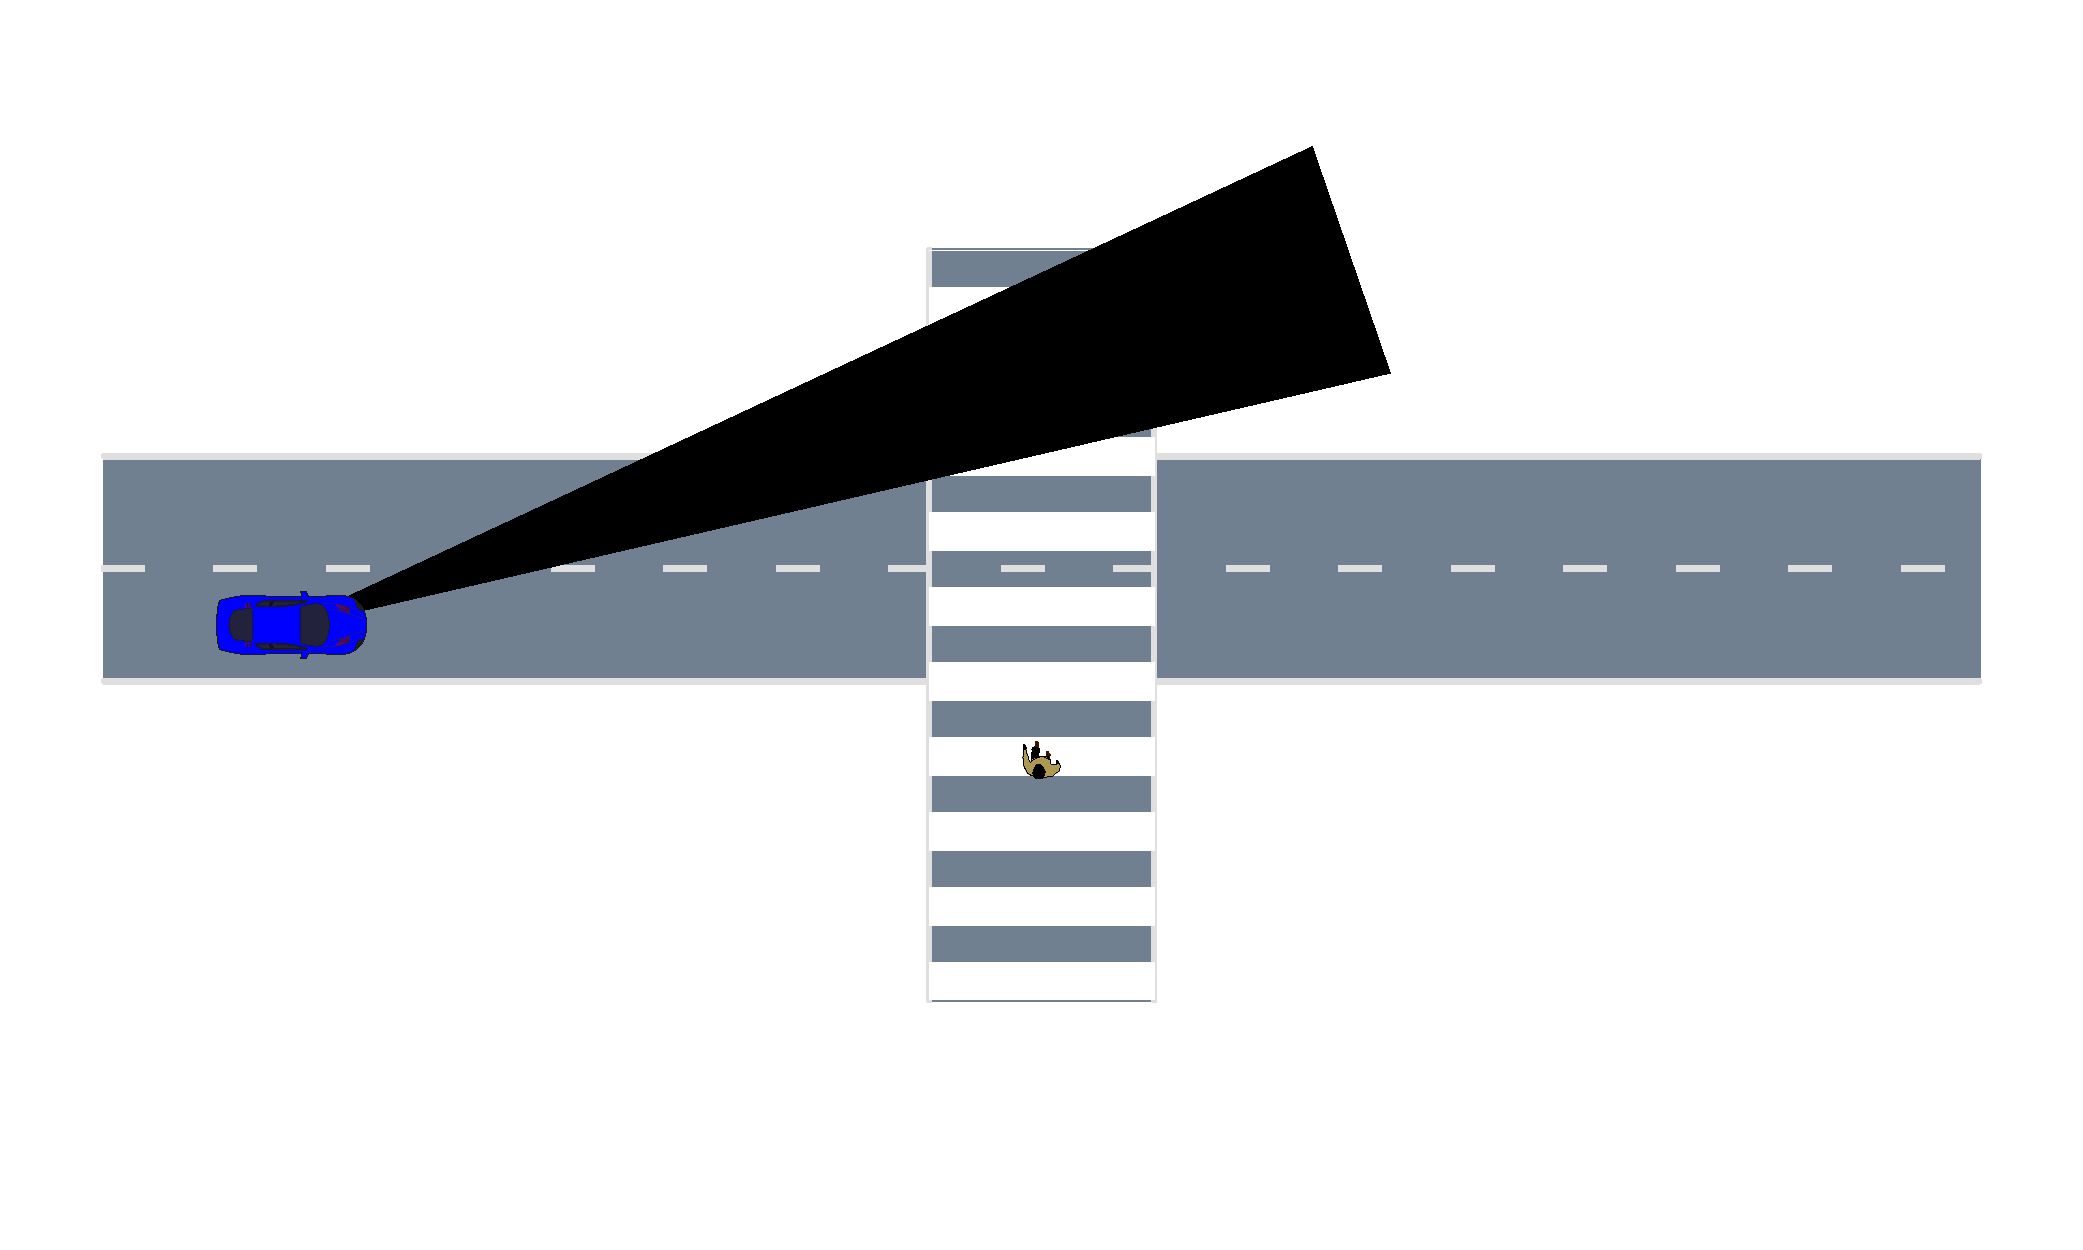
\includegraphics[trim={0 7cm 10cm 6.5cm},clip, width=0.7\linewidth]{figures/iterative_validation/blindspot.pdf}
\caption{Crosswalk scenario with AV blindpsot. }
\label{fig:av_blindspot}
\end{figure}

% Description of the MDP
The second safety validation problem we model is a modified version of the crosswalk scenario where the vehicle has a blindspot as shown in \cref{fig:av_blindspot}. We design two sets of tasks corresponding to a learning system setting and a comparable systems setting. Since the autonomous vehicle does not use machine learning, we simulate an improvement by progressively shrinking the blind spot of the vehicle. The blind spot remains in the same direction (\SI{20}{\degree} from the horizontal), but reduces in width from \SI{30}{\degree} to \SI{6}{\degree} over \num{10} iterations. The vehicle therefore has a decreasing rate of failures over the tasks but there is some overlap in failure modes between adjacent tasks (see \cref{fig:ch7_comps_lad} for comparison of tasks and optimal policies). For the comparable systems setting, each system has a blind spot sampled uniformly at random with a direction in the range $[\SI{-30}{\degree}, \SI{30}{\degree}]$ and an angular width in the range $[\SI{3}{\degree}, \SI{9}{\degree}]$. From a population of \num{30} tasks, we selected \num{9} tasks that differed substantially, to make the transfer problem as challenging as possible within our setting. Two tasks differed if the optimal safety validation policy of one performs poorly on the other. We show the comparison of taks performance in \cref{fig:ch7_comps_cad}

\begin{figure}
    \centering
    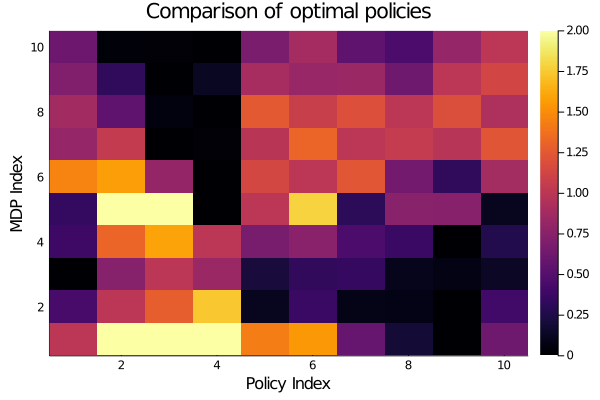
\includegraphics[width=0.7\textwidth]{figures/iterative_validation/blindspot_improving_heatmap.png}
    \caption{Task and policy comparisons for a learning autonomous driving agent.}
    \label{fig:ch7_comps_lad}
\end{figure}

\begin{figure}
    \centering
    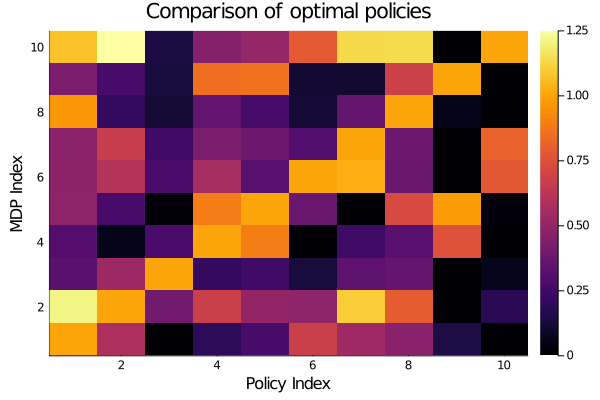
\includegraphics[width=0.7\textwidth]{figures/iterative_validation/blindspot_heatmap_bigbatch.png}
    \caption{Task and policy comparisons for comparable autonomous driving agents.}
    \label{fig:ch7_comps_cad}
\end{figure}


\subsection{Experimental Setup}

The experimental procedure is as follows. For each task in a set of tasks, we solve for an optimal $Q$-network from scratch using DQN with prioritized replay, double $Q$-learning~\cite{Hasselt2016deep}, and the Huber loss. We construct a learning curve during training by periodically storing the evaluation of the $Q$-network. For the second task onward, we then solve it using the same learning algorithm with the following $Q$-network  architectures:
\begin{itemize}
    \item \textbf{Fine-tune}: Train the last layer of the previous $Q$-network.
    \item \textbf{A2T}: A2T architecture with previous $Q$-networks as the source solutions.
    \item \textbf{A2T+SAVT}:  A2T architecture augmented with linear state and action value transformations.
\end{itemize}
The networks are initialized with Xavier initialization~\cite{glorot2010understanding}, while the transformations were initialized to the identity matrix with uniform random noise  in the range [-\num{1e-3}, \num{1e-3}] added to the parameters to break symmetry. Additional information on network architecture and hyperparameters is shown in \cref{tab:hyperparameters}.


\begin{table}
    \centering
    \caption{Network architectures and hyperparameters. }
    \label{tab:hyperparameters}
    \begin{tabular}{@{}ll@{}} 
        \toprule
        \textbf{Parameter} & \textbf{Value}  \\
        \midrule
        Base network & 3 hidden layers, [\num{64}, \num{32}, \num{16}] units\\
        Attention network & 1 hidden layer, \num{16} units \\
        Activation function & relu \\
        State/Action transform & Linear \\
        Training steps & \num{3e6} \\
        Batch size & \num{64} \\
        Learning rate $\alpha$ & \num{4e-5} (GW), \num{5e-5} (AD) \\
        Target update frequency & \num{2000} (GW), \num{3000} (AD) \\
        Evaluation frequency & \num{2000} \\
        No. evaluation episodes  & \num{300} \\
        Exploration policy & $\epsilon$-greedy with $\epsilon \in [1, 0.1]$\\
        \bottomrule
    \end{tabular}
\end{table}

% Processing the learning curves
We filter each learning curve using a moving-average filter with a width of \num{20} evaluations steps to help remove the noise due to finite sample evaluation and any outlier evaluation points. For each learning curve we identify the \emph{near-optimal} performance as $\mu - \sigma$, where $\mu$ and $\sigma$ are the mean and standard deviation of the performance in a window with a width of \num{100} evaluation steps around the point of maximum performance. We use near-optimal performance because it is a more stable measure of how fast the learning took place than the point of maximum performance.

% computing evaluation metrics
The jumpstart is the difference in initial performance between a transfer and no-transfer learning algorithms. It can be computed from the first entries in the learning curves. When reporting jumpstart, we only include fine-tuning and A2T because A2T+SAVT has the same outputs as A2T until the transformations deviate from identity. The final performance is the difference in near-optimal performance between the transfer and no-transfer learning algorithms. The steps to threshold metric measures how many training steps are required for a transfer learning algorithm to reach the near-optimal performance of the no-transfer algorithm.

% normalization of metrics. 
The metrics are normalized with reference to the learning curve of the no-transfer algorithm because the initial and near-optimal performance varies between tasks. Let $y$ be the performance (initial or final) of a transfer learning algorithm and $y_{\rm ref}$ be the performance of the no-transfer learning algorithm, then we report the fractional difference in performance $(y - y_{\rm ref})/|y_{\rm ref}|$. Let $t$ be the number of training steps required to reach a threshold for a transfer learning algorithm and $t_{\rm ref}$ be the same quantity for the no-transfer learning algorithm, then we report the ratio $t / t_{\rm ref}$.

% Notes
We use the number of training steps rather than the wall clock time because we assume that the cost of running the simulator is much larger than the cost of updating the parameters of the model. This is a good assumption for high-fidelity simulators that are often used for validating safety-critical systems. We also assume that the training time of previous source tasks is a sunk cost and it is not included in our efficiency metric. This assumption is valid in the case of iterative safety validation because the new version of the system must be validated regardless of the approach used. When using A2T in a real-world setting, we would not solve each task from scratch and therefore the source solutions would take the form of A2T networks. A practitioner may wish to compress the A2T network~\cite{julian2019deep} into a traditional architecture before it is used as a source solution. We chose to use the networks trained from scratch for ease of implementation and to isolate the effects of transfer learning from other issues.


\subsection{Results}
\begin{figure*}
    \centering
    \begin{subfigure}[b]{0.32\textwidth}
        \centering
        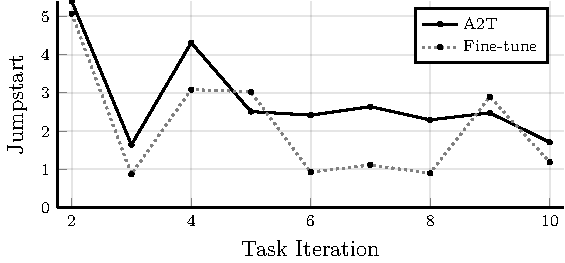
\includegraphics[width=\textwidth]{figures/iterative_validation/gridworld_learning/jumpstart.pdf}
        \caption{Jumpstart fractional improvement.}
        \label{fig:gwl_jumpstart}
    \end{subfigure}
    \hfill
    \begin{subfigure}[b]{0.32\textwidth}
        \centering
        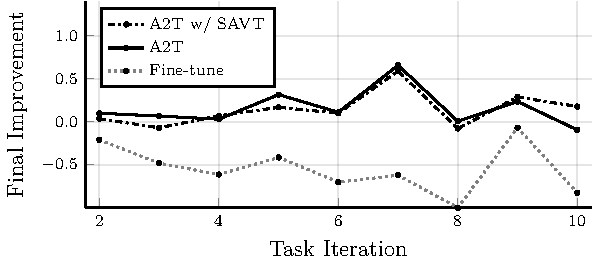
\includegraphics[width=\textwidth]{figures/iterative_validation/gridworld_learning/peak_performance.pdf}
        \caption{Final fractional improvement.}
        \label{fig:gwl_final}
    \end{subfigure}
    \hfill
    \begin{subfigure}[b]{0.32\textwidth}
        \centering
        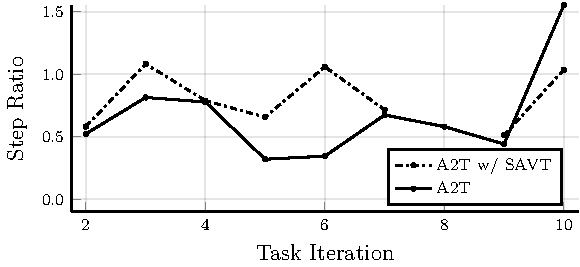
\includegraphics[width=\textwidth]{figures/iterative_validation/gridworld_learning/steps_to_threshold.pdf}
        \caption{Step ratio to threshold.}
        \label{fig:gwl_step}
    \end{subfigure}
    \caption{Evaluation metrics for the gridworld scenario with a learning system.}
    \label{fig:gwl}
\end{figure*}



\begin{figure*}
    \centering
    \begin{subfigure}[b]{0.32\textwidth}
        \centering
        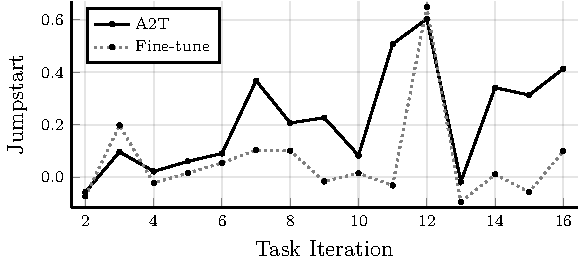
\includegraphics[width=\textwidth]{figures/iterative_validation/gridworld_comparison/jumpstart.pdf}
        \caption{Jumpstart fractional improvement.}
        \label{fig:gwc_jumpstart}
    \end{subfigure}
    \hfill
    \begin{subfigure}[b]{0.32\textwidth}
        \centering
        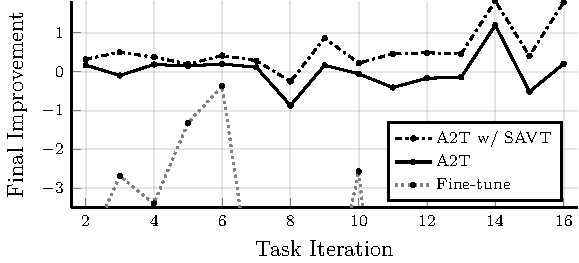
\includegraphics[width=\textwidth]{figures/iterative_validation/gridworld_comparison/peak_performance.pdf}
        \caption{Final fractional improvement.}
        \label{fig:gwc_final}
    \end{subfigure}
    \hfill
    \begin{subfigure}[b]{0.32\textwidth}
        \centering
        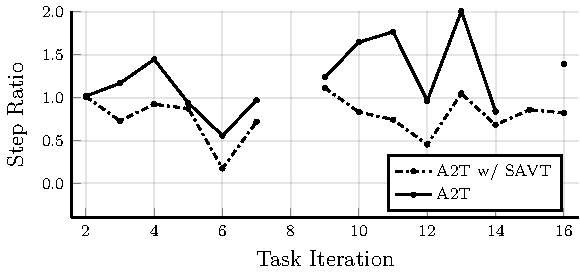
\includegraphics[width=\textwidth]{figures/iterative_validation/gridworld_comparison/steps_to_threshold.pdf}
        \caption{Step ratio to threshold.}
        \label{fig:gwc_step}
    \end{subfigure}
    \caption{Evaluation metrics for the gridworld scenario with comparable systems.}
    \label{fig:gwc}
\end{figure*}




\begin{figure*}
    \centering
    \begin{subfigure}[b]{0.32\textwidth}
        \centering
        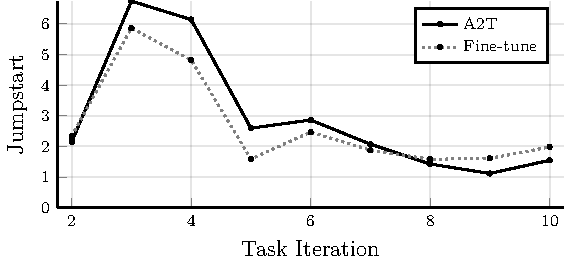
\includegraphics[width=\textwidth]{figures/iterative_validation/driving_learning/jumpstart.pdf}
        \caption{Jumpstart fractional improvement.}
        \label{fig:adl_jumpstart}
    \end{subfigure}
    \hfill
    \begin{subfigure}[b]{0.32\textwidth}
        \centering
        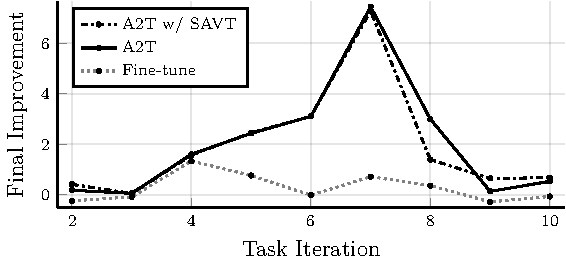
\includegraphics[width=\textwidth]{figures/iterative_validation/driving_learning/peak_performance.pdf}
        \caption{Final fractional improvement.}
        \label{fig:adl_final}
    \end{subfigure}
    \hfill
    \begin{subfigure}[b]{0.32\textwidth}
        \centering
        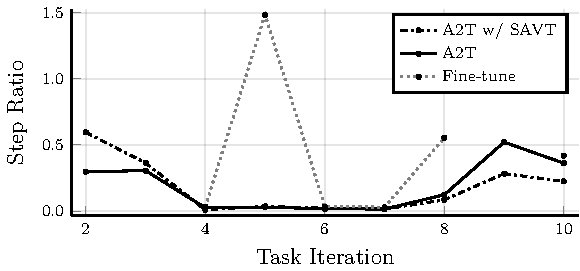
\includegraphics[width=\textwidth]{figures/iterative_validation/driving_learning/steps_to_threshold.pdf}
        \caption{Step ratio to threshold.}
        \label{fig:adl_step}
    \end{subfigure}
    \caption{Evaluation metrics for the autonomous driving scenario with a learning system.}
    \label{fig:adl}
\end{figure*}




\begin{figure*}
    \centering
    \begin{subfigure}[b]{0.32\textwidth}
        \centering
        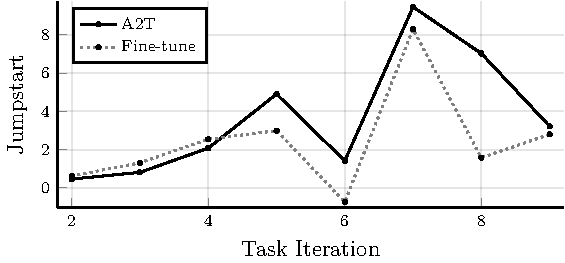
\includegraphics[width=\textwidth]{figures/iterative_validation/driving_comparison/jumpstart.pdf}
        \caption{Jumpstart fractional improvement.}
        \label{fig:adc_jumpstart}
    \end{subfigure}
    \hfill
    \begin{subfigure}[b]{0.32\textwidth}
        \centering
        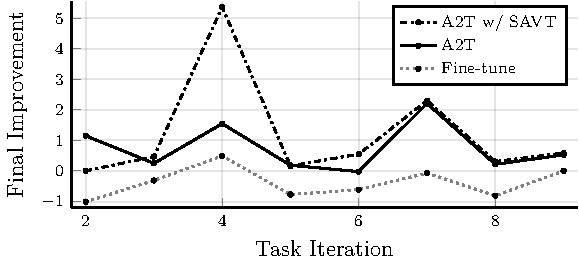
\includegraphics[width=\textwidth]{figures/iterative_validation/driving_comparison/peak_performance.pdf}
        \caption{Final fractional improvement.}
        \label{fig:adc_final}
    \end{subfigure}
    \hfill
    \begin{subfigure}[b]{0.32\textwidth}
        \centering
        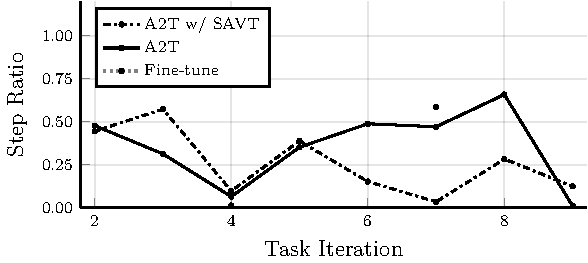
\includegraphics[width=\textwidth]{figures/iterative_validation/driving_comparison/steps_to_threshold.pdf}
        \caption{Step ratio to threshold.}
        \label{fig:adc_step}
    \end{subfigure}
    \caption{Evaluation metrics for the autonomous driving scenario with a comparable systems.}
    \label{fig:adc}
\end{figure*}


We solved each of the four safety validation tasks using 3 transfer learning algorithms and report the evaluation metrics against the task index in \cref{fig:gwl,fig:gwc,fig:adl,fig:adc}. The discussion of the results is grouped by evaluation metric. 


\paragraph{Jumpstart.}
\Cref{fig:gwl_jumpstart,fig:gwc_jumpstart,fig:adl_jumpstart,fig:adc_jumpstart} show the jumpstart of the fine-tune and A2T architectures. We see that across all four safety validation problems, the transfer learning algorithms contributed a significant increase in initial performance. For most tasks, the A2T architecture had slightly better jumpstart than simply reusing the previous solution, especially in \cref{fig:gwc_jumpstart}. The gridworld with comparable systems had substantially different failure modes between tasks and therefore had the least benefit in jumpstart.  The safety validation problems with learning systems had the jumpstart decrease with the number of tasks observed, likely due to the increase in difficulty of the tasks. For the safety validation problems involving comparable systems, however, the jumpstart tended to increase with the number of source tasks. We hypothesize that with more source tasks, we are more likely to have a task that closely matches the current tasks, and can therefore immediately have reasonable performance. 

\paragraph{Final Performance.}
\Cref{fig:gwl_final,fig:gwc_final,fig:adl_final,fig:adc_final} show the final performance of each transfer learning algorithm. The final safety validation performance can be significantly improved by both A2T approaches, but not through fine-tuning. In all but \cref{fig:adl_final}, the fine-tuning approach was not able to match the no-transfer performance given the same number of iterations. This lack of performance could mean that the $Q$-network for one task is not learning a set of features that is useful for solving other tasks, so updating only the final layer does not provide enough capacity to solve the problem.  The A2T networks, however, are able to achieve significantly improved final performance, which generally increases with the number of source tasks. The A2T network with state and action value transformations outperforms the basic A2T network in both safety validation problems with comparable systems, which are the problems it was designed for. Both of the safety validation problems with a learning system show the maximal gain in final performance in the middle of the sequence of tasks. A lower gain in early tasks may be due to those tasks being easy to solve, while a lower gain in the later tasks may be due to only having a few failure modes to exploit. The middle tasks may be challenging to solve but may have a diversity of failure modes that the previous policies can help identify. More experimentation is needed to fully understand these trends. 

\paragraph{Steps to Threshold.}
\Cref{fig:gwl_step,fig:gwc_step,fig:adl_step,fig:adc_step} show the number of training steps required to reach the near-optimal performance of the no-transfer algorithm. In some cases, near-optimal performance is never reached so those data points are omitted from the plots.  We observe that the number of training steps can be reduced by both A2T networks, but in different conditions. The basic A2T network performs well when validating a learning system because parts of previous solutions can be used directly. In \cref{fig:gwl_step}, the number of training steps on some tasks could be reduced by \num{50}\% and in \cref{fig:adl_step} the number of training steps is reduced by more than an order of magnitude in some cases.  

The A2T network with state and action transformations performs slightly worse than the basic A2T network in \cref{fig:gwl_step} and has similar performance in \cref{fig:adl_step}, but significantly outperforms the A2T network for many tasks in the comparable systems setting. In \cref{fig:gwc_step}, the basic A2T network requires more steps than the no-transfer algorithm, which negates the utility of the more complex architecture, while the A2T+SAVT network was able to reduce the number of training steps by up to \num{50}\% on some tasks. We note that generally, the fine-tune approach is unable to achieve the same performance as learning from scratch but when it does reach near-optimal performance, it requires fewer training steps than learning from scratch.

\paragraph{Summary.} From our experiments we conclude that transfer learning can be an effective strategy for improving performance and efficiency of safety validation algorithms. Transfer through fine-tuning can give a significant increase in jumpstart but often fails to reach the level of performance of a $Q$-network trained from scratch. The A2T networks also provides an increase in jumpstart as well as an increase in final performance. The use of a small attention network allows for quick adaptation to new domains as evidenced by the reduction in the number of training steps required to reach near-optimal performance. When the tasks differ significantly from each other, however, the basic A2T network may take longer than the no-transfer algorithm to reach near-optimal performance. We fix this problem by introducing state and action value transformations for each source solution and demonstrate improved training efficiency over the no-transfer algorithm.


\section{Discussion}
The validation of safety-critical autonomous systems is crucial for their safe deployment. Existing algorithms for validation often start from scratch each time the system changes. The nature of system design implies that safety validation will be performed iteratively on related systems, and should therefore benefit from past experience. We formulate iterative safety validation as a transfer learning problem and demonstrate improvements in both efficiency and performance of transfer learning algorithms compared to a no-transfer baseline. We augmented the attend, adapt, and transfer algorithm with state and action value transformations to allow for more transfer between disparate tasks. We evaluated jumpstart, final performance, and steps to threshold metrics on four iterative safety validation problems in gridworld and autonomous driving domains. Future work will include exploring the failure modes discovered by each algorithm to gain insights into how transfer is occurring. These insights may help us understand under what conditions we can expect performance and efficiency improvements.

Our work on iterative safety validation is related to some previous work on safety validation. \textcite{uesato2019rigorous} use previous versions of a system to train a failure classifier that predicts which initial conditions of a system will lead to failure, but their approach is not applicable to sequential decision making problems of the type we consider. \textcite{wang2020falsification} alternately train an agent and perform safety validation on it to improve robustness. The safety validation algorithm warm starts with the parameters from the previous iteration to improve efficiency. In fact, any parametric safety validation algorithm~\cite{koren2018adaptive, Akazaki2018falsification, kim2016improving} could simply reuse parameters from previous tasks and then fine-tune them for better performance. We demonstrated in our experiments, however, that a fine-tuning approach only seems effective when the systems are very similar, but has poor performance when systems exhibit different behavior.

In the final chapter of the thesis we summarize the contributions of this work and discuss some directions for future work on each of the topics covered. 

\chapter{Conclusion}
This chapter summarizes the safety validation techniques developed in this thesis, highlights the contributions, and presents some possible areas of future work.

\section{Summary}
%Introducing safety validation and a short argument for black-box safety validation.
Before safety-critical autonomous systems can be deployed they must undergo rigorous safety validation, but this remains a challenge due to the complexity of the systems and their operational environments. Scenario-based testing can be used to construct a suite of challenging scenarios that an autonomous system must succeed in, but may miss unforeseen or emergent failures. Formal verification can be used to prove the correct operation of system components but cannot scale to complex systems or stochastic environments. Real-world testing is required to to show that implementation and integration has not introduced new failure modes, but is expensive to perform and can be dangerous if the system is not already very safe. 

Black-box sampling approaches address many of the drawbacks to traditional safety validation techniques. The autonomous system is treated as a black box that takes actions in a simulated stochastic environment. Stochastic disturbances in the environment are controlled by an adversary with the goal of causing the system to fail. The adversary relies on sampling to discover failures and can therefore work with complex systems and environments. Machine learning is used to guide the search toward the discovery of unforeseen and complex failures. Black-box sampling has emerged as a promising tool for validating modern autonomous systems but still suffers from several drawbacks including interpretability, scalability and computational expense. 

% Interpretability
Traditional testing techniques such as unit testing or scenario generation usually target specific behaviors or components of the autonomous system. When a failure is found, it is often clear which narrow set of environmental factors led to it. In black-box sampling, however, there is usually a large number of stochastic variables being controlled over time, so when a failure is discovered it is not always clear what caused it. We solve this problem by searching for failure descriptions, which are low-dimensional, interpretable descriptions of failures, instead of example failure trajectories. Failure descriptions take the form of signal temporal logic expressions that are optimized using genetic programming. Failure descriptions provide insight into the possible causes of a failure and we can use them to produce many failure examples. Since the failure description usually has a limited number of parameters, we can perform a sensitivity analysis on the safety of the system with respect to disturbance parameters. 

% Estimating the distribution over failures
Black-box sampling techniques can be used to estimate the probability of failure of a system and thereby provide probabilistic guarantees of safety. The traditional technique of estimating the probability of rare events is importance sampling, which iteratively learns the optimal distribution over disturbance trajectories. Learning a distribution over a high-dimensional trajectory, however, is computationally challenging and may requires many samples. To mitigate this problem, we learn a policy that maps environment states to disturbances that cause the system to fail. The policy can be learned using reinforcement learning algorithms and results in a sampling distribution that is effective for estimating the probability of failure. 

% Scene decomposition
The use of the environment state for discovering failures can improve performance, but limits the scalability safety validation algorithms when the state space is large, such as in multi-agent settings. To improve scalability for multi-agent systems, we decompose the problem into smaller safety validation problems between the system and each other agent. Each subproblem is solved and the results are combined using a neural network trained on rollouts of the full problem. We show improved rates of discovered failures and better estimation of the probability of failure using decomposition. 

% Iterative safety validation
During the development of autonomous systems, safety validation is often performed many times on closely related systems. The system may be improving over time as it is developed, or several competing systems may be compared. Despite our described improvements in scalability, black-box safety validation still requires many samples to reliably discover failures, so frequent safety validation imposes a large computation burden. To reduce this expense, we transfer knowledge in the form of value functions from the safety validation of previous systems to later systems. The value functions are combined with a learned set of attention weights that allows for more efficient safety validation on new systems. 

\section{Contributions}
This work attempts to address several of the existing challenging for validating safety-critical autonomous systems including scalability, interpretability, and efficiency. In pursuit of these goals we made the following contributions:

\paragraph{A model for black-box safety validation of autonomous systems.} In \cref{ch2} we presented a general model of black-box safety validation that describes a system taking actions in a stochastic environment with disturbances controlled by an adversary. This model allowed for the identification of three safety validation tasks and the classification of existing safety validation algorithms based on optimization, path-planning, reinforcement learning and importance sampling. 

\paragraph{A technique for generating interpretable failure descriptions.} In \cref{ch4} we developed a technique that can discover failure descriptions of an autonomous system in the from of a signal temporal logic specification on the disturbances. Expressions were evaluated on their ability to produce failure examples and optimized using genetic programming. Failure descriptions provide insight into why the system failed and can produce many failure examples for further analysis or training. The failure descriptions often had a small number of parameters and could be used to perform a sensitivity analysis on the safety of the system. 

\paragraph{A state-dependent importance sampling distribution for approximating the distribution over failures.} In \cref{ch5} we proposed a state-dependent sampling distribution that could be used efficiently estimate the probability of failure. The proposed distribution chooses disturbances proportional to the probability that the disturbance will lead to failure, which is shown to be optimal for deterministic environments. We present several techniques for estimating the probability of failure and show that the resulting policy is robust to errors in that estimate. 

\paragraph{A problem decomposition technique to improve the scalability of safety validation algorithms for multi-agent systems.} In \cref{ch6} we propose a decomposition approach to scale state-dependent safety validation algorithms to multi-agent systems with large state spaces. When the problem is decomposed into pairwise interactions between the system and each adversary it may be tractable to solve. The solutions to these subproblems are combined with a learned set of weights and help solve the full problem efficiently. 

\paragraph{A transfer learning approach for improving the efficiency and performance of safety validation of multiple related systems.} In \cref{ch7} we present a transfer-learning technique to transfer knowledge in the form of value functions from previous safety validation tasks to new tasks. The transfer allows for better initial and final performance of the safety validation algorithm as well as better training efficiency. 

\section{Future Work}
The algorithms presented in this thesis take a step toward scalable and interpretable safety validation for black-box autonomous systems but further research is required before applying these approaches confidently to safety-critical applications. This section outlines some possible future research directions that can expand the capability and utility of safety validation algorithms. 

\paragraph{Applications to industrial driving policies and real world data distributions.} The safety validation algorithms discussed in this thesis were tested on relatively simple 2D driving simulators with rule-based autonomy. It remains an open question how these algorithms will work when used with a more realistic driving environment and more advanced policies. Additionally, we use simplistic models of environment disturbances but it is possible to construct probabilistic behavior models from real world data~\cite{ellis2009modelling}. Future work should combine realistic simulators with disturbance models generated from real-world data. Large scale simulators that render 3D graphics and vehicle dynamics are much more costly to simulate so data efficiency will be of critical importance. The simulators may also be very complex which could limit how agents in the scene are controlled, but also provide a vast number possible parameters to use as disturbances. More work needs to be done to identify which disturbances are the most useful for causing failures. 

\paragraph{Adversarial testing with perceptual inputs.} Current work emphasizes the use of disturbances that represent high level perturbations to the system (such as the absolute noise in the detection of a pedestrian's position). Many autonomous systems use perceptual inputs for mapping their environment when are subject to adversarial examples under perturbations to pixel values~\cite{sitawarin2018deceiving}. Recent work~\cite{julian2020validation} combines black box adversarial testing with formal verification to find sequences of image perturbations that cause a system to fail. The limitation of this work is the requirement for small images and small neural networks. Future work should investigate how to scale up the formal verification procedure, or develop other techniques to construct sequences of adversarial images to find failures. 


\paragraph{Policy-gradient methods for estimating the distribution over failures.} Our proposed technique in \cref{ch5} constructs the distribution over failures by estimating the probability of failure at each state. We run into problems when the disturbance space is continuous or when the probability of failure is difficult to represent using a neural network. In reinforcement learning, continuous actions can be used by representing the policy instead of the value function. By analogy, we could investigate the use of neural network policies to directly approximate the distribution over failures. Challenges would include the choice of cost function and network architecture to best represent the distribution over failures. 

\paragraph{Continual learning for safety validation algorithms.} Although we have demonstrated performance and efficiency improvements by applying transfer learning to iterative safety validation, our approach is limited if the number of systems grows too large. Since we explicitly store and reference the safety validation policies from previous tasks, the complexity of the algorithm increases over time. The field of \emph{continual learning} tries to address these problems by developing algorithms that can retain competency on previous tasks without explicitly storing previous versions of a policy. Future work on iterative safety validation will include the application of continual learning algorithms to create adversaries that do not forget how to induce previously discovered failure modes. 

\printbibliography

\end{document}
